\documentclass[11pt,a4paper,twoside]{tesis}
% * <mariad.avila@hospitalitaliano.org.ar> 2018-06-22T20:15:04.442Z:
%
% ^.
% * <mariad.avila@hospitalitaliano.org.ar> 2018-06-22T20:15:02.988Z:
%
% ^.
% SI NO PENSAS IMPRIMIRLO EN FORMATO LIBRO PODES USAR
%\documentclass[11pt,a4paper]{tesis}

\usepackage{amsmath,array,graphicx}
\usepackage{siunitx}
\graphicspath{ {Images/} }
\usepackage[utf8]{inputenc} 
\usepackage[spanish]{babel}
\usepackage{booktabs}
\usepackage{mathtools} 
\usepackage{tabularx}
\usepackage{multirow}
\usepackage[flushleft]{threeparttable}
\usepackage{longtable}
\usepackage{lscape}
\usepackage[left=3cm,right=3cm,bottom=3.5cm,top=3.5cm]{geometry}
\usepackage{breakurl}
\usepackage{url}
\usepackage{hyperref}
\usepackage{apacite}
% acronyms
\usepackage[acronym]{glossaries}
 
\makeglossaries
\newacronym{HCE}{HCE}{historia clínica electrónica}

\newacronym{HIBA}{HIBA}{Hospital Italiano de Buenos Aires}

\newacronym{IHTSDO}{IHTSDO}{International Health Terminology Standards Development Organisation}

\newacronym{refset}{refset}{reference set}

\newacronym{UMLS}{UMLS}{Unified Medical Language System}

\newacronym{CRISP-DM}{CRISP-DM}{CRoss Industry Standard
Process for Data Mining}
 
\newacronym{ETL}{ETL}{Extracción, transformación y carga}

\newacronym{CMT}{CMT}{Convergent Medical Terminology }

\newacronym{RP-SCT}{RP-SCT}{Red semántica de problemas}

\newacronym{RP}{RP}{Red de problemas}

\newacronym{cdf}{cdf}{distribución acumulativa}

 

\DeclareUnicodeCharacter{308}{ü}

\begin{document}

%%%% CARATULA
% Comentar y descomentar según corresponda
\def\titulo{Magister en explotación de datos y descubrimiento del conocimiento}
%\def\titulo{Licenciado }

\def\autor{Ing. María del Pilar Ávila Williams}
\def\tituloTesis{Aplicación de técnicas de graph mining para buscar patrones
 en la lista de problemas de la historia clínica del Hospital Italiano de Buenos Aires.}
\def\runtitulo{Aplicación de técnicas de graph mining para buscar patrones en la lista de problemas de la historia clínica del Hospital Italiano de Buenos Aires}
\def\runtitle{Application of graph mining techniques to look for patterns in the list of problems in the medical history of the Hospital Italiano de Buenos Aires}
\def\director{Dr. Marcelo Soria}
\def\lugar{Buenos Aires, 2018}
\newcommand{\HRule}{\rule{\linewidth}{0.2mm}}
%
\thispagestyle{empty}

\begin{center}\leavevmode

\vspace{-2cm}

\begin{tabular}{l}

\includegraphics[width=2.6cm]{logofcen.pdf}
\end{tabular}


{\large \sc Universidad de Buenos Aires

Facultad de Ciencias Exactas y Naturales

Departamento de Computaci\'on}

\vspace{6.0cm}

%\vspace{3.0cm}
%{
%\Large \color{red}
%\begin{tabular}{|p{2cm}cp{2cm}|}
%\hline
%& Pre-Final Version: \today &\\
%\hline
%\end{tabular}
%}
%\vspace{2.5cm}

{\huge\bf \tituloTesis}

\vspace{2cm}

{\large Tesis presentada para optar al t\'{\i}tulo de\\
\titulo}

\vspace{2cm}

{\Large \autor}

\end{center}

\vfill

{\large

{Director: \director}

\vspace{.2cm}

%{Codirector: \codirector}

\vspace{.2cm}

\lugar
}

\newpage\thispagestyle{empty}


%%%% ABSTRACTS, AGRADECIMIENTOS Y DEDICATORIA
\frontmatter
\pagestyle{empty}
%\begin{center}
%\large \bf \runtitulo
%\end{center}
%\vspace{1cm}
\chapter*{\runtitulo}

\noindent La lista de problemas es el componente estructural de la historia clínica electrónica del Hospital Italiano de Buenos Aires, en ella se detallan los hallazgos y observaciones de los pacientes. Se presenta un análisis basado en teoría de grafos con el objetivo final de encontrar agrupaciones significativas entre problemas antes del 2016. En este modelo los problemas son los nodos y los enlaces son los vínculos con SNOMED CT y la co-ocurrencia en los pacientes. Este análisis comprende la construcción de subconjuntos de los contextos: servicios de atención de salud, nivel asistencial o ámbito y grupo etario. Para evaluar la capacidad predictiva de las agrupaciones se utiliza las métricas de precisión y exactitud en una lista de 10 predicciones seleccionadas en la lista de problemas de paciente en el año 2017. Los resultados mostraron que realizar la lista de predicciones usando sólo los problemas de los contextos, mejora significativamente la capacidad predictiva de las agrupaciones, especialmente en el contexto de servicio de atención de salud y grupo etario.


\bigskip

\noindent\textbf{Palabras claves:} Graph mining, lista de problemas, redes complejas, detección de comunidades, SNOMED CT.

\cleardoublepage
%\begin{center}
%\large \bf \runtitle
%\end{center}
%\vspace{1cm}
\chapter*{\runtitle}

\noindent The problem list is the structural component of the electronic medical record of the Hospital Italiano de Buenos Aires, in which the clinical findings and observations of the patients are detailed. An analysis based on graph theory is presented, with the final purpose of finding significant clusters of problems before 2016. In this model, the problems are the nodes, and the links are the connections with SNOMED CT and the co-occurrence in the patients. This analysis includes the construction of subsets with contexts: health care services, level of care or scope and age group. To evaluate the predictive capacity of the clusters, precision and accuracy metrics are used in a list of 10 predictions selected in the problem list of patients in the year 2017. The results showed that making the list of predictions using only the problems of the contexts, significantly improves the predictive capacity of the clusters, especially in the context of health care service and age group.

\bigskip

\noindent\textbf{Keywords:} Graph mining, Problem list, Complex networks, Community detection, SNOMED CT.

\cleardoublepage
\chapter*{Agradecimientos}

\noindent Este trabajo fue realizado con el apoyo del Departamento de Informática en Salud del Hospital Italiano de Buenos Aires, agradezco principalmente al Dr. Daniel Luna por crear el espacio necesario para concebir el proyecto y llevarlo a cabo, a la Dra. Sonia Benitez y mis compañeros Hernán Berinsky y Hee Park que fueron fundamentales para enfocar epistemológicamente esta investigación. Al grupo de terminología, por su apoyo constante y por su compañerismo.

Agradezco a muchas otras personas que me ayudaron desde lo técnico, y desde lo emocional. Esas personas hacen posible que uno de mis sueños se haga realidad.

A mi director Marcelo Soria, que reafirma mi teoría: lo más importante al realizar una tesis es tener un excelente director.

A mi familia, que son el motor de mi vida y la fuente de la eterna felicidad. Mi abuela, que me enseñó que estudiar era lo más importante de mi vida.

A mis amigos, los que se fueron, los que dejé en mi país, los que gané en este país. Gracias por hacerme sentir su compañía aún en la distancia, gracias por enseñarme cuáles son las cosas importantes en la vida.

A mi esposa, compañera de todas mis batallas y cómplice de tantos sueños.

Los llevaré en el corazón toda la vida, gracias. % OPCIONAL: comentar si no se quiere

\cleardoublepage
\hfill \textit{A las mujeres de mi vida: mi abuela, mi madre y mi esposa}  % OPCIONAL: comentar si no se quiere

\cleardoublepage
\setcounter{tocdepth}{3}
\setcounter{secnumdepth}{3}
\tableofcontents
\renewcommand{\listfigurename}{Listado de figuras}
\listoffigures
 
\renewcommand{\listtablename}{Listado de tablas}
\listoftables


%Glosario de terminos
\printglossary[type=\acronymtype,title={Abreviaturas}]
\printglossary

\cleardoublepage
\mainmatter
\pagestyle{headings}

%%%% ACA VA EL CONTENIDO DE LA TESIS

\chapter{Capítulo: Introducción}
%%%% Introduccion
%\begin{center}
%\large \bf \runtitulo
%\end{center}
%\vspace{1cm}
\section{Motivación}
Las historias clínicas orientadas a problemas monitorizan y detallan una lista de problemas médicos para cada paciente, que incluyen  tanto el diagnóstico final como todos aquellos hallazgos que aún no han sido específicamente diagnosticados \cite{Weed1968}. La lista está separada en problemas activos y pasivos. Los problemas activos deben representar la situación actual del paciente, dándole al médico una herramienta para la toma de decisiones sobre el tratamiento a seguir. Una vez que se ha establecido la lista actualizada de problemas, todas las subsecuentes órdenes, planes, notas de progreso y datos numéricos deben ser asociados a cada problema. Inherente a este enfoque está la necesidad de completitud y actualización en la formulación de la lista de  problemas. Esto requiere que los datos sean apropiadamente recolectados y actualizados de activos a pasivos, de tal manera que las conclusiones que emergen a partir de los datos sean lógicas y relevantes. Otra necesidad es la exactitud e integridad con la que los problemas son definidos inicialmente y esto tiene relación directa con la granularidad con la que se seleccionan los problemas \cite{Luna2013}. 
 
El \textit{Institute of Medicine (IOM)}\footnote{El \textit{Institute of Medicine (IOM)} es una organización independiente y sin ánimo de lucro fundada en 1970 como el brazo de la salud de la Academia Nacional de las Ciencias de Estados Unidos. Su objetivo es ayudar a sectores de gobierno y privado a tomar decisiones de salud informadas al proporcionar evidencia confiable} y la \textit{Joint Commission}\footnote{La \textit{Joint Commission} es una organización independiente y sin ánimo de lucro que acredita y certifica más de 20.500 organizaciones y programas de salud en Estados Unidos. La acreditación y certificación \textit{Joint Commission} es reconocida a nivel mundial como un símbolo de calidad que refleja el compromiso de la organización para cumplir con ciertos estándares de desempeño.} recomiendan que la lista de problemas sea exacta, actualizada y completa. Éstas se han convertido en la característica más importante para medir su calidad, ya que una lista de problemas actualizada y con un nivel adecuado de detalles mejora la comunicación entre profesionales de la salud, y se espera que también mejore la calidad en la atención a los pacientes. La exactitud en la lista de problemas impacta directamente en los sistemas de toma de decisiones del hospital y en la implementación de sus  programas de salud. Sin embargo, a pesar de los numerosos beneficios, las listas de problemas son a menudo imprecisas, incompletas y desactualizadas ya que no representan la situación actual del paciente.
 
La \acrfull{HCE} del \acrfull{HIBA} utiliza  listas de problemas como componente estructural, y se han podido identificar deficiencias en la completitud, actualización y exactitud \cite{Otero2014}. A pesar de que implementa Snomed CT\footnote{http://www.ihtsdo.org/} como terminología clínica de referencia para identificar los problemas, su gran tamaño es también un obstáculo para su uso y mantenimiento. Existe evidencia que indica que se está utilizando sólo una pequeña fracción de su contenido \cite{Lezcano2011}. Además, un estudio concluyó que en las áreas de hospitalización, emergencia y ambulatorios, los problemas registrados por los profesionales en la atención primaria de salud tienen mejor calidad que los registrados por los especialistas, y sugiere que trabajar con interfaces orientadas al contexto mejora la exactitud \cite{Luna2013}. 
 
El desarrollo de esta tesis propone un enfoque basado en la teoría de grafos para agrupar los conceptos de Snomed CT que se utilizan en la composición de las listas de problemas del \acrshort{HIBA}. Se analiza y evalúa la calidad de los grupos generados automáticamente en relación a diferente información contextual como el ámbito (internación, ambulatorios, emergencia y atención domiciliaria), el servicio de atención de la salud y el grupo etario del paciente. A partir de las relaciones de estos grupos se construye una taxonomía complementaria para clasificar los problemas de una manera que sea consistente con su uso dentro de la \acrshort{HCE}.
 
La taxonomía  de los problemas tiene un impacto directo en la organización de los datos y permite la creación de servicios de búsqueda para recuperar problemas basados en el contexto y en la co-ocurrencia de problemas. Se espera que estos servicios puedan ayudar a mejorar la calidad de la lista de problemas dentro de la \acrshort{HCE} del \acrshort{HIBA}.

\section{Marco teórico}
En este sección se presenta un marco general enfocado en las definiciones del dominio del problema de investigación. Las principales definiciones son sobre los datos y el análisis de grafos. 

Los datos son la lista de problemas del \acrshort{HIBA} y Snomed CT, la terminología con la que se codifican los diagnósticos y hallazgos. Snomed CT es una red, que matemáticamente se modela como un grafo, y se usa para representar conocimiento médico. Snomed CT se usa en el registro primario para representar el conocimiento de los problemas de los pacientes, lo que permite pasar de problemas más genéricos a más específicos en una organización jerárquica. En el uso secundario y de tomas de decisiones, Snomed CT tiene múltiples casos de uso con fines epidemiológicos, estadísticos, económicos, soporte para la investigación, etc \cite{Lee2014LiteratureUse}. 

Después de definir los datos, en las siguientes secciones presento los diferentes patrones que se evalúan en el análisis de grafos y de las redes que representan los problemas. El objetivo de estas secciones es hallar comunidades significativas que permitan agrupar los problemas de la red según su información contextual y también detectar valores atípicos. 

El análisis de redes y descubrimiento de patrones se enmarcan en las definiciones de \textit{graphmining}, ya que la estructura básica de todos los datos es un grafo. El descubrimiento implica tareas de (a) aprendizaje supervisado encontrando patrones que distinguen un subgrafo de otros, y para lo cual se necesita un conjunto de ejemplos positivos y otro conjunto de ejemplos negativos; (b) aprendizaje no supervisado por medio del agrupamiento o \textit{clustering}; y (c) visualización de grafos para representar el conocimiento. En esta tesis sólo se investiga la aplicación de aprendizaje no supervisado. 


\subsection{Lista de problemas}
A fines de la década del sesenta, Weed \cite{Weed1968} publicó sus ideas respecto a los \textbf{Registros Médicos Orientados a Problemas} que permiten identificar y monitorear cada problema médico. Esta lista de problemas debería ser una tabla dinámica de contenidos que pueden ser actualizados en cualquier momento. El \acrshort{HIBA} implementó su \acrshort{HCE} a partir de 1998, utilizando la lista de problemas como componente estructural. Este proyecto desarrollado \textit{in-house} permite el registro de toda la información relacionada con la salud de los pacientes para su posterior análisis \cite{Luna2013,luna2003implementacion}. La \acrshort{HCE} es una aplicación web, orientada a problemas y centrada en los pacientes. Las funcionalidades de la \acrshort{HCE} dependen del ámbito o nivel de asistencia (ambulatorio, internación general, guardia, triage, internación geriátrica, internación domiciliaria, seguimiento domiciliario, episodio externo y episodio ambulatorio).
 
Durante la implementación de la \acrshort{HCE} y la capacitación de los médicos se definió que un \textbf{problema} es el motivo de consulta o diagnóstico que genera una acción por parte del sistema de salud \cite{lopez2004codificacion}. Cuando un paciente llega a atenderse, el flujo de trabajo de la atención médica requiere que los profesionales ingresen los problemas mediante texto libre, en lugar de navegar por las jerarquías de la terminología buscando los mejores términos que los describan.

El texto narrativo no estructurado es la forma de documentación más frecuentemente usada en medicina. Por medio de la codificación se intenta disminuir la ambigüedad propia del texto libre. Los motivos por los cuales se codifica son múltiples, tales como el económico (para facturar un acto médico), epidemiológico o estadístico (para tener datos sobre incidencia y prevalencia de patologías en una población dada), soporte para la investigación (permite la recuperación de información para estudios científicos), asistencial (permite reclutar candidatos para programas de gestión de enfermedades). En el contexto de una \acrshort{HCE} la codificación de texto libre es también útil para el funcionamiento de sistemas de soporte clínico en la toma de decisiones \cite{lopez2004codificacion,lopez2002creacion}. 

El proceso de la codificación se realiza de manera secundaria y centralizada. Un número reducido de profesionales de la medicina, que concentran el conocimiento de la clasificación a utilizar, son los responsables de asignar secundariamente los códigos correspondientes al texto libre que el personal asistencial registró durante la atención. Esta modalidad asegura una mejor consistencia en la codificación \cite{lopez2004codificacion,lopez2005desarrollo}. En el \acrshort{HIBA} se codificaron  más de \num{1700000} textos libres cargados entre \num{1998} y \num{2017}. La codificación se realizó usando la terminología Snomed CT.

\subsection{Snomed CT}
Snomed es una nomenclatura desarrollada por el Colegio Americano de Patólogos con descripciones de morfología y anatomía. Su primera versión fue lanzada en el año \num{1965}.Desde entonces tuvo diferentes versiones, una de estas versiones fue Snomed RT del año 1997 cuyo desarrollo se basó en \textbf{lógica descriptiva}, la cual especificaba su semántica. Esto significa que el conocimiento está representado de una forma estructurada y formalmente bien comprendida. Esta última versión se unió en el año \num{2002} a \textit{Clinical Terms Version 3} desarrollada por el sistema de salud británico, dando origen a Snomed CT por \textit{Clinical Terms}. En 2007, la \textit{\acrfull{IHTSDO}} adquirió los derechos de propiedad intelectual sobre todas las versiones de Snomed. Aunque en un principio se tratara de una nomenclatura sistematizada de medicina, en la actualidad es la terminología más completa y precisa del mundo. \cite{Bhattacharyya2016}

Snomed CT permite el almacenamiento y la recuperación de información clínica basada en su significado, es decir que la definición de la información se construye a partir de relaciones semánticas \cite{Rector,Bhattacharyya2016,ihtsdo2016SG}. Cuando un solo concepto no es suficiente para definir la información, se puede crear uno nuevo usando  especificaciones previamente establecidas según la representación composicional. Este proceso se llama post-coordinación. De lo contrario, cuando un solo concepto es suficiente para definir la información y mapea de manera exacta con un concepto de Snomed CT, se llama pre-coordinación. El \acrshort{HIBA} extendió Snomed CT a partir del año 2002. Al año \num{2017}, \num{1700000} descripciones de texto libre estaban agrupadas en \num{520000} conceptos post-coordinados y \num{60000} pre-coordinados. 

\subsubsection{Componentes de Snomed CT}
El modelo lógico de Snomed CT define tipos de componentes y la manera en la cual cada componente  y sus derivados están relacionados. Los tipos de componentes son conceptos, descripciones y relaciones:\cite{ihtsdo2016SG}

\paragraph{Conceptos:}
Cada concepto representa una única entidad clínica, el cual tiene un identificador único, numérico y fácilmente procesable por un computador. El identificador provee una referencia única y sin ambigüedades a cada concepto y no tiene contenido semántico. El identificador es abreviado con SCTID.\cite{ihtsdo2016SG}

\paragraph{Descripciones:}
Un conjunto de descripciones textuales se asignan a cada concepto. De esta manera el usuario humano obtiene una representación del concepto en lenguaje natural.

\paragraph{Relaciones:}
Una relación representa una asociación entre dos conceptos. Las relaciones se usan para definir lógicamente el significado de un concepto de tal manera que pueda ser procesada por un computador. Hay dos tipos de relaciones:

\begin{enumerate}
\item Relaciones subtipo: Usa la relación $|\text{ES UN}|$, de tal manera que el concepto $P$ $|\text{ES UN}|$ $Q$,  define que el concepto $P$ es un subtipo de concepto $Q$, o de manera inversa que $Q$ es un supertipo de $P$
\item Relaciones atributos: Una relación atributo contribuye a la definición del concepto mediante la asociación con otros valores que permiten la caracterización del concepto. Estos valores pueden ser estructuras corporales, sustancias, objetos físicos, etc.
\end{enumerate}

Por consiguiente, el modelo lógico especifica una representación estructurada de los conceptos para definir las entidades clínicas, las descripciones  que son usadas para representar las diferentes variaciones léxicas del concepto, y las relaciones entre los conceptos.\cite{ihtsdo2016SG}

En la figura \ref{fig:IAM} se puede observar un ejemplo de las relaciones entre conceptos. El concepto \textbf{Infarto agudo de miocardio} tiene dos relaciones supertipo:\textbf{ Infarto de miocardio} y \textbf{Cardiopatía isquémica aguda}. Contribuyendo a la definición de \textbf{Infarto agudo de miocardio}, hay tres relaciones atributos: (1) la morfología asociada, que especifica los cambios morfológicos observados a nivel tisular o celular que
son característicos de una enfermedad, en este caso la morfología asociada es \textbf{infarto agudo}; (2) el sitio de hallazgo, que especifica el lugar del cuerpo en el que se localiza el hallazgo, para este caso el sitio del hallazgo es la \textbf{estructura del miocardio}; y (3) el curso clínico, que representa tanto el comienzo como el curso de una enfermedad, para este caso el curso clínico es \textbf{comienzo brusco y/o breve duración}.

\begin{figure}
\caption{Ejemplo de concepto y relaciones de Snomed CT: Infarto agudo de miocardio}
\label{fig:IAM}
\centering
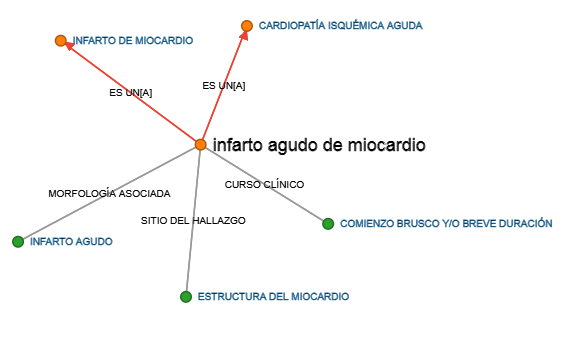
\includegraphics[width=0.9\textwidth]{infarto_agudo_miocardio}
\end{figure}


\subsubsection{Modelo de Conceptos de Snomed CT}
La organización jerárquica de Snomed CT permite pasar de conceptos más genéricos a más específicos \cite{Bhattacharyya2016}. El modelo define la forma en que los conceptos están dispuestos dentro de los subtipos de jerarquía y los tipos de relaciones de atributos que se permiten entre conceptos \cite{Bhattacharyya2016,ihtsdo2016SG}. Como consecuencia, cada concepto debe pertenecer a una sola jerarquía.
% * <mariad.avila@hospitalitaliano.org.ar> 2017-07-02T20:04:44.802Z:
% 
% > grafo dirigido acíclico
% Definir grafo dirigido acíclico en grafos
% 
% ^.
 
Hay 19 jerarquías, no todas son usadas para representar conceptos clínicos. Las siguientes 8 jerarquías tienen reglas para definir atributos y crear conceptos clínicos según \acrshort{IHTSDO} \cite{ihtsdo2016EG}.

\begin{itemize}
\item \textbf{Hallazgo clínico}, representa los resultados de una observación clínica, evaluación o juicio e incluye estados clínicos normales y anormales. La jerarquía de hallazgo clínico incluye conceptos para representar diagnósticos.
\item Los \textbf{procedimientos} representan actividades realizadas en la prestación de servicios de salud. Incluyen no sólo los procedimientos invasivos sino también la administración de medicamentos, toma  de imágenes, educación, terapias y procedimientos administrativos.
\item Los \textbf{especímenes} representan entidades que se obtienen, usualmente de pacientes, para el análisis.
\item \textbf{Estructuras corporales}, representan estructuras anatómicas normales y anormales.
\item \textbf{Productos biológicos/farmacéuticos}, representan productos farmacéuticos (no dispositivos)
\item Las \textbf{situaciones de contexto explícito} representan conceptos en los que el contexto clínico se especifica como parte de una definición del mismo concepto. Esto incluye la presencia o ausencia de una condición, ya sea que el hallazgo clínico es actual, hace parte del pasado o está relacionado a alguien diferente al paciente. Ejemplos de estas situaciones de contexto explicito son: sospecha de cáncer de mama (SCTID: 134405005), antecedente de neoplasia maligna de mama (SCTID: 415076002) y antecedente familiar de neoplasia maligna de mama (SCTID: 429740004), respectivamente.
\item Los \textbf{eventos} representan las ocurrencias que excluyen a los procedimientos y las intervenciones.
\item Por último, los \textbf{objetos físicos }representan a los objetos naturales o hechos por el hombre.
\end{itemize}
 
La tabla \ref{jerarquiasLista} contiene las jerarquías usadas en la lista de problemas y la frecuencia de conceptos de Snomed CT. Se puede observar que las jerarquías más usadas son hallazgo clínico, situación con contexto explícito y procedimientos.

% Please add the following required packages to your document preamble:
% \usepackage{booktabs}
\begin{table}[htb]
\centering
\caption{Jerarquías de la lista de problemas y frecuencias de uso}
\label{jerarquiasLista}
\resizebox{\columnwidth}{!}{%
\begin{tabular}{@{}lrr@{}}
\toprule
Jerarquía & Conceptos diferentes & Cantidad de problemas  \\ \midrule
Hallazgo clínico  & \num{82732} & \num{13594650} \\
Situaciones de contexto explícito  & \num{5086} & \num{1222531} \\
Procedimiento & \num{14991} & \num{1138167} \\
Otras Jerarquías  & \num{1122} & \num{144553} \\
Evento & \num{298} & \num{40084}\\
Estructura Corporal  & \num{186} & \num{11274}\\
Producto biológico/farmacéutico & \num{35} & \num{2040} \\
Objeto Físico  & \num{75} & \num{1285} \\ \bottomrule
\end{tabular}
}
\end{table}

\subsubsection{\textit{Reference set}}
\label{par:refset}
Para facilitar el uso de Snomed CT se construyen \textit{\acrfull{refset}}, que son conjuntos de conceptos en determinados dominios como especialidades, cohortes, tipos de enfermedades, etc. Estos dominios se llaman subconjuntos simples.

Uno de los aspectos claves en el uso significativo de la terminología es la creación de \textit{\acrshort{refset}} que puedan ser utilizados como vocabularios controlados para contextos específicos. Estos \textit{\acrshort{refset}} facilitan el uso de Snomed CT como terminología de codificación primaria para la lista de problemas u otros niveles de documentación clínica, y maximizan potencialmente la interoperabilidad de datos a través de las instituciones\cite{Dolin2004KaiserTerminology.}.Snomed CT no define metodologías para construir \textit{\acrshort{refset}} con conceptos que se agrupen por un contexto. La metodología propuesta en esta tesis agrupa los conceptos usados en el registro histórico de la lista de problemas según el contexto dado por el área jerárquica, el grupo etario y el nivel de asistencia con el que fue registrado. 

Existen \textit{\acrshort{refset}} públicos con características similares a los que se analizan en esta tesis. Estos \textit{\acrshort{refset}} fueron compilados por la organización Kaiser Permanente\label{par:kaiser-permanente} con el consenso de todos sus centros médicos\footnote{Kaiser Permanente es la organización de mantenimiento de salud, sin fines de lucro, más grande de los Estados Unidos (integra 28 centros médicos y tiene presencia en 8 estados). Es un sistema integrado de prestación de servicios de salud, que organiza y proporciona o coordina la atención de los miembros de la organización. Kaiser Permanente construyó una solución de terminología médica para toda la organización llamada \textit{\acrfull{CMT}}, que son subconjuntos de terminología adaptada a pacientes y médicos, vinculada a los estándares de interoperabilidad de Estados Unidos e internacionales. Desde el año 2010 donan estos subconjuntos a la \textit{\acrfull{UMLS}}
}. Estos  \textit{\acrshort{refset}} son útiles para hacer comparaciones con los resultantes en los experimentos de este trabajo: \textit{Cardiology; Common Lab Procedures; Emergency Department; Endocrine,  Nephrology, and Urology; ENT, Gastroenterology, and Infectious Diseases; Hematology and Oncology; History and Family History; Injury; Mental Health; Miscellaneous Problem List ; Musculoskeletal; Neurology; Obstetrics and Gynecology; Ophthalmology; Orthopedics; Pediatrics; Primary Care; Radiology; Skin/Dermatology and Respiratory; Specimen Source and Specimen Type; Urology \& Nephrology; Vaccinations; Vascular Procedures List}.


\subsection{Lista de problemas en la \acrshort{HCE} del \acrshort{HIBA} }
\label{par:listaproblemas-HCE}
Cualquier usuario con acceso a la \acrshort{HCE} puede registrar un problema, este usuario puede pertenece a una área administrativa o asistencial del \acrshort{HIBA}. Por consiguiente, las áreas jerárquicas que tiene el \acrshort{HIBA} responden a necesidades operativas de la \acrshort{HCE}, y tienen diferentes niveles de agregación, por ejemplo: Sección de neurocirugía vascular hace parte de una área más general llamada Servicio de neurocirugía. También existen áreas jerárquicas con muy pocos registros o que son \textit{ad hoc} por ejemplo: Instituto universitario H.I., Programa de prevención del cáncer de colon hereditario, Laser en rinosinusología.

Además cada registro de la lista de problemas tiene asociado el nivel de asistencia que indica el ámbito en el que fue cargado el problema. Los niveles de asistencia son las diferentes modalidades de contacto que tiene el paciente con el hospital, asegurando una óptima atención en cada situación específica. En la \acrshort{HCE} el nivel de asistencia puede ser cualquiera de los siguientes valores:

\begin{itemize}
\item Ambulatorio: Se tiene definido cuándo empieza y cuándo termina esa atención. El paciente solicita previamente un turno ambulatorio.
\item Episodio ambulatorio: Se sabe cuándo empieza pero no cuándo termina; entonces la modalidad de registro cambia. En el ambulatorio generalmente hay alguien que longitudinalmente ve al paciente en distintos momentos.
\item Triage: Se genera cuando un paciente tiene un contacto con el hospital sin un turno previo, consiste en una revisión médica rápida que permite definir la prioridad de atención.
\item Guardia: Los pacientes críticos con inminencia de muerte o que ingresan con una patología aguda, de gravedad moderada o severa, pero sin muerte inminente por la misma. En este nivel de asistencia se espera que el alta del nivel se dé entre las 24 y 36 horas de su ingreso, pudiendo trasladarse a otro nivel asistencial del hospital, o a otro hospital, o más rara vez a su domicilio.
\item Internación: Tiene un periodo limitado del cuidado, el paciente es tratado por un episodio grave de una enfermedad, cuyas condiciones puedan resultar en un trauma o su muerte. Los tipos de internación son general, domiciliaria y geriátrica.
\end{itemize}


\subsection{Redes}
\subsubsection{Definición}
Las redes están presentes en casi cada aspecto de nuestra vida. La tecnología nos ubica en un mundo lleno de redes, las relaciones físicas o lógicas que establecemos con nuestro entorno constituyen una red en sí misma. Al final de la década del noventa, el avance y popularidad de los computadores cambió la manera como se entendían las redes. La capacidad de los computadores hizo posible acumular grandes bases de datos con estructuras de redes y analizarlas rápida y eficientemente. Esto permitió por primera vez, la comparación de datos de redes reales con los modelos existentes, en particular el modelo ER. Otra influencia importante de la revolución de la computación fue la creación y rápido desarrollo de dos redes enormes: la internet y la World Wide Web (WWW). 

En consecuencia, el concepto abstracto de una red cubre una amplia variedad de estructuras en las cuales las entidades de los sistemas complejos son representados por vértices o nodos y las relaciones o interacciones entre esas entidades son representadas con aristas o enlaces de la red \cite{Estrada2015ATheory}.A continuación presento algunos ejemplos de redes usadas en las áreas de biología y medicina, aunque en la literatura siguen surgiendo nuevos.

\subsubsection{Tipos de redes}
% * <mariad.avila@hospitalitaliano.org.ar> 2017-07-01T16:52:38.003Z:
% 
% Actualizar a 2017
% 
% ^.
 
\paragraph{Redes sociales:} Contempla las redes con interacciones entre individuos. Estos pueden consistir en redes de amigos o conocidos, relaciones de trabajo o sexuales. Además de su importancia en los estudios sociales, entender la estructura de estas redes es también importante para los epidemiólogos, ya que es por medio de estas redes que las epidemias se propagan. \cite{Cohen2010}
 
\paragraph{Redes biológicas:}Este tipo abarca diferentes tipos de redes, las redes biológicas pueden ser lógicas, representando interacciones entre proteínas, entre genes, o entre proteínas y genes. Interacciones entre moléculas en las vías metabólicas de la célula pueden ser vistas como una red. Aunque las interacciones son físicas, los enlaces no son entidades físicas sino la posibilidad de una interacción entre dos moléculas. Otras redes lógicas son las ecológicas predador-presa (donde los vértices son las especies, y los enlaces dirigidos representan la depredación de una especie por la otra). Otro tipo de redes biológicas son las redes biológicas físicas, como el sistema de nervios, las neuronas en el cerebro y la red de venas en un organismo. \cite{Cohen2010}
 
\paragraph{Redes de salud:} A continuación enumero algunos trabajos con redes en el área de la salud.
\begin{itemize}
\item La red de enfermedades humanas \cite{Goh2007TheNetwork.} es una red de trastornos y enfermedades genéticas vinculadas por genes en común. Esta red permite explorar el fenotipo y las enfermedades genéticas asociadas, indicando así el origen genético que tienen en común muchas enfermedades. El proyecto nació en el 2007, y para el 2014 se agregó la red de síntomas a partir de metadata de los encabezados de temas médicos (MeSH\footnote{MeSH por Medical Subject Headings, es el vocabulario controlado Biblioteca Nacional de Medicina. Este vocabulario se usa para indexar artículos para la base de datos MEDLINE y PubMED. Cada cita de los artículos se asocia con un conjunto de palabras claves MeSH que describen el contenido de la cita.}) de PubMED. A partir de estas redes se han hecho múltiples trabajos que explican la interacción entre enfermedades, interacciones entre proteínas, interacciones de enfermedades con drogas y comorbolidades.
\item La red de medicina \cite{Haaren2013,Barabasi2011NetworkDisease}, fue creada  bajo la premisa de que una enfermedad es rara vez consecuencia de una anormalidad en una sola parte del sistema corporal del paciente. Esto implica que las redes deben ilustrar el impacto y la complejidad de la asociación de las enfermedades, además que estas enfermedades pueden ser agrupadas y segmentadas.
\end{itemize}

\subsection{Grafos}
Los grafos se usan para describir de forma matemática relaciones entre redes. Los grafos representan las propiedades topológicas esenciales de una red mediante el tratamiento de ésta como una colección de nodos y enlaces. Este enfoque permite usar herramientas y métodos matemáticos para realizar cálculos en redes complejas.

En su definición es un conjunto de pares ordenados $G=(V,E)$ tal que $E\subseteq [V]^{2}$, así cada elemento de $E$ está asociado a un par de elementos (el mismo o distinto) de $V$. Los elementos de $V$ se llaman vértices (o nodos) de G, y los elementos de $E$ se llaman aristas de G.\cite{Diestel2005GraphTheory,Balakrishnan2000ATheory} 

\subsubsection{Conceptos relacionados a los grafos}

Se comentan y describen algunos términos acerca de grafos, siguiendo las definiciones de Diestel \cite{Diestel2005GraphTheory}:

\paragraph{Orden}
El número de vértices de un grafo, o su cardinalidad, es su \textbf{orden}, y se escribe como $|G|$; el número de aristas se denota con $||G||$. Los grafos son finitos o infinitos de acuerdo a su orden. Un \textbf{grafo vacio} de orden 0 o 1 se llama \textbf{trivial}. Los grafos que se estudian en esta tesis son todos finitos y no triviales.

\paragraph{Adyacencia}
Dos vértices $u$ y $v$ de $G$ son \textbf{adyacentes} o \textbf{vecinos} si $u$ y $v$ son los vértices finales de una arista de $G$. Las dos aristas $e\neq f$ son \textbf{adyacentes} si tienen un vértice en común. 

\paragraph{Grafo completo y triángulo}
Si todos los vértices de $G$ son adyacentes entre si, entonces se dice que $G$ es \textbf{completo}. Un \textbf{grafo completo} de $n$ vértices se denota como $K^{n}$. $K^{3}$ se llama \textbf{triángulo}.

\paragraph{Vértices y aristas independientes}
Los vértices o aristas que no son adyacentes a ningún otro se llaman \textbf{independientes}

\paragraph{Grado}
El \textbf{grado} de un vértice $v$ $|E(v)|$ es el número  de aristas de $v$, es decir el número de vértices adyacentes a $v$. Un vértice de grado 0 es \textbf{independiente}.

\paragraph{Subgrafo}
Sea $G\cup  G':=(V\cup  V', E\cup  E')$ y $G\cap  G':=(V\cap  V', E\cap  E')$. Si $G\cap G' = 0$  entonces $G$ y $G'$ son \textbf{disjuntos}. Si  $V'\subseteq V$ y $E'\subseteq E$, entonces $G'$ es un \textbf{subgrafo} de $G$ (y $G$ es un \textbf{supergrafo} de $G'$), la notación es $G'\subseteq G$. Formalmente se dice que $G$ contiene a $G'$.

\paragraph{Caminos y ciclos}
Un \textbf{camino} es un grafo no trivial $P=(V,E)$ de la forma 
\begin{equation}
V={x_{0},x_{1},...,x_{k}}, E={x_{0}x_{1},x_{1}x_{2},...,x_{k-1}x_{k}}
\end{equation}

donde las $x_{i}$ son todas distintas. Los vértices $x_{0}$ y $x_{k}$ están enlazados por $P$ y se llaman vértices \textbf{terminales}. Los vértices $x_{1},...,x_{k-1}$ son los vértices \textbf{internos} de $P$. El número de aristas de un camino es su \textbf{longitud}.

Una notación usual para representar un camino es la secuencia de sus vértices, de tal forma que $P=x_{0}x_{1}...x_{k}$ se denota como camino $P$ de $x_{0}$ a $x_{k}$ (también entre $x_{0}$ y $x_{k}$).

Si $P=x_{0}...x_{k-1}$ es un camino y $k\geq 3$, entonces el grafo $C:=P+x_{k-1}x_{0}$ se llama un \textbf{ciclo}. Se denomina ciclo por su (cíclica) secuencia de vértices, el ciclo anterior se escribe como $x_{0}...x_{k-1}x_{0}$.

\paragraph{Grafos dirigidos}
Un \textbf{grafo dirigido} es un par $(V,E)$ de conjuntos disjuntos de vértices y aristas que juntos forman dos mapas (1) inicial: $E\rightarrow V$ y (2) terminal: $E\rightarrow V$, asignándole a cada arista $e$ un \textbf{vértice inicial} $inicial(e)$ y un \textbf{vértice termina}l $terminal(e)$. Se dice que la arista $e$ se dirige desde $inicial(e)$ a $terminal(e)$.

\paragraph{Grafo de Snomed CT}
Al diseccionar la estructura de Snomed CT, cada concepto se representa con un vértice y cada relación entre los conceptos se representa por una arista. No hay relaciones circulares y todas son unidireccionales sin excepciones, pero un vértice $inicial(e)$ puede tener más de una relación de salida o vértices $terminal(e)$, de esta manera se construye un grafo acíclico dirigido. \cite{Bhattacharyya2016}

\subsubsection{Patrones de grafos en redes}
La mayoría de las redes de gran escala comparten patrones que no se notan en redes pequeñas. Entre todos los patrones, la mayoría de las características más conocidas son: \textbf{distribución libre de escala, efecto de mundo pequeño y fuertes estructuras de comunidad}.\cite{Tang2010}

\paragraph{Distribución libre de escala} \cite{Tang2010}.
\label{par:definicion-libre-escala}
Los grados de los vértices en las redes de gran escala a menudo siguen una distribución de ley de potencia, también conocidas como distribución Zipfian o distribución Pareto. 

En su definición, una variable aleatoria $X$ sigue una distribución de ley de potencia si
\begin{equation}
p(x)=Cx^{-\alpha}, x\geq  x_{min}; \alpha \geq 1
\end{equation}

De tal manera que $\alpha \geq 1$ asegura que exista una constante de normalización $C$. Una distribución que sigue la ley de potencia se llama también  distribución sin escalas, ya que la forma de la distribución permanece sin cambios, excepto para una constante multiplicativa general, cuando la escala de unidades se incrementa por un factor. Esto es
\begin{equation}
p(ax)=bp(x)
\end{equation}
 
Donde $a$ y $b$ son constantes. En otras palabras, no existe una escala característica con la variable aleatoria. La forma funcional es la misma para todas las escalas. La red con una distribución libre de escalas para los grados nodales también se denomina \textbf{red libre de escala}.
 
Mientras que para las distribuciones normales, es extremadamente raro que un evento ocurra con una desviación muy lejana de la media, en las distribuciones de ley de potencias la cola es mucho más larga. De tal manera, es común que algunos vértices de la red tengan alto grado mientras que la mayoría tengan pocas conexiones. La razón es que la cola de una distribución de ley de potencias decae polinomialmente. Esto es asintotáticamente más lento que en la distribución normal que lo hace exponencialmente, resultando en un fenómeno de cola pesada. La curva de la distribución de ley de potencias se convierte en una recta si graficamos la distribución en una escala log-log, ya que
\begin{equation}
\log p(x) =-\alpha \log x + \log C
\end{equation}
Esta asociación se puede usar para verificar graficamente si la distribución sigue la ley de potencias. Una verificación más robusta es aproximar la función de \acrfull{cdf} descripta con la siguiente ecuación:
\begin{equation}
F(X\geq x) \propto  x^{-\alpha+1 }
\end{equation}

\paragraph{Métricas de comunidades}
\label{par:efecto-comunidades}
Informalmente, una comunidad es un conjunto de vértices donde cada vértice es más cercano a otros vértices en su comunidad que a los vértices que están fuera de ella. Esta característica ha sido encontrado especialmente en las redes sociales \cite{Tang2010}. La figura \ref{fig:ejemploCluster} ilustra las comunidades que se forman a partir de las relaciones de los vértices, cada color representa una comunidad.

\begin{figure}
\caption{Ejemplo de comunidades}
\label{fig:ejemploCluster}
\centering
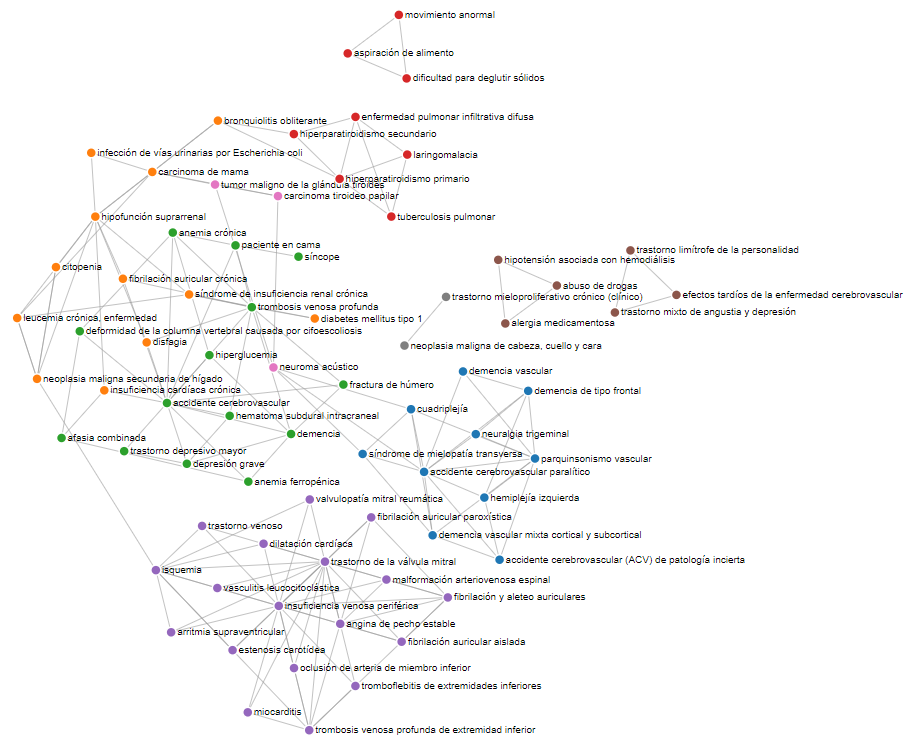
\includegraphics[width=\textwidth]{ejemplo_cluster.png}
\end{figure}

La fuerza de las comunidades se miden con diferentes métricas, en esta tesis se analiza el coeficiente de agrupamiento global o \textbf{transitividad}, el coeficiente de agrupamiento promedio y la longitud media del camino mínimo entre vértices. 

\subparagraph{Coeficiente de agrupamiento - Transitividad}
La transitividad \cite{Wasserman1994} $C^{\Delta}$, se calcula como una medida de la proporción de triángulos cerrados en un grafo:
\begin{equation}
\label{equ:coeficiente_transitividad}
C^{\Delta} =3\cdot\frac{\text{número de triángulos}}{\text{número de tripletas conectadas}}
\end{equation}
Esta métrica muestra de manera global cuán agrupado es el grafo, ya que representa la probabilidad de que dos vértices estén conectados si comparten un vecino en común. En el contexto de la lista de problemas, si los problemas $P1$, $P2$ co-ocurren en pacientes que también tengan $P3$, esta métrica representa la probabilidad de que $P1$ y $P2$ ocurran juntas.

\subparagraph{Coeficiente de agrupamiento - Promedio}\cite{Saramaki2006,Kaiser2008}
El promedio del coeficiente de agrupamiento del grafo G, necesita del cálculo local de los coeficientes de agrupamiento de cada vértice i. En el caso de los grafos dirigidos,

\begin{equation}
c_{i} = \frac{\Gamma_{v_{i}}}{|E(v_{i})|(|E(v_{i})|-1)},
\end{equation}

donde $|E(v_{i})|$ es el grado del vértice $v_{i}$ y $\Gamma_{v_{i}}$ es el número de aristas entre los vecinos de $v_{i}$.

Finalmente, el coeficiente de agrupamiento se calcula con la siguiente ecuación.
\begin{equation}
\label{equ:coeficiente_promedio}
C = \frac{1}{n}\sum_{v \in G} c_v,
\end{equation}

Donde $n$ es el número de vértices evaluados. 

El coeficiente de agrupamiento promedio produce una alta varianza para los vértices con menos grados. Por ejemplo, para vértices con grado 2, $C_{i}$ es 0 o 1.\cite{Tang2010} %%Se usa comúnmente para estudios numéricos mientras que la \textbf{transitividad} se utiliza más para el estudio analítico.%%

La figura \ref{fig:ejemplocoeficienteagrupamiento} muestra en los ejemplos a), b) y c) el cálculo del coeficiente de agrupamiento del vértice i en azul. En el ejemplo d) está el cálculo de cada nodo. Siguiendo las ecuaciones \ref{equ:coeficiente_promedio} y \ref{equ:coeficiente_transitividad}, el coeficiente de agrupamiento promedio es de \num{0.310} y la transitividad es de \num{0.375}, respectivamente.

\begin{figure}
\caption{Ejemplos de coeficientes de agrupamiento}
\label{fig:ejemplocoeficienteagrupamiento}
\centering
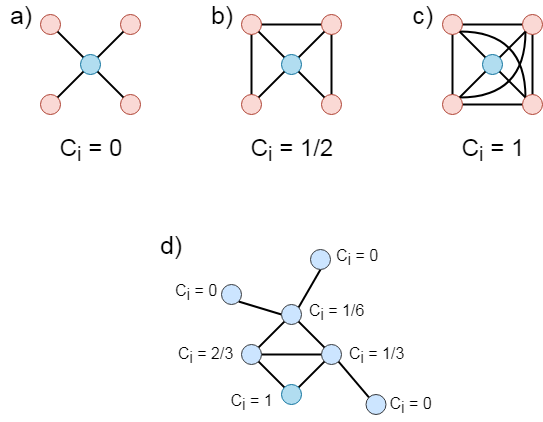
\includegraphics[width=0.8\textwidth]{Images/coeficiente_de_agrupamiento.png}
\end{figure}

\subparagraph{Longitud media del camino mínimo entre vértices}
Cálculo de la media de la distancia entre los vértices en un grafo. Comunidades con longitudes medias más pequeñas indican estructuras de comunidades más fuertes.

\subparagraph{Distancia semántica}
La distancia semántica se usa para calcular similaridad entre conceptos. En diferentes trabajos en el dominio médico \cite{Wang2010,Gan2013,Pedersen2007,Zare2015ASNOMED-CT} se presentan diferentes maneras más sofisticadas de calcular la similaridad que la longitud media del camino mínimo. Sin embargo, estos enfoques son también alguna variante de la longitud media del camino mínimo.
El modelo de datos define la arista "$|\text{ES UN}|$" para establecer relaciones entre conceptos ancestros y descendientes, de tal manera que todos los conceptos son un subtipo de otro más general, y un concepto puede tener uno o más descendientes con varios niveles de especificación.


\subsection{\textit{Graphmining}}
La minería de datos se ha convertido en sinónimo de encontrar patrones frecuentes en datos transaccionales, el término más general descubrimiento de conocimiento abarca esta y otras tareas. Descubrimiento o aprendizaje no supervisado en \textit{graphmining} implica no sólo la tarea de encontrar patrones en un conjunto de transacciones, sino también encontrar la posible superposición de patrones en un gran grafo. Descubrimiento también implica la tarea de \textbf{\textit{clustering}}, la cual intenta describir todos los datos por medio de la identificación de clases de grafos que comparten patrones comunes de atributos y relaciones entre sí. \textit{Clustering} también puede extraer relaciones entre \textit{clusters}, resultando en una organización jerárquica o taxonómica.\cite{Cook2006}
 
En contraste, el aprendizaje supervisado es la tarea de extraer patrones que distinguen un conjunto de otros. Estos conjuntos se llaman los ejemplos positivos y los negativos. Este conjunto de ejemplos pueden contener muchas transacciones de grafos o un sólo gran grafo. El objetivo es encontrar un patrón de relación entre nodos que aparezca a menudo en los ejemplos positivos pero no en los ejemplos negativos. Tal patrón se usa para predecir la clase (positiva o negativa) de nuevos ejemplos. \cite{Cook2006}
 
La última tarea en graph mining es la visualización del conocimiento descubierto. La visualización de grafos es la representación de los vértices, aristas y etiquetas de un grafo de tal manera que los humanos entiendan los conceptos representados por el grafo.\cite{Cook2006}

\subsubsection{Análisis de redes}
El análisis de redes involucra una variedad de tareas \cite{Tang2010}, a continuación listo las que aplicaré en este trabajo:

\begin{enumerate}
  \item Análisis de centralidad, ayuda a identificar los vértices (o problemas en el contexto de esta tesis) “más importantes” en la red. Esta importancia puede definirse de distinta manera y cada una ayuda a entender diferentes aspecto de la influencia y el poder del vértice en la red:
  
\begin{itemize}
\item \textbf{Centralidad de grado.}
Cuenta el número de conexiones que tiene un vértice. Los problemas con los grados más altos serán los que más ocurren en los pacientes.
\item \textbf{Intermediación (\textit{betweenness}).} Mide el número de veces que un vértice en particular es miembro de los caminos más cortos entre otros dos vértices.
Usualmente, la medida de intermediación está normalizada en el rango de [0, 1], dónde 0 es un vértice desconectado y 1 un vértice por donde pasan todas las conexiones.\cite{Cook2006,Brath2015GraphData}
\item \textbf{Cercanía (\textit{Closeness}).} La cercanía de un vértice mide la distancia promedio a todos los otros vértices. Si pocos vértices son alcanzables o si la distancia entre los vértices aumenta, entonces la medida de cercanía es pequeña. \cite{Cook2006,Brath2015GraphData}.
\item \textbf{Centralidad de autovector (\textit{Eigenvector}).} Dado un vértice, se suma recursivamente todas las distancias a todos los otros vértices. Entre más centrales sean los otros vértices, el vértice que se está midiendo tendrá mayor centralidad\cite{Brath2015GraphData}.
\end{itemize}
\item Clasificación de redes y detección de \textit{outliers}. Algunos problemas están etiquetados con información contextual: servicio de salud, ámbito y grupo etario. Por ejemplo, en una red con algunos problemas pocos comunes identificados como del Servicio Cardiológico, ¿es posible inferir otros problemas poco comunes asociados por su co-ocurrencia en los pacientes?
  \item \textit{Clustering}. Según Blonde et al.\cite{Blondel2008FastNetworks}, el problema de \textit{clustering} requiere la partición de una red en grupos de vértices densamente conectados, donde los vértices que pertenecen a diferentes grupos se conectan escasamente. Las formulaciones exactas de este problema de optimización son computacionalmente intratables. En los últimos años se han propuesto muchos algoritmos para encontrar particiones razonablemente buenas de una manera razonablemente rápida, debido al incremento de la disponibilidad de conjuntos de datos con grandes redes y el impacto de las redes en la vida. Se pueden distinguir los siguientes tipos de algoritmos \label{par:algoritmos-nosupervisados}:
\begin{itemize}
\item \textbf{Divisivos:} Se comienza con todo el grafo y se van eliminando iterativamente las aristas, dividiendo así progresivamente el grafo en subgrafos desconectados más y más pequeños. Estos subgrafos se identifican como comunidades. El punto crucial en un algoritmo divisivo es la selección de las aristas que se van a eliminar, las cuales deben ser las que conectan comunidades y no las aristas que están dentro de las comunidades. \cite{Radicchi2004DefiningNetworks,Girvan2002CommunityNetworks.,Newman2004FastNetworks}
\item \textbf{Aglomerativos:} Para cada uno de los vértices del grafo se calcula un peso, el cual mide qué tan conectados están los vértices. A partir del conjunto de todos los vértices sin aristas, se ordenan decrecientemente los vértices según su pesos, y se agregan iterativamente las aristas entre pares similares de vértices. De esta manera, los vértices se agrupan en comunidades cada vez más grandes, y el árbol se construye hasta la raíz. Este árbol representa a todo el grafo. \cite{Radicchi2004DefiningNetworks,Pons2005ComputingWalks}
\item \textbf{Optimización:} Estos algoritmos buscan encontrar resultados usando heurísticas o maximizando una función objetivo con un enfoque voraz (\textit{greedy}) para mejorar la complejidad computacional de los algoritmos clásicos. Estos métodos consisten en unir recursivamente las comunidades buscando optimizar la función objetivo.\cite{Clauset2004FindingNetworks,Blondel2008FastNetworks}
\end{itemize}
  
\end{enumerate}

\subsubsection{Evaluación de estructuras}
La detección de comunidades es el tópico que se desarrolla en mayor profundidad en esta tesis. Se usan los tres enfoques principales y se comparan los resultados. En parte, la razón por la cual hay tantas definiciones y métodos, es que no está clara cómo debe ser la estructura de una comunidad en una red real. De tal manera que diferentes métodos se desarrollaron según las necesidades de sus autores \cite{Tang2010}.

Para poder comparar los diferentes resultados obtenidos con los algoritmos, utilizaré las siguientes estrategias:

\begin{itemize}
\item Cálculo de modularidad
\item Comparación de las comunidades con un \textit{gold-standard }
\end{itemize}

\paragraph{Cálculo de modularidad.}
 
Según Newman \cite{Newman2006FindingMatrices.}, una buena división de una red en comunidades no es solamente aquella en la que el número de aristas  entre los grupos es pequeño, sino en la que el número de aristas entre los grupos es menor al esperado. Sólo si el número de aristas entre los grupos es significativamente más bajo al esperado se puede decir con justificación que se ha encontrado una estructura de comunidad significativa. Equivalentemente, se puede examinar el número de aristas dentro de las comunidades y buscar divisiones de las redes en las cuales este número es más alto del esperado, los dos enfoques son equivalentes. Estas consideraciones constituyen una medida basada en un punto de corte para modificar una función de beneficio $Q$ definida como
\begin{equation}
Q =  (\text{Número de aristas en la comunidad}) -  (\text{Número de aristas esperadas})
\end{equation} 

Esta función de beneficio se llama \textbf{modularidad}. La modularidad de una partición es un valor escalar entre -1 y 1. La modularidad mide la densidad de los enlaces en las comunidades comparándola con los enlaces entre las comunidades\cite{Blondel2008FastNetworks}. Valores cercanos a 1 indican estructuras de comunidades más fuertes, y valores cercanos a -1 indican que los nodos están agrupados en comunidades a las que no pertenecen\cite{Tang2010}.

\paragraph{Comparación de las comunidades con un \textit{gold-standard}.}
\label{par:cubrimiento}

El término \textit{gold-standard} \cite{Versi1992GoldTerm.} se utiliza en los trabajos científicos para referirse a valores de referencia que están disponible en condiciones razonables. No es la prueba perfecta, sino la mejor disponible. El \textit{gold-standard} es importante ante la imposibilidad de realizar mediciones directas para determinar si los conceptos que están dentro de una comunidad realmente pertenecen o no a ella. Los \textit{gold-standard} con el que se realizan las mediciones son los públicos y disponibles por la organización Kaiser Permanente (Ver sección \ref{par:kaiser-permanente}).

La medición que se realizó se llama cubrimiento, la cual se define como la proporción de los conceptos que se comparten entre los dos conjuntos de datos, al tamaño del \textit{\acrshort{refset}} (Ver sección \ref{par:refset}) de referencia $T$, como se define en la ecuación \ref{eq:cubrimiento}

\begin{equation}\label{eq:cubrimiento}
\textup{cubrimiento} = \frac{\textup{conceptos mapeados en T}}{\textup{Tamaño de T}}
\end{equation}

\begin{itemize}
\item \textit{Conceptos mapeados en T}, es el número total de conceptos de Snomed CT que comparten el \textit{refset} que se compara y el \textit{refset} $T$, y
\item el \textit{tamaño de T} es el número total de conceptos que tiene el \textit{refset} $T$.
\end{itemize}

\section{Objetivos}
Con el presente trabajo se contribuye a la organización de los datos y el uso significativo de Snomed CT para la recuperación de información en la lista de problemas del Hospital Italiano de Buenos Aires. Esta contribución es la construcción de una taxonomía de problemas, cuyas relaciones son ponderadas por su co-ocurrencia en las listas de problemas de los pacientes y sus relaciones jerárquicas con Snomed CT.

El producto final de este trabajo es el modelo que representa grupos o clasificaciones y las relaciones significativas de los problemas que co-ocurren en los pacientes. Los experimentos para llegar a este modelo tendrán en cuenta la lista de problemas y se añadirá  información de contexto: ámbito o nivel de asistencia, área jerárquica y grupo etario. La comparación entre los modelos y la evaluación de su capacidad predictiva se hará con las medidas de precisión y exactitud. 

\section{Organización del trabajo}
% * <mariad.avila@hospitalitaliano.org.ar> 2017-07-01T16:27:48.600Z:
% 
% Cómo va a estar organizada la tesis
% 
% ^.
En el capítulo 2 se explica la metodología, se describen los algoritmos y los criterios de evaluación.

En el capítulo 3 hago una descripción de los datos y las decisiones en la limpieza de datos. Luego, se aplican las técnicas de \textit{graphmining}.
 
Por último en el capítulo 4, hablo sobre las conclusiones y futuros pasos.


\chapter{Capítulo: Metodología}
%%%% Metodologia
\section{Introducción}
Tomando como base la metodología \textit{\acrfull{CRISP-DM}} divido el trabajo en fases, describo los procesos que se realizan en cada una de ellas y los entregables que servirán de insumo para la siguiente fase.

En las primeras fases estudio el problema y los datos. La siguiente fase, que es la preparación de los datos genero el conjunto de entrenamiento con los registros previos al año 2017, y el conjunto de validación con los registros del año 2017. En las fases de diseño y evaluación, ejecuto los algoritmos de aprendizaje no supervisado con el fin de encontrar grupos significativos con alto valor de precisión y exactitud. En la fase final se organizan los datos y  redacto el documento final.

\section{Algoritmos de aprendizaje no supervisado}
\label{par:aprendizaje_nosupervisado}
El paquete igraph\cite{igraph} de Python ofrece una variedad de algoritmos para realizar aprendizaje no supervisado. Sin embargo, por el tamaño del grafo algunos algoritmos son imposibles de usar en la práctica. Por ejemplo, el método \textit{leading edge betweenness} para detectar comunidades tiene una complejidad $O(|E||V|^2)$ en el peor caso (donde $|V|$ número de vértices y $|E|$ número de aristas). Para procesar el grafo de la red semántica de problemas se necesitaría 181.93 años. Los detalles de otros algoritmos para la generación de comunidades del paquete igraph se encuentran en la tabla \ref{algoritmos_igraph}.

\begin{table}[tbp]
\centering
\caption{Algoritmos de aprendizaje no supervisado del paquete igraph}
\label{algoritmos_igraph}
\begin{threeparttable}
\begin{tabularx}{\textwidth}{@{}XXXX@{}}
\toprule
Algoritmo & Observaciones & Complejidad\tnote{1}  & Cálculo de tiempo de ejecución\tnote{2} \\ \midrule
\textit{spinglass} & Comunidades basadas en la física estadística & No especificado &  \\
\textit{leading} \newline  \textit{eigenvector} & Comunidades basadas en matrices de autovectores & $O(|E|+|V|^2*steps)$, donde “steps” es atributo del algoritmo & 6.86 segundos \\
\textit{walktrap} & Comunidades basados en caminos aleatorios & $O(|E||V|^2)$ en el peor caso, $O(|V|^2 log|V|)$ en promedio, & 181.93 años en el peor caso, 38 segundos en el caso promedio \\
\textit{edge} \newline \textit{betweenness} & Comunidades basados en la métrica de centralidad intermediación & $O(|E||V|^2)$ en el peor caso & 181.93 años en el peor caso \\
\textit{fast greedy} & Comunidades basadas en optimización de la modularidad & $O(|E||V|log|V|)$ en el peor caso, $O(|E|+|V|log^2|V|)$ en promedio & 22.84 minutos en el peor caso, 0.0011 segundos en promedio \\
\textit{multilevel} & Comunidades mediante la optimización de la modularidad multinivel & En promedio lineal en grafos dispersos & 0.00064 segundos en promedio \\
\textit{label} \newline  \textit{propagation} & Comunidades basadas en la propagación de etiquetas & $O(m+n)$ & Depende del tamaño de la matriz resultante. \\
\textit{infomap} & Estructuras de comunidades que minimizan el valor esperado & No especificado &  \\ \bottomrule
\end{tabularx}
\begin{tablenotes}
    \item[1] donde $|V|$ número de vértices, $|E|$ número de aristas.
    \item[2] Cálculos basados en números de instrucciones por segundos en un procesador AMD Athlon FX-60 (Dual Core) Reloj 2.6 GHZ = 22150 MIPS.
  \end{tablenotes}
\end{threeparttable}
\end{table}

Seleccioné los siguientes algoritmos para realizar todos los experimentos de aprendizaje no supervisados, teniendo en consideración la complejidad computacional y escogiendo un representante de cada uno de los tipo de algoritmos mencionados en el capítulo anterior (divisivos, aglomerativos y optimización) (Ver sección \ref{par:algoritmos-nosupervisados}).

\subsection{Algoritmo: \textit{leading eigenvector}}\cite{Newman2006FindingMatrices.} 
\begin{itemize}
\item Complejidad: $c|V|^2 + |E|$
\item Tipo de algoritmo: Optimización
\end{itemize} 
El algoritmo \textit{Leading Eigenvector} implementado por igraph usa un algoritmo recursivo para detectar estructura de comunidades. Este algoritmo divide la red maximizando la modularidad respecto a la red original. 
 
Los métodos basados en este enfoque han tenido excelentes resultados en test estandarizados. Desafortunadamente, la optimización exhaustiva de la \textbf{modularidad} requiere grandes esfuerzos computacionales, incluyendo algoritmos voraces (\textit{greedy}), enfriamiento simulado (\textit{simulated annealing}) y optimización extrema (\textit{EO}). El algoritmo desarrollado por Newman tiene un enfoque diferente. Se reescribe la función de \textbf{modularidad} en términos de la matriz, lo cual permite expresar la tarea de optimización como un problema espectral en el álgebra lineal. Este enfoque lidera una familia de algoritmos rápidos para detectar comunidades que producen resultados que compiten con los mejores métodos previos a él.
 
\subsection{Algoritmo: \textit{multilevel}}\cite{Blondel2008FastNetworks} 
\begin{itemize}
\item Complejidad: ``lineal'' cuando  $|V|$ es aproximadamente igual a $|E|$, el algoritmo sugiere que podría ser cuadrática con los grafos completamente conectados.
\item Tipo de algoritmo: Aglomerativo
\end{itemize}
El tamaño típico de las grandes redes se cuenta en millones cuando no miles de millones de vértices. Ejemplos de estas redes son las sociales, las telefónicas móviles o la web. En esta escala se demanda nuevos métodos para recuperar información a partir de su estructura. Un enfoque prometedor consiste en la descomposición de redes en subunidades o comunidades. La identificación de estas comunidades es de crucial importancia ya que pueden ayudar a descubrir módulos funcionales desconocidos a priori, tales como tópicos en redes de información o ciber comunidades en redes sociales. Además, las meta redes resultantes, cuyos vértices son comunidades, pueden ser usadas para visualizar la estructura de la red original.
 
El algoritmo \textbf{multilevel} encuentra particiones con alta \textbf{modularidad} en grandes redes en poco tiempo y despliega una completa estructura de comunidad jerárquica para una red, dando así acceso a diferentes resoluciones de una detección de comunidades. El algoritmo se divide en dos fases que se repiten iterativamente. Asume que se empieza con una red ponderada de $N$ vértices. Primero, se asigna una comunidad diferente a cada vértice de la red. De esta manera, en esta partición inicial hay tantas comunidades como vértices. Entonces, por cada vértice $i$ se evalúa si mejora la \textbf{modularidad} al cambiar la comunidad asociada al vértice $i$ por las comunidades en las que están cada uno de vértices adyacentes a él. El vértice $i$ es entonces puesto en la comunidad en la cual la modularidad es máxima y positiva. Si no se obtiene una ganancia positiva, entonces el vértice $i$ se mantiene en su comunidad original. Este proceso se aplica repetidamente y de manera secuencial para todos los vértices hasta que no se puede lograr ninguna mejora.
 
\subsection{Algoritmo: \textit{label propagation}}\cite{Raghavan2007NearNetworks.}
\begin{itemize}
\item Complejidad: $|V| + |E|$
\item Tipo de algoritmo: Divisivo
\end{itemize}
Cada vértice tiene una etiqueta inicial. En cada iteración del algoritmo se usa una función uniforme para determinar las aristas que son eliminadas, en el siguiente paso cada vértice adopta la etiqueta que es mayoritaria en los vértices adyacentes. A medida que las etiquetas se propagan a través de la red, grupos de nodos densamente conectados constituyen un consenso en sus etiquetas. 

Hay dos condición posibles de parada. En la primera puede ser que se llegue a la convergencia, es decir que la mayoría de los vecinos de cada vértice tengan la misma etiqueta que dicho vértice. La segunda es que se fija la cantidad máxima de iteraciones. 

Al final del algoritmo, los nodos con la misma etiqueta son conectados como comunidad. 

Las ventajas de este algoritmo sobre otros métodos es su simplicidad y su efectividad en el tiempo. El algoritmo usa la estructura de la red para guiar su progreso y no optimiza alguna métrica específica. Además, el número de comunidades y sus tamaños no se conocen a priori y se determinan cuando finaliza el algoritmo.
 
Aunque las redes con una sola comunidad satisfacen el criterio de parada, romper los enlaces aleatoriamente permite que se generen subgrafos disjuntos, evitando así que la misma etiqueta se propague por todo el grafo. En el caso de redes homogéneas que no tienen estructura de comunidades, el algoritmo identifica la red como una sola comunidad.


\section{Metodología CRISP-DM}
En el desarrollo de proyectos de minería de datos y descubrimiento de conocimiento, la metodología que más se usa es \textit{\acrshort{CRISP-DM}}. \acrshort{CRISP-DM} es una metodología independiente de dominio, por lo que puede utilizarse con cualquier herramienta de minería de datos y se puede aplicar para resolver cualquier problema de minería de datos.\cite{Marbn2009AModel}

Este trabajo se divide en seis fases (ver Figura \ref{fig:Metodologia}). Todas las fases usan transversalmente el mismo software: Oracle para el modelo de datos ER, Neo4J\footnote{Neo4j (\url{https://neo4j.com/}) es un proyecto de código abierto que permite implementar el modelo de bases de datos de grafos. Es la solución empresarial que más se usa, combina la fortaleza del almacenamiento nativo de grafos y una arquitectura escalable y optimizada para asegurar un buen rendimiento en las consultas basadas en relaciones} para el modelo de datos de grafos, Python y Java para la limpieza, selección de datos y ejecución de modelos, y las librerías de javascript D3.js y linkurious.js para la visualización de los datos. 
A continuación describo lo que contempla cada fases de esta tesis.

\begin{figure}[ht]
\caption{Metodología del trabajo de tesis}
\label{fig:Metodologia}
\centering
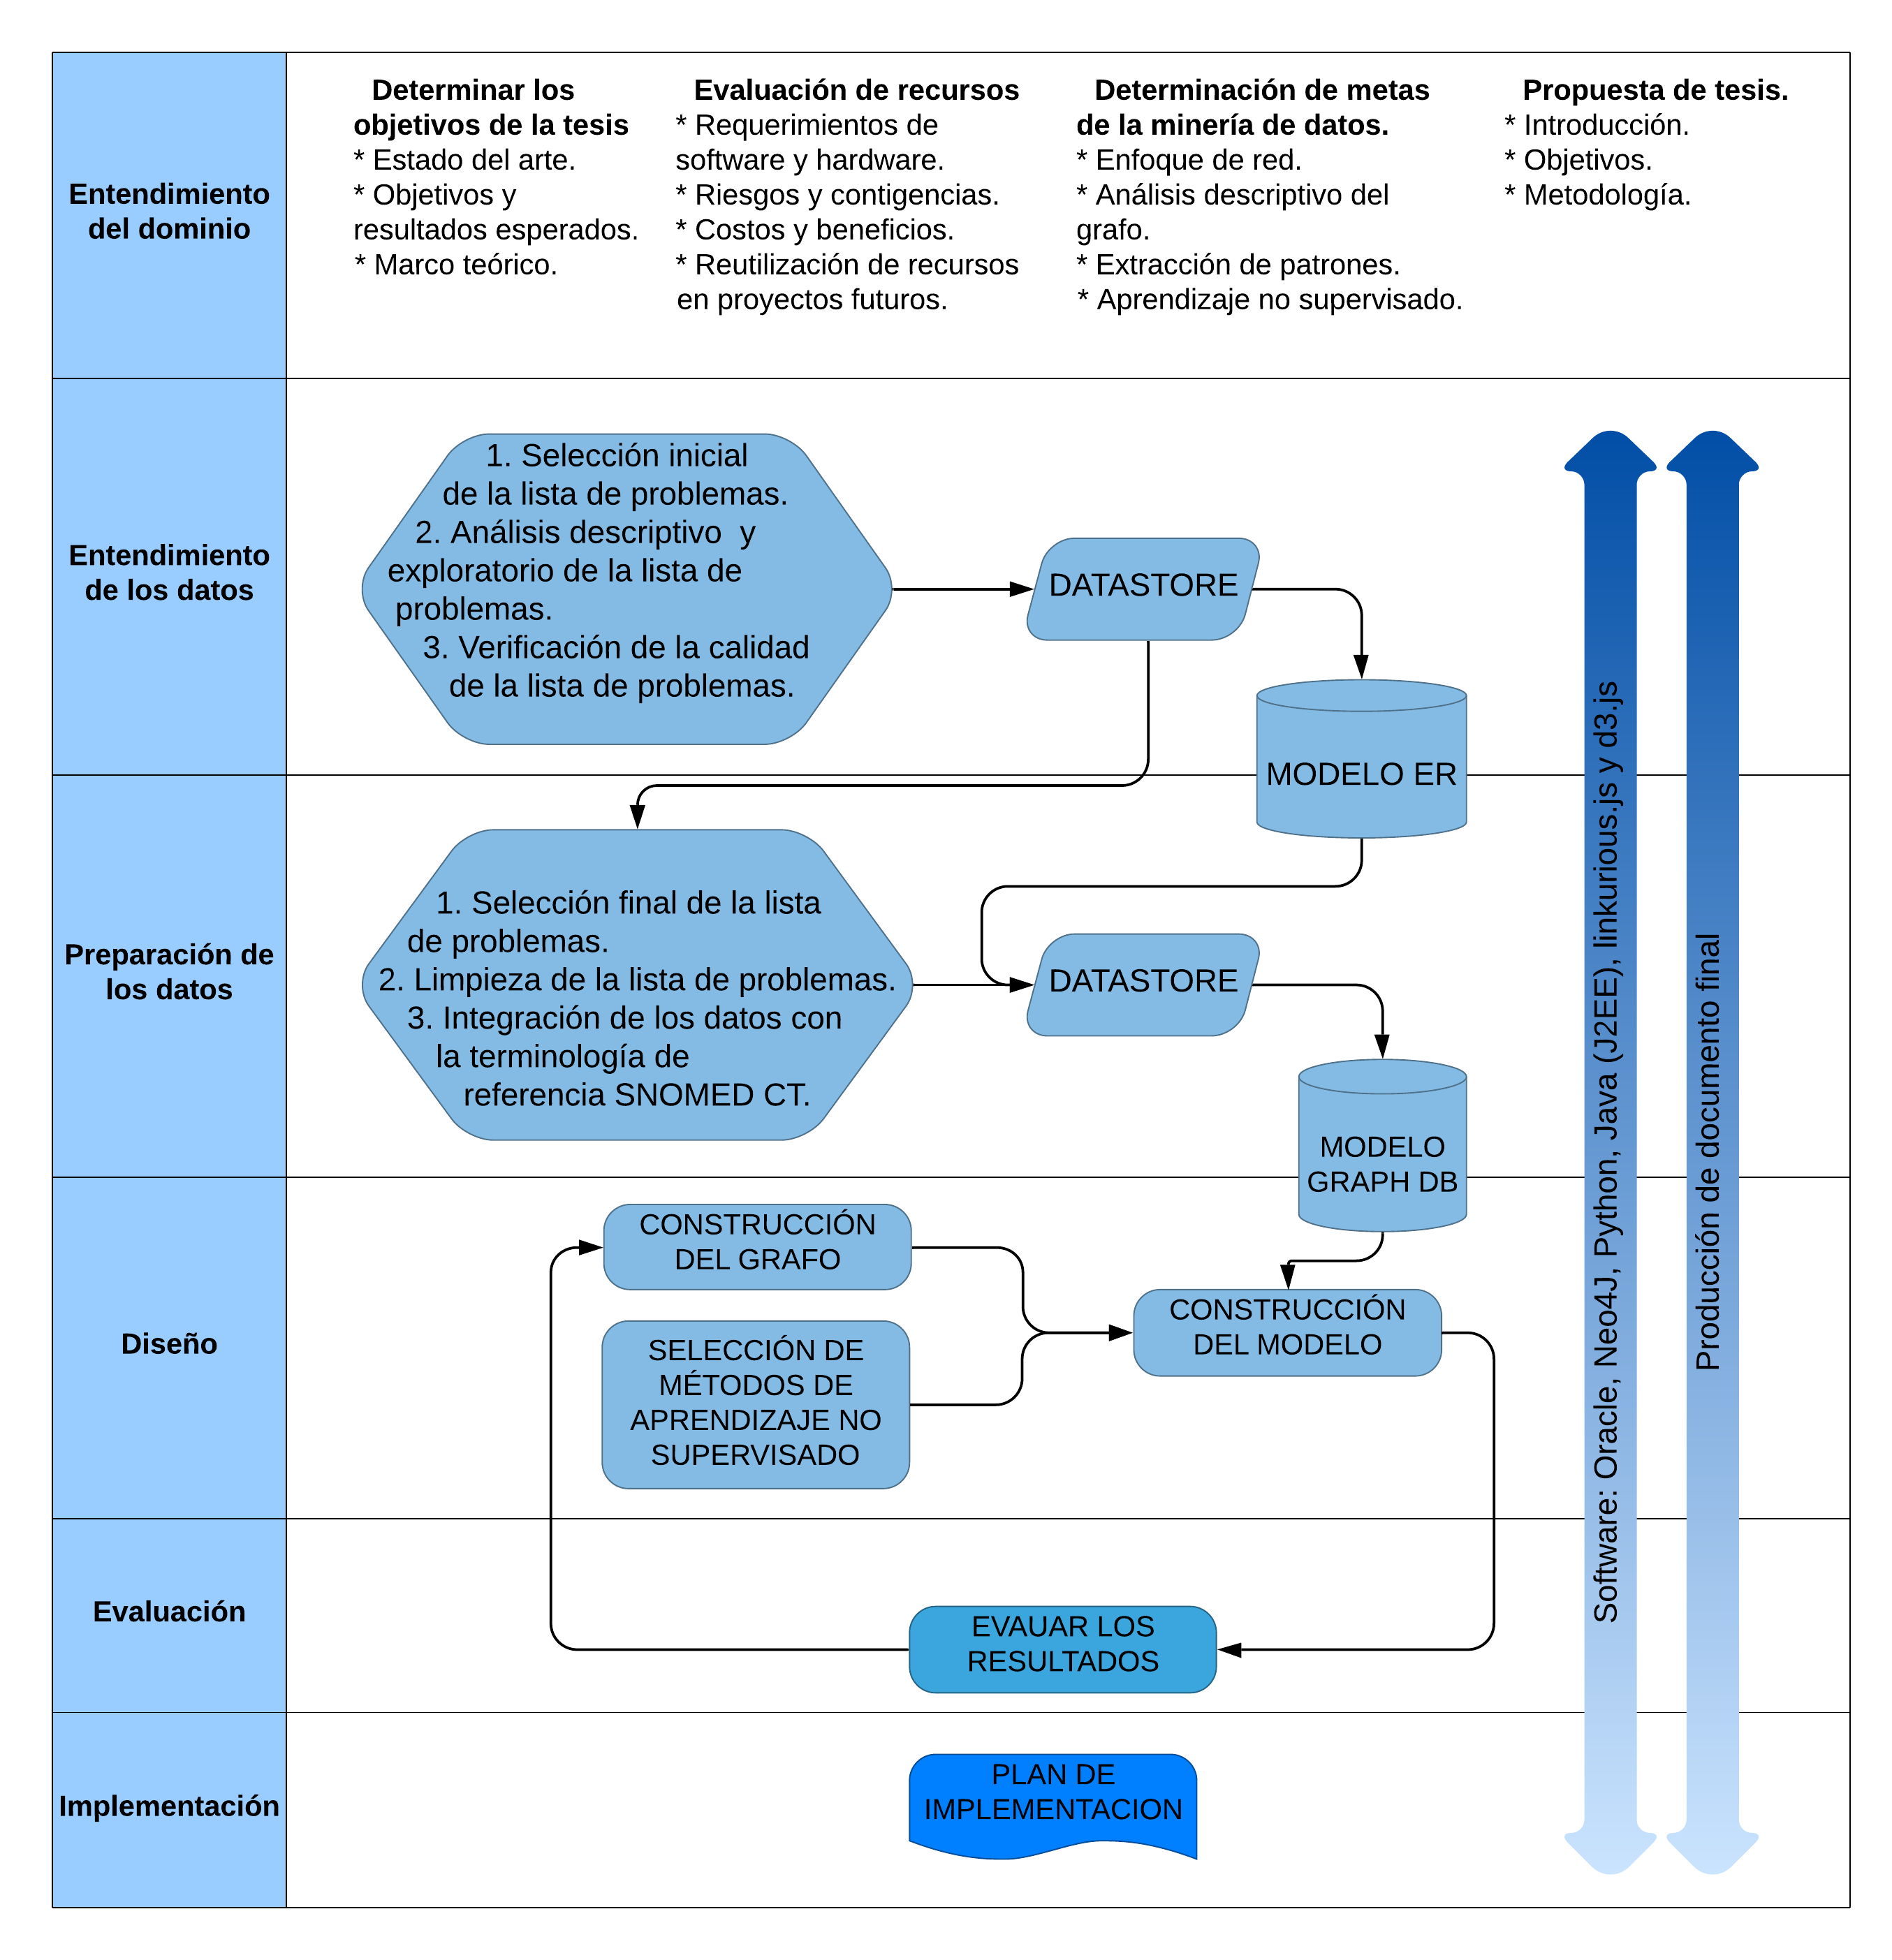
\includegraphics[width=\textwidth]{Metodologia}
\end{figure}

\subsection{Fase 1: Entendimiento del Dominio.} Esta fase fue previa al trabajo de tesis en sí, y el entregable fue la propuesta de tesis. Se compone de la determinación de los objetivos, de las metas de minería de datos y la evaluación de los recursos.

Como está consignado en el primer capítulo introductorio, el objetivo es la construcción de una taxonomía de problemas, cuyas relaciones están ponderadas por su co-ocurrencia en las listas de problemas de los pacientes y sus relaciones jerárquicas con Snomed CT. Para alcanzar dicho objetivo, establecí que la meta de minería de datos es representar el conocimiento en un enfoque de red, y a partir del análisis de la red realizar la construcción jerárquica de grupos o clasificaciones de los problemas.

Para realizar esta tesis, el \acrshort{HIBA} proporcionó el acceso a los datos de la lista de problemas y la terminología Snomed CT. En términos de hardware, el \acrshort{HIBA} proporcionó el acceso a un servidor con las siguientes características:
\begin{itemize}
\item Sistema Operativo: Ubuntu 16.04.5 LTS (GNU/Linux 4.4.0-138-generic x86\_64)
\item Memoria RAM: 64 GB 
\item Espacio de almacenamiento: 760 GB
\item Número de núcleos: 8 núcleos
\end{itemize}

\subsection{Fase 2: Entendimiento de los datos.} \label{par:entendimiento_datos} Esta fase inicia con la recolección de los datos y procede con las actividades que permitan familiarizarse con ellos. El entregable se encuentra en la primera sección del capítulo 3 y contempla un análisis descriptivo para determinar la calidad de los datos de la lista de problemas, la existencia de valores atípicos (\textit{outliers})  que deben ser eliminados de los datos de entrenamiento y validación, y la construcción de contextos interesantes que permitan la formulación de hipótesis.

La construcción de  \textit{\acrshort{refset}} para agrupar problemas por contextos tiene dos metodologías: (1) determinar por extensión cuáles son los conceptos que los componen. Ya que no es fácil hacerlo por comprensión usando las relaciones subtipo de Snomed CT.  \cite{Hjen2014MethodsSets.,Lee2013AImplementations.}; o (2) El uso de \textit{\acrshort{refset}} públicos para comparar el cubrimiento  con los \textit{\acrshort{refset}} generados aquí \cite{Lee2013AImplementations.}. Esta tesis usa la segunda metodología. Se usa aprendizaje no supervisado para generar grupos con los registros en la lista de problemas y los contextos en los cuales se realizaron los registros.  Si hay solapamiento de conceptos entre los contextos, se fusionan los contextos. Finalmente si hay \textit{\acrshort{refset}} similares en Kaiser Permanente \acrshort{CMT} entonces se evalúa el cubrimiento con ellos (Ver sección \ref{par:cubrimiento}).  Posteriormente las decisiones finales sobre fusión de  contextos son evaluados manualmente por la residencia de informática médica.  

Los contextos nivel asistencial y grupo etário tienen una cardinalidad pequeña, 8 y 9 respectivamente. Por el contrario, las áreas jerárquicas tienen una cardinalidad grande, inicialmente son 601 áreas jerárquicas. Las áreas jerárquicas tienen un proceso extra para evaluar sus solapamientos y así agruparlas dentro de las más significativas. Este último proceso se realiza con el algoritmo de aprendizaje supervisado StanfordNLP ColumnClassifier \cite{manning-EtAl:2014:P14-5}. La variable objetivo del algoritmo de clasificación es  el servicio al que pertenecen los conceptos, un algoritmo de clasificación tendría mayor dificultad para predecir el servicio si hay muchos conceptos similares entre ellos, por lo tanto serían candidatos a fusión. La dificultad se mide con valores de \textit{F1 score}\footnote{\textit{F1-Score} es un valor único que pondera la precisión y la exhaustividad. \textit{F1 score} hace referencia a la efectividad de un modelo y es conocida en la estadística como una proporción de acuerdo específico ya que se aplica a una clase específica, la clase positiva.\cite{Powers2011Evaluation:Correlation}} bajos. La residencia de informática médica determina manualmente si concuerda con la fusión de los contextos.


\subsection{Fase 3: Preparación de los datos.} Esta fase se compone de la extracción de los datos desde el modelo ER, limpieza y transformación de los datos con los que se realizan los modelos. El entregable es el conjunto de datos de entrenamiento y validación. El conjunto de entrenamiento contiene los registros de problemas previos al 2017. El conjunto de validación contiene los registros que ingresaron a la \acrshort{HCE} en el 2017 y cuyos pacientes tengan una lista de problemas no vacía.

\subsection{Fase 4 y 5: Diseño y evaluación.} \label{par:disenho_evaluacion} Esta fase se compone de las siguientes tareas:
\begin{itemize}
\item Construcción del grafo: Determinación del modelo de datos y carga de la base de datos de grafos Neo4j. Usando los datos de entrenamiento se obtiene un grafo cuyos vértices son los problemas y las aristas son las co-ocurrencias en los pacientes (Red de Problemas) y las relaciones dadas por la terminología de referencia Snomed CT (Red semántica de problemas). Los vértices son etiquetados con información contextual: ámbito o nivel de asistencia, grupo etario y área jerárquica.  

\item Caracterización de las redes y búsqueda de patrones en las redes:
\begin{itemize}
\item Determinar si la distribución de la red es libre de escala: La hipótesis nula es que la los grados de los vértices se distribuyen según la ley de potencias. Se estima la función de distribución acumulativa \acrshort{cdf}, en el caso de que el p-valor de la función no permita rechazar la hipótesis nula entonces se compara el estadístico \textit{log-likelihood ratio} con otras distribuciones.
\item Análisis de estructuras de comunidad: Métricas para comparar cuantitativamente los grafos de la red de problemas y la red semántica de problemas. Se evalúa si los grafos presenta evidencias de tener comunidades: coeficientes de agrupamiento, longitud media del camino mínimo entre nodos y promedio de grados. El cálculo de estas métricas están disponibles en los paquetes igraph\cite{igraph} y networkx\cite{SciPyProceedings_11} de python.
\end{itemize}

\item Aprendizaje no supervisado: Aplicación de algoritmos de aprendizaje no supervisado a la red de problemas y la red semántica de problemas. Por las limitaciones en hardware no se puede procesar el grafo completo de la red semántica de problemas, se realizan las siguientes tareas con sub-grafos de problemas que co-ocurran en \num{10000}, \num{1000}, \num{100}, \num{10} y \num{5} pacientes:
\begin{itemize}
    \item Identificación de grupos o \textit{clusters} significativos que comparten patrones comunes de atributos y relaciones. 
    \item Cada uno de los vértices que contiene el \textit{cluster} tiene calculada las medidas de centralidad para entender su influencia dentro de la red. 
    \item A los grupos encontrados se les realiza un test para evaluar la significancia de los \textit{clusters}, los siguientes pasos son realizados 1000 veces:
    \begin{itemize}
\item  se generan aleatoriamente aristas en el grafo
\item  se aplican los algoritmos de aprendizaje no supervisado
\item  se evalúa si la modularidad es superior a la modularidad del grafo original.
\end{itemize}
\end{itemize}

\item Validación de los resultados: 
\label{par:evaluacion-resultados}
Teniendo en cuenta las directrices de recuperación de información \cite{Manning2008IntroductionRetrieval,Hersh1994OHSUMED:Research}, el conjunto de validación tiene tres componentes: 

\begin{itemize}
\item \textbf{El conjunto de pruebas}: se conforma de los problemas registrados previamente y los valores del contexto (nivel asistencia, grupo etario y área jerárquica), que representan la consulta, y el problema a predecir que representa la respuesta correcta
\item \textbf{Los conceptos de Snomed CT a ser recuperados}: la lista previa de problemas permite identificar los subgrafos, y los valores de contexto permiten filtrar los vértices. De esta manera, creo una \textbf{lista de sugerencias} por cada uno de los registros del conjunto de pruebas.
\item una medida de relevancia por cada par de consulta-concepto recuperado, esta medida es la \textbf{transitividad} o la \textbf{distancia semántica}, y permite un ordenamiento de los resultados. Estas medidas están definidas en el capítulo introductorio (Ver sección \ref{par:efecto-comunidades}).
\end{itemize}

Lo que se evalúa es si los vértices que pertenecen al mismo \textit{cluster} permiten completar los problemas faltantes en la lista de los problemas de los pacientes del conjunto de datos de validación. Esta evaluación se realiza con la lista de problemas previas al 2017 y los contextos para seleccionar y filtrar la  \textbf{lista de sugerencias}, y predecir los problemas registrados en el 2017.

Se evalúan por separado la capacidad predictiva(Precisión y exactitud) de los grupos encontrados a partir del grafo de la red de problemas y del grafo de la red semántica de problemas. También son evaluadas las capacidades predictivas filtrando el contexto: ámbito o nivel de asistencia, grupo etario y área jerárquica, sólo en red de problemas. La precisión y la exactitud (\textit{accuracy}) se definen como:

\begin{equation}
Exactitud = \frac{\text{Verdaderos positivos}+\text{Verdaderos negativos}}{\text{Total de los datos}}
\end{equation}

\begin{equation}
Precision = \frac{\text{Verdaderos positivos}}{\text{Verdaderos positivos}+\text{Falsos positivos}}
\end{equation}

La exactitud suma los verdaderos positivos, que son los casos en los que la lista de sugerencia contiene la respuesta correcta, y los verdaderos negativos, que son los casos en los que la lista de sugerencias esta vacía y el problema a predecir no está dentro de los conceptos de Snomed CT a ser recuperados, y los divide en la totalidad de los datos de prueba. Se evalúa también una versión más flexible de verdadero positivo, donde se define una distancia tolerable de longitud media del camino mínimo entre la respuesta correcta y alguno de los conceptos de la lista de sugerencias. Esta distancia se estable de tamaño 3, e indica similitudes entre un concepto y los descendientes que están hasta dos vértices de distancia, o conceptos descendientes del mismo padre, como se ilustra en la figura \ref{fig:distancias_semanticas}.
 
La precisión evalúa cuántas veces la lista de sugerencias no vacía tiene la respuesta correcta, dividido las veces que se obtuvo una respuesta positiva. Teniendo en cuenta que las listas de sugerencias son de un tamaño $n$ ordenados según la relevancia, las medidas son llamadas precisión al $n$ o $P@n$ y exactitud al $n$ o $Acc@n$.

 \end{itemize}
 
\subsection{Fase 6: Implementación.} En la última fase organizo los datos y redacto el documento final de la tesis. El plan de implementación en la organización de los datos y los servicios de terminología del \acrshort{HIBA} no hacen parte de los entregables de esta tesis.






\chapter{Capítulo: Resultados de la descripción y limpieza de datos}
%%%% Resultados Parte 1
\section{Introducción}
Dentro de las fases para el desarrollo de un proyecto de minería de datos, después del entendimiento del dominio, se encuentra el entendimiento de los datos. Este capítulo se enmarca en el entendimiento de los datos y describe los resultados producto de las 3 actividades siguientes: (1) descripción de la lista de problemas desde cada una de las dimensiones de estudio (paciente, fecha de registro, problema cargado, área jerárquica del especialista, grupo etario del paciente y nivel de asistencia) (2) detección de valores atípicos y y (3) construcción de grupos de problemas según el contexto. 

Las dos primeras actividades permiten determinar la calidad de los datos y definir los criterios para la construcción del conjunto de entrenamiento y validación. En la tercera actividad creo \textit{\acrshort{refset}} que pueden ser utilizados como vocabularios controlados dependientes de contextos.

Transversalmente a todas las actividades realicé procesos de \acrfull{ETL}(Por su denominación en inglés: Extract, Transform and Load). Estos procesos tienen el objetivo de reducir la cardinalidad de algunas de las dimensiones mencionadas y permitir la interoperabilidad de los datos, de esta manera facilitar su posterior comparación con los realizados en otras instituciones.

\section{Comprensión de datos}
La lista de problemas registra las observaciones y hallazgos realizados a los pacientes y otra informacion del contexto. Los problemas de los pacientes son descripciones que se agrupan en conceptos, y los conceptos a su vez pertenecen a uno o varios \textit{\acrshort{refset}}.

Cualquier usuario con acceso a la \acrshort{HCE} puede registrar un problema, este usuario puede pertenece a una área administrativa o asistencial del \acrshort{HIBA}. Algunas de las áreas tienen sub-áreas, presentando así una estructura jerárquica. Cuando se registra un problema, se asocia el área jerárquica del que registra.

Además cada registro tiene el atributo nivel de asistencia que indica el ámbito en el que fue cargado el problema (1 = Ambulatorio , 2 = Internacion General, 3 = Guardia, 4 = Triage, 5 = Internacion Geriatrica, 6 = Internacion Domiciliaria, 7 = Seguimiento Domiciliario, 8 = Episodio Externo, 9 = Episodio Ambulatorio). La figura \ref{fig:ModeloER} contiene el modelo entidad relación, donde se muestra cómo se relacionan estos datos.

\begin{figure}[t]
\caption{Modelo Entidad-Relación de lista de problemas}
\label{fig:ModeloER}
\centering
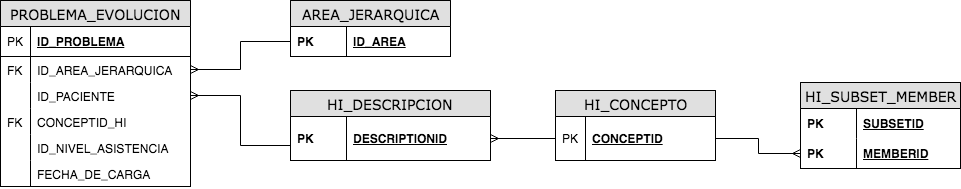
\includegraphics[width=0.9\textwidth]{ER_Problemas}
\end{figure}

Analizo a continuación la distribución de los problemas por cada una de las dimensiones de la entidad PROBLEMA\_EVOLUCION. 
 
\subsection{Distribución en el tiempo}
El atributo FECHA\_DE\_CARGA indica la fecha en la que se cargó el problema por primera vez. Las posteriores veces se vuelve a usar el problema registrado y no se crea uno nuevo. En la figura \ref{fig:registrosYConceptos}, se puede observar que aunque la implementación de la HCE empezó en el año 1998, hay registros anteriores a esa fecha, los cuales se interpretan como errores en el momento de la carga, al igual que los registros con las fechas superiores al 2017. En total son \num{9149} casos que corresponden al \num{0,004}\% de los datos.

Como se muestra en la figura \ref{fig:registrosYConceptos} la distribución no es uniforme, su crecimiento se explica por los hitos de implementación dentro de la HC, en el año \num{2002} se generalizó el uso de la HCE en todo el hospital, y en el año \num{2006} se implementó el servidor de terminología. Los años \num{2015} y \num{2016} muestran un incremento en el registro de la lista de problemas.

En cuanto a los conceptos diferentes registrados por año, se observa una distribución más uniforme, especialmente después del año \num{2007}. Los datos del año 2017 son sólo los del primer semestre.

\begin{figure}[tbp]
\caption{Distribución de problemas por año de carga}
\label{fig:registrosYConceptos}
\centering
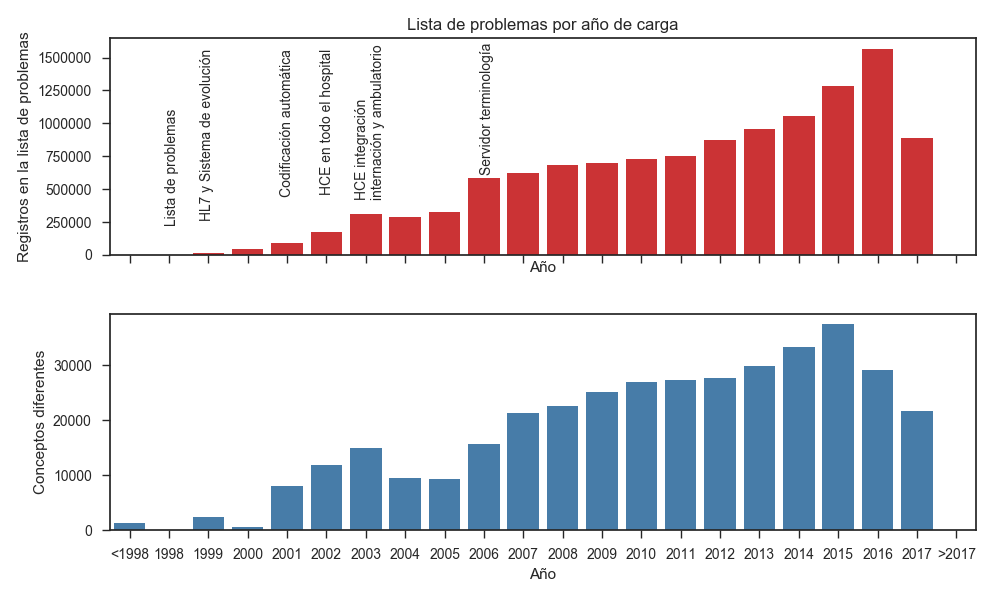
\includegraphics[width=\textwidth]{chart1}
\end{figure}

\subsection{Distribución por individuo}
Según la figura \ref{fig:listaIndividuos} la mayoría de los individuos tiene sólo un problema registrado en su lista de problemas, estos corresponde al \num{34.1}\% de los datos. Los individuos que tienen registrados hasta 10 problemas en la lista son el \num{80}\% de los datos.

\begin{figure}[t]
\caption{Distribución del tamaño de la lista de problemas por individuos}
\label{fig:listaIndividuos}
\centering
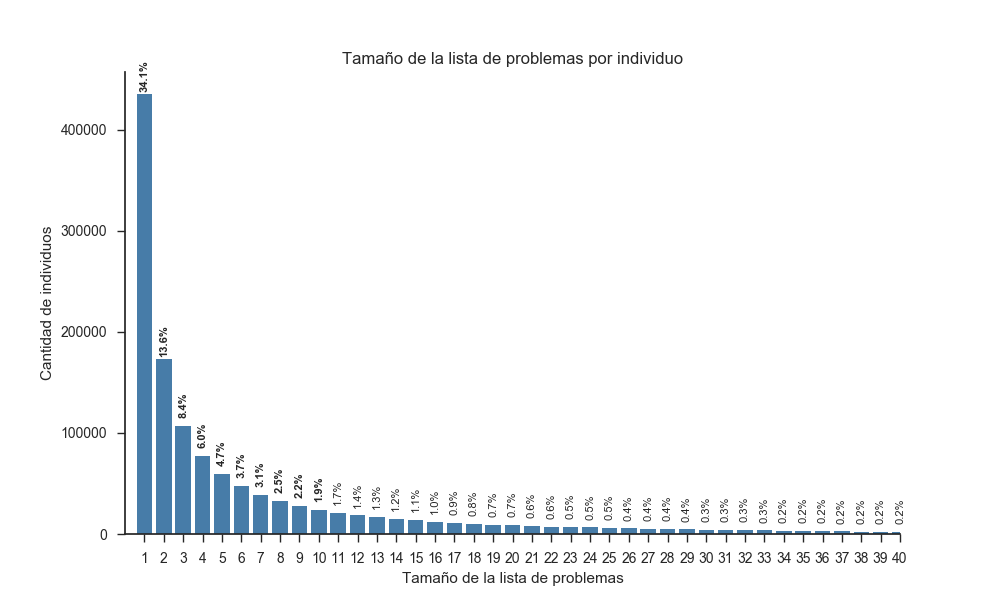
\includegraphics[width=\textwidth]{chart2}
\end{figure}

\subsection{Distribución por conceptos}
El conjunto de datos contiene \num{88869} conceptos distintos usados para identificar problemas de los pacientes. La figura \ref{fig:listaProblemas} representa el uso de estos conceptos en todos los registros de la lista de problemas, en ella se observa que un conjunto pequeño de problemas tiene una frecuencia muy alta y el resto que queda en la cola de la distribución son usados muy pocas veces. Los conceptos más frecuentemente usados son Control de salud, Fiebre, Dolor abdominal,  Hipertensión arterial, Catarro de las vías áreas superiores, Malestar general, Tos, Embarazo, Lumbalgia, Broncoespasmo, Evaluación inicial del paciente e Infección del tracto urinario, que juntos son el \num{20}\% del total de registros. 

\begin{figure}[t]
\caption{Distribución de todos los problema por su aparición en la lista}
\label{fig:listaProblemas}
\centering
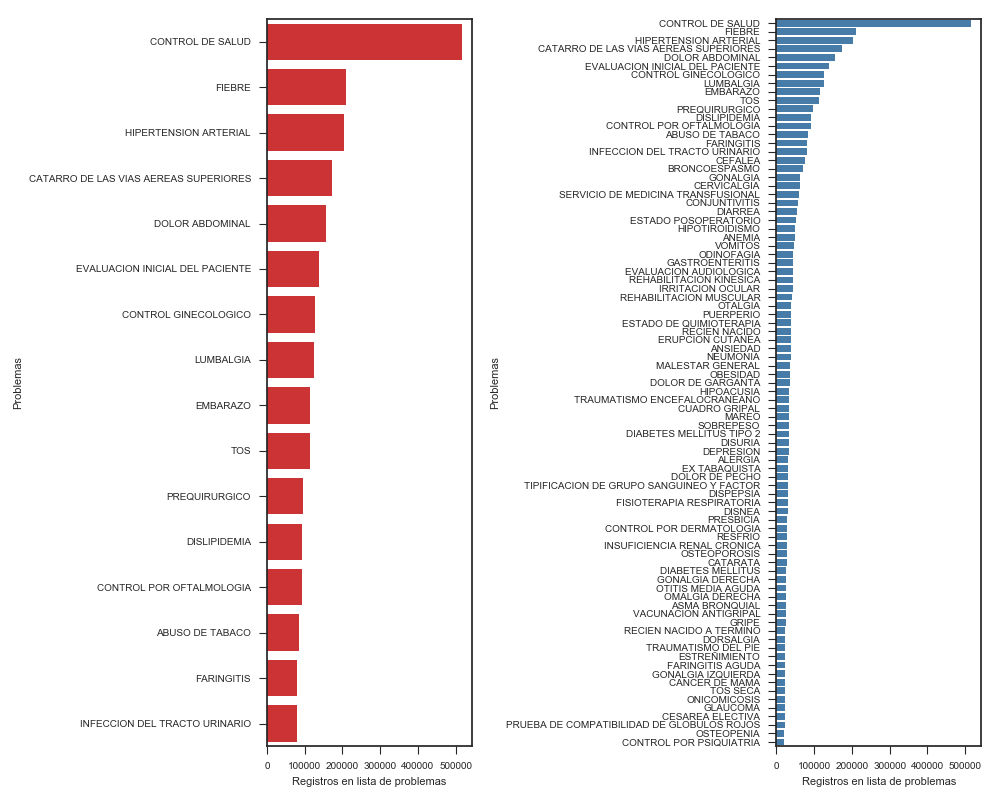
\includegraphics[width=\textwidth]{chart3}
\end{figure}

\subsection{Distribución por contextos}

Los contextos que tuve en cuenta en esta tesis fueron área jerárquica, nivel de asistencia y grupo etario, a continuación describo cómo se distribuyen los conceptos y registros de la lista de problemas en los contextos.

\subsubsection{Contexto: Área Jerárquica}
La \acrshort{HCE} tiene 918 áreas jerárquicas, de las cuales 601 tienen usuarios que han registraron problemas dentro de la lista de algún paciente. Hay dos jerarquías que usan más de \num{20000} conceptos (Clínica médica y Medicina Familiar), el resto de jerarquías usan en promedio menos de 5000 conceptos. (Ver figura XXXX)

Las áreas jerárquicas que tiene el \acrshort{HIBA} responden a necesidades operativas de la \acrshort{HCE}, y tienen diferentes niveles de agregación, por ejemplo: Sección de neurocirugía vascular hace parte de una área más general llamada Servicio de neurocirugía. En la sección que corresponde a la creación de los contextos, se evaluará si los datos de la lista de problemas necesitan también de ese nivel de detalle, o si las áreas pueden ser agrupadas de manera significativa. 

\subsubsection{Contexto: Nivel de asistencia}
Los niveles de asistencia son las diferentes modalidades de contacto que tiene el paciente con el hospital, asegurando una óptima atención en cada situación específica. En la \acrshort{HCE} el nivel de asistencia puede ser cualquier de los siguientes valores:

\begin{itemize}
\item Ambulatorio: Se tiene definido cuándo empieza y cuándo termina esa atención. El paciente solicita previamente un turno ambulatorio.
\item Episodio ambulatorio: Se sabe cuándo empieza pero no cuándo termina; entonces la modalidad de registro cambia. En el ambulatorio generalmente hay alguien que longitudinalmente ve al paciente en distintos momentos.
\item Triage: Se genera cuando un paciente tiene un contacto con el hospital sin un turno previo, consiste en una revisión médica rápida que permite definir la prioridad de atención.
\item Guardia: Los pacientes críticos con inminencia de muerte o que ingresa con una patología aguda de moderada o severa gravedad pero sin muerte inminente por la misma. El alta se da entre las 24 y 36 hs de su ingreso pudiendo trasladarse a otro nivel asistencial del hospital, o a otro hospital, o más rara vez a su domicilio.
\item Internación: Tiene un periodo limitado del cuidado, el paciente es tratado por un episodio grave de una enfermedad, cuyas condiciones puedan resultar en un trauma o su muerte. Los tipos de internación son general, domiciliaria y geriátrica.
\end{itemize}

Según la tabla \ref{nivel_asistencia} se puede observar que en 4 niveles de asistencia (Ambulatorio, Guardia, Triage e Internación general) están el 97\% del total de los registros de la lista de problemas. De estos 4 niveles de asistencia, en el caso de Ambulatoria y Guardia hay una relación en la que por cada 10 registros hay 1 concepto de Snomed CT diferente asociado a la lista de problemas, Triage es la relación más baja ya que es 20:1 entre los registros y los conceptos de Snomed  CT, e Internación General es la más alta (10:2).

\begin{table}[tb]
\centering
\caption{Distribución de registros y conceptos por nivel de asistencia o ámbito }
\label{nivel_asistencia}
\begin{tabular}{@{}lrrr@{}}
\toprule
Nivel de Asistencia o ámbito & Registros & Diferentes Conceptos \\ \midrule
Ambulatorio & \num{771096} & \num{9543} \\
Guardia & \num{603412} & \num{5759} \\
Triage & \num{556166} & \num{2963} \\
Internación general & \num{267303} & \num{6322} \\
Internación domiciliaria & \num{22297} & \num{1975}\\
Episodio ambulatorio & \num{17947} & \num{1247} \\
Seguimiento domiciliario & \num{14537} & \num{1302} \\
Internación geriátrica & \num{204} & \num{115} \\ \bottomrule
\end{tabular}
\end{table}

\subsubsection{Contexto: Grupo etario}
La distribución de los problemas registrados por edad en la figura \ref{fig:listaEdad} evidencia que los grupos etarios en los que más se consulta son 0-4 años, 25-34 años y mayores de 75 años.

\begin{figure}[t]
\caption{Distribución de todos los problema por edad de los pacientes}
\label{fig:listaEdad}
\centering
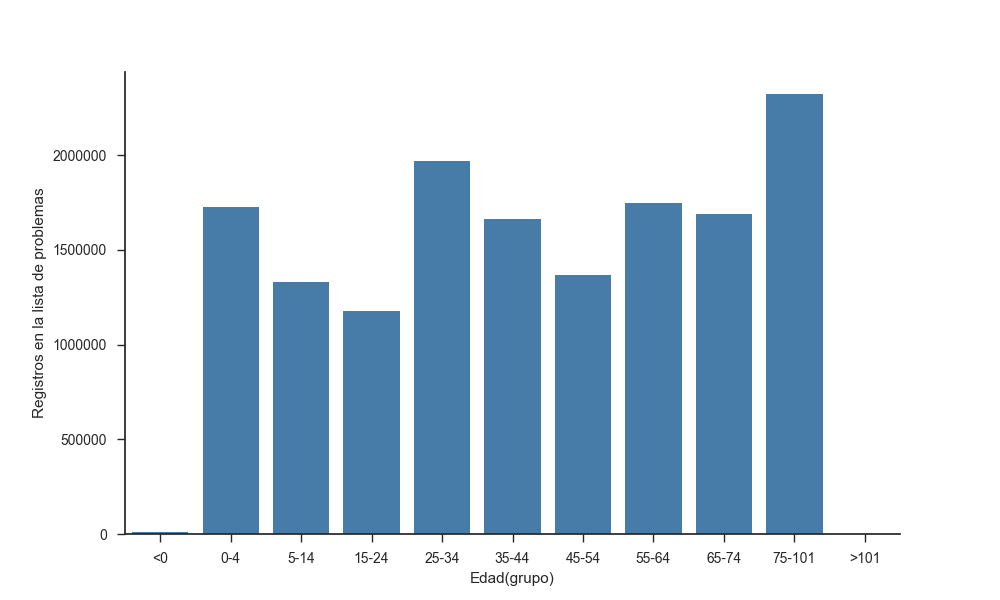
\includegraphics[width=\textwidth]{chart4}
\end{figure}

\subsubsection{Contexto: Área Jerárquica}

Para la construcción de estos \textit{refsets} se siguen dos metodologías, determinar por extensión cuáles son los conceptos que los componen, ya que no es fácil realizar la restricción por una jerarquía o partes de ella \cite{Hjen2014MethodsSets.,Lee2013AImplementations.}; o la generación automática y el uso de \textit{refsets} públicos para comparar el cubrimiento de su contenido \cite{Lee2013AImplementations.}. Este tesis usa la segunda metodología y evalúa el cubrimiento con Kaiser Permanente CMT.

La HCE tiene 918 áreas jerárquicas, de las cuales 601 tienen usuarios que han registraron problemas dentro de la lista de algún paciente. Hay dos jerarquías que usan más de \num{20000} conceptos (Clínica médica y Medicina Familiar), el resto de jerarquías usan en promedio menos de 5000 conceptos. 

Las áreas jerárquicas que tiene el HIBA responden a necesidades operativas de la HCE, pero su nivel de disgregación no significa que la lista de problemas necesite también ese nivel de detalle, por el contrario se evidencia al aplicar algoritmos de agrupamiento que hay solapamientos de jerarquías. Con el objetivo de reducir la cardinalidad en las áreas jerárquicas y agruparlas dentro de las más representativas e interoperables, seguí la metodología que se encuentra en la figura \ref{fig:MetodologiaReduccionAreas}.


\begin{figure}[ht]
\caption{Metodología para reducción de áreas jerárquicas}
\label{fig:MetodologiaReduccionAreas}
\centering
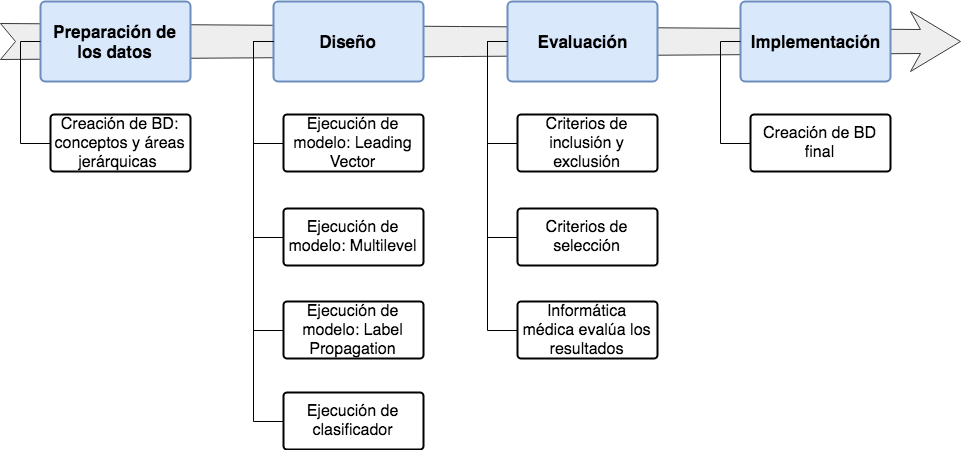
\includegraphics[width=0.9\textwidth]{Reducci_n_cardinalidad}
\end{figure}

En la primera fase de preparación de los datos, cree la base de datos de grafos. En el modelo de datos que se observa en la figura \ref{fig:ModeloDatosAreas} los nodos son los conceptos y las áreas jerárquicas, y las relaciones son las jerarquías (ES\_UN) entre los conceptos y su uso (REGISTRA\_PROBLEMA)  por el área. De tal manera que se represente los diferentes niveles de generalización de los conceptos con la relación (ES\_UN), y que un área jerárquica tiene varios conceptos y un concepto puede estar en varias áreas con la relación (REGISTRA\_PROBLEMA). 

\begin{figure}[ht]
\caption{Modelo de datos}
\label{fig:ModeloDatosAreas}
\centering
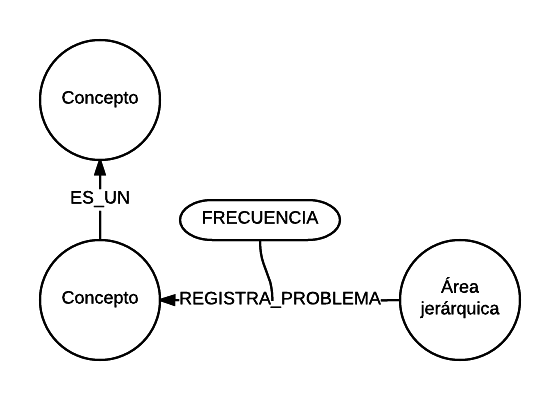
\includegraphics[width=0.5\textwidth]{Modelo_grafo_areas}
\end{figure}

La segunda fase tiene el propósito de encontrar qué áreas jerárquicas comparten similares conceptos, y así identificar las áreas que se pueden agrupar como una sola. En el segundo experimento el propósito es identificar los servicios que se están solapando entre sí, usé un algoritmo de aprendizaje supervisado para predecir el servicio al que pertenecen los conceptos, este algoritmo tiene mayor dificultad para predecir el servicio si hay muchos conceptos similares entre ellos por lo tanto serían candidatos a fusión.

La tercera fase es para evaluar el modelo, se compone de:(a) Informáticos médicos determinan si los criterios se deben aplicar a cada una de las 918 áreas, y (b) Evaluación de la cobertura de los \textit{refsets} formados a partir de los servicios finales.

\paragraph{Fase de diseño:Experimento 1 (Agrupamiento de áreas jerárquicas)}

\subparagraph{Criterios de exclusión}

\begin{itemize}
\item Áreas jerárquicas con sólo un concepto seleccionado.
\item Áreas jerárquicas dentro del cluster de administrativos, las cuales corresponden a usuarios que seleccionaron problemas por razones operativas administrativas y no por razones médicas.
\end{itemize}

\subparagraph{Criterios de selección}
\begin{itemize}
\item Los servicios de la atención de la salud de la jerarquía de SNOMED CT son usados para mapear los del HIBA, de tal manera que los servicios finales permitan la interoperabilidad con otros centros de salud. Para realizar el mapeo, hice una búsqueda en SNOMED CT con string matching del nombre del área del HIBA o del área más general que la contenía.
\item Si no hay un mapeo, seleccioné el servicio de las áreas que están dentro del mismo cluster de label propagation y multilevel, y que además hayan seleccionado los mismos conceptos.
%\item Si al aplicar un algoritmo de clasificación se presenta un alto solapamiento de conceptos entre servicios, estos son candidatos a fusionarse
\end{itemize}

\subparagraph{Diseño del modelo}: Ejecuté 3 algoritmos de agrupamiento. como se observa en la tabla \ref{clusteringAreas}, el algoritmo leading vector dividió el conjunto de datos en 2 y su modularidad es la más baja por lo tanto sus resultados se descartaron.  Los resultados de los otros dos algoritmos fueron usados en los criterios de selección de jerarquía.

\begin{table}[htb]
\centering
\caption{Agrupamiento de áreas jerárquicas y conceptos}
\label{clusteringAreas}
\begin{tabular}{@{}llll@{}}
\toprule
Algoritmo         & Modularidad & Grupos & Test \\ \midrule
Label Propagation & 0.165       & 18     &      \\
Leading Vector    & 0.144       & 2      &      \\
MultiLevel        & 0.447       & 14     &      \\ \bottomrule
\end{tabular}
\end{table}

\paragraph{Fase de diseño:Experimento 2 (Clasificador de áreas jerárquicas)}

\subparagraph{Criterios de selección}
\begin{itemize}
\item Si al aplicar un algoritmo de clasificación se presenta un alto solapamiento de conceptos entre servicios, estos son candidatos a fusionarse
\end{itemize}

\subparagraph{Diseño del modelo}: 
Un enfoque de clasificación permite identificar aquellos servicios que tienen una superposición de conceptos. Usé el algoritmo de aprendizaje supervisado StanfordNLP ColumnClassifier \cite{manning-EtAl:2014:P14-5},  para predecir el servicio al que pertenecen los conceptos, este algoritmo tiene mayor dificultad al predecir el servicio si hay muchos conceptos similares entre ellos.

\paragraph{Evaluación final del modelo}: Ejemplos de los resultados de la aplicación de los criterios de exclusión y de selección del primer experimento se encuentran en la tabla \ref{ejemploCriterios}. Los resultados de la aceptación de estos criterios se encuentran en la tabla \ref{resultadosCriterios}, el \num{63}\% de los casos fueron excluidos correctamente. Con respecto a los criterios de selección, el \num{96}\% de los casos fueron seleccionados correctamente según la evaluación realizada por la residencia médica.

% Please add the following required packages to your document preamble:
% \usepackage{booktabs}
\begin{table}[htb]
\centering
\caption{Ejemplos de criterios de exclusión y selección}
\label{ejemploCriterios}
\begin{tabularx}{\textwidth}{@{}XlXX@{}}
\toprule
Área Jerárquica                                                          & Excluído? & Servicio Seleccionado            & Observaciones                                                     \\ \midrule
Dirección administrativa                                                 & Si        &                                  & Hace Parte Del Cluster De Administrativos                         \\
Coordinación de turnos - departamento de enfermería                      & Si        &                                  & Tiene un sólo concepto seleccionado.                              \\
Servicio de neurocirugía                                                 & No        & Servicio de neurocirugía         & \textit{String Matching} Con un servicio de Snomed CT                      \\
Sección diálisis peritoneal continua ambulatoria- Servicio de nefrología & No        & Servicio de nefrología adultos   & \textit{String Matching} del área más general con un servicio de Snomed CT \\
Rinología plástica                                                       & No        & servicio de otorrinolaringología & Comparte cluster con áreas con los mismos conceptos.              \\ \bottomrule
\end{tabularx}
\end{table}

% Please add the following required packages to your document preamble:
% \usepackage{booktabs}
\begin{table}[htb]
\centering
\caption{Resultados de la aplicación de los criterios de exclusión y selección}
\label{resultadosCriterios}
\begin{tabular}{@{}lll@{}}
\toprule
Criterio                      & Reportados & Aceptados \\ \midrule
Criterio de exclusión         & 223        & 142       \\
Selección por string matching & 291        & 291       \\
Selección por agrupamiento    & 116        & 111       \\ \bottomrule
\end{tabular}
\end{table}

En este primer experimento reemplacé las 601 áreas jerárquicas con 44 servicios de atención médica de SNOMED CT, y eliminé las que entraron en el criterio de exclusión y fueron aceptadas por el residente.

En el segundo experimento, los datos de entrada son los conceptos y los servicios finales del experimento 1. Realizando una partición de 50\% de los datos para crear entrenamiento y 50\% para test, el modelo creado predice a qué servicio pertenecen los conceptos, con los siguientes F1 score:  Accuracy/micro-averaged F1: 0.736, Macro-averaged F1: 0.500.

La matriz de confusión generada por el modelo aporta información sobre qué servicios comparten los mismos conceptos, y propone así una fusión entre ellos. La tabla \ref{serv_aten_hiba} contiene los 44 servicios que fueron mapeados en el experimento 1, y los 29 servicios finales obtenidos a partir del experimento 2. Al crear un nuevo modelo con los mapeos de los servicios del experimento 2, obtengo los siguientes F1 score: Accuracy/micro-averaged F1: 0.775, Macro-averaged F1:0.664

% Please add the following required packages to your document preamble:
% \usepackage{booktabs}
% \usepackage{graphicx}
\begin{table}[htb]
\centering
\caption{Servicios de atención médica del HIBA}
\label{serv_aten_hiba}
\resizebox{\textwidth}{!}{%
\begin{tabular}{@{}lrrlrrl@{}}
\toprule
Servicios Experimento 1 & F1 Score & TP & Servicios Experimento 2 & F1 Score & Solapados & Acción \\ \midrule
servicio de anestesia & 0,048 & 155 & servicio de medicina general & 0,747 & 1595 & Fusionar \\
servicio audiológico & 0,000 & 0 & servicio de otorrinolaringología & 0,675 & 10 & Fusionar \\
servicio de cardiología adultos & 0,672 & 29589 & servicio de cardiología adultos & 0,672 & - & Mantener \\
servicio de cardiología pediátrica & 0,871 & 9531 & servicio de cardiología pediátrica & 0,871 & - & Mantener \\
servicio de cirugía general & 0,598 & 29993 & servicio de cirugía general & 0,598 & - & Mantener \\
servicio de cirugía pediátrica & 0,437 & 3490 & servicio de cirugía pediátrica & 0,437 & - & Mantener \\
servicio de cirugía plástica & 0,664 & 3619 & servicio de cirugía plástica & 0,664 & - & Mantener \\
servicio de cirugía vascular & 0,178 & 406 & servicio de cardiología adultos & 0,672 & 909 & Fusionar \\
servicio de colposcopía & 0,000 & 0 & servicio de ginecoobstetricia & 0,877 & 293 & Fusionar \\
servicio de dermatología & 0,800 & 39370 & servicio de dermatología & 0,800 & - & Mantener \\
servicio de dermatología pediátrica & 0,405 & 2141 & servicio de dermatología & 0,800 & 3240 & Fusionar \\
servicio de endocrinología & 0,687 & 20509 & servicio de endocrinología & 0,687 & - & Mantener \\
servicio de endocrinología pediátrica & 0,518 & 1003 & servicio de endocrinología pediátrica & 0,518 & - & Mantener \\
servicio de enfermería & 0,595 & 5968 & servicio de enfermería & 0,595 & - & Mantener \\
servicio de farmacia & 0,392 & 112 & servicio de medicina general & 0,747 & 186 & Fusionar \\
servicio de fisioterapia & 0,993 & 34731 & servicio de fisioterapia & 0,993 & - & Mantener \\
servicio de fonoaudiología & 0,612 & 7402 & servicio de otorrinolaringología & 0,675 & 6136 & Fusionar \\
servicio de gastroenterología & 0,233 & 2716 & servicio de medicina general & 0,747 & 13836 & Fusionar \\
servicio de gastroenterología pediátrica & 0,000 & 0 & servicio de otorrinolaringología & 0,675 & 1 & Fusionar \\
servicio de ginecoobstetricia & 0,877 & 77215 & servicio de ginecoobstetricia & 0,877 & - & Mantener \\
servicio de hemoterapia & 0,686 & 374 & servicio de hemoterapia & 0,686 & - & Mantener \\
servicio de imagenología & 0,546 & 2198 & servicio de imagenología & 0,546 & - & Mantener \\
servicio de internacion domiciliaria & 0,131 & 15 & servicio de medicina general & 0,747 & 86 & Fusionar \\
servicio de medicina general & 0,747 & 390596 & servicio de medicina general & 0,747 & - & Mantener \\
servicio de nefrología adultos & 0,674 & 6950 & servicio de nefrología adultos & 0,674 & - & Mantener \\
servicio de neonatología & 0,682 & 11659 & servicio de neonatología & 0,682 & - & Mantener \\
servicio de neumología pediátrica & 0,622 & 1712 & servicio de neumología pediátrica & 0,622 & - & Mantener \\
servicio de neurocirugía & 0,400 & 1371 & servicio de neurocirugía & 0,400 & - & Mantener \\
servicio de neurología adultos & 0,432 & 7436 & servicio de neurología adultos & 0,432 & - & Mantener \\
servicio de neuropediatría & 0,566 & 3028 & servicio de neuropediatría & 0,566 & - & Mantener \\
servicio de odontología adultos & 0,900 & 796 & servicio de odontología adultos & 0,900 & - & Mantener \\
servicio de oftalmología adultos & 0,938 & 57983 & servicio de oftalmología adultos & 0,938 & - & Mantener \\
servicio de oncología clinica & 0,105 & 123 & servicio de oncología clinica & 0,105 & - & Mantener \\
servicio de otorrinolaringología & 0,675 & 24418 & servicio de otorrinolaringología & 0,675 & - & Mantener \\
servicio de patología & 0,000 & 0 & servicio de imagenología & 0,546 & 32 & Fusionar \\
servicio de pediatría & 0,243 & 7699 & servicio de pediatría & 0,243 & - & Mantener \\
servicio de psicología & 0,000 & 0 & servicio de psiquiatria & 0,827 & 32 & Fusionar \\
servicio de psiquiatria & 0,827 & 8268 & servicio de psiquiatria & 0,827 & - & Mantener \\
servicio de psiquiatria pediátrica & 0,945 & 4159 & servicio de psiquiatria pediátrica & 0,945 & - & Mantener \\
servicio de reumatología & 0,336 & 96 & servicio de medicina general & 0,747 & 226 & Fusionar \\
servicio de terapia intensiva & 0,275 & 968 & servicio de medicina general & 0,747 & 1725 & Fusionar \\
servicio de terapia intensiva pediátrica & 0,179 & 156 & servicio de medicina general & 0,747 & 308 & Fusionar \\
servicio de traumatología & 0,821 & 143770 & servicio de traumatología & 0,821 & - & Mantener \\
servicio de urología & 0,678 & 15232 & servicio de urología & 0,678 & - & Mantener \\ \bottomrule
\end{tabular}%
}
\end{table}

El último nivel de evaluación lo realicé midiendo el cubrimiento de los servicios\cite{Yu2012ClinicalSNOMED-CT}, el cual está definido como la proporción de los conceptos que se comparten con un servicio, al tamaño del \textit{refset} de referencia, como se define en la ecuación \ref{eq:cubrimiento}
\begin{equation}\label{eq:cubrimiento}
\textup{cubrimiento} = \frac{\textup{conceptos mapeados en T}}{\textup{Tamaño de T}}
\end{equation}

\begin{itemize}
\item \textit{Conceptos mapeados en T}, es el número total de conceptos de Snomed CT que se comparten con el \textit{refset} de referencia $T$, y
\item el \textit{tamaño de T} es el número total de conceptos que tiene el \textit{refset} de referencia $T$.
\end{itemize}

La validación del cubrimiento de los servicios implican la comparación de los mismos con otros que ya estén avalados, para realizar esta comparación usé el conjunto de de términos llamados \textit{Convergent Medical Terminology (CMT) }construído por \textit{Kaiser Permanente}. La tabla \ref{subsetsComparacion} contiene los servicios que se compararon con \textit{CMT}, en algunos casos necesité unir varios servicios para comparar con uno sólo de \textit{CMT} como el caso de los servicios de nefrología de adultos, endocrinología, endocrinología pediátrica y urología que se unieron para comprar con el subset \textit{Endocrine, Nephrology, and Urology} de \textit{CMT}.

% Please add the following required packages to your document preamble:
% \usepackage{booktabs}
\begin{table}[htb]
\centering
\caption{Subsets afines entre de HIBA y CMT}
\label{subsetsComparacion}
\begin{tabularx}{\textwidth}{@{}XXl@{}}
\toprule
Servicio HIBA                                                                                                              & Subset Kaiser Permanente & Abreviatura                         \\ \midrule
servicio de cardiologia adultos +\newline  servicio de cardiologia pediatrica                                                       & Cardiology Problem List. Version 2016          & Cardio  \\
servicio de oftalmologia adultos                                                                                           & Ophthalmology Problem List. Version 2016        & Oftalmo \\
servicio de psiquiatria                                                                                                    & Mental Health Subset. Version 2016          & Psiqui     \\
servicio de oncologia clinica                                                                                              & Hematology and Oncology. Version 2015       & Onco     \\
servicio de nefrologia adultos +\newline  servicio de endocrinologia +\newline  servicio de endocrinologia pediatrica +\newline  servicio de urologia & Endocrine, Nephrology, and Urology. Version 2015  & ENU \\
servicio de ginecoobstetricia                                                                                              & Obstetrics and Gynecology. Version 2015        & Gineco  \\
servicio de neurocirugia + servicio de neuropediatria +\newline  servicio de neurologia adultos                                     & Neurology. Version 2015                & Neuro          \\
servicio de dermatologia                                                                                                   & Skin/Dermatology and Respiratory. Version 2015  &Derma  \\
servicio de pediatria                                                                                                      & Pediatrics. Version 2014                     & Pedia    \\
servicio de traumatologia                                                                                                  & Orthopedics. Version 2014                      & Orto  \\ \bottomrule
\end{tabularx}
\end{table}


La tabla \ref{kaiserPermanenteCubrimiento} muestra el cálculo de la cobertura de los \textit{refset} \textit{CMT} comparándolos con los servicios, se puede observar que las mayores coberturas se encuentran en los conjuntos de datos afines relacionados en la tabla \ref{subsetsComparacion}

% Please add the following required packages to your document preamble:
% \usepackage{booktabs}
% \usepackage{multirow}
\begin{table}[htb]
\centering
\caption{Cubrimiento de Kaiser Permanente en Servicios de HIBA}
\label{kaiserPermanenteCubrimiento}
\resizebox{\textwidth}{!}{%
\begin{tabular}{@{}lllllllllll@{}}
\toprule
\multirow{2}{*}{\textbf{Hiba (número de conceptos)}} & \multicolumn{10}{l}{\textbf{Kaiser permanente (número de conceptos)}}                                                                                                                                                                 \\ \cmidrule(l){2-11} 
                                                     & \textbf{Cardio (880)} & \textbf{Derma(2757)} & \textbf{Gineco(1307)} & \textbf{ENU(1639)} & \textbf{Neuro(1792)} & \textbf{Oftalmo(3285)} & \textbf{Onco(4086)} & \textbf{Pedia(3793)} & \textbf{Psiqui (1163)} & \textbf{Orto(5009)} \\ \cmidrule(r){1-1}
Cardio(9182)                                         & 0,46                  & 0,33                 & 0,11                  & 0,20               & 0,19                 & 0,09                   & 0,14                & 0,34                 & 0,13                   & 0,15                \\
Derma(11622)                                         & 0,14                  & 0,45                 & 0,08                  & 0,11               & 0,10                 & 0,06                   & 0,20                & 0,27                 & 0,08                   & 0,13                \\
Gineco(8319)                                         & 0,15                  & 0,18                 & 0,33                  & 0,16               & 0,09                 & 0,06                   & 0,11                & 0,27                 & 0,10                   & 0,11                \\
ENU(18075)                                           & 0,31                  & 0,42                 & 0,21                  & 0,40               & 0,42                 & 0,17                   & 0,22                & 0,46                 & 0,28                   & 0,24                \\
Neuro(10856)                                         & 0,26                  & 0,31                 & 0,13                  & 0,19               & 0,40                 & 0,16                   & 0,17                & 0,39                 & 0,26                   & 0,21                \\
Oftalmo (4188)                                       & 0,06                  & 0,06                 & 0,02                  & 0,04               & 0,10                 & 0,41                   & 0,03                & 0,16                 & 0,04                   & 0,09                \\
Onco (721)                                           & 0,07                  & 0,03                 & 0,02                  & 0,03               & 0,03                 & 0,00                   & 0,07                & 0,05                 & 0,02                   & 0,01                \\
Pedia (17325)                                        & 0,26                  & 0,31                 & 0,18                  & 0,27               & 0,25                 & 0,18                   & 0,18                & 0,56                 & 0,22                   & 0,28                \\
Psiqui(2373)                                         & 0,07                  & 0,13                 & 0,07                  & 0,06               & 0,08                 & 0,03                   & 0,03                & 0,16                 & 0,30                   & 0,07                \\
Orto(22555)                                          & 0,21                  & 0,37                 & 0,09                  & 0,13               & 0,24                 & 0,05                   & 0,16                & 0,34                 & 0,10                   & 0,42                \\ \bottomrule
\end{tabular}%
}
\end{table}

Los niveles de precisión entre los dos conjuntos de datos hace compleja la tarea de comparación. Por ejemplo, en el caso del \textit{refset} del servicio de cardiología del HIBA tenemos el hallazgo Ulcera Arterial, el cual no aparece en el \textit{refset} de cardiología de Kaiser Permanente, pero Ulcera Arterial es hijo de trastorno arterial, el cual es una generalización que si aparece en Kaiser Permanente. Por lo tanto, este término debió ser contado como parte de la cobertura.

Por lo tanto, calculé el cubrimiento con conceptos cuya longitud media del camino mínimo es \textless=1, \textless=2 y \textless=3. De esta manera entran en el conteo los conceptos hijos de un mismo ancestro, y con diferentes niveles de precisión, estas distancias están ilustradas en la figura \ref{fig:distancias_semanticas}. Esta medida es usada como distancia semántica en diferentes trabajos en el dominio médico\cite{Wang2010,Gan2013,Pedersen2007,Zare2015ASNOMED-CT}. Estos trabajos presentan maneras más sofisticadas de calcular la similaridad entre conceptos, y usan como base alguna variante de la longitud media del camino mínimo.

\begin{figure}[ht]
\caption{Modelo de datos}
\label{fig:distancias_semanticas}
\centering
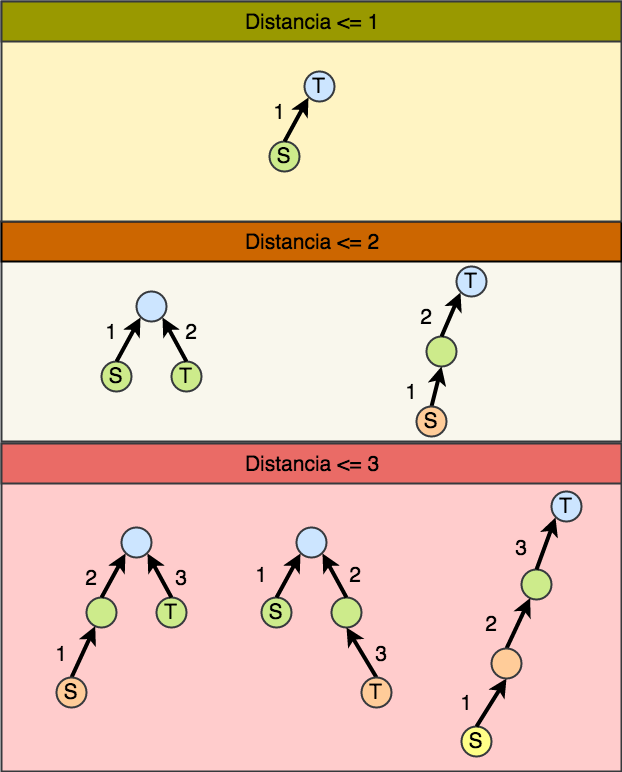
\includegraphics[width=0.5\textwidth]{distancias_semanticas}
\end{figure}

% Please add the following required packages to your document preamble:
% \usepackage{booktabs}
% \usepackage{multirow}
\begin{table}[htb]
\centering
\caption{Cubrimientos de servicios con distancias semánticas entre 1 y 3}
\label{cubrimiento_1y3}
\resizebox{\textwidth}{!}{%
\begin{tabular}{@{}lrrrrrrrr@{}}
\toprule
\multirow{2}{*}{Servicio} & \multicolumn{2}{l}{\begin{tabular}[c]{@{}l@{}}Cubrimientos con \\ Distancia Semántica \textless=3\end{tabular}} & \multicolumn{2}{l}{\begin{tabular}[c]{@{}l@{}}Cubrimientos con \\ Distancia Semántica \textless=2\end{tabular}} & \multicolumn{2}{l}{\begin{tabular}[c]{@{}l@{}}Cubrimientos con \\ Distancia Semántica \textless=1\end{tabular}} & \multicolumn{2}{l}{Cubrimientos exactos} \\ \cmidrule(l){2-9} 
 & Kaiser/Hiba & Hiba/Kaiser & Kaiser/Hiba & Hiba/Kaiser & Kaiser/Hiba & Hiba/Kaiser & Kaiser/Hiba & Hiba/Kaiser \\ \cmidrule(r){1-9}
Cardio & 0,475 & 0,947 & 0,320 & 0,890 & 0,211 & 0,782 & 0,104 & 0,457 \\
Oftalmo & 0,779 & 0,969 & 0,647 & 0,949 & 0,505 & 0,787 & 0,257 & 0,407 \\
Derma & 0,831 & 0,974 & 0,683 & 0,942 & 0,452 & 0,824 & 0,242 & 0,449 \\
Pedia & 0,85 & 0,973 & 0,769 & 0,940 & 0,594 & 0,857 & 0,305 & 0,560 \\
ENU & 0,492 & 0,979 & 0,319 & 0,944 & 0,174 & 0,811 & 0,075 & 0,403 \\
Onco & 0,582 & 0,879 & 0,433 & 0,623 & 0,307 & 0,252 & 0,073 & 0,173 \\
Psiqui & 0,572 & 0,904 & 0,476 & 0,813 & 0,384 & 0,627 & 0,227 & 0,303 \\
Orto & 0,726 & 0,986 & 0,586 & 0,963 & 0,402 & 0,860 & 0,179 & 0,420 \\
Neuro & 0,563 & 0,975 & 0,385 & 0,963 & 0,227 & 0,825 & 0,112 & 0,404 \\
Gineco & 0,597 & 0,936 & 0,443 & 0,904 & 0,284 & 0,743 & 0,119 & 0,326 \\ \bottomrule
\end{tabular}%
}
\end{table}

Como se muestra en la tabla \ref{cubrimiento_1y3}, hay una significativa mejora en los valores de cubrimiento, incluso con distancia \textless=2 todos alcanzan más de un 90\% de cubrimiento de conceptos del Kaiser por el HIBA, con excepción de Oncología. Esta mejora se explica porque el crecimiento del HIBA agrega hasta un nivel más de precisión, muchos conceptos son descendientes del mismo ancestro y al no ser tenido en cuenta porque no hay un \textit{match} exacto se descartan también todas esas ramas que crecen a lo ancho.

En el caso del cubrimiento de los conceptos de HIBA por el Kaiser, el cubrimiento también mejora pero sigue siendo muy pequeño, esto se debe a que el HIBA tiene no sólo más conceptos en los \textit{refsets} sino que se evidencia una mayor diversidad en ellos.
 
Por último, en la fase de implementación eliminé las que entraron en el criterio de exclusión y reemplacé las áreas jerárquicas con 29 servicios de atención de Snomed CT.


\subsubsection{Contexto: Nivel de asistencia}
Con el fin de encontrar conceptos que estén asociados a los niveles de asistencia apliqué los algoritmos agrupamiento \textit{leading vector}, \textit{label propagation} y \textit{multilevel}. Los valores de modularidad y número de grupos son similares en aplicando todos los algoritmos:
\begin{itemize}
\item \textit{Leading vector}, modularidad = \num{0.346} y número de grupos = 4
\item \textit{Label propagation}, modularidad = \num{0.393} y número de grupos = 5
\item \textit{Multilevel}, modularidad = \num{0.397} y número de grupos = 5
\end{itemize}

Según la tabla \ref{nivel_asistencia} se puede observar que en 4 niveles de asistencia (Ambulatorio, Guardia, Triage e Internación general) están el 97\% del total de los registros de la lista de problemas. De estos 4 niveles de asistencia, en el caso de Ambulatoria y Guardia hay una relación en la que por cada 10 registros hay 1 concepto de Snomed CT diferente asociado a la lista de problemas, Triage es la relación más baja ya que es 20:1 entre los registros y los conceptos de Snomed  CT, e Internación General es la más alta (10:2). Al aplicar los algoritmos de agrupamiento, se fusionaron los niveles de asistencia Internación general e Internación domiciliaria, con 3002 conceptos que representan su contexto, y se descarta el nivel de asistencia Episodio externo.

\begin{table}[htb]
\centering
\caption{Distribución de registros y conceptos por nivel de asistencia o ámbito }
\label{nivel_asistencia}
\begin{tabular}{@{}lrrr@{}}
\toprule
Nivel de Asistencia o ámbito & Registros & Diferentes Conceptos& Conceptos del grupo \\ \midrule
Ambulatorio & \num{771096} & \num{9543}& \num{6304} \\
Guardia & \num{603412} & \num{5759}& \num{2269} \\
Triage & \num{556166} & \num{2963}& \num{779} \\
Internación general & \num{267303} & \num{6322}& \num{3002} \\
Internación domiciliaria & \num{22297} & \num{1975} & \num{3002}\\
Episodio ambulatorio & \num{17947} & \num{1247}& \num{370} \\
Seguimiento domiciliario & \num{14537} & \num{1302} & \num{681}\\
Internación geriátrica & \num{204} & \num{115}& \num{101} \\
Episodio externo & \num{4} & \num{2} & \num{0}\\ \bottomrule
\end{tabular}
\end{table}


\subsubsection{Contexto: Grupo etario}
La distribución de los problemas registrados por edad en la figura \ref{fig:listaEdad} evidencia que los grupos etarios en los que más se consulta son 0-4 años, 25-34 años y mayores de 75 años.

Al aplicar los algoritmos de agrupamiento, obtengo resultados similares entre \textit{Leading vector} y \textit{multilevel}. \textit{Leading Vector} dividió el grafo en 5 grupos y obtuvo una modularidad de \num{0.171}, \textit{multilevel} dividió el grafo en 4 grupos y obtuvo una modularidad de \num{0.138}. En el caso del algoritmo \textit{label propagation} el valor de la modularidad es de 0, por lo tanto sus resultados son descartados.

Después de combinar los resultados de los algoritmos \textit{Leading vector} y \textit{multilevel}, para identificar los grupos que invariantemente se repitan en ambos resultados, se descarta el grupo etario de 5 a 14 años y fusionan los grupos etarios de 0 a 4, 15 a 24, 25 a 34 y 35 a 44 años. La tabla \ref{grupo_etario} contiene los tamaños finales de los grupos.

\begin{figure}[ht]
\caption{Distribución de todos los problema por edad de los pacientes}
\label{fig:listaEdad}
\centering
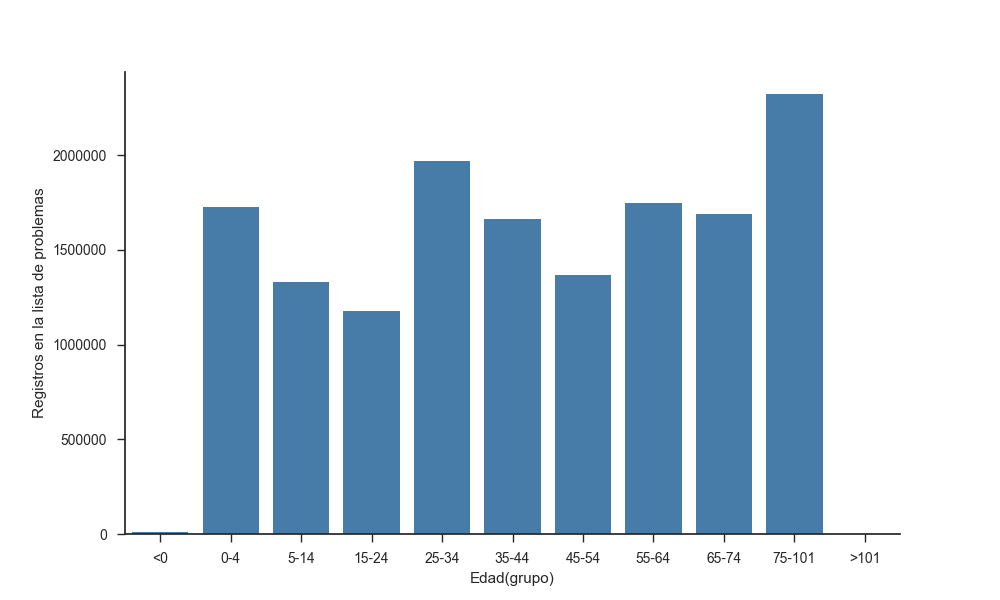
\includegraphics[width=\textwidth]{chart4}
\end{figure}

% Please add the following required packages to your document preamble:
% \usepackage{booktabs}
\begin{table}[htb]
\centering
\caption{Distribución de conceptos por grupo etario }
\label{grupo_etario}
\begin{tabular}{@{}lrr@{}}
\toprule
Grupo Etario & Diferentes Conceptos & Conceptos del grupo \\ \midrule
0-4 & \num{15264} & \num{12532} \\
5-14 & \num{24837} & \num{0} \\
15-24 & \num{29548} & \num{12532} \\
25-34 & \num{35419} & \num{12532} \\
35-44 & \num{33165} & \num{12532} \\
45-54 & \num{32644} & \num{6731} \\
55-64 & \num{35733} & \num{5073} \\
65-74 & \num{35772} & \num{5165} \\
75-101 & \num{37625} & \num{4292} \\ \bottomrule
\end{tabular}
\end{table}

\section{Discusión}
El objetivo de este capítulo era el análisis descriptivo de los datos y de los procesos de limpieza que apliqué para obtener un conjunto de datos consistente con el que realizar los experimentos de graphmining en el siguiente capítulo.

En la primera sección abordé la comprensión de los datos de la lista de problemas. Este análisis me permitió identificar outliers y datos de error al momento de la carga, revisando la distribución desde diferentes dimensiones: tiempo, individuos, conceptos y contextos: 

(a) en el caso del tiempo sólo son válidos los registros con fecha de carga desde el año 1998 hasta el tiempo presente, dado que este ha sido el lapso en el que ha estado activa la HCE; 

(b) desde el punto de vista de los individuos  el 34.1\% tiene sólo un problema, estos registros también se descartan porque carecen de co-ocurrencia con otros problemas; 

(c) en la dimensión de los conceptos, el 20\% de los registros pertenecen a 12 conceptos y sus variantes lexicográficas, estos problemas tendrán poca capacidad predictiva dado que se relacionarán con un número grande de conceptos. El uso de los conceptos presenta una distribución de cola larga, esto es consistente por lo reportado por Fung et. al.\cite{Fung2015AnCT} donde haciendo una comparación del uso de la lista de problemas de ocho instituciones, encontró que el 95\% del uso corresponde a sólo el 22.8\% de términos únicos;

(d) Los contextos analizados fueron el área jerárquica, nivel de asistencia y grupo etario, cada uno de estos contextos tiene sus particularidades.

El HIBA tiene 601 áreas jerárquicas con diferentes niveles de agregación, algunas de esas áreas corresponden a funciones administrativas. El experimento 1 permitió excluir las áreas administrativas y mapear las restantes a  44 servicios de SNOMED CT, facilitando así la interoperabilidad con otros centros médicos. 

El experimento 2 mostró que algunos de los servicios se solapan entre sí, ya que significativamente un clasificador no puede diferenciar cuándo los conceptos pertenecen a un servicio u otro, entre los servicios con F1 score más bajos tengo: servicio de anestesia (0,048), servicio audiológico (0,000), servicio de colposcopia (0,000), servicio de internación domiciliaria (0,131), servicio de patología (0,000) y servicio de psicología (0,000). Estos servicios fueron fusionados con los que más presentaban solapamiento en la matriz de confusión.

Los servicios con mejor F1 score son: servicio de cardiología pediátrica (0,871), servicio de fisioterapia (0,993), servicio de ginecoobstetricia (0,877), servicio de oftalmología adultos (0,938), servicio de psiquiatría (0,827), servicio de psiquiatria pediatrica(0,945) y  servicio de traumatología (0,821). Estos valores muestran que los conceptos diferencian bien estos servicios, y que no deberían ser fusionados aunque uno sea padre del otro como el caso de  servicio de psiquiatría y servicio de psiquiatria pediatrica.

Como resultado de esos experimentos obtuve 29 servicios finales, para evaluar el cubrimiento de los \textit{refsets}, use como referencia los donados por Kaiser Permanente a Snomed CT, en ellos encontré 10 \textit{refsets} de Kaiser Permanente que eran afines a 16 de los 29 servicios finales. Los resultados obtenidos muestran que la mayoría de los servicios tienen una cobertura entre 0,30 y 0,45, los que se ubican con mejor cobertura son pediatría (0,56), cardiología(0,46) y dermatología (0,45); y el de peor cobertura es oncología (0,07), este es el único caso en el que el \textit{refset} creado por el HIBA es de menor tamaño al de referencia, en todos los otros casos el tamaño de los \textit{refsets} del HIBA es superior en tamaño a los de referencia. 

Los niveles de precisión entre los dos conjuntos de datos hace compleja la tarea de comparación, cuando cuento los conceptos que se encuentran en el \textit{refset} de referencia, no sólo debo de tener en cuenta los mapeos directos o las relaciones is\_a exactas, porque pierdo a los conceptos que tienen mayor precisión. Por lo tanto, contrasté estos resultados con la cobertura calculada con diferentes distancias semánticas, encontrando que hay una significativa mejora en los valores de cubrimiento, incluso con distancia \textless= 2 la mayoría de los servicios alcanzan más de un 90\% de cubrimiento de conceptos del Kaiser.

Un trabajo similar reportado por Nova Scotia\cite{nova}, en el que desarrollan sus propios \textit{refsets} de especialidades, obtiene coberturas inferiores a las reportadas en esta tesis, incluso sin el cálculo de distancias semánticas (ver tabla \ref{coverage_scotia}). 

\begin{table}
 \caption{Comparación de la cobertura de las especialidades del HIBA vs Nova Scotia }
  \label{coverage_scotia}
  \resizebox{\textwidth}{!}{%
  \begin{tabular}{lcccccc} \hline
 \small
& \multicolumn{3} {c}{ Nova Scotia} & \multicolumn{3} {c}{HIBA} \\ \hline
Servicio& \# Refset & \# Kaiser & Cobertura &\# Refset & \# Kaiser  & Cobertura  \\ \hline
Cardiología&886&653 &0,18&9182&880  &0,46 \\
Dermatoloía&638&691    &0,16&11622&2757     &0,45 \\
Hematología*&714&330   &0,13&721&4086    &0,17\\
Enfermedades infecciosas&2,202&1101   &0,08&-&-&  \\
Oftamología&1,327&413&    0,34&4188&3285     &0.41\\
Cirugía ortopédica&1,306&167&   0,10&22555&1089    &0,25\\
Otoloaringología&1,344&641    &0,29&-&-&  \\
Pediatría&3,699&2181    &0,34&17325&3793     &0,56\\
Medicina respiratoria&114&511   &0,08&-&-&\\\hline

\end{tabular}
 %
}
\end{table}

En el nivel de asistencia hay desbalanceo entre los grupos. Los grupos más grandes son el nivel de asistencia ambulatorio (6304 conceptos), las internaciones que se fusionaron en una sola (3002), y la guardia (2269). Aunque el nivel de asistencia de Triage sea el tercero en cantidad de registros, el número de conceptos en su grupo es muy pequeño, lo que indica la baja diversidad de conceptos seleccionados en este nivel de asistencia. 

Los grupos etarios que más registran problemas son entre los 0-4 años, 25 y 34 años y mayores de 75 años, los registros con edades menores a 0 o mayores a 101 fueron descartadas por interpretarse como errores del sistema o casos de prueba. Utilizando los algoritmos de agrupación se fusionaron los grupos etarios entre los 0 y 44 años. Según estos algoritmos, los problemas que existen en estos grupos no tienen diferencias significativas. Al mismo tiempo, descarté el grupo etario entre 5 y 14 años, ya que los problemas no se agruparon en un grupo consistente.

\section{Conclusión}
En este capítulo he presentado las decisiones en la extracción, transformación y limpieza de la lista de problemas, para definir el conjunto de datos que será utilizado en los experimentos de graphmining. 

La transformación más compleja fue la de la definición del contexto de los 29 servicios de atención a partir de las 901 áreas jerárquicas. Si bien agrupar los conceptos por contexto es necesario para facilitar el uso significativo de la SNOMED CT, son escasos los ejemplos sobre metodologías o \textit{refsets} públicos que puedan ser usados como referencia.

En este capítulo usé técnicas de agrupamiento y aprendizaje supervisado para definir qué servicios, niveles asistenciales y grupos etarios pueden ser diferenciables de los demás a partir de sus conceptos. En el caso de los servicios, Una vez fueron definidos evalué su cubrimiento con respecto a los \textit{refsets} de referencia de kaiser permanente, aunque en la mayoría de los casos da un cubrimiento exacto superior al 40\%, si se utilizan las distancias semánticas estos cubrimientos se incrementan significativamente.

Con respecto a las distancias semánticas, este trabajo no tiene en cuenta el nivel de granularidad de los conceptos que se están comparando, por lo tanto un par de conceptos que estén muy arriba en la jerarquía y sean muy generales tienen igual distancia que dos conceptos que estén muy abajo y sean muy específicos. Sin embargo, en la práctica entre más precisos sean los conceptos que tienen similitud, se puede confiar más en que realmente tienen un significado similar.

 
\chapter{Capítulo: Resultados del análisis de redes}
%%%% Resultados Parte 2
\section{Introducción}
En los capítulos anteriores realicé una revisión del estado del arte sobre el \textit{graph mining} aplicado en el área de la salud, con las definiciones en las cuales se enmarca esta tesis. Además, describí el proceso para obtener el conjunto de datos de la lista de problemas y los contextos de servicios de atención de salud, nivel asistencial y grupo etario. 

Este capítulo contiene la construcción de dos grafos. El primero con las relaciones a Snomed CT, y el segunda sin las relaciones. Ya que es de interés analizar si las conexiones de Snomed CT mejoran la capacidad de formar comunidades y su capacidad predictiva.

El análisis se compone de la aplicación de las definiciones de los grafos descriptas en los capítulos anteriores, evaluando si los grafos formados siguen patrones de redes de gran escala. Además del análisis sobre los agrupamientos encontrados luego de aplicar los algoritmos \textit{label propagation}, \textit{leading vector} y \textit{multilevel}. 

Finalmente, se evaluará la capacidad predictiva de los conceptos que están en el mismo grupo dada una lista de problema de un paciente. Esta evaluación se realizará usando los {\acrshort{refset}} de los contextos como vocabularios controlados.

\section{Definición del grafo}
Sea el grafo de la figura\ref{fig:ModeloGrafo} G=(V,E), donde V denota a los vértices, equivalente a nodos: conceptos de snomed CT y pacientes, y E denota las aristas, equivalente a relaciones: \textit{tiene un problema}, o conexiones jerárquicas $|\textit{ES\_UN}|$  (Hallazgo Clínico, Procedimientos, Eventos, Situación con contexto explícito). Las propiedades de nivel asistencial, servicio de atención  y grupo etario pertenecen a la arista {tiene un problema}, ya que un mismo paciente puede acudir al hospital por el mismo problema en diferentes contextos.  Si un mismo paciente acude varias veces con el mismo contexto, esa información se registra en la propiedad frecuencia. A la derecha de la figura\ref{fig:ModeloGrafo} se observa una instancia del modelo, donde el paciente identificado con el id \textbf{12345} tiene:
\begin{itemize}
\item el problema \textbf{Varicela}; 
\item el contexto de este problema es el nivel asistencia de la \textbf{Guardia}, el servicio de atención de salud es \textbf{Pediatría}, y el grupo etario es entre \textbf{5 y 14 años}; 
\item el paciente acudió \textbf{dos} veces al hospital con el mismo contexto y el mismo problema.
\item Según Snomed CT, la \textbf{varicela} es una \textbf{enfermedad viral caracterizada por exantema} y es una \textbf{infección por virus varicela zoster}.
\end{itemize}


Los \num{88869} conceptos distintos de la lista de problemas están relacionados jerárquicamente con \num{11946} de Snomed CT, de tal manera que al usar todos los conceptos de las jerarquías, el número de vértices y aristas de la red son $|V|=$\num{19354} y $|E|=$\num{1173234} respectivamente. 

Se realiza el mismo análisis sobre el subgrafo generado sólo con las relaciones \textit{tiene un problema} y los nodos que comparten esta relación. El número de vértices y aristas de este subgrafo son $|V|=$\num{11946} y $|E|=$\num{937107} respectivamente.

Para diferenciar las dos redes, la primera la nombro como \textbf{\acrfull{RP-SCT}} y la segunda la nombro como \textbf{{\acrfull{RP}}}

\begin{figure}[ht]
\caption{Modelo de datos de grafos de la lista de problemas}
\label{fig:ModeloGrafo}
\centering
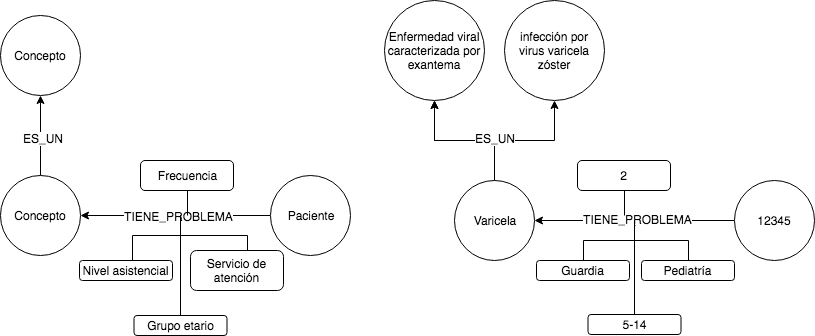
\includegraphics[width=\textwidth]{Modelo_de_datos_Problemas}
\end{figure}

\section{Patrones de la red de la lista de problemas}
\subsection{Red libre de escala}
En esta sección evalúo si la redes comparte patrones con redes de gran escala, realizo (1) ajuste a una distribución de ley de potencias usando los grados de cada nodo y (2) comparación con las distribuciones exponencial y logarítmica.

En el caso de la \textbf{\acrshort{RP-SCT}} la función \acrshort{cdf} es:
\begin{equation}
F(X\geq 51) \propto x^{-1.82 +1}
\end{equation}

El p-value$(0.3188>0.05)$ no me permite rechazar la hipótesis nula.

En la tabla \ref{distribucionRPSCT} están los resultados de las comparaciones realizadas entre ley de potencias con otras distribuciones: la distribución exponencial fue usada para confirmar que los datos tienen una cola pesada, y la distribución lognormal tiene un mejor ajuste que la ley de potencias, como se muestra también en la figura \ref{fig:ajusteDistribuciones}.

% Please add the following required packages to your document preamble:
% \usepackage{booktabs}
\begin{table}[htb]
\centering
\caption{Comparación de la ley de potencias con otras distribuciones de la \textbf{\acrshort{RP-SCT}}}
\label{distribucionRPSCT}
\begin{threeparttable}
\begin{tabular}{@{}lr@{}}
\toprule
Distribución & Resultado    \\ \midrule
Exponencial  & 10.64\tnote{*}  \\
Lognormal    & -1.5 \\ \bottomrule
\end{tabular}
\begin{tablenotes}
    \item[*] p-value$<$\num{0.05}.
  \end{tablenotes}
\end{threeparttable}
\end{table}

\begin{figure}[ht]
\caption{Gráfico log-log, comparación de ajuste de distribuciones de la red semántica de problemas}
\label{fig:ajusteDistribuciones}
\centering
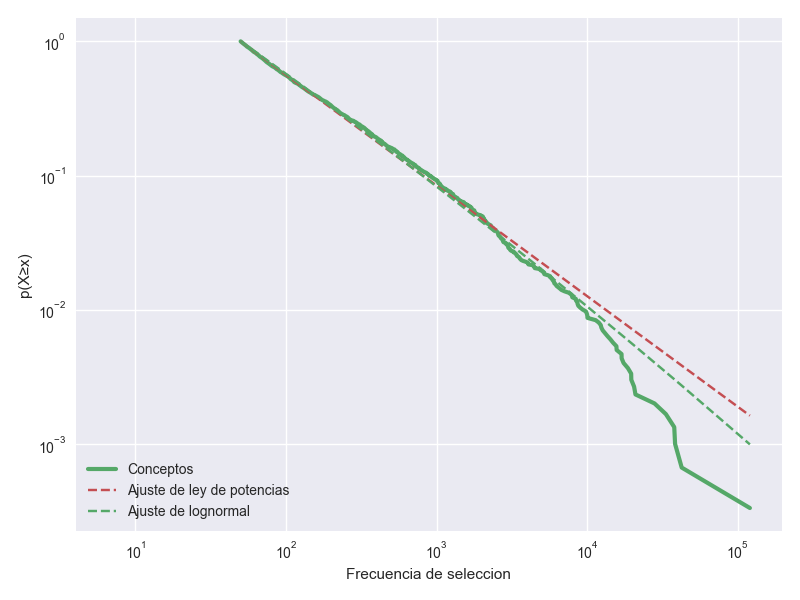
\includegraphics[width=0.6\textwidth]{chart6}
\end{figure}

En el caso de la \textbf{\acrshort{RP}} la función \acrshort{cdf}  es:
\begin{equation}
F(X\geq 279) \propto x^{-1.86 +1}
\end{equation}

Con el p-value$(0.03<0.05)$ se acepta la hipótesis nula los datos se distribuyen según la ley de potencias. La figura \ref{fig:ajusteDistribucionesRP} y la tabla \ref{distribucionRP} muestra también que esta distribución tiene mejor ajuste.

\begin{table}[htb]
\centering
\caption{Comparación de la ley de potencias con otras distribuciones de la \textbf{\acrshort{RP}}}
\label{distribucionRP}
\begin{threeparttable}
\begin{tabular}{@{}lr@{}}
\toprule
Distribución & Resultado    \\ \midrule
Exponencial  & 4.64\tnote{*}  \\
Lognormal    & -2.41 \\ \bottomrule
\end{tabular}
\begin{tablenotes}
    \item[*] p-value$<$\num{0.05}.
  \end{tablenotes}
\end{threeparttable}
\end{table}

\begin{figure}[ht]
\caption{Gráfico log-log, comparación de ajuste de distribuciones de la \textbf{\acrshort{RP}}}
\label{fig:ajusteDistribucionesRP}
\centering
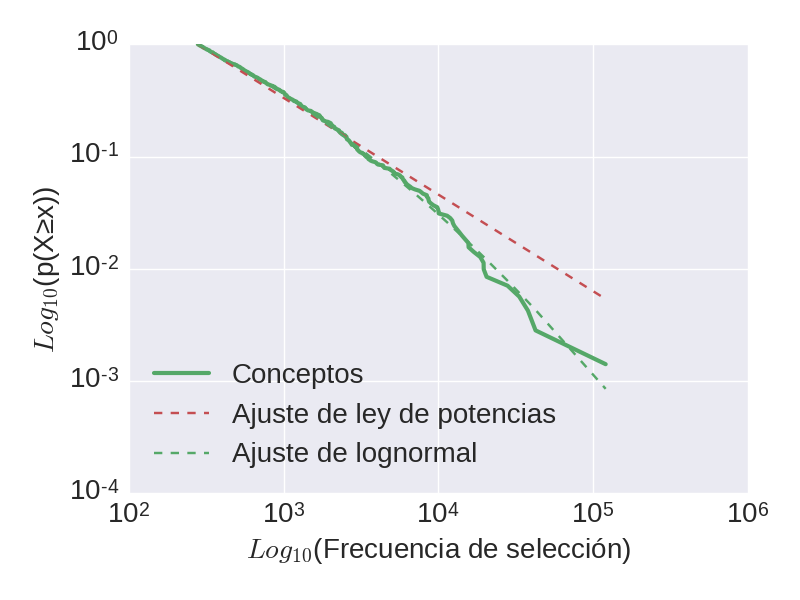
\includegraphics[width=0.6\textwidth]{chart7}
\end{figure}


\subsection{Estructuras de comunidad}
Existen diferentes métricas para evaluar cuantitativamente los efectos de comunidad en un grafo, las usadas  a continuación siguen el trabajo de Boccaletti \textit{et. al}\cite{BOCCALETTI2006} y los detalles se encuentran en el marco teórico. (Ver sección \ref{par:efecto-comunidades})

\begin{table}[htb]
\centering
\caption{Métricas de efectos de comunidad en redes}
\label{community-graphs}
\resizebox{\textwidth}{!}{%
\begin{tabular}{@{}lrr@{}}
\toprule
Métrica                                                  & Valor en la \acrshort{RP-SCT}  & Valor en la \acrshort{RP}            \\ \midrule
Coeficiente de agrupamiento - transitividad                & \num{0.19} & \num{0.21} \\
Coeficiente de agrupamiento - transitividad local promedio & \num{0.41}  & \num{0.80}\\
Coeficiente de agrupamiento promedio                        & \num{0.34}  & \num{0.78}      \\
Longitud media del camino mínimo entre nodos             & \num{2.80}  & \num{2.17}  \\
Promedio de grados                                       & \num{60.62}  & \num{78.4}      \\ \bottomrule
\end{tabular}%
}
\end{table}

Los valores de coeficiente de agrupamiento cercanos a 1 indican alto grado de agrupamiento, como se puede ver en la tabla \ref{community-graphs} la \textbf{\acrshort{RP}} tiene mejores coeficientes que la \textbf{\acrshort{RP-SCT}}. 

\section{Agrupamiento}

Apliqué los algoritmos de agrupamiento: \textit{label propagation}, \textit{leading vector} y \textit{multilevel} a el grafo de la \textbf{\acrshort{RP}} y a sub-grafos de la  \textbf{\acrshort{RP-SCT}}, conformados por relaciones que tengan un mínimo de frecuencia en pacientes (\num{5}, \num{10}, \num{100}, \num{1000} y \num{10000}). Esto con el propósito de evaluar la estabilidad de los agrupamientos aunque el grafo pierda nodos.

La tabla \ref{res_agru} contiene los resultados de la modularidad y la cantidad de grupos encontrados al aplicar los algoritmos de agrupamiento. Se puede observar que en el caso del grafo de la \textbf{\acrshort{RP}}  se generan similares número de grupos aunque la modularidad varía en los algoritmos. La modularidad más alta es el del algoritmo \textit{multilevel} y el más bajo es el de \textit{label propagation}.

En el caso de los sub-grafos \textbf{\acrshort{RP-SCT}}, el número de grados varía entre algoritmos: \textit{multilevel} es también el que mejores modularidades obtiene y mientras que \textit{leading vector} va desmejorando en su modularidad a medida que crece el grafo, \textit{label propagation} mejora. 

% Please add the following required packages to your document preamble:
% \usepackage{booktabs}
% \usepackage{multirow}
% \usepackage{graphicx}
\begin{table}[htb]
\centering
\caption{Resultados de agrupamiento de grafos de problemas}
\label{res_agru}
\resizebox{\textwidth}{!}{%
\begin{tabular}{@{}lrrrrrr@{}}
\toprule
\multirow{3}{*}{Grafo}                                                                                          & \multicolumn{6}{l}{Algoritmos de agrupamiento}                                                                                                                                             \\ \cmidrule(l){2-7} 
                                                                                                                & \multicolumn{2}{l}{Leading Vector}                           & \multicolumn{2}{l}{Multilevel}                               & \multicolumn{2}{l}{Label Propagation}                        \\ \cmidrule(l){2-7} 
                                                                                                                & \multicolumn{1}{l}{Modularidad} & \multicolumn{1}{l}{Grupos} & \multicolumn{1}{l}{Modularidad} & \multicolumn{1}{l}{Grupos} & \multicolumn{1}{l}{Modularidad} & \multicolumn{1}{l}{Grupos} \\ \cmidrule(r){1-7}
Red de Problemas(\acrshort{RP})                                                                                                & 0.36                            & 22                         & 0.43                            & 23                         & 0.08                            & 22                         \\
\begin{tabular}[c]{@{}l@{}}Red Semántica de Problemas \\ (Relaciones en al menos 10000 individuos)\\(\acrshort{RP-SCT}-10.000)\end{tabular} & 0.50                            & 14                         & 0.59                            & 27                         & 0.27                            & 87                         \\
\begin{tabular}[c]{@{}l@{}}Red Semántica de Problemas \\ (Relaciones en al menos 1000 individuos)\\(\acrshort{RP-SCT}-1.000)\end{tabular}  & 0.50                            & 14                         & 0.59                            & 27                         & 0.27                            & 88                         \\
\begin{tabular}[c]{@{}l@{}}Red Semántica de Problemas \\ (Relaciones en al menos 100 individuos)\\(\acrshort{RP-SCT}-100) \end{tabular}   & 0.50                            & 14                         & 0.59                            & 24                         & 0.29                            & 92                         \\
\begin{tabular}[c]{@{}l@{}}Red Semántica de Problemas \\ (Relaciones en al menos 10 individuos)\\(\acrshort{RP-SCT}-10) \end{tabular}    & 0.29                            & 11                         & 0.61                            & 24                         & 0.37                            & 91                         \\
\begin{tabular}[c]{@{}l@{}}Red Semántica de Problemas \\ (Relaciones en al menos 5 individuos)\\(\acrshort{RP-SCT}-5)\end{tabular}     & 0.32                            & 12                         & 0.62                            & 25                         & 0.46                            & 88                         \\ \bottomrule
\end{tabular}%
}
\end{table}

Estos seis grafos con sus 3 algoritmos representan grupos fuertes y débiles, a continuación presento los grupos de problemas que son consistentes en todos los agrupamientos. Además calculo la longitud media del camino mínimo entre los nodos del agrupamiento, esta información permite detectar grupos con conceptos con diferentes significados semánticos y valores atípicos.

\subsection{Agrupamientos de Red de Problemas }
Combinando los resultados de los agrupamientos hay \num{11132} posibles combinaciones, encontré 53 grupos de problemas que comparten las mismas agrupaciones. Según la tabla, \ref{gruposRP} la mayoría (19) de los grupos encontrados tienen 2 nodos, los grupos que tiene más nodos tienen en promedio una mediana de grados por nodo más grande, es decir que son nodos altamente conectados.

Al analizar las distancias semánticas entre los conceptos que comparten el mismo grupo, puedo observar según la figura \ref{fig:bpDistanciasSemanticasRP} que la mayoría de las medianas de las distancias se ubican cercanas a 10. Los grupos con las mayores dispersiones son el cluster\_1, cluster\_6, cluster\_10, cluster\_16, cluster\_22, cluster\_27, cluster\_30, cluster\_34 y cluster\_36. 

En la tabla \ref{top10_rp} se encuentra los conceptos con más altas medidas de  centralidad (grado, cercanía e intermediación). En esta tabla se encuentran sólo los casos que contienen las mayores dispersiones según la distancia semántica. Se puede observar que coinciden los conceptos con los más altas métricas según el grado y la cercanía, y que difiere en el caso de la intermediación. En la métrica de intermediación se encuentran conceptos que sin tener muchas conexiones son mucho más importantes para la conexión de otros dos vértices del grafo.

Por ejemplo, según lo anterior en el caso del cluster\_6 (que se puede interpretar como de enfermedades generales), los problemas con mayor grado (los más populares) son: FIEBRE (SCTID: 386661006) y TOS (SCTID: 49727002), pero el problema con mayor intermediación es RESFRIÓ COMÚN (SCTID: 82272006). Es decir, que este último conecta más otros pares de problemas que la Fiebre y la Tos. Otros ejemplos se pueden encontrar en el cluster\_10, donde el problema con mayor grado y cercanía es MALESTAR GENERAL (SCTID: 367391008), y el de mayor intermediación es INMUNODEFICIENCIA COMBINADA SEVERA (SCTID: 31323000); y en el grupo de embarazo (cluster\_16) donde los problemas con mayor grado son PACIENTE ACTUALMENTE EMBARAZADA (SCTID: 77386006) , ANSIEDAD (SCTID: 48694002) y MAREO (SCTID: 404640003), pero los de mayor intermediación son AMENAZA DE TRABAJO DE PARTO PREMATURO (SCTID: 6383007), INTOXICACIÓN POR FÁRMACO Y/O SUSTANCIA MEDICINAL (SCTID: 7895008) y SANGRADO VAGINAL (SCTID: 268471004).

\subsubsection{Valores atípicos}
Según el boxplot generado con las distancias semánticas en la figura \ref{fig:bpDistanciasSemanticasRP}, se presentan valores atípicos en los siguientes grupos:
\begin{itemize}
\item cluster\_6: Este es un agrupamiento de enfermedades generales donde los problemas que tiene mayor distancia semántica en promedio con el resto del mismo grupo es: CIRUGÍA DE CATARATAS(PROCEDIMIENTO) (SCTID: 110473004), ATAQUE DE PÁNICO(HALLAZGO) (SCTID: 225624000), AMIGDALECTOMÍA(PROCEDIMIENTO) (SCTID: 173422009)
\item cluster\_10: Este es un agrupamiento de administración de medicamentos y procedimientos invasivos, los problemas con mayores distancias son: ADMINISTRACIÓN DE ANTICOAGULANTE(PROCEDIMIENTO) (SCTID: 71788004), TRATAMIENTO CON ANTIBIÓTICOS INTRAVENOSOS(PROCEDIMIENTO) (SCTID: 281790008), INYECCIÓN DE GAMMAGLOBULINA (PROCEDIMIENTO) (SCTID: 180191005), CAMBIO DEL TUBO DE TRAQUEOSTOMÍA (PROCEDIMIENTO) (SCTID: 2267008). Estas distancias se explican porque la mayoría de los conceptos de este grupo están en la jerarquía de Hallazgos.
\item cluster\_27: En este agrupamiento de enfermedades relacionadas con la edad avanzada, los problemas que tienen mayor distancia son: CONFUSIÓN AGUDA(HALLAZGO) (SCTID: 130987000), PACIENTE EN CAMA (HALLAZGO) (SCTID: 160685001).
\item cluster\_36: En este agrupamiento de enfermedades cardiopulmonares, las mayores distancias se encuentran en los siguientes conceptos: BIOPSIA ENDOMIOCÁRDICA (PROCEDIMIENTO) (SCTID: 387829002), ALOTRASPLANTE ORTOTÓPICO DE CORAZÓN (PROCEDIMIENTO) (SCTID: 232974001) y TUMOR DE KLATSKIN (TRASTORNO) (SCTID: 253017000), esta última considerada como una enfermedad huérfana\footnote{www.orpha.net/consor/cgi-bin/OC\_Exp.php?lng=ES\&Expert=99978}.
\end{itemize}

Los valores atípicos en las cotas inferiores, donde las distancias semánticas son cercanas a 1,  se debe a relaciones entre conceptos ancestros y sus descendientes. Por ejemplo: en el cluster\_42: EPISTAXIS ANTERIOR (SCTID: 232354002) es descendiente de EPISTAXIS (SCTID: 249366005), y ambos conceptos están en el mismo grupo.

% Please add the following required packages to your document preamble:
% \usepackage{booktabs}
\begin{table}[htb]
\centering
\caption{Grupos que comparten las mismas agrupaciones en la red de problemas}
\label{gruposRP}
\begin{tabular}{@{}rrr@{}}
\toprule
Número de Nodos & Grupos Encontrados & Mediana de grados por nodo \\ \midrule
2               & 19                 & 1949                       \\
3               & 9                  & 1832                       \\
4               & 5                  & 1833                       \\
5               & 1                  & 1818                       \\
6               & 5                  & 3287                       \\
7               & 1                  & 1590                       \\
8               & 2                  & 5192                       \\
10              & 2                  & 2222                       \\
13              & 1                  & 802                        \\
16              & 1                  & 990                        \\
22              & 1                  & 2198                       \\
25              & 1                  & 3008                       \\
34              & 1                  & 4210                       \\
45              & 1                  & 864                        \\
59              & 1                  & 3700                       \\
77              & 1                  & 1228                       \\
84              & 1                  & 3234                       \\ \bottomrule
\end{tabular}
\end{table}

\begin{figure}[ht]
\caption{Distancias semánticas entre conceptos de los agrupamientos de la \acrshort{RP}}
\label{fig:bpDistanciasSemanticasRP}
\centering
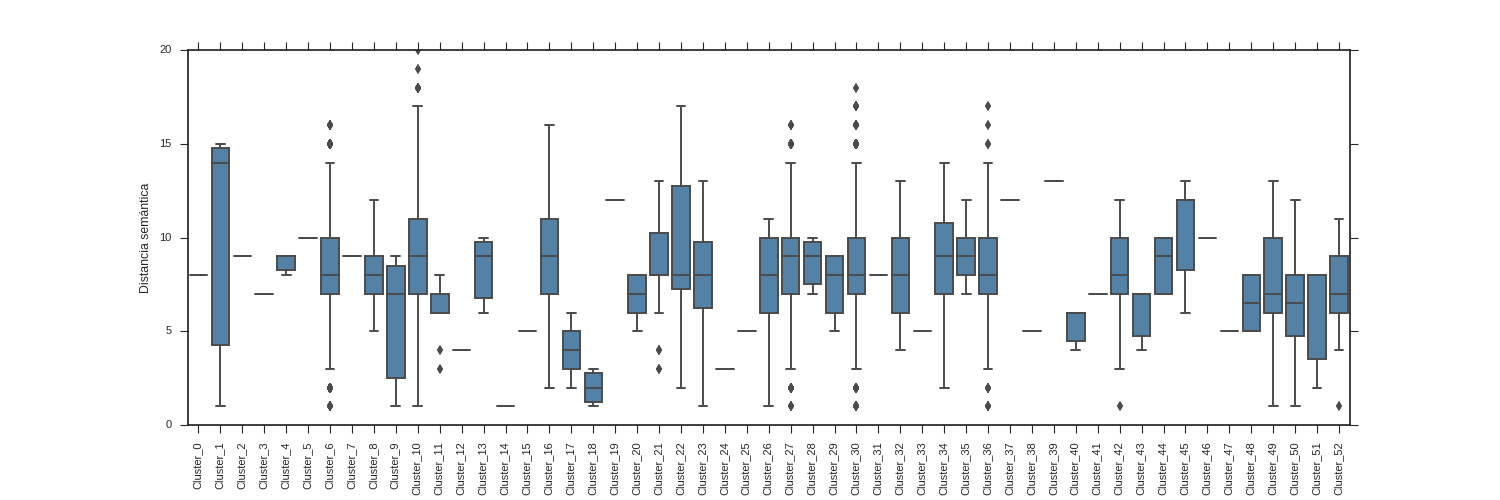
\includegraphics[width=\textwidth]{bpDistanciasSemanticasRP}
\end{figure}

\subsection{Agrupamientos de Red Semántica de Problemas}
Combinando los resultados de los agrupamientos utilizando cualquier algoritmo de clasificación, hay \num{2,39e26} posibles combinaciones. Encontré 68 grupos de problemas que comparten las mismas agrupaciones. Según la tabla \ref{gruposRSP} La mayoría (44) de los grupos encontrados tienen 2 nodos.

Al analizar las distancias semánticas entre los conceptos que comparten el mismo grupo, puedo observar según la figura \ref{fig:bpDistanciasSemanticasRSP} que las medianas de las distancias tienen un mínimo de 1 y máximo de 10. A diferencia de la de \acrshort{RP},  en la \acrshort{RP-SCT}, las medianas de la distancia semántica no son constantes. 

En la tabla \ref{top10_rsp} se encuentra los conceptos con más altas medidas de  centralidad (grado, cercanía e intermediación). Estos grupos son más pequeños que en la \acrshort{RP}, pero sobresalen los grupos con distancias semánticas grandes cuyos conceptos pareciera que no están muy relacionados, por ejemplo, el cluster\_0: INCISIÓN DE LA TRÁQUEA (SCTID: 48387007), AMIGDALECTOMÍA(SCTID: 173422009) y CIRUGÍA DE CATARATAS (SCTID: 110473004), el cluster\_2: FÍSTULA TRAQUEOESOFÁGICA (SCTID: 95435007) y ÚTERO UNICORNE (SCTID: 1372004), el cluster\_6: HIPERCORTISOLISMO (SCTID: 47270006) y TUMOR DE KLATSKIN (SCTID: 253017000). Sin embargo, al hacer una búsqueda rápida se pueden encontrar evidencias de las relaciones de estas enfermedades en artículos de divulgación científica, como se muestra en la tabla \ref{evidencia_grupos_2}.

Observando las diferencias de los resultados entre las dos redes, entre los grupos que estaban en la \acrshort{RP} y desaparecen en la \acrshort{RP-SCT},  se encontró evidencia de casos que son distantes semánticamente y que se encuentran en el mismo grupo en \acrshort{RP} , Ejemplos:
\begin{itemize}
\item Distancia 10, Defecto ventilatorio (SCTID: 11483009) y Problema nasal  (SCTID: 301199001).
\item Distancia 13, Alergia (SCTID: 106190000)  y Dermatitis atópica (SCTID: 24079001).
\item Distancia 4, Náuseas y vómitos (SCTID:16932000)  y Hallazgo relacionado con el vómito (SCTID:300359004)
\end{itemize}

Por otra parte, hay grupos que se generaron en \acrshort{RP-SCT} y no aparecen en  \acrshort{RP}.  Los conceptos tienen distancias semánticas pequeñas,  ejemplos:
\begin{itemize}
\item Distancia 2, Hipertiroidismo (SCTID:  34486009) y trastorno del cuello (SCTID: 118939000).  Hipertiroidismo es un hijo de trastorno del cuello
\item Distancia 2, Mucositis ulcerosa de cuello uterino (SCTID: 428193004) y Rinitis (SCTID:  70076002). Ambos son hijos de enfermedad inflamatoria de las membranas mucosas.
\item Distancia 2, Enfermedad inflamatoria pélvica aguda  (SCTID:237037006) y Absceso agudo de la mama  (SCTID:16698000). Ambos son hijos de trastorno inflamatorio agudo.
\end{itemize}


\subsubsection{Valores atípicos}
Según el boxplot generado con las distancias semánticas en la figura \ref{fig:bpDistanciasSemanticasRSP}, se presentan valores atípicos sólo en el grupo cluster\_56 formado por: PROCTORRAGIA (SCTID: 12063002), INDIGESTIÓN (SCTID: 162031009), DISFAGIA (SCTID: 40739000), VEJIGA: INCONTINENTE (SCTID: 165232002), CÁLCULO RENAL (SCTID: 95570007), HEMORRAGIA DIGESTIVA BAJA (SCTID: 87763006), SÍNDROME DE ICTERICIA COLESTÍSICA (SCTID: 44018007) y PIELONEFRITIS (SCTID: 45816000). Los problemas con mayores distancias son VEJIGA: INCONTINENTE (SCTID: 165232002) y SÍNDROME DE ICTERICIA COLESTÍSICA (SCTID: 44018007).


% Please add the following required packages to your document preamble:
% \usepackage{booktabs}
\begin{table}[htb]
\centering
\caption{Grupos que comparten las mismas agrupaciones en la red semántica de problemas}
\label{gruposRSP}
\begin{tabular}{@{}rrr@{}}
\toprule
Número de Nodos & Grupos Encontrados & Mediana de grados por nodo \\ \midrule
2	& 44	&2041 \\
3	&12 &	2144\\
4	&3&	1843\\
5	&4&	1826\\
6	&2&	1226\\
8	&2&	3501\\
9	&1&	1172                   \\ \bottomrule
\end{tabular}
\end{table}

\begin{figure}[ht]
\caption{Distancias semánticas entre conceptos de los agrupamientos de la \acrshort{RP-SCT}}
\label{fig:bpDistanciasSemanticasRSP}
\centering
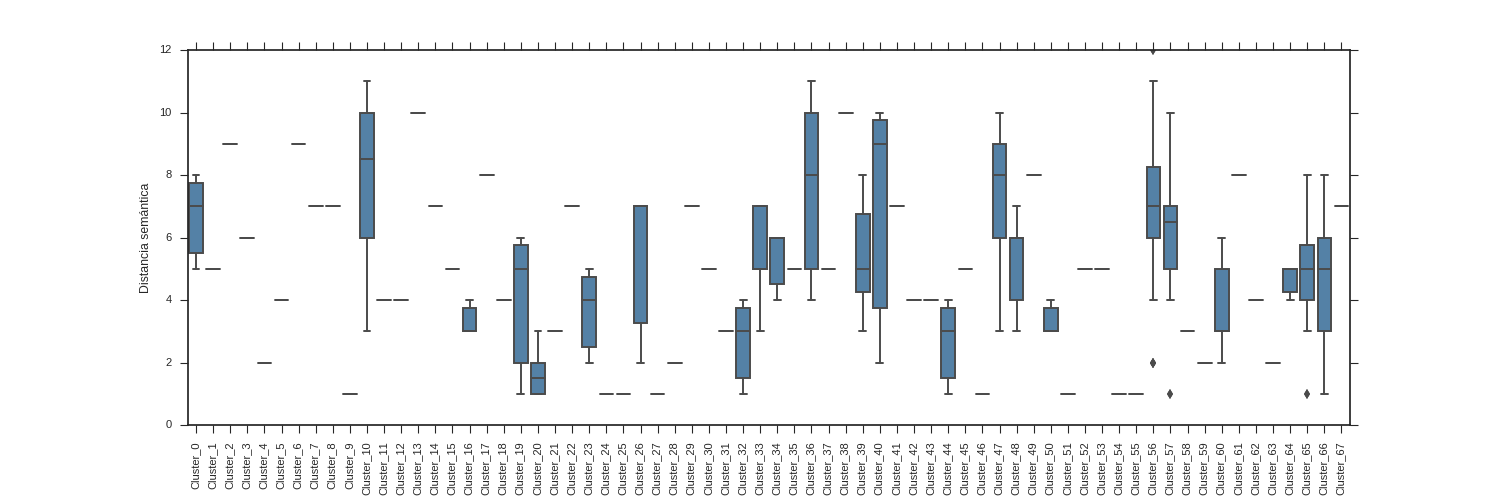
\includegraphics[width=\textwidth]{bpDistanciasSemanticasRSP}
\end{figure}

\subsubsection{Agrupamientos \textit{Label Propagation}}
Combinando los resultados de aplicar sólo el algoritmo \textit{label propagation} en la \acrshort{RP-SCT} con diferentes cantidades mínimas de individuos que tengan el problema (RP-SCT-10.000,RP-SCT-1.000, RP-SCT-100,RP-SCT-10 y RP-SCT-5) , hay \num{5.64e9} posibles combinaciones (Ver tabla \ref{res_agru}) .  De estas combinaciones hay 232 grupos comunes a todos los resultados de agrupamiento. 

Los 232 grupos tienen las siguientes características: más del 50\% de los grupos tienen menos de 50 nodos, estos grupos son muy cohesivos, ya que tienen distancias en promedio de dos saltos entre vértices y con una baja cantidad total de distancias atípicas a los otros vértices del grupo (10 en total en 144 grupos). Los grupos más grandes tienen también la mayor cantidad de vértices con valores de distancias atípicas.

% Please add the following required packages to your document preamble:
% \usepackage{booktabs}
% \usepackage{graphicx}
\begin{table}[htb]
\centering
\caption{Agrupamientos recurrentes en la red \acrshort{RP-SCT}con el algoritmo \textit{Label propagation}}
\label{clus_lp}
\resizebox{\textwidth}{!}{%
\begin{tabular}{@{}lrrrrrr@{}}
\toprule
\multirow{2}{*}{Número de nodos}                                                                                          & \multicolumn{6}{c}{Estadísticos de distancia entre nodos}                                                                                                                                             \\ \cmidrule(l){2-7} 
&  \multicolumn{1}{l}{\begin{tabular}[c]{@{}l@{}}Número de \\ agrupamientos\end{tabular}} & \multicolumn{1}{l}{\begin{tabular}[c]{@{}l@{}}Promedio\end{tabular}} & \multicolumn{1}{l}{\begin{tabular}[c]{@{}l@{}}Desviación estándar\end{tabular}} & \multicolumn{1}{l}{\begin{tabular}[c]{@{}l@{}} Máximo\end{tabular}}  & \multicolumn{1}{l}{\begin{tabular}[c]{@{}l@{}}Mínimo\end{tabular}} & \multicolumn{1}{l}{\begin{tabular}[c]{@{}l@{}} Distancias con \\valores atípicos\end{tabular}} \\ \midrule
Menores de 50 nodos & 144 & 2 & 1,7 & 10 & 1 & 10 \\
Entre 50 y 100 nodos & 25 & 2 & 0,8 & 5 & 2 & 34 \\
Entre 100 y 200 nodos & 13 & 3 & 1,4 & 8 & 2 & 0 \\
Entre 200 y 500 nodos & 20 & 3 & 1,1 & 7 & 2 & 56 \\
Entre 500 y 1000 nodos & 10 & 4 & 1,4 & 7 & 3 & 106 \\ 
Mayor de 1000 nodos & 20 & 6 & 1,4 & 9 & 4 & 6600 \\\bottomrule
\end{tabular}%
}
\end{table}

\subsubsection{Agrupamientos \textit{Leading vector}}
Combinando los resultados de aplicar el algoritmo \textit{leading vector} en la \acrshort{RP-SCT} con diferentes cantidades mínimas de individuos que tengan el problema (RP-SCT-10.000,RP-SCT-1.000, RP-SCT-100,RP-SCT-10 y RP-SCT-5) , hay \num{3.62e5}  posibles combinaciones (Ver tabla \ref{res_agru}) .  De estas combinaciones hay 38 grupos comunes a todos los resultados de agrupamiento. 

Según la tabla \ref{clus_lv} el 50\% de los agrupamientos tienen más de 1000 nodos. Los grupos hasta 1000 nodos  son bastante cohesivos, con distancias promedios cercanas a 3 y sin distancias atípicas a los otros vértices del grupo. 

\begin{table}[htb]
\centering
\caption{Agrupamientos recurrentes en la red \acrshort{RP-SCT} con el algoritmo \textit{Leading vector}}
\label{clus_lv}
\resizebox{\textwidth}{!}{%
\begin{tabular}{@{}lrrrrrr@{}}
\toprule
\multirow{2}{*}{Número de nodos}                                                                                          & \multicolumn{6}{c}{Estadísticos de distancia entre nodos}                                                                                                                                             \\ \cmidrule(l){2-7} 
&  \multicolumn{1}{l}{\begin{tabular}[c]{@{}l@{}}Número de \\ agrupamientos\end{tabular}} & \multicolumn{1}{l}{\begin{tabular}[c]{@{}l@{}}Promedio\end{tabular}} & \multicolumn{1}{l}{\begin{tabular}[c]{@{}l@{}}Desviación estándar\end{tabular}} & \multicolumn{1}{l}{\begin{tabular}[c]{@{}l@{}} Máximo\end{tabular}}  & \multicolumn{1}{l}{\begin{tabular}[c]{@{}l@{}}Mínimo\end{tabular}} & \multicolumn{1}{l}{\begin{tabular}[c]{@{}l@{}} Distancias con \\valores atípicos\end{tabular}} \\ \midrule
Menores de 50 nodos & 15 & 3,4 & 2,8 & 9 & 1 & 0 \\
Entre 50 y 100 nodos & 3 & 3 & 1,7 & 5 & 2 & 0 \\
Entre 100 y 200 nodos & 1 & 3 & - & 3 & 3 & 0 \\
Entre 500 y 1000 nodos & 2 & 5,5 & 0,7 & 6 & 5 & 0 \\
Mayor de 1000 nodos & 19 & 7 & 1,2 & 9 & 5 & 50712 
\\\bottomrule
\end{tabular}%
}
\end{table}

\subsubsection{Agrupamientos \textit{Multilevel}}
Combinando los resultados de aplicar el algoritmo \textit{multilevel} en la \acrshort{RP-SCT} con diferentes cantidades mínimas de individuos que tengan el problema (RP-SCT-10.000,RP-SCT-1.000, RP-SCT-100,RP-SCT-10 y RP-SCT-5) , hay \num{1.05e7}  posibles combinaciones (Ver tabla \ref{res_agru}) .  De estas combinaciones hay 199 grupos comunes a todos los resultados de agrupamiento.

Según la tabla \ref{clus_ml} el 50\% de los agrupamientos tienen menos de 50 nodos. La distribución es similar a los del algoritmo \textit{label propagation}, donde los grupos menores a 1000 nodos son cohesivos con distancias de 3, 4 y 6 en promedio y pocos nodos con distancias  atípicas a los otros nodos del grupo.

\begin{table}[htb]
\centering
\caption{Agrupamientos recurrentes en la red \acrshort{RP-SCT} con el algoritmo \textit{Multilevel}}
\label{clus_ml}
\resizebox{\textwidth}{!}{%
\begin{tabular}{@{}lrrrrrr@{}}
\toprule
\multirow{2}{*}{Número de nodos}                                                                                          & \multicolumn{6}{c}{Estadísticos de distancia entre nodos}                                                                                                                                             \\ \cmidrule(l){2-7} 
&  \multicolumn{1}{l}{\begin{tabular}[c]{@{}l@{}}Número de \\ agrupamientos\end{tabular}} & \multicolumn{1}{l}{\begin{tabular}[c]{@{}l@{}}Promedio\end{tabular}} & \multicolumn{1}{l}{\begin{tabular}[c]{@{}l@{}}Desviación estándar\end{tabular}} & \multicolumn{1}{l}{\begin{tabular}[c]{@{}l@{}} Máximo\end{tabular}}  & \multicolumn{1}{l}{\begin{tabular}[c]{@{}l@{}}Mínimo\end{tabular}} & \multicolumn{1}{l}{\begin{tabular}[c]{@{}l@{}} Distancias con \\valores atípicos\end{tabular}} \\ \midrule
Menores de 50 nodos & 109 & 3 & 2,2 & 9 & 1 & 4 \\
Entre 50 y 100 nodos & 21 & 4 & 1,5 & 6 & 2 & 2 \\
Entre 100 y 200 nodos & 13 & 4 & 1,8 & 8 & 2 & 50 \\
Entre 200 y 500 nodos & 15 & 4 & 1,1 & 6 & 3 & 26 \\
Entre 500 y 1000 nodos & 11 & 6 & 1,6 & 9 & 4 & 66 \\
Mayor de 1000 nodos & 31 & 6 & 1,0 & 8 & 4 & 46345 
\\\bottomrule
\end{tabular}%
}
\end{table}


\subsection{Capacidad predictiva de los agrupamientos}
En la sección anterior encontré 590 grupos de problemas que se constituían independientemente del algoritmo de agrupamiento o de la red de entrenamiento. Cada uno de los grupos  representa opciones de sugerencias para los usuarios. Es decir, si una lista de problemas tiene alguno de estos conceptos, los otros conceptos pueden ser sugeridos al profesional de la salud para que complete la lista del paciente.

La evaluación la realicé con grupos con menos de 1000 conceptos. Teniendo en cuenta las directrices de recuperación de información: 
\begin{itemize}
\item Un conjunto de pruebas: La \textit{query} formada por la lista de problemas antes del año 2017 y los problemas del 2017 representan la respuesta correcta,
\item Los conceptos de snomed CT a ser recuperados: subgrafos que contengan alguno de los conceptos de la lista de problemas del paciente sin filtros y con filtro por contexto.
\item  Medida de relevancia por cada par de \textit{query}-concepto recuperado: centralidad y distancia semántica.
\end{itemize}

\subsubsection{Directriz: Centralidad es la medida de relevancia y sin filtros de contexto}

La tabla \ref{predic_agru_c} contiene los resultados de precisión y exactitud de los 10  resultados más relevantes ordenados por centralidad, en la tabla \ref{predic_agru_c_unique} no se tienen en cuenta las repeticiones. En ambas tablas se establece la comparación de asumir como verdaderos positivos los casos de predicciones exactas, o los casos cuando la distancia entre las predicciones y el verdadero resultado es menor o igual a 2. 

Los nodos excluidos sirven para filtrar los que por su alta medida de centralidad generan muchos falsos positivos, por ejemplo según el grado el concepto más popular es FIEBRE (SCTID: 386661006), pero al aparecer en una lista de problemas como \textit{query} hay \num{51606} posibles conceptos diferentes con los que está relacionado. Las medidas de centralidad con los que filtré y ordené los resultados son grado, intermediación, cercanía y autovector. 

Se puede observar en ambas tablas, que en el caso de las predicciones exactas, los resultados con precisiones más altas se logran con 20 nodos excluidos en grados , cercanía y autovector. En el caso de intermediación aumenta en la medida que más se filtren datos, con un máximo local en 400 nodos. Los resultados de exactitud más altos se encuentran localmente en el máximo de 400 nodos excluidos.

Cuando las predicciones no son exactas, sino que se toma como verdadero positivo si al menos hay una distancia de hasta 2 entre la respuesta y las predicciones, los valores de precisión y exactitud aumentan, presentándose los máximos en los casos en los que no se excluyen nodos. Estos valores son en ordenamiento por grado y cercanía P@10(\num{0,948}) y Acc@10(\num{0,949}) y ordenando por autovector P@10(\num{0,947}) y Acc@10(\num{0,948}). En el caso de intermediación, como en las predicciones exactas, el máximo local está cuando se excluyen 400 nodos, donde se obtienen P@10(\num{0,972}) y Acc@10(\num{0,973}). 

La precisión y exactitud son medidas que dependen de los falsos y verdaderos positivos y verdaderos negativos. En las  tablas \ref{best_results_clu} y \ref{best_results_clu_unique} se encuentran las frecuencias de estos valores para los mejores casos con y sin repeticiones respectivamente. En el caso en el que las predicciones no son exactas  hay un incremento significativo de los verdaderos positivos.

\subsubsection{Directriz: Distancia semántica es la medida de relevancia y sin filtros de contexto.}

En las tablas \ref{predic_agru_ds} y \ref{predic_agru_c_unique}, que corresponden a ordenamiento por distancia semántica con y sin repeticiones,  obtengo los mejores valores de precisión y exactitud en los casos de las predicciones no exactas. Los valores son  P@10(\num{0,995}) y Acc@10(\num{0,995}) con repeticiones y P@10(\num{0,997}) y Acc@10(\num{0,723}) sin repeticiones en distancias de ordenadas de menor a mayor. La eliminación de los top 100 nodos con mayores medidas de centralidad afectan significativamente la capacidad predictiva de los agrupamientos. 


% Please add the following required packages to your document preamble:
% \usepackage{booktabs}
% \usepackage{multirow}
\begin{table}[htb]
\caption{Capacidad predictiva de los agrupamientos ordenando por centralidad}
\label{predic_agru_c}
\centering
\resizebox{\textwidth}{!}{%
\begin{tabular}{@{}rrrrrrrrrrrrrrrrr@{}}
\toprule
\multicolumn{1}{l}{\multirow{3}{*}{\begin{tabular}[c]{@{}l@{}}Nodos \\ excluidos\end{tabular}}} & \multicolumn{4}{c}{Grado} & \multicolumn{4}{c}{Intermediación} & \multicolumn{4}{c}{Cercanía} & \multicolumn{4}{c}{Autovector} \\ \cmidrule(l){2-17} 
\multicolumn{1}{l}{} & \multicolumn{2}{l}{{\begin{tabular}[c]{@{}l@{}}Predicción \\ Exacta \end{tabular}}} & \multicolumn{2}{l}{{\begin{tabular}[c]{@{}l@{}}Distancia a la \\ respuesta \textless{}= 2\end{tabular}}} & \multicolumn{2}{l}{{\begin{tabular}[c]{@{}l@{}}Predicción \\ Exacta \end{tabular}}} & \multicolumn{2}{l}{{\begin{tabular}[c]{@{}l@{}}Distancia a la \\ respuesta \textless{}= 2\end{tabular}}} & \multicolumn{2}{l}{{\begin{tabular}[c]{@{}l@{}}Predicción \\ Exacta \end{tabular}}} & \multicolumn{2}{l}{{\begin{tabular}[c]{@{}l@{}}Distancia a la \\ respuesta \textless{}= 2\end{tabular}}} & \multicolumn{2}{l}{{\begin{tabular}[c]{@{}l@{}}Predicción \\ Exacta \end{tabular}}} & \multicolumn{2}{l}{{\begin{tabular}[c]{@{}l@{}}Distancia a la \\ respuesta \textless{}= 2\end{tabular}}} \\ \cmidrule(r){2-17}
\multicolumn{1}{l}{} & \multicolumn{1}{l}{P@10} & \multicolumn{1}{l}{Acc@10} & \multicolumn{1}{l}{P@10} & \multicolumn{1}{l}{Acc@10} & \multicolumn{1}{l}{P@10} & \multicolumn{1}{l}{Acc@10} & \multicolumn{1}{l}{P@10} & \multicolumn{1}{l}{Acc@10} & \multicolumn{1}{l}{P@10} & \multicolumn{1}{l}{Acc@10} & \multicolumn{1}{l}{P@10} & \multicolumn{1}{l}{Acc@10} & \multicolumn{1}{l}{P@10} & \multicolumn{1}{l}{Acc@10} & \multicolumn{1}{l}{P@10} & \multicolumn{1}{l}{Acc@10} \\ \cmidrule(r){1-17}
0 & 0,075 & 0,106 & 0,948 & 0,949 & 0,029 & 0,061 & 0,934 & 0,936 & 0,075 & 0,106 & 0,948 & 0,949 & 0,075 & 0,106 & 0,947 & 0,948 \\
20 & 0,085 & 0,295 & 0,656 & 0,735 & 0,028 & 0,060 & 0,933 & 0,936 & 0,075 & 0,297 & 0,637 & 0,724 & 0,086 & 0,296 & 0,660 & 0,738 \\
40 & 0,072 & 0,306 & 0,608 & 0,707 & 0,028 & 0,060 & 0,933 & 0,935 & 0,072 & 0,306 & 0,618 & 0,714 & 0,073 & 0,304 & 0,605 & 0,704 \\
60 & 0,071 & 0,317 & 0,598 & 0,705 & 0,028 & 0,061 & 0,933 & 0,935 & 0,059 & 0,314 & 0,582 & 0,695 & 0,069 & 0,316 & 0,581 & 0,692 \\
80 & 0,043 & 0,309 & 0,566 & 0,687 & 0,028 & 0,061 & 0,933 & 0,935 & 0,040 & 0,306 & 0,569 & 0,688 & 0,061 & 0,315 & 0,575 & 0,690 \\
100 & 0,043 & 0,312 & 0,568 & 0,690 & 0,028 & 0,061 & 0,933 & 0,935 & 0,037 & 0,310 & 0,564 & 0,687 & 0,041 & 0,310 & 0,557 & 0,681 \\
120 & 0,033 & 0,309 & 0,540 & 0,672 & 0,019 & 0,053 & 0,933 & 0,935 & 0,041 & 0,314 & 0,568 & 0,691 & 0,040 & 0,316 & 0,549 & 0,678 \\
140 & 0,034 & 0,317 & 0,517 & 0,658 & 0,019 & 0,053 & 0,933 & 0,935 & 0,032 & 0,318 & 0,518 & 0,660 & 0,032 & 0,316 & 0,523 & 0,663 \\
160 & 0,032 & 0,320 & 0,507 & 0,654 & 0,019 & 0,053 & 0,933 & 0,935 & 0,032 & 0,320 & 0,515 & 0,660 & 0,031 & 0,318 & 0,518 & 0,661 \\
180 & 0,029 & 0,320 & 0,514 & 0,660 & 0,018 & 0,053 & 0,933 & 0,935 & 0,032 & 0,325 & 0,509 & 0,658 & 0,030 & 0,323 & 0,511 & 0,658 \\
200 & 0,026 & 0,324 & 0,514 & 0,663 & 0,019 & 0,053 & 0,933 & 0,935 & 0,032 & 0,329 & 0,503 & 0,656 & 0,028 & 0,324 & 0,508 & 0,658 \\
220 & 0,027 & 0,334 & 0,498 & 0,656 & 0,018 & 0,053 & 0,933 & 0,935 & 0,030 & 0,335 & 0,504 & 0,660 & 0,027 & 0,329 & 0,514 & 0,665 \\
240 & 0,035 & 0,342 & 0,526 & 0,677 & 0,037 & 0,071 & 0,939 & 0,941 & 0,038 & 0,350 & 0,517 & 0,674 & 0,035 & 0,341 & 0,540 & 0,685 \\
260 & 0,037 & 0,352 & 0,772 & 0,846 & 0,049 & 0,082 & 0,962 & 0,963 & 0,039 & 0,353 & 0,776 & 0,849 & 0,037 & 0,350 & 0,775 & 0,848 \\
280 & 0,061 & 0,371 & 0,784 & 0,855 & 0,076 & 0,109 & 0,963 & 0,964 & 0,062 & 0,373 & 0,791 & 0,860 & 0,061 & 0,369 & 0,791 & 0,860 \\
300 & 0,063 & 0,378 & 0,799 & 0,867 & 0,082 & 0,115 & 0,964 & 0,966 & 0,063 & 0,378 & 0,796 & 0,864 & 0,062 & 0,373 & 0,798 & 0,865 \\
320 & 0,064 & 0,382 & 0,804 & 0,870 & 0,091 & 0,124 & 0,970 & 0,971 & 0,064 & 0,386 & 0,794 & 0,865 & 0,063 & 0,376 & 0,804 & 0,869 \\
340 & 0,065 & 0,386 & 0,804 & 0,872 & 0,097 & 0,129 & 0,971 & 0,972 & 0,065 & 0,391 & 0,793 & 0,865 & 0,054 & 0,373 & 0,795 & 0,864 \\
360 & 0,067 & 0,393 & 0,809 & 0,876 & 0,100 & 0,132 & 0,972 & 0,973 & 0,067 & 0,397 & 0,808 & 0,876 & 0,054 & 0,380 & 0,816 & 0,880 \\
380 & 0,056 & 0,393 & 0,816 & 0,882 & 0,102 & 0,134 & 0,973 & 0,974 & 0,068 & 0,400 & 0,812 & 0,879 & 0,055 & 0,383 & 0,821 & 0,883 \\
400 & 0,057 & 0,397 & 0,809 & 0,878 & 0,102 & 0,135 & 0,972 & 0,973 & 0,068 & 0,403 & 0,810 & 0,879 & 0,055 & 0,389 & 0,815 & 0,880 \\ \bottomrule
\end{tabular}%
}
\end{table}

% Please add the following required packages to your document preamble:
% \usepackage{booktabs}
% \usepackage{multirow}
\begin{table}[htb]
\caption{Capacidad predictiva de los agrupamientos ordenando por centralidad sin repeticiones}
\label{predic_agru_c_unique}
\centering
\resizebox{\textwidth}{!}{%
\begin{tabular}{@{}rrrrrrrrrrrrrrrrr@{}}
\toprule
\multicolumn{1}{l}{\multirow{3}{*}{\begin{tabular}[c]{@{}l@{}}Nodos \\ excluidos\end{tabular}}} & \multicolumn{4}{c}{Grado} & \multicolumn{4}{c}{Intermediación} & \multicolumn{4}{c}{Cercanía} & \multicolumn{4}{c}{Autovector} \\ \cmidrule(l){2-17} 
\multicolumn{1}{l}{} & \multicolumn{2}{l}{{\begin{tabular}[c]{@{}l@{}}Predicción \\ Exacta \end{tabular}}} & \multicolumn{2}{l}{{\begin{tabular}[c]{@{}l@{}}Distancia a la \\ respuesta \textless{}= 2\end{tabular}}} & \multicolumn{2}{l}{{\begin{tabular}[c]{@{}l@{}}Predicción \\ Exacta \end{tabular}}} & \multicolumn{2}{l}{{\begin{tabular}[c]{@{}l@{}}Distancia a la \\ respuesta \textless{}= 2\end{tabular}}} & \multicolumn{2}{l}{{\begin{tabular}[c]{@{}l@{}}Predicción \\ Exacta \end{tabular}}} & \multicolumn{2}{l}{{\begin{tabular}[c]{@{}l@{}}Distancia a la \\ respuesta \textless{}= 2\end{tabular}}} & \multicolumn{2}{l}{{\begin{tabular}[c]{@{}l@{}}Predicción \\ Exacta \end{tabular}}} & \multicolumn{2}{l}{{\begin{tabular}[c]{@{}l@{}}Distancia a la \\ respuesta \textless{}= 2\end{tabular}}} \\ \cmidrule(r){2-17}
\multicolumn{1}{l}{} & \multicolumn{1}{l}{P@10} & \multicolumn{1}{l}{Acc@10} & \multicolumn{1}{l}{P@10} & \multicolumn{1}{l}{Acc@10} & \multicolumn{1}{l}{P@10} & \multicolumn{1}{l}{Acc@10} & \multicolumn{1}{l}{P@10} & \multicolumn{1}{l}{Acc@10} & \multicolumn{1}{l}{P@10} & \multicolumn{1}{l}{Acc@10} & \multicolumn{1}{l}{P@10} & \multicolumn{1}{l}{Acc@10} & \multicolumn{1}{l}{P@10} & \multicolumn{1}{l}{Acc@10} & \multicolumn{1}{l}{P@10} & \multicolumn{1}{l}{Acc@10} \\ \cmidrule(r){1-17}
0 & 0,101 & 0,116 & 0,963 & 0,699 & 0,039 & 0,056 & 0,953 & 0,691 & 0,101 & 0,117 & 0,963 & 0,699 & 0,100 & 0,116 & 0,963 & 0,698 \\
20 & 0,097 & 0,166 & 0,709 & 0,530 & 0,038 & 0,054 & 0,952 & 0,691 & 0,085 & 0,161 & 0,690 & 0,519 & 0,099 & 0,167 & 0,714 & 0,533 \\
40 & 0,082 & 0,168 & 0,661 & 0,502 & 0,037 & 0,054 & 0,951 & 0,690 & 0,081 & 0,168 & 0,670 & 0,508 & 0,082 & 0,166 & 0,657 & 0,499 \\
60 & 0,080 & 0,177 & 0,648 & 0,497 & 0,038 & 0,054 & 0,952 & 0,690 & 0,067 & 0,170 & 0,631 & 0,487 & 0,077 & 0,175 & 0,630 & 0,485 \\
80 & 0,048 & 0,161 & 0,614 & 0,478 & 0,038 & 0,055 & 0,952 & 0,690 & 0,045 & 0,157 & 0,615 & 0,479 & 0,069 & 0,172 & 0,624 & 0,482 \\
100 & 0,048 & 0,164 & 0,615 & 0,480 & 0,038 & 0,055 & 0,951 & 0,690 & 0,042 & 0,159 & 0,611 & 0,477 & 0,046 & 0,161 & 0,603 & 0,472 \\
120 & 0,037 & 0,158 & 0,588 & 0,464 & 0,026 & 0,043 & 0,951 & 0,690 & 0,045 & 0,164 & 0,614 & 0,480 & 0,045 & 0,166 & 0,594 & 0,468 \\
140 & 0,038 & 0,165 & 0,564 & 0,451 & 0,025 & 0,043 & 0,951 & 0,690 & 0,036 & 0,166 & 0,565 & 0,452 & 0,035 & 0,164 & 0,570 & 0,455 \\
160 & 0,035 & 0,168 & 0,553 & 0,445 & 0,025 & 0,043 & 0,951 & 0,690 & 0,036 & 0,168 & 0,562 & 0,451 & 0,035 & 0,166 & 0,565 & 0,452 \\
180 & 0,032 & 0,168 & 0,560 & 0,451 & 0,025 & 0,043 & 0,951 & 0,690 & 0,035 & 0,174 & 0,555 & 0,449 & 0,034 & 0,171 & 0,556 & 0,448 \\
200 & 0,030 & 0,171 & 0,560 & 0,452 & 0,025 & 0,043 & 0,951 & 0,690 & 0,036 & 0,178 & 0,548 & 0,446 & 0,031 & 0,172 & 0,553 & 0,448 \\
220 & 0,030 & 0,183 & 0,542 & 0,445 & 0,025 & 0,043 & 0,951 & 0,690 & 0,033 & 0,184 & 0,548 & 0,448 & 0,030 & 0,177 & 0,558 & 0,453 \\
240 & 0,039 & 0,193 & 0,571 & 0,464 & 0,050 & 0,067 & 0,957 & 0,694 & 0,042 & 0,201 & 0,562 & 0,460 & 0,039 & 0,191 & 0,585 & 0,471 \\
260 & 0,042 & 0,203 & 0,781 & 0,593 & 0,066 & 0,083 & 0,971 & 0,704 & 0,043 & 0,205 & 0,785 & 0,595 & 0,042 & 0,201 & 0,783 & 0,594 \\
280 & 0,067 & 0,228 & 0,794 & 0,601 & 0,102 & 0,119 & 0,972 & 0,705 & 0,068 & 0,231 & 0,800 & 0,605 & 0,067 & 0,226 & 0,801 & 0,605 \\
300 & 0,069 & 0,235 & 0,808 & 0,611 & 0,109 & 0,126 & 0,973 & 0,706 & 0,069 & 0,236 & 0,805 & 0,608 & 0,068 & 0,230 & 0,807 & 0,609 \\
320 & 0,070 & 0,240 & 0,812 & 0,613 & 0,122 & 0,139 & 0,977 & 0,708 & 0,070 & 0,244 & 0,802 & 0,608 & 0,069 & 0,234 & 0,813 & 0,613 \\
340 & 0,071 & 0,244 & 0,812 & 0,614 & 0,129 & 0,146 & 0,978 & 0,709 & 0,071 & 0,250 & 0,801 & 0,609 & 0,059 & 0,229 & 0,804 & 0,608 \\
360 & 0,073 & 0,252 & 0,817 & 0,618 & 0,134 & 0,150 & 0,978 & 0,709 & 0,074 & 0,258 & 0,816 & 0,618 & 0,059 & 0,236 & 0,824 & 0,621 \\
380 & 0,061 & 0,250 & 0,823 & 0,622 & 0,136 & 0,152 & 0,979 & 0,710 & 0,074 & 0,261 & 0,820 & 0,621 & 0,060 & 0,240 & 0,828 & 0,624 \\
400 & 0,062 & 0,255 & 0,815 & 0,619 & 0,136 & 0,153 & 0,978 & 0,709 & 0,074 & 0,264 & 0,818 & 0,620 & 0,060 & 0,247 & 0,822 & 0,621\\ \bottomrule
\end{tabular}%
}
\end{table}

% Please add the following required packages to your document preamble:
% \usepackage{booktabs}
% \usepackage{multirow}
% \usepackage{graphicx}
\begin{table}[htb]
\caption{Capacidad predictiva de agrupamientos ordenando con distancias semánticas}
\label{predic_agru_ds}
\centering
\resizebox{\textwidth}{!}{%
\begin{tabular}{@{}lrrrrrrrr@{}}
\toprule
\multirow{3}{*}{Agrupamiento} & \multicolumn{4}{l}{Distancia de menor a mayor} & \multicolumn{4}{l}{Distancia de mayor a menor} \\ \cmidrule(l){2-9} 
 & \multicolumn{2}{l}{Predicción exacta} & \multicolumn{2}{l}{{\begin{tabular}[c]{@{}l@{}}Distancia a la \\ respuesta \textless{}= 2\end{tabular}}} & \multicolumn{2}{l}{Predicción exacta} & \multicolumn{2}{l}{{\begin{tabular}[c]{@{}l@{}}Distancia a la \\ respuesta \textless{}= 2\end{tabular}}} \\ \cmidrule(l){2-9} 
 & P@10 & Acc@10 & P@10 & Acc@10 & P@10 & Acc@10 & P@10 & Acc@10 \\ \cmidrule(r){1-9}
Sin eliminar ningún nodo & 0,174 & 0,202 & 0,995 & 0,995 & 0,068 & 0,099 & 0,906 & 0,909 \\
-100 top grado & 0,068 & 0,099 & 0,985 & 0,989 & 0,045 & 0,314 & 0,198 & 0,423 \\
-100 top intermediación & 0,066 & 0,102 & 0,995 & 0,995 & 0,066 & 0,098 & 0,907 & 0,910 \\
-100 top cercanía & 0,158 & 0,396 & 0,984 & 0,989 & 0,048 & 0,317 & 0,198 & 0,425 \\
-100 top autovector & 0,158 & 0,394 & 0,985 & 0,989 & 0,044 & 0,312 & 0,196 & 0,422 \\ \bottomrule
\end{tabular}%
}
\end{table}

\begin{table}[htb]
\caption{Capacidad predictiva de agrupamientos ordenando con distancias semánticas sin repeticiones}
\label{predic_agru_ds_unique}
\centering
\resizebox{\textwidth}{!}{%
\begin{tabular}{@{}lrrrrrrrr@{}}
\toprule
\multirow{3}{*}{Agrupamiento} & \multicolumn{4}{l}{Distancia de menor a mayor} & \multicolumn{4}{l}{Distancia de mayor a menor} \\ \cmidrule(l){2-9} 
 & \multicolumn{2}{l}{Predicción exacta} & \multicolumn{2}{l}{{\begin{tabular}[c]{@{}l@{}}Distancia a la \\ respuesta \textless{}= 2\end{tabular}}} & \multicolumn{2}{l}{Predicción exacta} & \multicolumn{2}{l}{{\begin{tabular}[c]{@{}l@{}}Distancia a la \\ respuesta \textless{}= 2\end{tabular}}} \\ \cmidrule(l){2-9} 
 & P@10 & Acc@10 & P@10 & Acc@10 & P@10 & Acc@10 & P@10 & Acc@10 \\ \cmidrule(r){1-9}
Sin eliminar ningún nodo  & 0,230 & 0,244 & 0,997 & 0,723 & 0,091 & 0,107 & 0,924 & 0,670 \\
-100 top grado & 0,177 & 0,277 & 0,987 & 0,716 & 0,051 & 0,166 & 0,220 & 0,228 \\
-100 top intermediación & 0,230 & 0,243 & 0,997 & 0,722 & 0,088 & 0,105 & 0,924 & 0,670 \\
-100 top cercanía  & 0,176 & 0,277 & 0,986 & 0,716 & 0,054 & 0,170 & 0,221 & 0,229 \\
-100 top autovector & 0,049 & 0,164 & 0,987 & 0,716 & 0,049 & 0,164 & 0,218 & 0,227 \\  \bottomrule
\end{tabular}%
}
\end{table}



% Please add the following required packages to your document preamble:
% \usepackage{booktabs}
% \usepackage{multirow}
% \usepackage{graphicx}
\begin{table}[htb]
\centering
\caption{Mejores resultados de precisión y exactitud del modelo de agrupamiento}
\label{best_results_clu}
\resizebox{\textwidth}{!}{%
\begin{tabular}{@{}llrrr@{}}
\toprule
Método de ordenamiento & Filtro de nodos & \multicolumn{1}{c}{FP} & \multicolumn{1}{c}{TP} & \multicolumn{1}{c}{TN} \\ \midrule
\multirow{8}{*}{Centralidad} & -20 top grado & 110159 & 10295 & 35774 \\
 & -400 top grado & 94274 & 5648 & 56306 \\
 & -20 top intermediación & 146780 & 4201 & 5247 \\
 & -400 top intermediación & 135136 & 15395 & 5697 \\
 & -20 top cercanía & 109808 & 8877 & 37543 \\
 & -400 top cercanía & 93310 & 6793 & 56125 \\
 & -20 top autovector & 110041 & 10412 & 35775 \\
 & -400 top autovector & 95451 & 5547 & 55230 \\ \\
\multirow{5}{*}{Distancias Semánticas (menor a mayor)} & Sin eliminar ningún nodo & 124738 & 26249 & 5241 \\
 & -100 top grado & 140723 & 10264 & 5241 \\
 & -100 top intermediación & 140335 & 9979 & 5914 \\
 & -100 top cercanía & 94375 & 17679 & 44174 \\
 & -100 top evector & 94646 & 17764 & 43818 \\  \\
\multirow{5}{*}{Distancia a la respuesta \textless{}= 2} &  Ordenamiento por grado & 7909 & 143078 & 5241 \\
 & Ordenamiento por  intermediación & 9954 & 141033 & 5241 \\
 & Ordenamiento por cercanía & 7896 & 143091 & 5241 \\
 & Ordenamiento por  evector & 8064 & 142923 & 5241 \\ 
 & Ordenamiento Distancia semántica &810 &	150177 & 5241 \\ \cmidrule(l){1-5} 
\end{tabular}%
}
\end{table}

\begin{table}[htb]
\centering
\caption{Mejores resultados de precisión y exactitud del modelo de agrupamiento sin repeticiones}
\label{best_results_clu_unique}
\resizebox{\textwidth}{!}{%
\begin{tabular}{@{}llrrr@{}}
\toprule
Método de ordenamiento & Filtro de nodos & \multicolumn{1}{c}{FP} & \multicolumn{1}{c}{TP} & \multicolumn{1}{c}{TN} \\ \midrule
\multirow{8}{*}{Centralidad} & -20 top grado                         & 94393  & 10193 & 8646  \\
&-400 top grado                        & 84398  & 5549  & 23285 \\
&-20 top intermediación                & 107068 & 4180  & 1984  \\
&-400 top intermediación               & 95893  & 15153 & 2186  \\
&-20 top cercanía                      & 95005  & 8803  & 9424  \\
&-400 top cercanía                     & 83360  & 6694  & 23178 \\
&-20 top autovector                  & 94268  & 10306 & 8658  \\
&-400 top autovector                 & 85302  & 5449  & 22481 \\ \\
\multirow{5}{*}{Distancias Semánticas (menor a mayor)} & Sin eliminar ningún nodo              & 85627  & 25625 & 1980  \\
&-100 top grado                        & 81817  & 17642 & 13773 \\
&-100 top intermediación               & 85664  & 25535 & 2033  \\
&-100 top cercanía                     & 81841  & 17497 & 13894 \\
&-100 top evector                      & 94652  & 4908  & 13672 \\  \\
\multirow{5}{*}{Distancia a la respuesta \textless{}= 2} &  Ordenamiento por grado & 4071 & 107181 & 5241 \\
 & Ordenamiento por  intermediación & 5249 & 106003 & 5241 \\
 & Ordenamiento por cercanía & 4064 & 107188 & 5241 \\
 & Ordenamiento por  evector & 4169 & 107083 & 5241 \\ 
 & Ordenamiento Distancia semántica & 355 &	110897 & 5241 \\ \cmidrule(l){1-5} 
\end{tabular}%
}
\end{table}

\subsubsection{Directriz: Filtros de contexto y medida de relevancia según el grado.}

En las siguientes secciones  la lista de conceptos predichos están filtrados utilizando 3 criterios: (a) el servicio de atención de salud, (b) el ámbito o nivel asistencia y (c) el grupo etario. Del tal forma, que si los conceptos predichos no hacen parte del {\acrshort{refset}} de ese contexto, entonces se elimina de la lista de predicciones.

\paragraph{Agrupamientos con servicio de atención de salud}

Los servicios de atención evaluados, fueron validados en el capítulo anterior con los {\acrshort{refset}} de \textit{Kaiser Permanente} (Ver sección \ref{par:contexto-areas}). Sin utilizar elementos de contexto, el mejor caso es donde se ordenan los conceptos según su distancia semántica, los valores de P@10 era de \num{0.174} y Acc@10 era de \num{0.202} con repeticiones y P@10 era de \num{0.230} y Acc@10 era de \num{0.244} sin repeticiones. En contraste, según lo registrado en la tabla \ref{predic_atencion}, usando los {\acrshort{refset}} de servicios de atención de salud todos los valores de predicción y exactitud son cercanos a \num{0.800} en todas las ocurrencias y sin repeticiones.

Los servicios de atención con mejor capacidad predictiva observando las predicciones exactas son:

\begin{itemize}
\item Pediatría (P@10=\num{0.893} y Acc@10 = \num{0.897}) con repeticiones y (P@10=\num{0.895} y Acc@10 = \num{0.896}) sin repeticiones,
\item Neurología Adultos (P@10=\num{0.880} y Acc@10 = \num{0.884}) con repeticiones y (P@10=\num{0.886} y Acc@10 = \num{0.888}) sin repeticiones y 
\item Cardiología (P@10=\num{0.872} y Acc@10 = \num{0.876}) con repeticiones y (P@10=\num{0.859} y Acc@10 = \num{0.860}) sin repeticiones
\end{itemize}

Si la predicción no es exacta pero se admite como verdadero positivo una distancia de 2 nodos entre la respuesta y alguna de las predicciones, entonces los valores P@10 y Acc@10 son superiores al \num{0.950}. Estos valores no varían entre los ordenamientos por centralidad o distancias semánticas.


% Please add the following required packages to your document preamble:
% \usepackage{booktabs}
% \usepackage{multirow}
% \usepackage{graphicx}
\begin{table}[htb]
\centering
\caption{Capacidad predictiva de agrupamiento con contexto: Servicio de atención de salud}
\label{predic_atencion}
\resizebox{\textwidth}{!}{%
\begin{tabular}{@{}lrrrrrrrr@{}}
\toprule
\multirow{3}{*}{Servicio de atención de salud} & \multicolumn{4}{l}{Todas las ocurrencias} & \multicolumn{4}{l}{Sin repeticiones} \\ \cmidrule(l){2-9} 
 & \multicolumn{2}{l}{Predicción exacta} & \multicolumn{2}{l}{{\begin{tabular}[c]{@{}l@{}}Distancia a la \\ respuesta \textless{}= 2\end{tabular}}} & \multicolumn{2}{l}{Predicción exacta} & \multicolumn{2}{l}{{\begin{tabular}[c]{@{}l@{}}Distancia a la \\ respuesta \textless{}= 2\end{tabular}}} \\ \cmidrule(l){2-9} 
 & P@10 & Acc@10 & P@10 & Acc@10 & P@10 & Acc@10 & P@10 & Acc@10 \\ \cmidrule(r){1-9}
Cardiología adultos & 0,872 & 0,876 & 0,953 & 0,954 & 0,859 & 0,860 & 0,953 & 0,953 \\
Cardiología pediátrica & 0,844 & 0,854 & 0,931 & 0,936 & 0,851 & 0,855 & 0,938 & 0,940 \\
Dermatología & 0,814 & 0,825 & 0,921 & 0,926 & 0,827 & 0,830 & 0,931 & 0,933 \\
Endocrinología & 0,831 & 0,841 & 0,933 & 0,937 & 0,836 & 0,839 & 0,940 & 0,941 \\
Endocrinología pediátrica & 0,829 & 0,840 & 0,937 & 0,941 & 0,826 & 0,836 & 0,928 & 0,932 \\
Ginecoobstetricia & 0,796 & 0,811 & 0,910 & 0,916 & 0,810 & 0,814 & 0,921 & 0,923 \\
Nefrología adultos & 0,894 & 0,897 & 0,963 & 0,964 & 0,842 & 0,844 & 0,941 & 0,941 \\
Neurología adultos & 0,880 & 0,884 & 0,954 & 0,955 & 0,886 & 0,888 & 0,960 & 0,961 \\
Oftamología adultos & 0,868 & 0,873 & 0,948 & 0,950 & 0,874 & 0,875 & 0,954 & 0,955 \\
Otorrinolaringología& 0,853 & 0,859 & 0,939 & 0,942 & 0,845 & 0,848 & 0,939 & 0,940 \\
Pediatría & 0,893 & 0,897 & 0,962 & 0,964 & 0,895 & 0,896 & 0,964 & 0,965 \\
Psiquiatría & 0,864 & 0,869 & 0,950 & 0,952 & 0,864 & 0,866 & 0,953 & 0,954 \\
Traumatología & 0,803 & 0,814 & 0,915 & 0,920 & 0,786 & 0,792 & 0,913 & 0,916 \\
Urología & 0,794 & 0,806 & 0,911 & 0,916 & 0,742 & 0,751 & 0,895 & 0,899 \\ \bottomrule
\end{tabular}%
}
\end{table}

\paragraph{Agrupamientos con nivel de asistencia}

En la tabla \ref{predic_nivel} se encuentran los resultados de la capacidad predictiva del modelo filtrando con la información del contexto nivel de asistencia. Al compararlos con los resultados  del mejor caso sin información contextual, se desmejora el valor de P@10 en todos los niveles de asistencia.

Los resultados obtenidos son inferiores a los obtenidos con el contexto dado por el área jerárquica.
% Please add the following required packages to your document preamble:
% \usepackage{booktabs}
% \usepackage{multirow}
% \usepackage{graphicx}
\begin{table}[htb]
\centering
\caption{Capacidad predictiva de agrupamiento con contexto: Nivel asistencial}
\label{predic_nivel}
\resizebox{\textwidth}{!}{%
\begin{tabular}{@{}lrrrrrrrr@{}}
\toprule
\multirow{3}{*}{Nivel de asistencia} & \multicolumn{4}{l}{Todas las ocurrencias} & \multicolumn{4}{l}{Sin repeticiones} \\ \cmidrule(l){2-9} 
 & \multicolumn{2}{l}{Predicción exacta} & \multicolumn{2}{l}{{\begin{tabular}[c]{@{}l@{}}Distancia a la \\ respuesta \textless{}= 2\end{tabular}}} & \multicolumn{2}{l}{Predicción exacta} & \multicolumn{2}{l}{{\begin{tabular}[c]{@{}l@{}}Distancia a la \\ respuesta \textless{}= 2\end{tabular}}} \\ \cmidrule(l){2-9} 
 & P@10 & Acc@10 & P@10 & Acc@10 & P@10 & Acc@10 & P@10 & Acc@10 \\ \cmidrule(r){1-9}
Ambulatorio & 0,137 & 0,593 & 0,407 & 0,721 & 0,137 & 0,564 & 0,408 & 0,701 \\
Episodio Ambulatorio & 0,099 & 0,543 & 0,347 & 0,669 & 0,125 & 0,411 & 0,486 & 0,654 \\
Guardia & 0,149 & 0,546 & 0,432 & 0,697 & 0,165 & 0,554 & 0,439 & 0,700 \\
Internación Domiciliaria & 0,181 & 0,497 & 0,467 & 0,673 & 0,311 & 0,516 & 0,568 & 0,697 \\
Internación General & 0,143 & 0,560 & 0,408 & 0,696 & 0,269 & 0,467 & 0,611 & 0,716 \\
Internación geriátrica & 0,189 & 0,489 & 0,410 & 0,628 & 0,317 & 0,480 & 0,513 & 0,629 \\
Triage & 0,146 & 0,546 & 0,428 & 0,696 & 0,354 & 0,448 & 0,732 & 0,771 \\ \bottomrule
\end{tabular}%
}
\end{table}

\subsubsection{Agrupamientos con grupo etario}

En la tabla \ref{predic_etario} se encuentran los resultados de la capacidad predictiva del modelo, filtrando con la información del contexto de grupo etario al que pertenece el paciente. Los modelos obtenidos tienen mejor capacidad predictiva que los obtenidos en los otros contextos, según los valores de predicción y exactitud en el top 10 (P@10 y Acc@10 respectivamente).

El mejor modelo es el del grupo etario de los pacientes entre 75 y 101 años. Al mismo tiempo, este grupo tiene más registros en la lista de problemas que los otros grupos (ver \ref{fig:listaEdad}).

En el caso de los grupos etarios de 0 a 4 años, 15 a 24 años, 25 a 34 años y 35 a 44 años, empleé el mismo filtro de problemas, ya que como se definió en el capítulo anterior los algoritmos de agrupamiento no encontraron diferencias significativas entre los problemas de estos grupos etarios. La capacidad predictiva en estos grupos es similar según su precisión y exactitud, y encuentro en ellos el peor rendimiento con un mínimo en P@10 \num{0.831} y Acc@10 \num{0.838} en todas las ocurrencias y en P@10 \num{0.850} y Acc@10 \num{0.853} sin repeticiones, estos valores corresponden al grupo etario de 0 a 4 años.


% Please add the following required packages to your document preamble:
% \usepackage{booktabs}
% \usepackage{multirow}
% \usepackage{graphicx}
\begin{table}[htb]
\centering
\caption{Capacidad predictiva de agrupamiento con contexto: Grupo etario}
\label{predic_etario}
\resizebox{\textwidth}{!}{%
\begin{tabular}{@{}lrrrrrrrr@{}}
\toprule
\multirow{3}{*}{Grupo Etario} & \multicolumn{4}{l}{Todas las ocurrencias} & \multicolumn{4}{l}{Sin repeticiones} \\ \cmidrule(l){2-9} 
 & \multicolumn{2}{l}{Predicción exacta} & \multicolumn{2}{l}{{\begin{tabular}[c]{@{}l@{}}Distancia a la \\ respuesta \textless{}= 2\end{tabular}}} & \multicolumn{2}{l}{Predicción exacta} & \multicolumn{2}{l}{{\begin{tabular}[c]{@{}l@{}}Distancia a la \\ respuesta \textless{}= 2\end{tabular}}} \\ \cmidrule(l){2-9} 
 & P@10 & Acc@10 & P@10 & Acc@10 & P@10 & Acc@10 & P@10 & Acc@10 \\ \cmidrule(r){1-9}
0-4 & 0,831 & 0,838 & 0,960 & 0,962 & 0,850 & 0,853 & 0,966 & 0,967 \\
15-24 & 0,900 & 0,903 & 0,978 & 0,979 & 0,910 & 0,911 & 0,983 & 0,983 \\
25-34 & 0,876 & 0,880 & 0,974 & 0,975 & 0,889 & 0,891 & 0,979 & 0,979 \\
35-44 & 0,887 & 0,890 & 0,975 & 0,976 & 0,897 & 0,898 & 0,980 & 0,980 \\
45-54 & 0,892 & 0,895 & 0,977 & 0,978 & 0,901 & 0,902 & 0,982 & 0,982 \\
55-64 & 0,899 & 0,902 & 0,980 & 0,981 & 0,909 & 0,911 & 0,984 & 0,984 \\
65-74 & 0,919 & 0,921 & 0,983 & 0,984 & 0,927 & 0,928 & 0,987 & 0,987 \\
75-101 & 0,942 & 0,943 & 0,989 & 0,989 & 0,948 & 0,948 & 0,992 & 0,992
\\ \bottomrule
\end{tabular}%
}
\end{table}


\subsection{Visualización de agrupamientos por contextos}
En esta sección se describe por medio de visualizaciones cómo los contextos y las grupos están representados. De manera general, los grupos encontrados en la lista de problemas se categorizan como se muestra en la figura \ref{fig:taxonomiaProblemas}. Un mismo concepto puede pertenecer a varios grupos. 

En las visualizaciones de los grafos, los nodos con igual color representan igual grupo, el tamaño de los nodos hace referencia a su grado, y los enlaces son la co-ocurrencia de los nodos en la lista de problemas.\footnote{Puede encontrar las visualizaciones de todos los grafos en la \url{https://piwica.github.io/resultadosTesisDMHIBA/}}

\begin{figure}[ht]
\caption{Distribución de los agrupamientos en la lista de problemas}
\label{fig:taxonomiaProblemas}
\centering
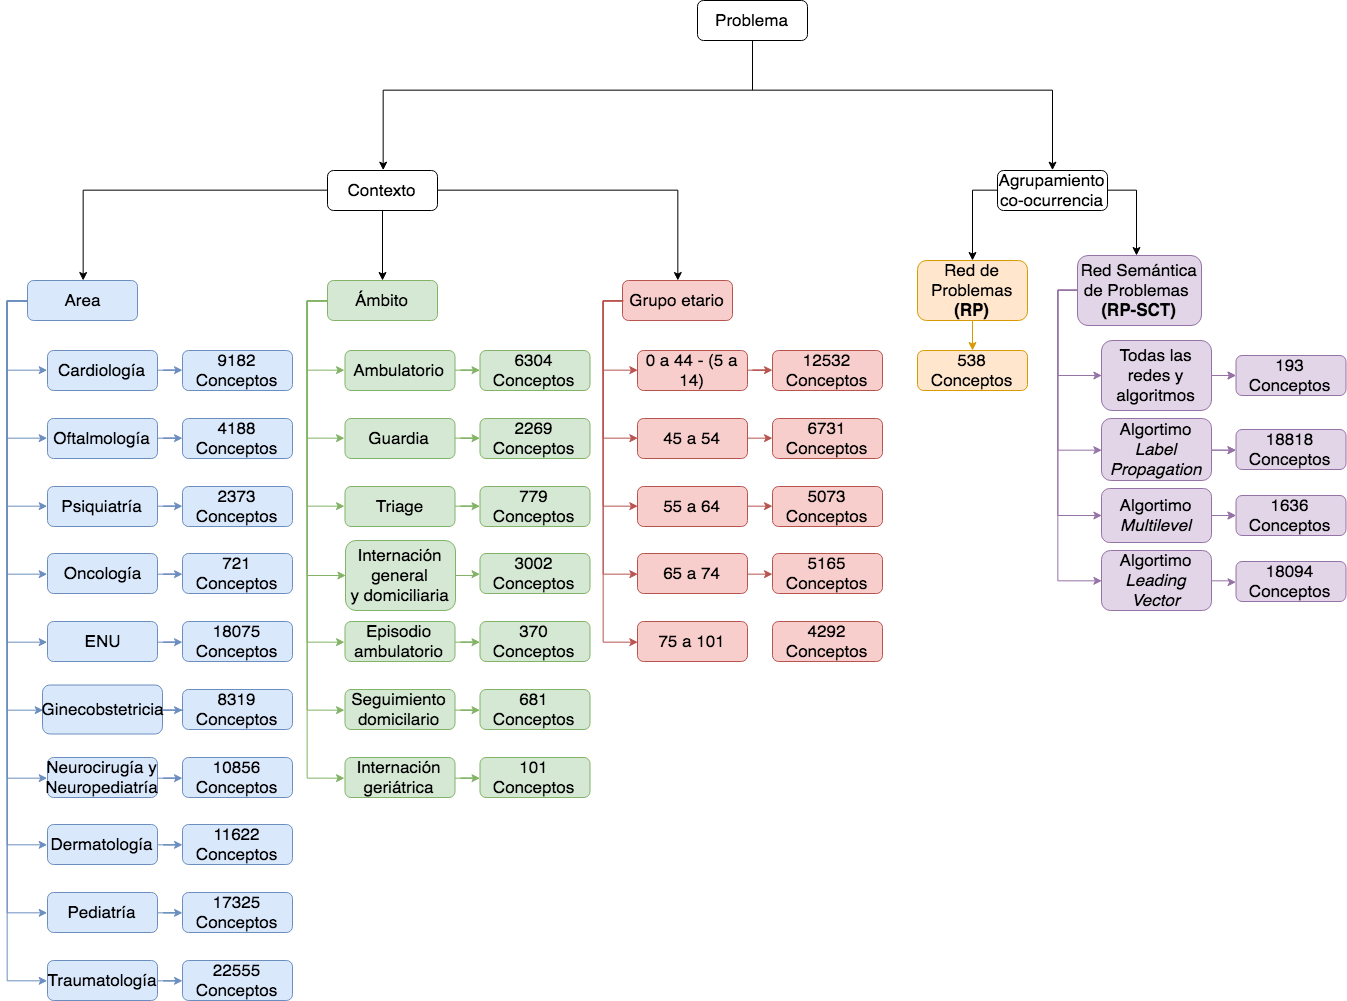
\includegraphics[width=\textwidth]{TaxonomiaProblemas}
\end{figure}

La figura \ref{fig:clust_todo} representa los grupos de la lista de problemas. Mayoritariamente se pueden observar tres grupos, uno azul, otro verde y otro naranja. También mayoritariamente hay una nube densa de nodos fuertemente conectados en el centro, y pequeños grupos se diferencian de ese centro, sin embargo sólo uno de esos pequeños grupos tienen nodos de colores diferente al azul, verde y naranja.

Haciendo el análisis por contexto, el número de nodos disminuye y su comportamiento varía de contexto a contexto. Por el análisis de la sección anterior, se sabe que los servicios de atención a la salud tienen mejor capacidad predictiva de la lista de problemas sin contexto. Haciendo la comparación visual de los grafos que representan las agrupaciones en los servicios de atención de salud, se pueden realizar las siguientes observaciones:

\begin{enumerate}
\item Los grafos con mejor capacidad predictiva son los representados con las figuras \ref{fig:clust_area_pedia} (Pediatría), \ref{fig:clust_area_neuro} (Neurología) y \ref{fig:clust_area_cardio} (Cardiología), a su vez son los grafos más grandes y con mayor variedad de agrupaciones (colores) diferentes en los nodos. Cuando el algoritmo tiene en cuenta el contexto, la lista de predicciones se reduce sólo a los conceptos más cercanos en el mismo grupo.
\item El grafo representado por la figura \ref{fig:clust_area_ENU} que corresponde a los servicios de endocrinología, nefrología y urología, tiene mejor capacidad predictiva en los servicios de endocrinología y nefrología, que en urología. Este es un grafo donde hay muchas conexiones entre los nodos, de ahí su densidad en el centro, y los grupos de nodos que se forman en la periferia tienen relación con los servicios de endocrinología y nefrología y no con urología. Por ejemplo, los problemas asociados a diabetes mellitus, neoplasia de riñón y hematuria.
\item Enfermedad sospechada, dolor y antecedente familiar de trastorno son problemas con un valor de grado muy alto en casi todos los contextos.
\item En el servicio de dermatología, todos los problemas pertenecen al mismo grupo, ver figura \ref{fig:clust_area_dermatologia}. Así mismo es uno de los grafos más pequeños.
\end{enumerate}

Los grafos con el contexto del nivel asistencial o ámbito, permiten hacer las siguientes observaciones:

\begin{enumerate}
\item El grafo más simple es el de la figura \ref{fig:clust_ambito_epi_ambulatorio} (Episodio Ambulatorio), y también el que tiene menor capacidad predictiva.
\item El grafo más complejo es el de la figura \ref{fig:clust_ambito_ambulatorio} (Ambulatorio), pero su capacidad predictiva no es muy diferente a los demás niveles asistenciales.
\item Los grafos de los niveles de asistencia de internación domiciliaria e internación general, son los mismos. Ver figuras \ref{fig:clust_ambito_inter_domici}  y \ref{fig:clust_ambito_inter_general}.

\end{enumerate}
En todos los grafo con el contexto del grupo etario se pueden observar una gran variedad de agrupaciones más pequeñas, que las separan de un centro más complejo y denso de problemas. También se observa una gran variedad de colores, los cuales significan que los métodos de agrupación han encontrado asociaciones significativas entre problemas.

El grafo de la figura \ref{fig:clust_edad_0_4} que representa los problemas entre los 0 y 44 años es el más grande y complejo, y el grafo de la figura \ref{fig:clust_edad_75_101} aunque es el más simple tiene la mejor capacidad predictiva.

\section{Discusión del capítulo}
El objetivo de este capítulo fue realizar un análisis de \textit{graph mining} a la lista de problemas del HIBA con el fin identificar patrones de red y aplicar algoritmos de agrupamiento que permitan encontrar comunidades.

En la identificación de patrones de red se evauaron dos redes: (1) la red formada sólo por los conceptos la lista problemas y sus co-ocurrencias en los individuos \textbf{(\acrshort{RP})}, y (2) extendiendo esta red con sus conexiones jerárquicas $|\textit{ES UN}|$  concepto de Snomed CT \textbf{(\acrshort{RP-SCT})}. La \acrshort{RP} tiene un mejor ajuste a la ley de potencias que la \acrshort{RP-SCT}. Esto debido a que la \acrshort{RP-SCT} tiene una cola mucho más pesada que la \acrshort{RP}. 

El siguiente aspecto evaluado fue los efectos de comunidad en los grafos. La diferencia de las métricas de transitividad y la transitividad local promedio, es que la primera es la medida de la transitividad local en toda la red, en la segunda se calcula por cada vértice la transitividad y los nodos con menos de dos vecinos son considerados como de transitividad cero \cite{Watts1998}. Las diferencias encontradas en  estas dos métricas en las dos redes, indican una alta presencia de nodos que no forman tríadas. Aunque los valores de la longitud media del camino mínimo entre nodos entre las dos redes es similar, para un alto coeficiente de agrupamiento como es el caso de \acrshort{RP} el efecto es que la mayoría de los nodos que son homogéneos se encuentran en pocos saltos dentro de la red, este efecto es similar al fenómeno de mundo pequeño en las redes sociales \cite{Cook2006}. 

Se evidencia que la \acrshort{RP} tiene estructuras más fuertes que la \acrshort{RP-SCT}, además que los nodos están más conectados (promedio grados más altos y longitudes medias más pequeñas). 

Para detectar comunidades se usaron los  algoritmos de agrupamiento \textit{leading vector}, \textit{label propagation} y \textit{multilevel}. Las características de estos algoritmos son diferentes y presentadas en el capítulo 2 (Ver sección \ref{par:aprendizaje_nosupervisado}). La complejidad de estos algoritmos permite que puedan ser empleados en redes de larga escala y con grafos que no están conectados. Según los resultados obtenidos en la modularidad, \textit{Leading vector} es un algoritmo divisivo cuya modularidad se ve afectado por el tamaño del grafo y \textit{label propagation} va obteniendo mejores modularidades en la medida que crece el grafo. El algoritmo {multilevel} es el que mejores modularidades tiene y el número de grupos permanece constante sin importar que se modifique el tamaño del grafo.

Para evaluar la capacidad predictiva de los grupos obtenidos usé los datos de la lista de problemas en el año 2017. Lo que evalué era si había coincidencia en los 10  problemas más cercanos por medidas de centralidad o por distancia semántica. Los problemas más cercanos debían coincidir en el mismo grupo de los que están en la lista de problemas del paciente. Las medidas estadísticas que usé fueron precisión y exactitud. 

Cuando las predicciones son exactas, los resultados con precisiones más altas se logran con 20 nodos excluidos en grados, cercanía y autovector. En el caso de intermediación aumenta en la medida que más se filtren datos, con un máximo local en 400 nodos. Esto es por la relación entre falsos positivos y verdaderos positivos,  donde los filtros por grado, cercanía y autovector tienen mejores resultados por que tienen menos falsos positivos, y en el caso de la intermediación por que tienen más verdaderos positivos. 

En el caso de las mediciones sin repeticiones se observa una exactitud similar en todos los experimentos y que hay una mejora no significativa en la precisión. A diferencia de los experimentos con repeticiones donde se obtiene una exactitud máxima de \num{0,397}, en el caso de los experimentos sin repeticiones la exactitud máxima es de \num{0,255}, esto se debe a que los verdaderos negativos cuentan con muchas repeticiones, en algunos casos reduciéndose a más de la mitad.

En el caso del ordenamiento por distancia semántica  los resultados mejoran  en la precisión incluso sin realizar ningún filtro por medidas de centralidad, pero en cuanto a la medida de exactitud, se obtienen mejores resultados en el ordenamiento por centralidad. Por lo tanto, las medidas de centralidad permite identificar mejor los verdaderos negativos que las distancias semánticas.

Cuando las predicciones no son exactas, sino que se toma como verdadero positivo si al menos hay una distancia de hasta 2 nodos entre la respuesta y las predicciones, hay un incremento significativo de los verdaderos positivos. Por lo tanto, los valores de precisión y exactitud aumentan, presentándose los máximos en los casos en los que no se excluyen nodos.  El mejor resultado se encuentra en el ordenamiento por distancia semántica de menor a mayor, con y sin repeticiones, los valores son  P@10(\num{0,995}) y Acc@10(\num{0,995}) con repeticiones y P@10(\num{0,997}) y Acc@10(\num{0,723}).  Aunque con las predicciones con distancias menores o iguales a 2 nodos, se obtienen precisiones y exactitudes por encima del \num{0.900} se requiere de un análisis más detallado para evaluar si las predicciones son realmente verdaderos positivos. 

El comportamiento diferente en los casos de intermediación se debe a que a diferencia del grado, cercanía y autovector, la intermediación no es una medida de cercanía, su valor está dado porque conecta otros pares de nodos. La interpretación es que al eliminar estos nodos entonces se eliminan los problemas que hacen parte de los síntomas subyacentes, pero no los problemas principales.

Las visualizaciones permiten explicar la razón de las mejoras en las métricas de los contextos de servicios de atención y del grupo etario. Se puede observar que a diferencia de los otros contextos, aquellos en los que se conserva complejidad (por el número de nodos y enlaces) y variedad de grupos (color en los nodos), tienen mejor capacidad predictiva que aquellos que se reducen mucho en tamaño o que tienen pocos grupos. Utilizando el contexto, la precisión máxima P@10 es del \num{0.942} y la exactitud máxima A@10 es de \num{0.943} con repeticiones, y  P@10 de \num{0.948} y A@10 de \num{0.948} sin repeticiones. Estos valores fueron obtenidos en el contexto del grupo etario entre 75 y 101 años, son pacientes que por sus características tienen muchas enfermedades crónicas y varios registros en sus lista de problemas. 

\section{Conclusión del capítulo}
En este capítulo se analizaron los grafos creados a partir de la lista de problemas, sus conexiones con Snomed CT (Red \acrshort{RP}) y la co-ocurrencia en los pacientes (Red \acrshort{RP-SCT}).

El primer análisis fue evaluar diferentes patrones de redes en estos grafos. Concluí que los grafos tienen un mejor ajuste a la ley de potencias que a otras distribuciones y que se evidencian efectos de comunidad. La utilidad de modelar la lista de problemas como un grafo radica en la posibilidad de detectar comunidades significativas que permitan realizar clasificaciones, detectar nodos influyentes y recuperar otros nodos del grupo usando algún criterio de proximidad o semejanza.

En la detección de comunidades significativas se aplicaron los algoritmos de agrupamiento \textit{Leading vector}, \textit{Multilevel} y \textit{Label Propagation}, en la red de problemas \acrshort{RP-SCT} que se encontraban en al menos 5, 10, 100, 1000 y 10 000 pacientes con registros antes de diciembre de 2016 y la red \acrshort{RP}. Esto tenía el propósito de encontrar comunidades que se repitieran a pesar de los enfoques diferentes de los algoritmos y de los tamaños de los grafos. 

Los resultados permitieron encontrar comunidades de problemas, problemas que se detectaron como atípicos debido a su distancia semántica con los otros miembros del grupo, y asociaciones novedosas entre problemas semánticamente distantes.  Los resultados también permitieron detectar grupos de problemas con un contexto similar en la red \acrshort{RP}: Ej. Enfermedades generales (cluster\_6), enfermedades relacionadas con la edad avanzada (cluster\_27), enfermedades relacionada al embarazo (cluster\_16), etc. Mientras que en la red \acrshort{RP-SCT} se encontraron en su mayoría grupos pequeños pero que presentaban asociaciones entre pares de conceptos distantes semánticamente según su clasificación en la ontología de Snomed CT, sin embargo al realizar una búsqueda bibliográfica encontré incidencias de la co-ocurrencia de estas enfermedades en pacientes.

El siguiente paso dentro de la metodología fue evaluar la capacidad predictiva de las comunidades encontradas. Para lo cual en el caso de los pacientes con registros en el 2017, tomé la lista de problemas hasta el 2016 para crear la \textit{query} que permita para generar una lista de predicciones a partir de su co-ocurrencia en las comunidades. La lista de predicciones es de tamaño 10 y su ordenamiento es por la medidas de centralidad o de distancias semánticas. También evalué filtrar de la lista los nodos con mayores medidas de centralidad: grado, intermediación, cercanía y autovector. Las métricas evaluadas fueron precisión P@10 y exactitud Acc@10, tanto en predicciones exactas o si la distancia entre el problema del 2017 y la lista de predicciones es menor a 2 nodos. Los resultados de estos experimentos dieron valores muy bajos, especialmente en el caso de las predicciones exactas donde la mayoría no supera en precisión el \num{0.100} y en exactitud el \num{0.300}.

En la última sección, se filtraron las listas de sugerencias usando los \acrshort{refset} de los contextos del área jerárquica, nivel asistencial y grupo etario. Las métricas mejoran significativamente en cada caso. En menor grado en el nivel asistencial donde los valores de precisión y exactitud se duplican, en promedio son P@10=\num{0.150} y Acc@10=\num{0.500} en las predicciones exactas. Y en mayor grado el servicio de atención de salud y grupo etario. En estos últimos, algunos casos superan \num{0.900} en precisión y exactitud y la mayoría es ubica por encima de \num{0.800}.



%%%% Capítulo 5: Conclusiones
\chapter{Conclusiones y futuros pasos}
\section{Conclusiones generales}
En este trabajo he construido una clasificación de los conceptos de la lista de problemas, a partir de la co-ocurrencia de los problemas dentro de los pacientes y su registro asociado significativamente a diferentes contextos: servicio de atención de salud, nivel asistencial o ámbito y grupo etario. El objetivo de estos grupos o clasificaciones es contribuir al mejoramiento de la calidad de la lista de problemas de los pacientes en su completitud, actualización y granularidad, por medio de la recuperación contextual de información y el uso significativo de Snomed CT.

En la actualidad Snomed CT tiene un amplio cubrimiento de diferentes tópicos relacionados a la salud, es usado en muchos países y está traducido en diferentes idiomas. Uno de los aspectos claves en su uso significativo es la creación de \acrshort{refset} o agrupamientos que puedan ser utilizados como vocabularios controlados dependientes de contextos, sin embargo Snomed CT no específica una metodología para la construcción de dichos agrupamientos.

En esta tesis, construí por medio de algoritmos de graphmining tres niveles diferentes de clasificación de conceptos de Snomed CT: Problemas asociados a niveles asistenciales, Problemas asociados a grupos etarios, Problemas asociados a servicios de atención de salud. Las relaciones entre los conceptos de estas clasificaciones están ponderados por su co-ocurrencia entre los pacientes del Hospital Italiano de Buenos Aires.

En el caso de los problemas asociados a servicios de atención de salud, realicé una validación de su cubrimiento con los \acrshort{refset} publicados por el consorcio \textit{Kaiser Permanente}. En el este capítulo repasaré las contribuciones de estas clasificaciones al proceso de la construcción de \acrshort{refset} de Snomed CT, y presentaré algunas ideas sobre el trabajo futuro de esta línea de investigación.

Se aplicaron algoritmos de aprendizaje no supervisado al grafo construido con la red de problemas (\acrshort{RP})  y sus conexiones semánticas son Snomed CT (\acrshort{RP-SCT}). Los grupos que fueron consistentes en diferentes clasificaciones fueron evaluadas. Se midió  la precisión y exactitud de una lista de predicciones de 10 conceptos que intentaba predecir los problemas que fueron registrados a los pacientes en el año 2017, a partir de los registros de su lista de problemas previo a diciembre de 2016. 

Los \acrshort{refset} de contextos permitieron acotar el universo de búsqueda, y mejoraron significativamente las métricas de precisión y exactitud.

El principal logro de esta tesis es la creación de estas agrupaciones, las cuales tienen múltiples aplicaciones entre las que se cuentan: la recuperación de información, el uso significativo de Snomed CT y la creación de \acrshort{refset} con contexto. Espero que estas aplicaciones deriven una mejora a la calidad de la lista de problemas.

\section{Uso significativo de Snomed CT}
El primer objetivo del uso significativo de Snomed CT es mantener actualizada la lista de problemas con diagnósticos actuales ya activos. Los recursos para lograr esto son los \acrshort{refset} contextuales. En esta guía Snomed CT, presenta algunos públicos disponibles que sirvieron para evaluar el cubrimiento de los servicios de atención de salud.\cite{meaningfuluse}

La metodología para la construcción de los \acrshort{refset} de Servicios de atención de salud y la comparación con otros experimentos realizados por nova scotia\cite{nova} fueron presentados en el congreso Medical Informatics Europe 2018.\cite{Avila2018SelectionSubsets.}

Con el desarrollo de esta tesis, concluimos que la construcción de estos \acrshort{refset} mejora significativamente la recuperación de información en la lista de problemas. Ya que la precisión y exactitud mejoró significativamente con el uso de \acrshort{refset} de contexto.

Los servicios del Hospital Italiano de Buenos Aires, son usados por historias clínicas electrónicas de Argentina, Uruguay y Chile. En trabajos futuros, sería muy beneficioso realizar un consenso entre el uso de las listas de problemas de todos estos centros médicos, para establecer una única lista de problemas controlada que además esté ponderada la frecuencia de uso en las bases de datos clínicas. Un trabajo similar fue realizado por Kaiser Permanente, pero el propuesto tendría la validez internacional de los países del cono sur. Como resultado Kaiser Permanente ha liberado una única lista de problemas desde el 2009 para ser usado en todas las clínicas de su consorcio y mantener la interoperabilidad.\cite{Dolin2004KaiserTerminology.}

\section{Distancias semánticas}

Estimar la distancia semántica entre términos es una de las herramientas más ampliamente usadas para el procesamiento y entendimiento de textos. En esta tesis fue usada para cuantificar la distancia entre los términos predichos y los términos de prueba, asumiendo que las distancias de tamaño 2 eran lo máximo aceptable. La distancia fue medida con el camino más corto entre los dos nodos del grafo.

Una línea de investigación que se desprende de esta tesis es mejorar la manera como se calculan la distancias semánticas. Existen varias metodologías propuestas para medir la similaridad entre dos conceptos en una ontología, específicamente los trabajos con Snomed CT se pueden dividir en dos categorías: enfoques basados en conocimiento y enfoques basados en corpus.  \cite{Mabotuwana2013,BenAouicha2016,Sanchez2011,Harispe2014}

El enfoque basado en conocimiento explota principalmente la estructura jerárquica y las relaciones semánticas de la ontología para hacer inferencias sobre el conocimiento. Este enfoque mide la distancia entre conceptos usando técnicas como el camino más corto, conteo de aristas, profundidad ontológica y ancestro común más bajo \textit{(Lowest Common Subsumer)}. La similaridad es determinada como el inverso de la distancia en su forma más simple, o alguna otra función matemática basada en la distancia ontológica.\cite{Mabotuwana2013}

El enfoque basado en corpus usa un gran corpus con textos específicos del dominio para determinar el valor de la información de cada concepto. Este valor se determina por la frecuencia del concepto en el corpus. Los menos frecuentes son vistos como más informativos que los más comunes.\cite{Mabotuwana2013}

No hay una métrica \textit{gold estandar} para determinar la similaridad entre dos conceptos de una ontología. En un trabajo futuro se evaluaran los dos enfoques, dado que se cuenta con la ontología y el corpus de la lista de problemas. Esta línea de investigación tiene  el objetivo de hallar una métrica con cierto nivel de confianza que determine cuándo dos conceptos son clínicamente similares.

\section{Implementación en una Historia Clínica Electrónica}

La implementación de los modelos en la historia clínica electrónica sugiere el completo desarrollo de un proyecto de software. Según los resultados teóricos obtenidos en esta tesis la línea futura tendrá el diseño de un experimento observacional de corte transversal con la implementación siguiendo los siguientes criterios de inclusión: áreas jerárquicas agrupadas por servicios de atención de salud: Cardiología, dermatología, endocrinología, nefrología, neurología, oftalmología, otorrinolaringología, pediatría, pisquiatría y traumatología, donde los valores de P@10 y Acc@10 superan el 0.800. También cuando el paciente pertenece a los grupos etarios: 15-24, 55-64 y 75-101, donde los valores de P@10 y Acc@10 superan el 0.900.

Para el desarrollo de proyectos de software, el departamento de informática del hospital sigue los fundamentos de gestión de proyectos. Se realiza un Project Charter donde se define el alcance, riesgos, la metodología y entregables. También una Estructura de Desglose del Trabajo (EDT) con el cronograma. Por otro lado, el hospital requiere que el Comité de Ética de Protocolos de Investigación (CEPI) avale el protocolo de investigación. 

Una vez se han alcanzado los avales y el proyecto ingresa dentro del portfolio del departamento de informática, se da inicio al análisis, diseño, desarrollo y pruebas. Este ciclo de software se realiza iterativamente usando la metodología ágil scrum. 


%%%% Capítulo 2: Marco Teórico
%%\chapter{Marco Teórico}
%%\section{Introducción}
El \textit{graph mining} se encarga de hacer descubrimiento de conocimiento en estructuras de grafos. El descubrimiento implica tareas de (a) aprendizaje supervisado encontrando patrones que distinguen un conjunto de grafos de otros, y para lo cual se necesita un conjunto de ejemplos positivos y otro conjunto de ejemplos negativos; (b) aprendizaje no supervisado por medio del agrupamiento o \textit{clustering}; y (c) visualización de grafos para representar el conocimiento.

Dentro del área de la salud, la redes son usadas para representar conocimiento médico. El Hospital Italiano de Buenos Aires extiende un grafo dirigido acíclico llamado SNOMED CT como terminología de referencia, con múltiples fines: epidemiológicos, estadísticos, económicos, soporte para la investigación, etc. SNOMED CT es usado también para representar el conocimiento de los problemas de los pacientes, lo que permite pasar de problemas más genéricos a más específicos en una organización jerárquica.

En las primeras secciones de éste capítulo presento los diferentes patrones que son evaluados en el análisis de grafos y de las redes que representan, con el objetivo de hallar comunidades significativas que permitan clasificar la red según la información contextual y detectar outliers.

En la última sección se encuentra las definiciones de lista de problemas del hospital italiano y cómo ésta extiende el modelo de datos de SNOMED CT.

\section{Redes}
\subsection{Definición}
Las redes están presentes en casi cada aspecto de nuestra vida, la tecnología nos ubica en un mundo lleno de redes, y las relaciones físicas o lógicas que establecemos con nuestro entorno constituyen una red en sí misma. Al final de la década del noventa, el avance y popularidad de los computadores cambió la manera como se entendían las redes. La capacidad de los computadores hizo posible acumular grandes bases de datos con estructuras de redes y analizarlas rápida y eficientemente. Esto permitió por primera vez, la comparación de datos de redes reales con los modelos existentes, en particular el modelo ER. Otra influencia importante de la revolución de la computación fue la creación y rápido desarrollo de dos redes enormes: la internet y la World Wide Web (WWW). A continuación presento algunos ejemplos clásicos de redes, aunque en la literatura siguen surgiendo nuevos.

\subsection{Tipos de redes}\cite{Cohen2010}
% * <mariad.avila@hospitalitaliano.org.ar> 2017-07-01T16:52:38.003Z:
% 
% Actualizar a 2017
% 
% ^.

\paragraph{Redes de computadores y la internet:} Los nodos son los computadores y los enlaces son físicos. Existen varios tamaños de redes, desde una simple LAN (local area network), donde generalmente un pequeño número de computadores están conectados entre ellos, hasta WAN (wide area network) redes de áreas geográficas extensas que consisten desde decenas hasta miles de computadores conectados.
 
La internet, como una red compleja, es generalmente estudiada en 2 niveles: (1) a nivel del router, donde cada router es un nodo, y dos nodos físicamente conectados están conectados por un enlace, y (2) el nivel AS (sistemas autónomos), donde cada sistema autónomo es tratado como nodo, y dos ASs que tienen una conexión física están conectados por un enlace.
 
\paragraph{Redes tecnológicas:} Estas redes incluyen las red de energía eléctrica, la red de teléfono y la red de transporte. Muchas de estas redes tienden a estar altamente correlacionadas con el espacio en el cual residen.
 
\paragraph{Redes virtuales tecnológicas y la WWW:} Este tipo de red también está basado en computadores y otras tecnologías, pero los enlaces y algunas veces los nodos en esta red, son lógicos y no físicos. La red más grande y ampliamente conocida es la  World Wide Web (WWW), en ella cada página es un nodo en la red, y cada hiperenlace entre las páginas es un enlace dirigido.
 
\paragraph{Redes sociales:} Contempla las redes con interacciones entre individuos. Estos pueden consistir en redes de amigos o conocidos, relaciones de trabajo o sexuales. Además de su importancia en los estudios sociales, entender la estructura de estas redes es también importante para los epidemiólogos, ya que es por medio de estas redes que las epidemias se propagan.
 
\paragraph{Redes económicas:} Son un tipo especial de red social donde los nodos no son individuos sino compañías, países o industrias y los enlaces pueden ser las relaciones comerciales, empresas que comparten un director, fluctuaciones correlacionadas con rendimiento de las acciones, etc.
 
\paragraph{Redes biológicas:}Este tipo abarca diferentes tipos de redes, las redes biológicas pueden ser lógicas, representando interacciones entre proteínas, entre genes, o entre proteínas y genes. Interacciones entre moléculas en las vías metabólicas de la célula pueden ser vistas como una red. Aunque las interacciones son físicas, los enlaces no son entidades físicas sino la posibilidad de una interacción entre dos moléculas. Otras redes lógicas son las ecológicas predador-presa (donde los nodos son las especies, y los enlaces dirigidos representan la depredación de una especie por la otra). Otro tipo de redes biológicas son las redes biológicas físicas, como el sistema de nervios, las neuronas en el cerebro y la red de venas en un organismo.
 
\paragraph{Redes en física:} En el mundo de los fenómenos físicos, se pueden considerar muchos tipos de redes, tanto redes físicas, como la de materiales de estado sólido donde los átomos están enlazados con su átomo vecino más cercano en la red, y las redes lógicas, como la que representa el panorama energético.

\paragraph{Redes de salud:} A continuación enumero ejemplos del uso de las redes en el área de la salud.
\begin{itemize}
\item La red de enfermedades humanas\cite{Goh2007TheNetwork.} es una red de trastornos y enfermedades genéticas enlazados a su gen que permite explorar el fenotipo y las enfermedades genéticas asociadas, indicando así el origen genético que tienen en común muchas enfermedades. Este proyecto nació en el 2007, y para el 2014 agregaron la red de síntomas a partir de metadata de los encabezados de temas médicos (MeSH) de PubMed. A partir de estas redes han hecho múltiples trabajos que explican la interacción entre enfermedades, interacciones entre proteínas, interacciones de enfermedades con drogas y comorbolidades.
\item La red de medicina\cite{Haaren2013,Barabsi2011NetworkDisease}, bajo la premisa que una enfermedad es rara vez consecuencia de una anormalidad en una sóla parte del sistema, implican que Las redes resultantes típicamente ilustran el impacto y la complejidad de la asociación de las enfermedades, en la cual las enfermedades pueden ser agrupadas y clusterizadas.

\end{itemize}


\section{Graphmining}
La minería de datos se ha convertido en sinónimo de encontrar patrones frecuentes en datos transaccionales, el término más general descubrimiento de conocimiento abarca esta y otras tareas. Descubrimiento o aprendizaje no supervisado en graph mining implica no sólo la tarea de encontrar patrones en un conjunto de transacciones, sino también encontrar la posible superposición de patrones en un gran grafo. Descubrimiento también implica la tarea de clustering, la cual intenta describir todos los datos por medio de la identificación de categorías o clusters que comparten patrones comunes de atributos y relaciones. Clustering también puede extraer relaciones entre clusters, resultando en una organización jerárquica o taxonómica  sobre los clusters encontrados en los datos.\cite{Cook2006}
 
En contraste, el aprendizaje supervisado es la tarea de extraer patrones que distinguen un conjunto de grafos de otros. Estos conjuntos son típicamente llamados los ejemplos positivos y los negativos. Este conjunto de ejemplos pueden contener muchas transacciones de grafos o un sólo gran grafo. El objetivo es encontrar un patrón gráfico que aparezca a menudo en los ejemplos positivos pero no en los ejemplos negativos. Tal patrón puede ser usado para predecir la clase (positiva o negativa) de nuevos ejemplos. \cite{Cook2006}
 
La última tarea en graph mining es la visualización del conocimiento descubierto. La visualización de grafos es la representación de los nodos, enlaces y etiquetas de un grafo de tal manera que los humanos entiendan los conceptos representados por el grafo.\cite{Cook2006}

\section{Grafos}
Los grafos son usados para describir conceptos matemáticos en las redes. Los grafos representan las propiedades topológicas esenciales de una red mediante el tratamiento de ésta como una colección de nodos y enlaces. Este enfoque permite usar herramientas y métodos matemáticos para realizar cálculos en redes complejas cuyas propiedades sean similares a las de un grafo.

Un grafo es un conjunto de pares ordenados $G=(V,E)$ tal que $E\subseteq [V]^{2}$, así cada elemento de $E$ está asociado a un par de elementos (el mismo o distinto) de $V$. Los elementos de $V$ son llamados vértices (o nodos o puntos) de G, y los elementos de $E$ son llamados aristas (o líneas) de G.\cite{Diestel2005GraphTheory,Balakrishnan2000ATheory} 

Si $G(e)={u,v}$, entonces los vértices $u$ y $v$ son los nodos finales de la arista $e$ y se dice que los vértices $u$ y $v$ son adyacentes si $u \neq v$. El grado de un vértice $v$ es el número de $|E(v)|$ de aristas de $v$, es decir el número de vértices adyacentes a $v$. Un vértice de grado 0 está isolado.\cite{Diestel2005GraphTheory,Balakrishnan2000ATheory}

\subsection{Patrones de grafos en redes}\cite{Tang2010}
La mayoría de las redes de gran escala comparten patrones que no se notan en redes pequeñas. Entre todos los patrones, la mayoría de las características más conocidas son: \textbf{distribución libre de escala, efecto de mundo pequeño y fuertes estructuras de comunidad}.

\subsubsection{Distribución libre de escala}\cite{Tang2010}
Muchas estadísticas en el mundo real tiene una típica escala, un valor alrededor del cual las mediciones de la muestra se centran. Por ejemplo, la altura de todas las personas en Argentina, la velocidad de los autos en las autopistas, etc. Pero los grados de los nodos en las redes de gran escala a menudo siguen una distribución de ley de potencia (también conocidas como distribución Zipfian, distribución Pareto). 
 
Una distribución que sigue la ley de potencia es también llamada distribución sin escalas, ya que la forma de la distribución permanece sin cambios, excepto para una constante multiplicativa general cuando la escala de unidades se incrementa por un factor. Esto es
\begin{equation}
p(ax)=bp(x)
\end{equation}
 
Donde $a$ y $b$ son constantes. En otras palabras, no existe una escala característica con la variable aleatoria. La forma funcional es la misma para todas las escalas. La red con una distribución libre de escalas para grados nodales también se denomina \textbf{red libre de escala}.
 
Mientras que para las distribuciones normales, es extremadamente raro que un evento ocurra con una desviación muy lejana de la media, en las distribuciones de ley de potencias la cola es mucho más larga. De tal manera que es común que algunos nodos de la red tengan alto grado mientras que la mayoría tienen pocas conexiones. La razón es que la cola de una distribución de ley de potencias decae polinomialmente. Esto es asintotáticamente más lento que en la distribución normal que lo hace exponencialmente, resultando en un fenómeno de cola pesada. La curva de la distribución de ley de potencias se convierte en una línea si graficamos la distribución en una escala log-log, ya que
\begin{equation}
\log p(x) =-\alpha \log x + \log C
\end{equation}
Esta gráfica es comúnmente usada para verificar si la distribución sigue la ley de potencias. Una estimación más robusta es aproximar la función de distribución acumulativa (cdf), descripta con la siguiente ecuación:
\begin{equation}
F(X\geq x) \propto  x^{-\alpha+1 }
\end{equation}

\subsubsection{Efectos de comunidades}
Informalmente, una comunidad es un conjunto de nodos donde cada nodo es más cercano a otros nodos en su comunidad que a los nodos que están fuera de ella. Este efecto ha sido encontrado especialmente en las redes sociales.\cite{Tang2010}

Los efectos de comunidades pueden ser medidos con diferentes métricas, a continuación describo las que serán usadas en el análisis de la red de la lista de problemas.

\paragraph{Coeficiente de agrupamiento - Transitividad}
La transitividad\cite{Wasserman1994} $C^{\Delta}$ Se calcula como una medida de la proporción de triángulos cerrados en un grafo:
\begin{equation}
C^{\Delta} =3x\frac{\text{número de triángulos}}{\text{número de tripletas conectadas}}
\end{equation}
Esta métrica muestra cuán agrupado es el grafo, ya que representa la probabilidad de que dos nodos estén conectados si comparten un vecino en común. En el contexto de la lista de problemas, si los problemas $P1$, $P2$ ocurren en pacientes que también tengan $P3$, esta métrica representa la probabilidad de que $P1$ y $P2$ ocurran juntas.

\paragraph{Coeficiente de agrupamiento - Promedio}\cite{Saramaki2006,Kaiser2008}
Calcula el promedio del coeficiente de agrupamiento del grafo G. 
El coeficiente de agrupamiento se calcula con la siguiente ecuación.
\begin{equation}
C = \frac{1}{n}\sum_{v \in G} c_v,
\end{equation}

\paragraph{Longitud media del camino mínimo entre nodos}
Calcula la media de la distancia entre los nodos en un grafo.

\subsubsection{Detección de comunidades}
Según Blonde et al.\cite{Blondel2008FastNetworks}, el problema de detección de comunidades requiere la partición de una red en comunidades de nodos densamente conectados, donde los nodos que pertenecen a diferentes comunidades están escasamente conectados. Formulaciones exactas de este problema de optimización son conocidas por ser computacionalmente intratables. En los últimos años se han propuesto muchos algoritmos para encontrar particiones razonablemente buenas de una manera razonablemente rápida, debido al incremento de la disponibilidad de conjuntos de datos con grandes redes y el impacto de las redes en la vida. Se pueden distinguir los siguientes tipos de algoritmos:
% * <mariad.avila@hospitalitaliano.org.ar> 2017-07-01T19:41:32.016Z:
% 
% Mejorar la cita
% 
% ^.
\begin{itemize}
\item \textbf{Divisivos:} Detectan enlaces entre comunidades y las eliminan de la red. 
\item \textbf{Aglomerativos:} Une nodos/comunidades recursivamente.
\item \textbf{Optimización:} Maximiza una función objetivo.
\end{itemize}

\paragraph{Algoritmo: leading eigenvector}\cite{Newman2006FindingMatrices.} 
\begin{itemize}
\item Complejidad: $c|V|^2 + |E|$
\end{itemize} 
El algoritmo Leading Eigenvector para detectar estructura de comunidades fue implementado por igraph usando un algoritmo recursivo que divide la red maximizando la modularidad respecto a la red original. 
 
Los métodos basados en este enfoque han tenido excelentes resultados en test estandarizados. Desafortunadamente, optimización exhaustiva de la modularidad requiere grandes esfuerzos computacionales, incluyendo algoritmos voraces (\textit{greedy}), enfriamiento simulado (\textit{simulated annealing}) y optimización extrema (\textit{EO}). El algoritmo desarrollado por Newman tiene un enfoque diferente, en el cual se reescribe la función de modularidad en términos de la matriz, lo cual permite expresar la tarea de optimización como un problema espectral en el álgebra lineal. Este enfoque lidera una familia de algoritmos rápidos para detectar comunidades que producen resultados competitivos con los mejores métodos previos.
 
\paragraph{Algoritmo: multilevel}\cite{Blondel2008FastNetworks} 
\begin{itemize}
\item Complejidad: ``lineal'' cuando  $|V|$ es aproximadamente $|E|$, el algoritmo sugiere que podría ser cuadrática con los grafos completamente conectados.
% * <mariad.avila@hospitalitaliano.org.ar> 2017-07-01T19:50:42.851Z:
% 
% Definir grafo completamente conectado
% 
% ^.
\end{itemize}
El tamaño típico de las grandes redes como las redes sociales, las redes telefónicas móviles o la web, ahora se cuenta en millones cuando no billones de nodos y en este escala se demanda nuevos métodos para recuperar información a partir de su estructura. Un enfoque prometedor consiste en la descomposición de redes en subunidades o comunidades, las cuales son conjuntos de nodos altamente interconectados. La identificación de estas comunidades es de crucial importancia ya que pueden ayudar a descubrir modulos funcionales desconocidos a priori tales como tópicos en redes de información o ciber comunidades en redes sociales. Ademas, las meta redes resultantes, cuyos nodos son comunidades, pueden ser usadas para visualizar la estructura de la red original.
 
El algoritmo multilevel encuentra particiones con alta modularidad en grandes redes en poco tiempo y despliega una completa estructura de comunidad jerárquica para una red, dando así acceso a diferentes resoluciones de una detección de comunidades. El algoritmo se divide en dos fases que se repiten iterativamente. Asume que se empieza con una red ponderada de $N$ nodos. Primero, se asigna una comunidad diferente a cada nodo de la red. De esta manera, en esta partición inicial hay tantas comunidades como nodos. Entonces, por cada nodo $i$ se considera los $j$ vecinos de $i$ se evalúa la ganancia de modularidad que se obtendría al eliminar el nodo $i$ de esta comunidad y colocarlo en la comunidad $j$. El nodo $i$ es entonces puesto en la comunidad en la cual la ganancia es máxima y positiva. Si no se obtiene una ganancia positiva, entonces el nodo $i$ se mantiene en su comunidad original. Este proceso es aplicado repetidamente y de manera secuencial para todos los nodos hasta que no se puede lograr ninguna mejora.
 
\paragraph{Algoritmo: label propagation}\cite{Raghavan2007NearNetworks.}
\begin{itemize}
\item Complejidad: $|V| + |E|$
\end{itemize}
Cada nodo es iniciado con una etiqueta y en cada iteración del algoritmo, cada nodo adopta la etiqueta que la mayor cantidad de sus vecino tiene, con los enlaces uniformemente rotos al azar. A medida que las etiquetas se propagan a través de la red de esta manera, grupos de nodos densamente conectados constituyen un consenso en sus etiquetas. Al final del algoritmo,los nodos con la misma etiqueta son conectados como comunidad. Las ventajas de este algoritmo sobre otros métodos es su simplicidad y su efectividad en el tiempo. El algoritmo usa la estructura de la red para guiar su progreso y no optimiza alguna métrica específica. Además, el número de comunidades y sus tamaños no son conocidos a priori y son determinados cuando finaliza el algoritmo.
 
Aunque las redes con una sola comunidad satisface el criterio de parada, este proceso de formación de grupos y competencia “penaliza” que todos los nodos adquieren la misma etiqueta en el caso de redes heterogéneas con una estructura de comunidad implícita. En el caso de redes homogéneas que no tienen estructura de comunidades, el algoritmo identifica la red como una sola comunidad.

\subsubsection{Evaluación de estructuras}
En esta sección he descrito algunos algoritmos para la detección de comunidades. En parte, la razón por la cual hay tantas definiciones y métodos, es que no está clara cómo debe ser la estructura de una comunidad en una red real. De tal manera que diferentes métodos han sido desarrollados según las necesidades de sus autores\cite{Tang2010}.

Para poder comparar los diferentes resultados obtenidos con los algoritmos, utilizaré las siguientes estrategias:

\begin{itemize}
\item Cálculo de modularidad
\item Comparación de las comunidades con un gold-standard 
\end{itemize}

\subsubsection{Cálculo de modularidad}
 
Según Newman\cite{Newman2006FindingMatrices.}, una buena división de una red en comunidades no es sólamente en la cual el número de aristas que hay entre los grupos es pequeño, sino en la que el número de aristas entre los grupos es menor al esperado. Sólo si el número de aristas entre los grupos es significativamente más bajo al esperado se puede decir con justificación que se ha encontrado una estructura de comunidad significativa. Equivalentemente, se puede examinar el número de aristas en comunidades y buscar divisiones de las redes en las cuales este número es más alto del esperado, los dos enfoques son equivalentes. Estas consideraciones constituyen una medida basada en un punto de corte para modificar una función de beneficio $Q$ definida como
\begin{equation}
Q =  (\text{Número de aristas en la comunidad}) -  (\text{Número de aristas esperadas})
\end{equation} 

Esta función de beneficio es llamada \textbf{modularidad}. La modularidad de una partición es un valor escalar entre -1 y 1, la cual mide la densidad de los enlaces en las comunidades comparados con los enlaces entre las comunidades\cite{Blondel2008FastNetworks}. Entre más se acerca a 1 indica estructura de comunidades más fuertes, y entre más se acerque a menos -1 indica que los nodos están distribuidos en comunidades a las que no pertenecen\cite{Tang2010}.

\subsection{Análisis de redes}
El análisis de redes involucra una variedad de tareas, a continuación listo las que aplicaré en este trabajo: \cite{Tang2010}:
\begin{itemize}
  \item Análisis de centralidad, ayuda a identificar los problemas “más importantes” en la red. Ayudará a entender la influencia y el poder del problema en la red:
  
\begin{itemize}
\item \textbf{Grado.}
Cuenta el número de conexiones que tiene un nodo. Los problemas con los grados más altos serán los que más ocurren en los pacientes.
\item \textbf{Intermediación (\textit{betweenness}).} Mide el número de veces que un nodo en particular es miembro de los caminos más cortos entre otros dos nodos.
Usualmente, la medida de intermediación está normalizada en el rango de [0, 1], dónde 0 es un nodo desconectado y 1 un nodo por donde pasan todas las conexiones.\cite{Cook2006,Brath2015GraphData}
\item \textbf{Cercanía (\textit{Closeness}).} La cercanía de un nodo mide la distancia promedio a todos los otros nodos. Si pocos nodos son alcanzables, entonces la medida de cercanía es pequeña, al igual si la distancia entre los nodos aumenta. \cite{Cook2006,Brath2015GraphData}.
\item \textbf{Eigenvector.} Dado un nodo suma recursivamente todas las distancias a todos los otros nodos. Entre más centrales sean los otros nodos, el nodo que se está midiendo tendrá mayor centralidad\cite{Brath2015GraphData}.
\end{itemize}
  \item Detección de comunidades. Los problemas dentro de la red forman grupos. Esta tarea identificará las comunidades a través del estudio de estructuras de redes.
  \item Clasificación de redes y detección de outliers. Algunos problemas están etiquetados con información contextual, las cuales son :servicio de salud, ámbito y grupo etario. Por ejemplo, en una red con algunos problemas pocos comunes identificados como del Servicio Cardiológico, ¿es posible inferir otros problemas poco comunes asociados por su co-ocurrencia en los pacientes?
\end{itemize}

\section{Lista de problemas}
\subsection{Historia}
A fines de la década del 60 Weed\cite{Weed1968} publicó sus ideas respecto a los \textbf{Registros Médicos Orientados a Problemas (RMOP)} que permite identificar y monitorear cada problema médico. Esta lista de problemas debería ser una tabla dinámica de contenidos que pueden ser actualizados en cualquier momento. El HIBA implementó su historia clínica electrónica (HCE) en el año 1998, utilizando la lista de problemas como componente estructural, este proyecto desarrollado in-house actualmente permite el registro de toda la información relacionada con la salud de los pacientes para su posterior análisis\cite{Luna2013,luna2003implementacion}. La HCE es una aplicación web, orientada a problemas y centrada en los pacientes, con funcionalidades personalizadas que dependen del ámbito o nivel de asistencia (ambulatorio, internación general, guardia, triage, internación geriátrica, internación domiciliaria, seguimiento domiciliario, episodio externo y episodio ambulatorio)
 
Cuando un paciente llega a atenderse, el flujo de trabajo de la atención médica requiere que los profesionales ingresen los problemas mediante una línea de texto libre. Durante la implementación de la HCE y la capacitación de los médicos se definió claramente el concepto de \textbf{problema}, que consiste en motivo de consulta o diagnóstico que
genere una acción por parte del sistema de salud\cite{lopez2004codificacion}. Desde 1998 hasta el año 2017 se cargaron más de \num{1700000} textos libres distintos en la lista de problemas de la HCE del HIBA, agrupados en \num{580000} conceptos.

El texto narrativo no estructurado es aún hoy la forma de documentación más frecuentemente usada en medicina y por medio de la codificación del mismo se intenta disminuir la ambigüedad propia del texto libre. Los motivos por los cuales se codifica son múltiples tales como el económico (para facturar un acto médico), epidemiológico o estadístico (para tener datos sobre incidencia y prevalencia de patologías en una población dada), soporte para la investigación (permite la recuperación de información para estudios científicos), asistencial (permite reclutar candidatos para programas de disease management) y por supuesto en el contexto de una HCE es útil para el funcionamiento de sistemas de soporte clínico en la toma de decisiones\cite{lopez2004codificacion,lopez2002creacion}. 

El proceso de la codificación se realiza de manera secundaria y centralizada, a cargo de un número reducido de profesionales de la medicina que concentran el conocimiento de la clasificación a utilizar y son los responsables de asignar secundariamente los códigos correspondientes a las rúbricas de texto libre que el personal asistencial registra durante la atención. Esta modalidad asegura una mejor consistencia en la codificación\cite{lopez2004codificacion,lopez2005desarrollo}.

\subsection{Snomed CT}
\textit{Snomed} es una nomenclatura desarrollada por el Colegio Americano de Patólogos para describir morfología y anatomía, desde el año 1965 ha evolucionado en diferentes versiones, hasta \textit{Snomed RT} cuyo desarrollo estaba basado en lógica. Esta última versión se unió en el año 2002 a \textit{Clinical Terms Version 3} desarrollada por el sistema de salud inglés, dando origen a \textit{Snomed CT} por \textit{Clinical Terms}. En 2007, la \textit{International Health Terminology Standards Development Organisation (IHTSDO)} adquirió los derechos de propiedad intelectual sobre todas las versiones de Snomed. Aunque en un principio se tratara de una nomenclatura sistematizada de medicina, en la actualidad es la terminología más completa y precisa del mundo. \cite{Bhattacharyya2016SNOMEDIHTSDO}

\textit{Snomed CT} permite el almacenamiento y la recuperación de información clínica basados en su significado, la definición de la información se construye a partir de relaciones semánticas\cite{Rector,Bhattacharyya2016,ihtsdo2016SG}. Cuando un sólo concepto no es suficiente para definir la información, se puede crear uno nuevo siguiendo las especificaciones de representación composicional, a esto se le llama post-coordinación. El Hospital Italiano de Buenos Aires extendió a Snomed CT a partir del año 2002, al año \num{2017} cuenta en su sistema terminológico con \num{520000} conceptos post-coordinados y \num{60000} mapeados directamente (pre-coordinados) . Una de sus grandes ventajas es su gran tamaño y cubrimiento, pero a su vez es el principal obstáculo para su uso y mantenimiento.

\subsection{Componentes de Snomed CT}
El modelo lógico de SNOMED CT define la manera en la cual cada componente  y sus derivados están relacionados. Los tipos de componentes son conceptos, descripciones y relaciones. El modelo lógico especifica una representación estructurada de los conceptos usados para representar las entidades clínicas, las descripciones  que son usadas para representar las diferentes variaciones léxicas del concepto, y las relaciones entre los conceptos.\cite{ihtsdo2016SG}

\paragraph{Conceptos:}
Cada concepto representa una única entidad clínica, la cual está referenciada a un identificador único, numérico y fácilmente procesable por un computador. El identificador provee una referencia única y sin ambiguedades a cada concepto y no tiene tiene ninguna semántica.\cite{ihtsdo2016SG}

\paragraph{Descripciones:}
Un conjunto de descripciones textuales son asignadas a cada concepto. De esta manera el humano obtiene una representación del concepto en su lenguaje natural.

\paragraph{Relaciones:}
Una relación representa una asociación entre dos conceptos. Las relaciones son usadas para definir lógicamente el significado de un concepto de tal manera que pueda ser procesada por un computador. Hay dos tipos de relaciones:

\begin{enumerate}
\item Relaciones subtipo: Usa la relación $|\text{is a}|$, de tal manera que el concepto $P$ $|\text{is a}|$ $Q$,  define que el concepto $P$ es un subtipo de concepto $Q$, o de manera inversa que $Q$ es un supertipo de $P$
\item Relaciones atributos: Una relación atributo contribuye a la definición del concepto mediante la asociación con otros valores que permiten la caracterización del concepto, estos valores pueden ser estructuras corporales, sustancias, objetos físicos, etc.
\end{enumerate}

Diseccionado la estructura esquemática de Snomed Ct, cada concepto es representado con un nodo en el grafo y cada relación entre los conceptos es representada por una arista. No hay relaciones circulares y todas son unidireccionales sin excepciones, pero un concepto $P$ puede tener más de una relación de salida o concepto $Q$.\cite{Bhattacharyya2016}.

\subsection{Modelo de Conceptos de Snomed CT}
Los conceptos de Snomed CT tienen una organización jerárquica, en la forma de un grafo dirigido acíclico, lo que permite pasar de conceptos más genéricos a más específicos en grados de granularidad\cite{Bhattacharyya2016}. El modelo especifica la forma en que los conceptos están dispuestos dentro de los subtipos de jerarquía y los tipos de relaciones de atributos que se permiten en los conceptos que pertenecen a dicha jerarquía \cite{Bhattacharyya2016,ihtsdo2016SG}. Como consecuencia, cada concepto debe pertenecer a una sola jerarquía.
% * <mariad.avila@hospitalitaliano.org.ar> 2017-07-02T20:04:44.802Z:
% 
% > grafo dirigido acíclico
% Definir grafo dirigido acíclico en grafos
% 
% ^.
 
Hay 19 jerarquías, no todas son usadas para representar conceptos clínicos. Las siguientes 8 jerarquías tienen reglas para definir atributos y crear conceptos clínicos según IHTSDO\cite{ihtsdo2016EG}.

\begin{itemize}
\item \textbf{Hallazgo clínico}, representa los resultados de una observación clínica, evaluación o juicio e incluye estados clínicos normales y anormales. La jerarquía de hallazgo clínico incluye conceptos para representar diagnósticos.
\item Los\textbf{ procedimientos} representan actividades realizadas en la prestación de servicios de salud. Incluyen no sólo los procedimientos invasivos sino también la administración de medicamentos, toma  de imágenes, educación, terapias y procedimientos administrativos.
\item Los \textbf{especímenes} representan entidades que son obtenidas (usualmente de pacientes) para el análisis.
\item \textbf{Estructuras corporales}, representan estructuras anatómicas normales y anormales.
\item \textbf{Productos biológicos/farmacéuticos}, representan productos farmacéuticos (no dispositivos)
\item Las \textbf{situaciones de contexto explícito} representan conceptos en los cuales el contexto clínico es especificado como parte de una definición del mismo concepto. Esto incluye la presencia o ausencia de una condición, ya sea que el hallazgo clínico es actual, hace parte del pasado o está relacionado a alguien diferente al paciente.
\item Los \textbf{eventos} represente las ocurrencias que excluyen a los procedimientos y las intervenciones.
\item Por último, los \textbf{objetos físicos }representan a los objetos naturales o hechos por el hombre.
\end{itemize}
 
La tabla \ref{jerarquiasLista} contiene las jerarquías que son usadas en la lista de problemas y la frecuencia de conceptos, se puede observar que las jerarquías más usadas son Hallazgo Clínico, Situación con Contexto Explícito y Procedimientos.

% Please add the following required packages to your document preamble:
% \usepackage{booktabs}
\begin{table}[htb]
\centering
\caption{Jerarquías de la lista de problemas}
\label{jerarquiasLista}
\resizebox{\columnwidth}{!}{%
\begin{tabular}{@{}lll@{}}
\toprule
Jerarquía & Cantidad de Problemas & Conceptos diferentes \\ \midrule
HALLAZGO CLÍNICO & 13594650 & 82732 \\
SITUACIÓN CON CONTEXTO EXPLÍCITO & 1222531 & 5086 \\
PROCEDIMIENTO & 1138167 & 14991 \\
OTRAS JERARQUÍAS & 144553 & 1122 \\
EVENTO & 40084 & 298 \\
ESTRUCTURA CORPORAL & 11274 & 186 \\
PRODUCTO BIOLÓGICO/FARMACÉUTICO & 2040 & 35 \\
OBJETO FÍSICO & 1285 & 75 \\ \bottomrule
\end{tabular}
}
\end{table}

\subsection{Reference sets}
Para facilitar el uso de SNOMED CT se construyen \textit{reference set (refset)}, los cuales agrupan los conceptos en determinados dominios como especialidades, cohortes, tipos de enfermedades, etc. Estos dominios son llamados subset simples.

SNOMED CT no define metodologías para construir refset con conceptos que se agrupen por un contexto, la metodología propuesta es agrupar los conceptos usados en el histórico de la lista de problemas según el contexto dado por el área jerárquica, el grupo etario y el nivel de asistencia con el que fue registrado.

A continuación, en la tabla \ref{refsetsSnomed} presento la lista de refset disponibles por las organizaciones que tienen listas públicas de problemas que agrupan conceptos en las dimensiones que se analizaron en esta tesis, para compararlas como estándar.

\begin{table}[htb]
\caption{Reference Sets disponibles como estándar}
\label{refsetsSnomed}
\begin{tabularx}{\textwidth}{@{}XXX@{}}
\toprule
Organización & Descripción & Refset disponibles \\ \midrule
Kaiser permanente (US) & En el 2010, anunció la donación de su Convergent Medical Terminology (CMT). Esta donación contiene el conjunto de conceptos más usados en ciertos dominios. Kaiser permanente es un consorcio que integra 28 centros médicos y tiene presencia en 8 estados, es la organización más grande de cuidado médico en Estados Unidos. & Cardiology; Common Lab Procedures; Emergency Department; Endocrine,  Nephrology, and Urology; ENT, Gastroenterology, and Infectious Diseases; Hematology and Oncology; History and Family History; Injury; Mental Health; Miscellaneous Problem List ; Musculoskeletal; Neurology; Obstetrics and Gynecology; Ophthalmology; Orthopedics; Pediatrics; Primary Care; Radiology; Skin/Dermatology and Respiratory; Specimen Source and Specimen Type; Urology \& Nephrology; Vaccinations; Vascular Procedures List \\
% National Health Service (UK) & El servicio nacional de salud provee en línea\footnote{https://dd4c.digital.nhs.uk/dd4c/} una base de datos con todos los subsets creados por UK Terminology Centre. Los Subsets disponibles están basados en especialidades o hacen parte de requerimientos nacionales& +400 subsets simples \\ 
\bottomrule
\end{tabularx}
\end{table}

\section{Resumen}
En este capítulo he presentado el graph mining y el conjunto de técnicas que usaré para analizar la red que representa el conocimiento médico en SNOMED CT: (a) análisis de centralidad, (b) detección de comunidades y (c) clasificación y detección de outliers.

Expliqué cuáles son los componentes y el modelo lógico de SNOMED CT, el cual tiene una estructura jerárquica. Este capítulo permitió detectar que la lista de problemas se concentra principalmente en 4 jerarquías de las 19: Hallazgo clínico, Situación con contexto explícito, Procedimiento y Eventos, los conceptos que estén por fuera de estas jerarquías se interpretan como ruido.
Gracias al estudio del estado del arte definí también que la metodología de aprendizaje no supervisado que  permite agrupar conceptos en un contexto, puede usarse como una metodología replicable para generar \textit{refset} de SNOMED CT.

En los siguientes capítulos usaré las definiciones presentadas en éste, para caracterizar la red de la listar de problemas y crear comunidades según el contexto. Mi trabajo se centra en este punto, contribuyendo a la organización de los datos y a la creación de servicios para recuperar conceptos dentro de un contexto.


%%%% Capítulo 3: ETL
%%\chapter{Descripción y limpieza de los datos}
%%\section{Introducción}
En este capítulo describiré el conjunto de datos de la lista de problemas, cómo ha sido su distribución en el tiempo y seleccionaré algunos elementos del contexto: (a) área jerárquica del especialista, (b) grupo etario del paciente y (c) nivel de asistencia, para evaluar en el siguiente capítulo si inciden en los problemas médicos que son registrados. 

También describo los procesos de ETL que realicé para que los experimentos fuesen comparables con los realizados en otras instituciones.

El proceso más complejo fue la reducción de la cardinalidad de las áreas jerárquicas, que pasaron de ser 918 a 29 servicios de atención de salud mapeados a servicios de SNOMED CT. Los conceptos que se agrupan alrededor de estos servicios de atención son llamados \textit{refsets} por especialidad médica y fueron creados con el histórico de la lista de problemas.

Uno de los aspectos claves en el uso significativo de la terminología es la creación de \textit{refsets} que puedan ser utilizados como vocabularios controlados dependientes de contextos. Estos \textit{refsets} facilitan el uso de SNOMED CT como terminología de codificación primaria para la lista de problemas u otros niveles de documentación clínica, y maximizaran potencialmente la interoperabilidad de datos a través de las instituciones\cite{Dolin2004KaiserTerminology.}.

Para la construcción de estos \textit{refsets} se siguen dos metodologías, determinar por extensión cuáles son los conceptos que los componen, ya que no es fácil realizar la restricción por una jerarquía o partes de ella \cite{Hjen2014MethodsSets.,Lee2013AImplementations.}; o la generación automática y el uso de \textit{refsets} públicos para comparar el cubrimiento de su contenido \cite{Lee2013AImplementations.}. Este tesis usa la segunda metodología y evalúa el cubrimiento con Kaiser Permanente CMT.

\section{Comprensión de datos}
La lista de problemas registra las observaciones y hallazgos realizados a los pacientes y otra informacion del contexto. Los problemas de los pacientes son descripciones que se agrupan en conceptos, y los conceptos a su vez pertenecen a uno o varios \textit{refsets}.
Cuando se registra un problema, se asocia el área jerárquica del usuario que ingresó el problema.

El conjunto de datos además tiene el atributo nivel de asistencia que indica el ámbito en el que fue cargado el problema (1 = Ambulatorio , 2 = Internacion General, 3 = Guardia, 4 = Triage, 5 = Internacion Geriatrica, 6 = Internacion Domiciliaria, 7 = Seguimiento Domiciliario, 8 = Episodio Externo, 9 = Episodio Ambulatorio). La figura \ref{fig:ModeloER} contiene el modelo entidad relación, donde se muestra cómo se relacionan estos datos.

\begin{figure}[ht]
\caption{Modelo Entidad-Relación de lista de problemas}
\label{fig:ModeloER}
\centering
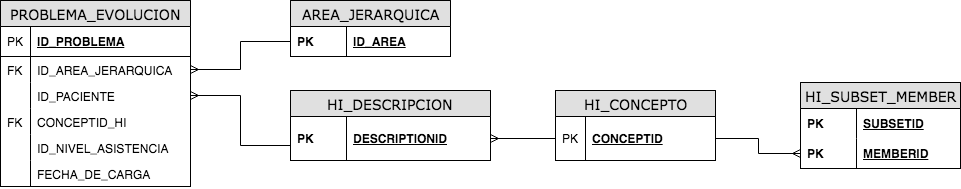
\includegraphics[width=0.9\textwidth]{ER_Problemas}
\end{figure}

\subsection{Distribución en el tiempo}
El atributo FECHA\_DE\_CARGA indica la fecha en la que se cargó el problema por primera vez, las posteriores veces se vuelve a usar el problema registrado y no se crea uno nuevo. En la figura \ref{fig:registrosYConceptos}, se puede observar que aunque la implementación de la HCE empezó en el año 1998, hay registros anteriores a esa fecha los cuales se interpretan como errores en el momento de la carga, al igual que los registros con las fechas superiores al 2017. En total son \num{9149} casos que corresponden al \num{0,004}\% de los datos.

Como se muestra en la figura \ref{fig:registrosYConceptos} la distribución no es uniforme, su crecimiento se explica por los hitos de implementación dentro de la HC, en el año \num{2002} se generalizó el uso de la HCE en todo el hospital, y en el año \num{2006} se implementó el servidor de terminología. Los años \num{2015} y \num{2016} muestran un incremento en el registro de la lista de problemas.

En cuanto a los conceptos diferentes registrados por año, se observa una distribución más uniforme, especialmente después del año \num{2007}.Los datos del año 2017 son sólo los del primer semestre.

\begin{figure}[ht]
\caption{Distribución de problemas por año de carga}
\label{fig:registrosYConceptos}
\centering
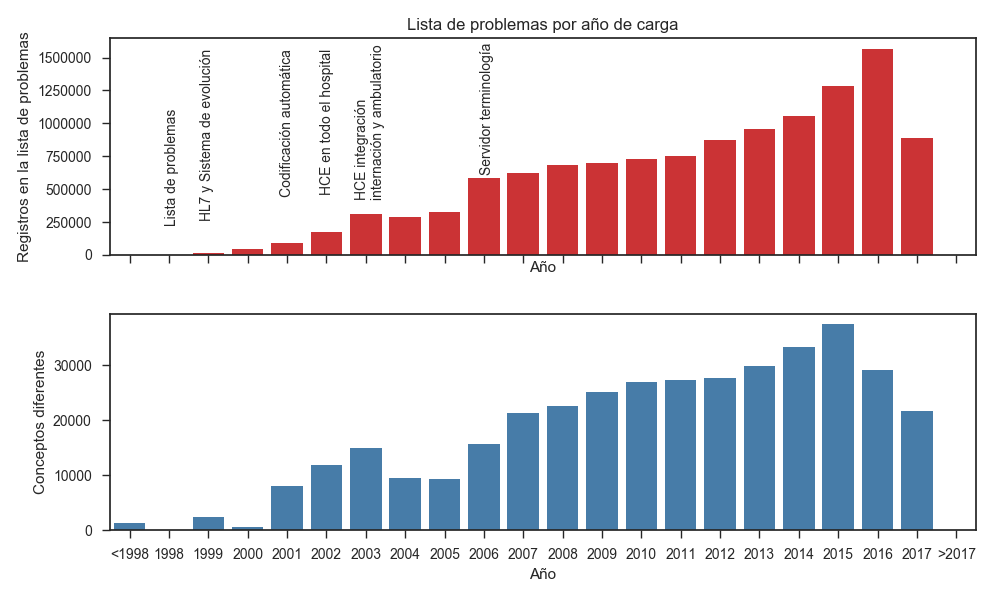
\includegraphics[width=\textwidth]{chart1}
\end{figure}

\subsection{Distribución por individuo}
Según la figura \ref{fig:listaIndividuos} la mayoría de los individuos tiene sólo un problema registrado en su lista de problemas, estos corresponde al \num{34.1}\% de los datos. Los individuos que tienen registrados hasta 10 problemas en la lista son el \num{80}\% de los datos.

\begin{figure}[ht]
\caption{Distribución del tamaño de la lista de problemas por individuos}
\label{fig:listaIndividuos}
\centering
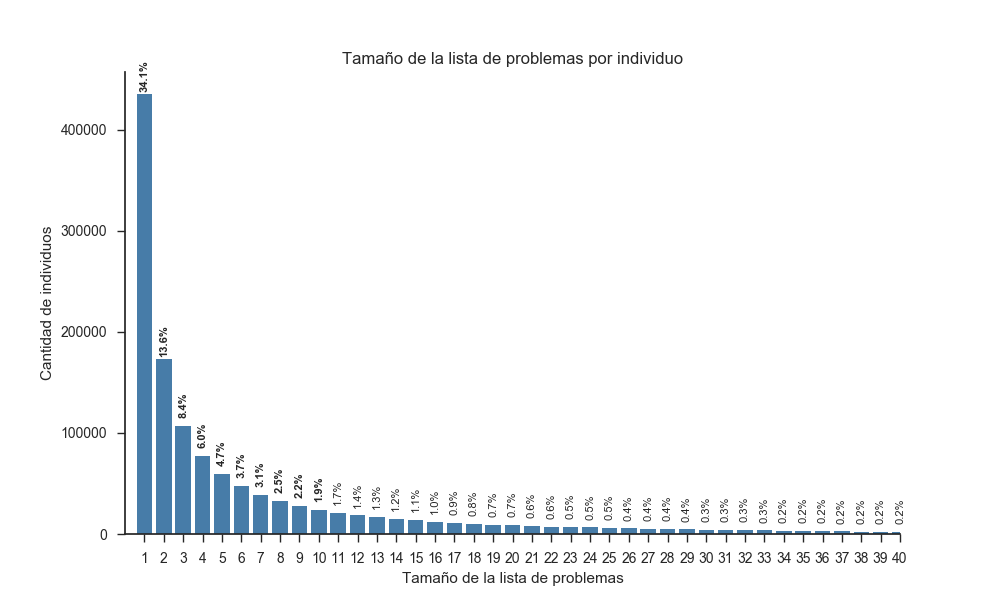
\includegraphics[width=\textwidth]{chart2}
\end{figure}

\subsection{Distribución por conceptos}
El conjunto de datos contiene \num{88869} conceptos distintos usados para identificar problemas de los pacientes. La figura \ref{fig:listaProblemas} representa el uso de estos conceptos dentro de la RMOP, en ella puedo observar que un conjunto pequeño de problemas tiene una frecuencia muy alta y el resto que queda en la cola de la distribución son usados muy pocas veces. Los conceptos más frecuentemente usados son Control de salud, Fiebre, Dolor abdominal,  Hipertensión arterial, Catarro de las vías áreas superiores, Malestar general, Tos, Embarazo, Lumbalgia, Broncoespasmo, Evaluación inicial del paciente e Infección del tracto urinario, que juntos son el \num{20}\% del total de registros. 

El desafío de esta tesis es investigar si hay conceptos que estén correlacionados entre si, que puedan ser útiles para ser sugeridos como parte de la lista de problemas de los pacientes dentro de determinados contextos. 

\begin{figure}[ht]
\caption{Distribución de todos los problema por su aparición en la lista}
\label{fig:listaProblemas}
\centering
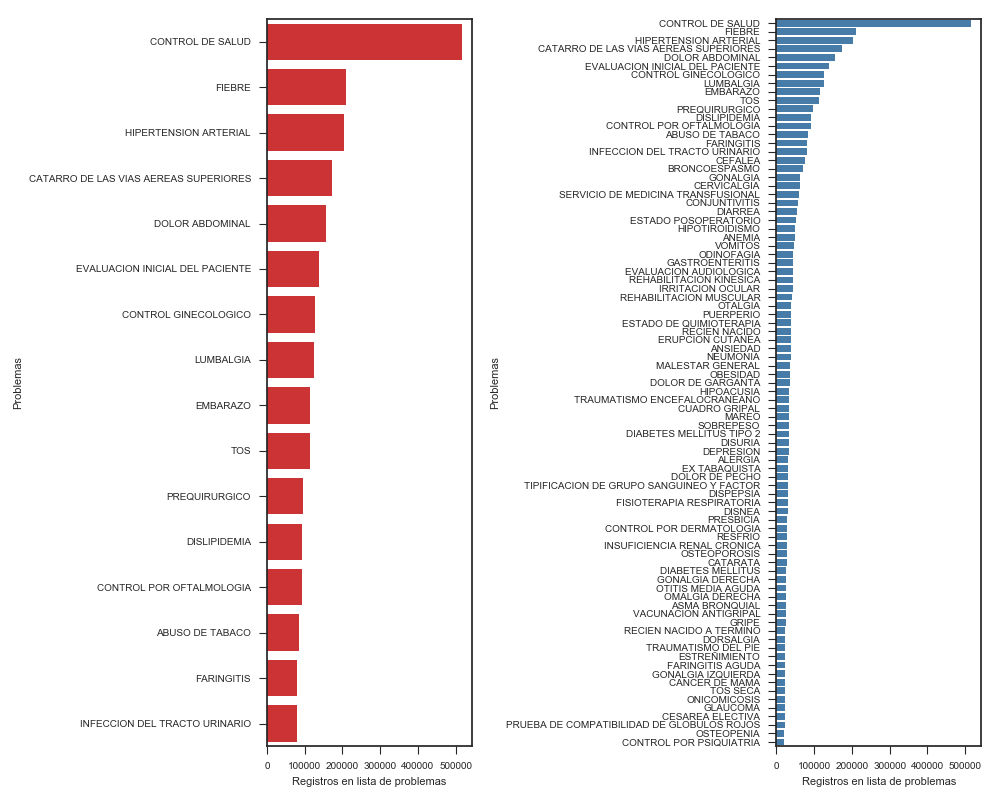
\includegraphics[width=\textwidth]{chart3}
\end{figure}

\subsection{Distribución por contextos}
Los contextos que tuve en cuenta en esta tesis fueron área jerárquica, nivel de asistencia y grupo etario, a continuación describo cómo se distribuyen los conceptos y registros de la RMOP en los contextos.


\subsubsection{Contexto: Área Jerárquica}
La HCE tiene 918 áreas jerárquicas, de las cuales 601 tienen usuarios que han registraron problemas dentro de la lista de algún paciente. Hay dos jerarquías que usan más de \num{20000} conceptos (Clínica médica y Medicina Familiar), el resto de jerarquías usan en promedio menos de 5000 conceptos. 

Las áreas jerárquicas que tiene el HIBA responden a necesidades operativas de la HCE, pero su nivel de disgregación no significa que la lista de problemas necesite también ese nivel de detalle, por el contrario se evidencia al aplicar algoritmos de agrupamiento que hay solapamientos de jerarquías. Con el objetivo de reducir la cardinalidad en las áreas jerárquicas y agruparlas dentro de las más representativas e interoperables, seguí la metodología que se encuentra en la figura \ref{fig:MetodologiaReduccionAreas}.


\begin{figure}[ht]
\caption{Metodología para reducción de áreas jerárquicas}
\label{fig:MetodologiaReduccionAreas}
\centering
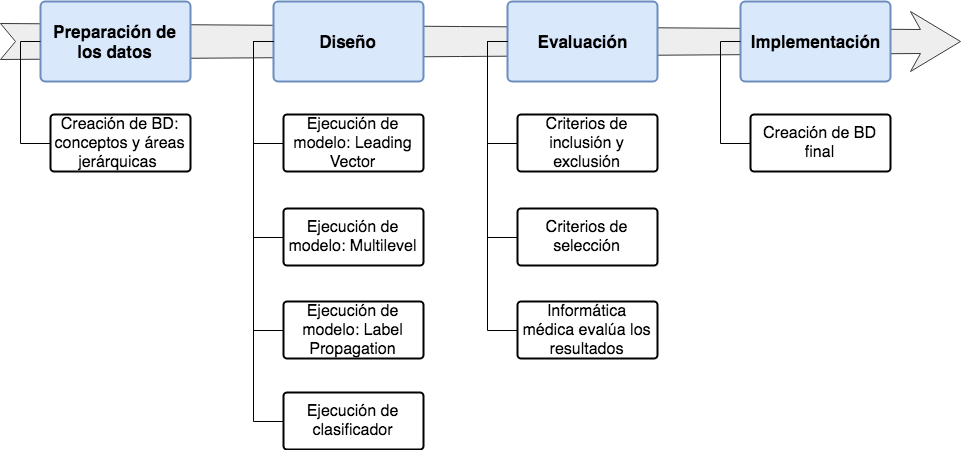
\includegraphics[width=0.9\textwidth]{Reducci_n_cardinalidad}
\end{figure}

En la primera fase de preparación de los datos, cree la base de datos de grafos. En el modelo de datos que se observa en la figura \ref{fig:ModeloDatosAreas} los nodos son los conceptos y las áreas jerárquicas, y las relaciones son las jerarquías (ES\_UN) entre los conceptos y su uso (REGISTRA\_PROBLEMA)  por el área. De tal manera que se represente los diferentes niveles de generalización de los conceptos con la relación (ES\_UN), y que un área jerárquica tiene varios conceptos y un concepto puede estar en varias áreas con la relación (REGISTRA\_PROBLEMA). 

\begin{figure}[ht]
\caption{Modelo de datos}
\label{fig:ModeloDatosAreas}
\centering
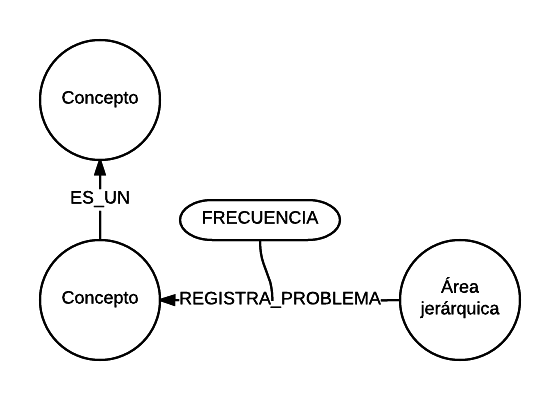
\includegraphics[width=0.5\textwidth]{Modelo_grafo_areas}
\end{figure}

La segunda fase tiene el propósito de encontrar qué áreas jerárquicas comparten similares conceptos, y así identificar las áreas que se pueden agrupar como una sola. En el segundo experimento el propósito es identificar los servicios que se están solapando entre sí, usé un algoritmo de aprendizaje supervisado para predecir el servicio al que pertenecen los conceptos, este algoritmo tiene mayor dificultad para predecir el servicio si hay muchos conceptos similares entre ellos por lo tanto serían candidatos a fusión.

La tercera fase es para evaluar el modelo, se compone de:(a) Informáticos médicos determinan si los criterios se deben aplicar a cada una de las 918 áreas, y (b) Evaluación de la cobertura de los \textit{refsets} formados a partir de los servicios finales.

\paragraph{Fase de diseño:Experimento 1 (Agrupamiento de áreas jerárquicas)}

\subparagraph{Criterios de exclusión}

\begin{itemize}
\item Áreas jerárquicas con sólo un concepto seleccionado.
\item Áreas jerárquicas dentro del cluster de administrativos, las cuales corresponden a usuarios que seleccionaron problemas por razones operativas administrativas y no por razones médicas.
\end{itemize}

\subparagraph{Criterios de selección}
\begin{itemize}
\item Los servicios de la atención de la salud de la jerarquía de SNOMED CT son usados para mapear los del HIBA, de tal manera que los servicios finales permitan la interoperabilidad con otros centros de salud. Para realizar el mapeo, hice una búsqueda en SNOMED CT con string matching del nombre del área del HIBA o del área más general que la contenía.
\item Si no hay un mapeo, seleccioné el servicio de las áreas que están dentro del mismo cluster de label propagation y multilevel, y que además hayan seleccionado los mismos conceptos.
%\item Si al aplicar un algoritmo de clasificación se presenta un alto solapamiento de conceptos entre servicios, estos son candidatos a fusionarse
\end{itemize}

\subparagraph{Diseño del modelo}: Ejecuté 3 algoritmos de agrupamiento. como se observa en la tabla \ref{clusteringAreas}, el algoritmo leading vector dividió el conjunto de datos en 2 y su modularidad es la más baja por lo tanto sus resultados se descartaron.  Los resultados de los otros dos algoritmos fueron usados en los criterios de selección de jerarquía.

\begin{table}[htb]
\centering
\caption{Agrupamiento de áreas jerárquicas y conceptos}
\label{clusteringAreas}
\begin{tabular}{@{}llll@{}}
\toprule
Algoritmo         & Modularidad & Grupos & Test \\ \midrule
Label Propagation & 0.165       & 18     &      \\
Leading Vector    & 0.144       & 2      &      \\
MultiLevel        & 0.447       & 14     &      \\ \bottomrule
\end{tabular}
\end{table}

\paragraph{Fase de diseño:Experimento 2 (Clasificador de áreas jerárquicas)}

\subparagraph{Criterios de selección}
\begin{itemize}
\item Si al aplicar un algoritmo de clasificación se presenta un alto solapamiento de conceptos entre servicios, estos son candidatos a fusionarse
\end{itemize}

\subparagraph{Diseño del modelo}: 
Un enfoque de clasificación permite identificar aquellos servicios que tienen una superposición de conceptos. Usé el algoritmo de aprendizaje supervisado StanfordNLP ColumnClassifier \cite{manning-EtAl:2014:P14-5},  para predecir el servicio al que pertenecen los conceptos, este algoritmo tiene mayor dificultad al predecir el servicio si hay muchos conceptos similares entre ellos.

\paragraph{Evaluación final del modelo}: Ejemplos de los resultados de la aplicación de los criterios de exclusión y de selección del primer experimento se encuentran en la tabla \ref{ejemploCriterios}. Los resultados de la aceptación de estos criterios se encuentran en la tabla \ref{resultadosCriterios}, el \num{63}\% de los casos fueron excluidos correctamente. Con respecto a los criterios de selección, el \num{96}\% de los casos fueron seleccionados correctamente según la evaluación realizada por la residencia médica.

% Please add the following required packages to your document preamble:
% \usepackage{booktabs}
\begin{table}[htb]
\centering
\caption{Ejemplos de criterios de exclusión y selección}
\label{ejemploCriterios}
\begin{tabularx}{\textwidth}{@{}XlXX@{}}
\toprule
Área Jerárquica                                                          & Excluído? & Servicio Seleccionado            & Observaciones                                                     \\ \midrule
Dirección administrativa                                                 & Si        &                                  & Hace Parte Del Cluster De Administrativos                         \\
Coordinación de turnos - departamento de enfermería                      & Si        &                                  & Tiene un sólo concepto seleccionado.                              \\
Servicio de neurocirugía                                                 & No        & Servicio de neurocirugía         & \textit{String Matching} Con un servicio de Snomed CT                      \\
Sección diálisis peritoneal continua ambulatoria- Servicio de nefrología & No        & Servicio de nefrología adultos   & \textit{String Matching} del área más general con un servicio de Snomed CT \\
Rinología plástica                                                       & No        & servicio de otorrinolaringología & Comparte cluster con áreas con los mismos conceptos.              \\ \bottomrule
\end{tabularx}
\end{table}

% Please add the following required packages to your document preamble:
% \usepackage{booktabs}
\begin{table}[htb]
\centering
\caption{Resultados de la aplicación de los criterios de exclusión y selección}
\label{resultadosCriterios}
\begin{tabular}{@{}lll@{}}
\toprule
Criterio                      & Reportados & Aceptados \\ \midrule
Criterio de exclusión         & 223        & 142       \\
Selección por string matching & 291        & 291       \\
Selección por agrupamiento    & 116        & 111       \\ \bottomrule
\end{tabular}
\end{table}

En este primer experimento reemplacé las 601 áreas jerárquicas con 44 servicios de atención médica de SNOMED CT, y eliminé las que entraron en el criterio de exclusión y fueron aceptadas por el residente.

En el segundo experimento, los datos de entrada son los conceptos y los servicios finales del experimento 1. Realizando una partición de 50\% de los datos para crear entrenamiento y 50\% para test, el modelo creado predice a qué servicio pertenecen los conceptos, con los siguientes F1 score:  Accuracy/micro-averaged F1: 0.736, Macro-averaged F1: 0.500.

La matriz de confusión generada por el modelo aporta información sobre qué servicios comparten los mismos conceptos, y propone así una fusión entre ellos. La tabla \ref{serv_aten_hiba} contiene los 44 servicios que fueron mapeados en el experimento 1, y los 29 servicios finales obtenidos a partir del experimento 2. Al crear un nuevo modelo con los mapeos de los servicios del experimento 2, obtengo los siguientes F1 score: Accuracy/micro-averaged F1: 0.775, Macro-averaged F1:0.664

% Please add the following required packages to your document preamble:
% \usepackage{booktabs}
% \usepackage{graphicx}
\begin{table}[htb]
\centering
\caption{Servicios de atención médica del HIBA}
\label{serv_aten_hiba}
\resizebox{\textwidth}{!}{%
\begin{tabular}{@{}lrrlrrl@{}}
\toprule
Servicios Experimento 1 & F1 Score & TP & Servicios Experimento 2 & F1 Score & Solapados & Acción \\ \midrule
servicio de anestesia & 0,048 & 155 & servicio de medicina general & 0,747 & 1595 & Fusionar \\
servicio audiológico & 0,000 & 0 & servicio de otorrinolaringología & 0,675 & 10 & Fusionar \\
servicio de cardiología adultos & 0,672 & 29589 & servicio de cardiología adultos & 0,672 & - & Mantener \\
servicio de cardiología pediátrica & 0,871 & 9531 & servicio de cardiología pediátrica & 0,871 & - & Mantener \\
servicio de cirugía general & 0,598 & 29993 & servicio de cirugía general & 0,598 & - & Mantener \\
servicio de cirugía pediátrica & 0,437 & 3490 & servicio de cirugía pediátrica & 0,437 & - & Mantener \\
servicio de cirugía plástica & 0,664 & 3619 & servicio de cirugía plástica & 0,664 & - & Mantener \\
servicio de cirugía vascular & 0,178 & 406 & servicio de cardiología adultos & 0,672 & 909 & Fusionar \\
servicio de colposcopía & 0,000 & 0 & servicio de ginecoobstetricia & 0,877 & 293 & Fusionar \\
servicio de dermatología & 0,800 & 39370 & servicio de dermatología & 0,800 & - & Mantener \\
servicio de dermatología pediátrica & 0,405 & 2141 & servicio de dermatología & 0,800 & 3240 & Fusionar \\
servicio de endocrinología & 0,687 & 20509 & servicio de endocrinología & 0,687 & - & Mantener \\
servicio de endocrinología pediátrica & 0,518 & 1003 & servicio de endocrinología pediátrica & 0,518 & - & Mantener \\
servicio de enfermería & 0,595 & 5968 & servicio de enfermería & 0,595 & - & Mantener \\
servicio de farmacia & 0,392 & 112 & servicio de medicina general & 0,747 & 186 & Fusionar \\
servicio de fisioterapia & 0,993 & 34731 & servicio de fisioterapia & 0,993 & - & Mantener \\
servicio de fonoaudiología & 0,612 & 7402 & servicio de otorrinolaringología & 0,675 & 6136 & Fusionar \\
servicio de gastroenterología & 0,233 & 2716 & servicio de medicina general & 0,747 & 13836 & Fusionar \\
servicio de gastroenterología pediátrica & 0,000 & 0 & servicio de otorrinolaringología & 0,675 & 1 & Fusionar \\
servicio de ginecoobstetricia & 0,877 & 77215 & servicio de ginecoobstetricia & 0,877 & - & Mantener \\
servicio de hemoterapia & 0,686 & 374 & servicio de hemoterapia & 0,686 & - & Mantener \\
servicio de imagenología & 0,546 & 2198 & servicio de imagenología & 0,546 & - & Mantener \\
servicio de internacion domiciliaria & 0,131 & 15 & servicio de medicina general & 0,747 & 86 & Fusionar \\
servicio de medicina general & 0,747 & 390596 & servicio de medicina general & 0,747 & - & Mantener \\
servicio de nefrología adultos & 0,674 & 6950 & servicio de nefrología adultos & 0,674 & - & Mantener \\
servicio de neonatología & 0,682 & 11659 & servicio de neonatología & 0,682 & - & Mantener \\
servicio de neumología pediátrica & 0,622 & 1712 & servicio de neumología pediátrica & 0,622 & - & Mantener \\
servicio de neurocirugía & 0,400 & 1371 & servicio de neurocirugía & 0,400 & - & Mantener \\
servicio de neurología adultos & 0,432 & 7436 & servicio de neurología adultos & 0,432 & - & Mantener \\
servicio de neuropediatría & 0,566 & 3028 & servicio de neuropediatría & 0,566 & - & Mantener \\
servicio de odontología adultos & 0,900 & 796 & servicio de odontología adultos & 0,900 & - & Mantener \\
servicio de oftalmología adultos & 0,938 & 57983 & servicio de oftalmología adultos & 0,938 & - & Mantener \\
servicio de oncología clinica & 0,105 & 123 & servicio de oncología clinica & 0,105 & - & Mantener \\
servicio de otorrinolaringología & 0,675 & 24418 & servicio de otorrinolaringología & 0,675 & - & Mantener \\
servicio de patología & 0,000 & 0 & servicio de imagenología & 0,546 & 32 & Fusionar \\
servicio de pediatría & 0,243 & 7699 & servicio de pediatría & 0,243 & - & Mantener \\
servicio de psicología & 0,000 & 0 & servicio de psiquiatria & 0,827 & 32 & Fusionar \\
servicio de psiquiatria & 0,827 & 8268 & servicio de psiquiatria & 0,827 & - & Mantener \\
servicio de psiquiatria pediátrica & 0,945 & 4159 & servicio de psiquiatria pediátrica & 0,945 & - & Mantener \\
servicio de reumatología & 0,336 & 96 & servicio de medicina general & 0,747 & 226 & Fusionar \\
servicio de terapia intensiva & 0,275 & 968 & servicio de medicina general & 0,747 & 1725 & Fusionar \\
servicio de terapia intensiva pediátrica & 0,179 & 156 & servicio de medicina general & 0,747 & 308 & Fusionar \\
servicio de traumatología & 0,821 & 143770 & servicio de traumatología & 0,821 & - & Mantener \\
servicio de urología & 0,678 & 15232 & servicio de urología & 0,678 & - & Mantener \\ \bottomrule
\end{tabular}%
}
\end{table}

El último nivel de evaluación lo realicé midiendo el cubrimiento de los servicios\cite{Yu2012ClinicalSNOMED-CT}, el cual está definido como la proporción de los conceptos que se comparten con un servicio, al tamaño del \textit{refset} de referencia, como se define en la ecuación \ref{eq:cubrimiento}
\begin{equation}\label{eq:cubrimiento}
\textup{cubrimiento} = \frac{\textup{conceptos mapeados en T}}{\textup{Tamaño de T}}
\end{equation}

\begin{itemize}
\item \textit{Conceptos mapeados en T}, es el número total de conceptos de Snomed CT que se comparten con el \textit{refset} de referencia $T$, y
\item el \textit{tamaño de T} es el número total de conceptos que tiene el \textit{refset} de referencia $T$.
\end{itemize}

La validación del cubrimiento de los servicios implican la comparación de los mismos con otros que ya estén avalados, para realizar esta comparación usé el conjunto de de términos llamados \textit{Convergent Medical Terminology (CMT) }construído por \textit{Kaiser Permanente}. La tabla \ref{subsetsComparacion} contiene los servicios que se compararon con \textit{CMT}, en algunos casos necesité unir varios servicios para comparar con uno sólo de \textit{CMT} como el caso de los servicios de nefrología de adultos, endocrinología, endocrinología pediátrica y urología que se unieron para comprar con el subset \textit{Endocrine, Nephrology, and Urology} de \textit{CMT}.

% Please add the following required packages to your document preamble:
% \usepackage{booktabs}
\begin{table}[htb]
\centering
\caption{Subsets afines entre de HIBA y CMT}
\label{subsetsComparacion}
\begin{tabularx}{\textwidth}{@{}XXl@{}}
\toprule
Servicio HIBA                                                                                                              & Subset Kaiser Permanente & Abreviatura                         \\ \midrule
servicio de cardiologia adultos +\newline  servicio de cardiologia pediatrica                                                       & Cardiology Problem List. Version 2016          & Cardio  \\
servicio de oftalmologia adultos                                                                                           & Ophthalmology Problem List. Version 2016        & Oftalmo \\
servicio de psiquiatria                                                                                                    & Mental Health Subset. Version 2016          & Psiqui     \\
servicio de oncologia clinica                                                                                              & Hematology and Oncology. Version 2015       & Onco     \\
servicio de nefrologia adultos +\newline  servicio de endocrinologia +\newline  servicio de endocrinologia pediatrica +\newline  servicio de urologia & Endocrine, Nephrology, and Urology. Version 2015  & ENU \\
servicio de ginecoobstetricia                                                                                              & Obstetrics and Gynecology. Version 2015        & Gineco  \\
servicio de neurocirugia + servicio de neuropediatria +\newline  servicio de neurologia adultos                                     & Neurology. Version 2015                & Neuro          \\
servicio de dermatologia                                                                                                   & Skin/Dermatology and Respiratory. Version 2015  &Derma  \\
servicio de pediatria                                                                                                      & Pediatrics. Version 2014                     & Pedia    \\
servicio de traumatologia                                                                                                  & Orthopedics. Version 2014                      & Orto  \\ \bottomrule
\end{tabularx}
\end{table}


La tabla \ref{kaiserPermanenteCubrimiento} muestra el cálculo de la cobertura de los \textit{refset} \textit{CMT} comparándolos con los servicios, se puede observar que las mayores coberturas se encuentran en los conjuntos de datos afines relacionados en la tabla \ref{subsetsComparacion}

% Please add the following required packages to your document preamble:
% \usepackage{booktabs}
% \usepackage{multirow}
\begin{table}[htb]
\centering
\caption{Cubrimiento de Kaiser Permanente en Servicios de HIBA}
\label{kaiserPermanenteCubrimiento}
\resizebox{\textwidth}{!}{%
\begin{tabular}{@{}lllllllllll@{}}
\toprule
\multirow{2}{*}{\textbf{Hiba (número de conceptos)}} & \multicolumn{10}{l}{\textbf{Kaiser permanente (número de conceptos)}}                                                                                                                                                                 \\ \cmidrule(l){2-11} 
                                                     & \textbf{Cardio (880)} & \textbf{Derma(2757)} & \textbf{Gineco(1307)} & \textbf{ENU(1639)} & \textbf{Neuro(1792)} & \textbf{Oftalmo(3285)} & \textbf{Onco(4086)} & \textbf{Pedia(3793)} & \textbf{Psiqui (1163)} & \textbf{Orto(5009)} \\ \cmidrule(r){1-1}
Cardio(9182)                                         & 0,46                  & 0,33                 & 0,11                  & 0,20               & 0,19                 & 0,09                   & 0,14                & 0,34                 & 0,13                   & 0,15                \\
Derma(11622)                                         & 0,14                  & 0,45                 & 0,08                  & 0,11               & 0,10                 & 0,06                   & 0,20                & 0,27                 & 0,08                   & 0,13                \\
Gineco(8319)                                         & 0,15                  & 0,18                 & 0,33                  & 0,16               & 0,09                 & 0,06                   & 0,11                & 0,27                 & 0,10                   & 0,11                \\
ENU(18075)                                           & 0,31                  & 0,42                 & 0,21                  & 0,40               & 0,42                 & 0,17                   & 0,22                & 0,46                 & 0,28                   & 0,24                \\
Neuro(10856)                                         & 0,26                  & 0,31                 & 0,13                  & 0,19               & 0,40                 & 0,16                   & 0,17                & 0,39                 & 0,26                   & 0,21                \\
Oftalmo (4188)                                       & 0,06                  & 0,06                 & 0,02                  & 0,04               & 0,10                 & 0,41                   & 0,03                & 0,16                 & 0,04                   & 0,09                \\
Onco (721)                                           & 0,07                  & 0,03                 & 0,02                  & 0,03               & 0,03                 & 0,00                   & 0,07                & 0,05                 & 0,02                   & 0,01                \\
Pedia (17325)                                        & 0,26                  & 0,31                 & 0,18                  & 0,27               & 0,25                 & 0,18                   & 0,18                & 0,56                 & 0,22                   & 0,28                \\
Psiqui(2373)                                         & 0,07                  & 0,13                 & 0,07                  & 0,06               & 0,08                 & 0,03                   & 0,03                & 0,16                 & 0,30                   & 0,07                \\
Orto(22555)                                          & 0,21                  & 0,37                 & 0,09                  & 0,13               & 0,24                 & 0,05                   & 0,16                & 0,34                 & 0,10                   & 0,42                \\ \bottomrule
\end{tabular}%
}
\end{table}

Los niveles de precisión entre los dos conjuntos de datos hace compleja la tarea de comparación. Por ejemplo, en el caso del \textit{refset} del servicio de cardiología del HIBA tenemos el hallazgo Ulcera Arterial, el cual no aparece en el \textit{refset} de cardiología de Kaiser Permanente, pero Ulcera Arterial es hijo de trastorno arterial, el cual es una generalización que si aparece en Kaiser Permanente. Por lo tanto, este término debió ser contado como parte de la cobertura.

Por lo tanto, calculé el cubrimiento con conceptos cuya longitud media del camino mínimo es \textless=1, \textless=2 y \textless=3. De esta manera entran en el conteo los conceptos hijos de un mismo ancestro, y con diferentes niveles de precisión, estas distancias están ilustradas en la figura \ref{fig:distancias_semanticas}. Esta medida es usada como distancia semántica en diferentes trabajos en el dominio médico\cite{Wang2010,Gan2013,Pedersen2007,Zare2015ASNOMED-CT}. Estos trabajos presentan maneras más sofisticadas de calcular la similaridad entre conceptos, y usan como base alguna variante de la longitud media del camino mínimo.

\begin{figure}[ht]
\caption{Modelo de datos}
\label{fig:distancias_semanticas}
\centering
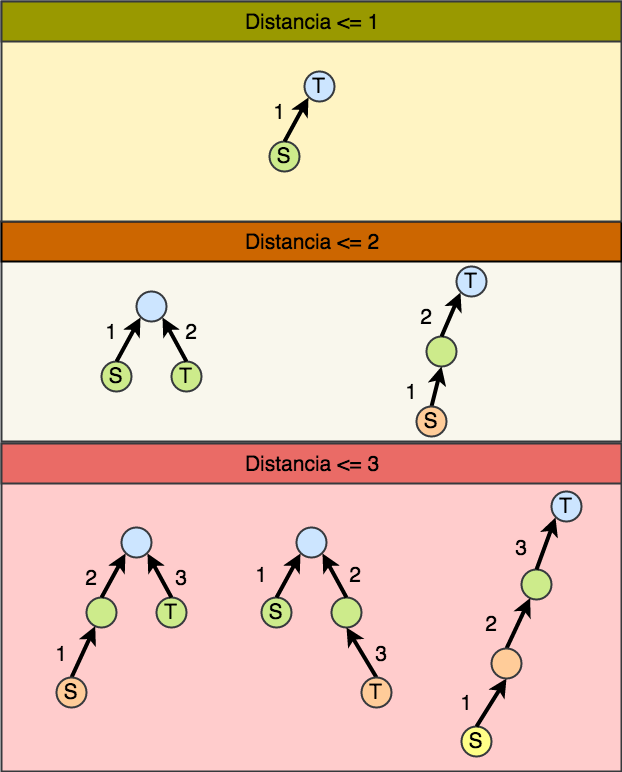
\includegraphics[width=0.5\textwidth]{distancias_semanticas}
\end{figure}

% Please add the following required packages to your document preamble:
% \usepackage{booktabs}
% \usepackage{multirow}
\begin{table}[htb]
\centering
\caption{Cubrimientos de servicios con distancias semánticas entre 1 y 3}
\label{cubrimiento_1y3}
\resizebox{\textwidth}{!}{%
\begin{tabular}{@{}lrrrrrrrr@{}}
\toprule
\multirow{2}{*}{Servicio} & \multicolumn{2}{l}{\begin{tabular}[c]{@{}l@{}}Cubrimientos con \\ Distancia Semántica \textless=3\end{tabular}} & \multicolumn{2}{l}{\begin{tabular}[c]{@{}l@{}}Cubrimientos con \\ Distancia Semántica \textless=2\end{tabular}} & \multicolumn{2}{l}{\begin{tabular}[c]{@{}l@{}}Cubrimientos con \\ Distancia Semántica \textless=1\end{tabular}} & \multicolumn{2}{l}{Cubrimientos exactos} \\ \cmidrule(l){2-9} 
 & Kaiser/Hiba & Hiba/Kaiser & Kaiser/Hiba & Hiba/Kaiser & Kaiser/Hiba & Hiba/Kaiser & Kaiser/Hiba & Hiba/Kaiser \\ \cmidrule(r){1-9}
Cardio & 0,475 & 0,947 & 0,320 & 0,890 & 0,211 & 0,782 & 0,104 & 0,457 \\
Oftalmo & 0,779 & 0,969 & 0,647 & 0,949 & 0,505 & 0,787 & 0,257 & 0,407 \\
Derma & 0,831 & 0,974 & 0,683 & 0,942 & 0,452 & 0,824 & 0,242 & 0,449 \\
Pedia & 0,85 & 0,973 & 0,769 & 0,940 & 0,594 & 0,857 & 0,305 & 0,560 \\
ENU & 0,492 & 0,979 & 0,319 & 0,944 & 0,174 & 0,811 & 0,075 & 0,403 \\
Onco & 0,582 & 0,879 & 0,433 & 0,623 & 0,307 & 0,252 & 0,073 & 0,173 \\
Psiqui & 0,572 & 0,904 & 0,476 & 0,813 & 0,384 & 0,627 & 0,227 & 0,303 \\
Orto & 0,726 & 0,986 & 0,586 & 0,963 & 0,402 & 0,860 & 0,179 & 0,420 \\
Neuro & 0,563 & 0,975 & 0,385 & 0,963 & 0,227 & 0,825 & 0,112 & 0,404 \\
Gineco & 0,597 & 0,936 & 0,443 & 0,904 & 0,284 & 0,743 & 0,119 & 0,326 \\ \bottomrule
\end{tabular}%
}
\end{table}

Como se muestra en la tabla \ref{cubrimiento_1y3}, hay una significativa mejora en los valores de cubrimiento, incluso con distancia \textless=2 todos alcanzan más de un 90\% de cubrimiento de conceptos del Kaiser por el HIBA, con excepción de Oncología. Esta mejora se explica porque el crecimiento del HIBA agrega hasta un nivel más de precisión, muchos conceptos son descendientes del mismo ancestro y al no ser tenido en cuenta porque no hay un \textit{match} exacto se descartan también todas esas ramas que crecen a lo ancho.

En el caso del cubrimiento de los conceptos de HIBA por el Kaiser, el cubrimiento también mejora pero sigue siendo muy pequeño, esto se debe a que el HIBA tiene no sólo más conceptos en los \textit{refsets} sino que se evidencia una mayor diversidad en ellos.
 
Por último, en la fase de implementación eliminé las que entraron en el criterio de exclusión y reemplacé las áreas jerárquicas con 29 servicios de atención de Snomed CT.


\subsubsection{Contexto: Nivel de asistencia}
Con el fin de encontrar conceptos que estén asociados a los niveles de asistencia apliqué los algoritmos agrupamiento \textit{leading vector}, \textit{label propagation} y \textit{multilevel}. Los valores de modularidad y número de grupos son similares en aplicando todos los algoritmos:
\begin{itemize}
\item \textit{Leading vector}, modularidad = \num{0.346} y número de grupos = 4
\item \textit{Label propagation}, modularidad = \num{0.393} y número de grupos = 5
\item \textit{Multilevel}, modularidad = \num{0.397} y número de grupos = 5
\end{itemize}

Según la tabla \ref{nivel_asistencia} se puede observar que en 4 niveles de asistencia (Ambulatorio, Guardia, Triage e Internación general) están el 97\% del total de los registros de la lista de problemas. De estos 4 niveles de asistencia, en el caso de Ambulatoria y Guardia hay una relación en la que por cada 10 registros hay 1 concepto de Snomed CT diferente asociado a la lista de problemas, Triage es la relación más baja ya que es 20:1 entre los registros y los conceptos de Snomed  CT, e Internación General es la más alta (10:2). Al aplicar los algoritmos de agrupamiento, se fusionaron los niveles de asistencia Internación general e Internación domiciliaria, con 3002 conceptos que representan su contexto, y se descarta el nivel de asistencia Episodio externo.

\begin{table}[htb]
\centering
\caption{Distribución de registros y conceptos por nivel de asistencia o ámbito }
\label{nivel_asistencia}
\begin{tabular}{@{}lrrr@{}}
\toprule
Nivel de Asistencia o ámbito & Registros & Diferentes Conceptos& Conceptos del grupo \\ \midrule
Ambulatorio & \num{771096} & \num{9543}& \num{6304} \\
Guardia & \num{603412} & \num{5759}& \num{2269} \\
Triage & \num{556166} & \num{2963}& \num{779} \\
Internación general & \num{267303} & \num{6322}& \num{3002} \\
Internación domiciliaria & \num{22297} & \num{1975} & \num{3002}\\
Episodio ambulatorio & \num{17947} & \num{1247}& \num{370} \\
Seguimiento domiciliario & \num{14537} & \num{1302} & \num{681}\\
Internación geriátrica & \num{204} & \num{115}& \num{101} \\
Episodio externo & \num{4} & \num{2} & \num{0}\\ \bottomrule
\end{tabular}
\end{table}


\subsubsection{Contexto: Grupo etario}
La distribución de los problemas registrados por edad en la figura \ref{fig:listaEdad} evidencia que los grupos etarios en los que más se consulta son 0-4 años, 25-34 años y mayores de 75 años.

Al aplicar los algoritmos de agrupamiento, obtengo resultados similares entre \textit{Leading vector} y \textit{multilevel}. \textit{Leading Vector} dividió el grafo en 5 grupos y obtuvo una modularidad de \num{0.171}, \textit{multilevel} dividió el grafo en 4 grupos y obtuvo una modularidad de \num{0.138}. En el caso del algoritmo \textit{label propagation} el valor de la modularidad es de 0, por lo tanto sus resultados son descartados.

Después de combinar los resultados de los algoritmos \textit{Leading vector} y \textit{multilevel}, para identificar los grupos que invariantemente se repitan en ambos resultados, se descarta el grupo etario de 5 a 14 años y fusionan los grupos etarios de 0 a 4, 15 a 24, 25 a 34 y 35 a 44 años. La tabla \ref{grupo_etario} contiene los tamaños finales de los grupos.

\begin{figure}[ht]
\caption{Distribución de todos los problema por edad de los pacientes}
\label{fig:listaEdad}
\centering
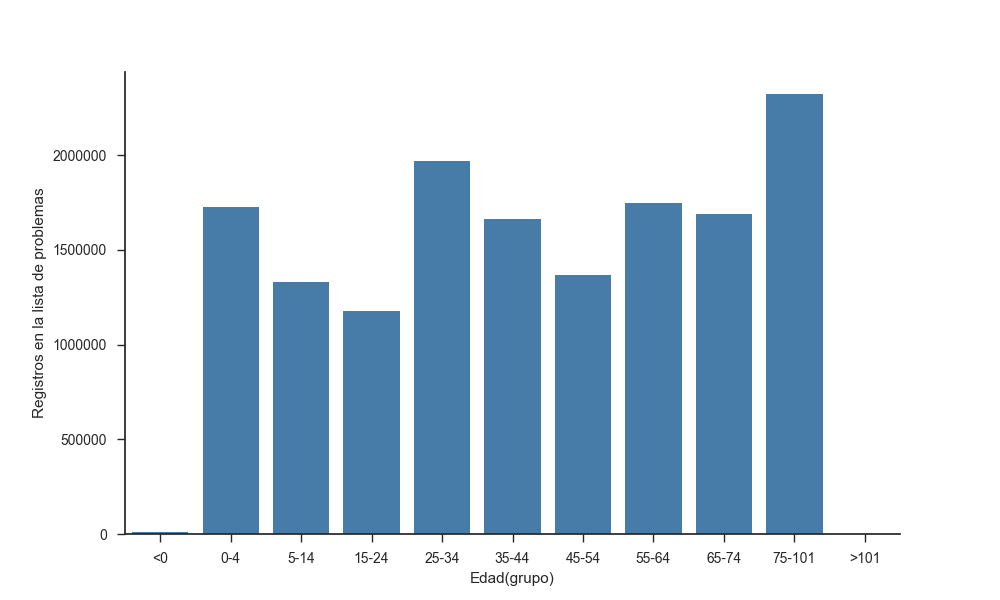
\includegraphics[width=\textwidth]{chart4}
\end{figure}

% Please add the following required packages to your document preamble:
% \usepackage{booktabs}
\begin{table}[htb]
\centering
\caption{Distribución de conceptos por grupo etario }
\label{grupo_etario}
\begin{tabular}{@{}lrr@{}}
\toprule
Grupo Etario & Diferentes Conceptos & Conceptos del grupo \\ \midrule
0-4 & \num{15264} & \num{12532} \\
5-14 & \num{24837} & \num{0} \\
15-24 & \num{29548} & \num{12532} \\
25-34 & \num{35419} & \num{12532} \\
35-44 & \num{33165} & \num{12532} \\
45-54 & \num{32644} & \num{6731} \\
55-64 & \num{35733} & \num{5073} \\
65-74 & \num{35772} & \num{5165} \\
75-101 & \num{37625} & \num{4292} \\ \bottomrule
\end{tabular}
\end{table}

\section{Discusión}
El objetivo de este capítulo era el análisis descriptivo de los datos y de los procesos de limpieza que apliqué para obtener un conjunto de datos consistente con el que realizar los experimentos de graphmining en el siguiente capítulo.

En la primera sección abordé la comprensión de los datos de la lista de problemas. Este análisis me permitió identificar outliers y datos de error al momento de la carga, revisando la distribución desde diferentes dimensiones: tiempo, individuos, conceptos y contextos: 

(a) en el caso del tiempo sólo son válidos los registros con fecha de carga desde el año 1998 hasta el tiempo presente, dado que este ha sido el lapso en el que ha estado activa la HCE; 

(b) desde el punto de vista de los individuos  el 34.1\% tiene sólo un problema, estos registros también se descartan porque carecen de co-ocurrencia con otros problemas; 

(c) en la dimensión de los conceptos, el 20\% de los registros pertenecen a 12 conceptos y sus variantes lexicográficas, estos problemas tendrán poca capacidad predictiva dado que se relacionarán con un número grande de conceptos. El uso de los conceptos presenta una distribución de cola larga, esto es consistente por lo reportado por Fung et. al.\cite{Fung2015AnCT} donde haciendo una comparación del uso de la lista de problemas de ocho instituciones, encontró que el 95\% del uso corresponde a sólo el 22.8\% de términos únicos;

(d) Los contextos analizados fueron el área jerárquica, nivel de asistencia y grupo etario, cada uno de estos contextos tiene sus particularidades.

El HIBA tiene 601 áreas jerárquicas con diferentes niveles de agregación, algunas de esas áreas corresponden a funciones administrativas. El experimento 1 permitió excluir las áreas administrativas y mapear las restantes a  44 servicios de SNOMED CT, facilitando así la interoperabilidad con otros centros médicos. 

El experimento 2 mostró que algunos de los servicios se solapan entre sí, ya que significativamente un clasificador no puede diferenciar cuándo los conceptos pertenecen a un servicio u otro, entre los servicios con F1 score más bajos tengo: servicio de anestesia (0,048), servicio audiológico (0,000), servicio de colposcopia (0,000), servicio de internación domiciliaria (0,131), servicio de patología (0,000) y servicio de psicología (0,000). Estos servicios fueron fusionados con los que más presentaban solapamiento en la matriz de confusión.

Los servicios con mejor F1 score son: servicio de cardiología pediátrica (0,871), servicio de fisioterapia (0,993), servicio de ginecoobstetricia (0,877), servicio de oftalmología adultos (0,938), servicio de psiquiatría (0,827), servicio de psiquiatria pediatrica(0,945) y  servicio de traumatología (0,821). Estos valores muestran que los conceptos diferencian bien estos servicios, y que no deberían ser fusionados aunque uno sea padre del otro como el caso de  servicio de psiquiatría y servicio de psiquiatria pediatrica.

Como resultado de esos experimentos obtuve 29 servicios finales, para evaluar el cubrimiento de los \textit{refsets}, use como referencia los donados por Kaiser Permanente a Snomed CT, en ellos encontré 10 \textit{refsets} de Kaiser Permanente que eran afines a 16 de los 29 servicios finales. Los resultados obtenidos muestran que la mayoría de los servicios tienen una cobertura entre 0,30 y 0,45, los que se ubican con mejor cobertura son pediatría (0,56), cardiología(0,46) y dermatología (0,45); y el de peor cobertura es oncología (0,07), este es el único caso en el que el \textit{refset} creado por el HIBA es de menor tamaño al de referencia, en todos los otros casos el tamaño de los \textit{refsets} del HIBA es superior en tamaño a los de referencia. 

Los niveles de precisión entre los dos conjuntos de datos hace compleja la tarea de comparación, cuando cuento los conceptos que se encuentran en el \textit{refset} de referencia, no sólo debo de tener en cuenta los mapeos directos o las relaciones is\_a exactas, porque pierdo a los conceptos que tienen mayor precisión. Por lo tanto, contrasté estos resultados con la cobertura calculada con diferentes distancias semánticas, encontrando que hay una significativa mejora en los valores de cubrimiento, incluso con distancia \textless= 2 la mayoría de los servicios alcanzan más de un 90\% de cubrimiento de conceptos del Kaiser.

Un trabajo similar reportado por Nova Scotia\cite{nova}, en el que desarrollan sus propios \textit{refsets} de especialidades, obtiene coberturas inferiores a las reportadas en esta tesis, incluso sin el cálculo de distancias semánticas (ver tabla \ref{coverage_scotia}). 

\begin{table}
 \caption{Comparación de la cobertura de las especialidades del HIBA vs Nova Scotia }
  \label{coverage_scotia}
  \resizebox{\textwidth}{!}{%
  \begin{tabular}{lcccccc} \hline
 \small
& \multicolumn{3} {c}{ Nova Scotia} & \multicolumn{3} {c}{HIBA} \\ \hline
Servicio& \# Refset & \# Kaiser & Cobertura &\# Refset & \# Kaiser  & Cobertura  \\ \hline
Cardiología&886&653 &0,18&9182&880  &0,46 \\
Dermatoloía&638&691    &0,16&11622&2757     &0,45 \\
Hematología*&714&330   &0,13&721&4086    &0,17\\
Enfermedades infecciosas&2,202&1101   &0,08&-&-&  \\
Oftamología&1,327&413&    0,34&4188&3285     &0.41\\
Cirugía ortopédica&1,306&167&   0,10&22555&1089    &0,25\\
Otoloaringología&1,344&641    &0,29&-&-&  \\
Pediatría&3,699&2181    &0,34&17325&3793     &0,56\\
Medicina respiratoria&114&511   &0,08&-&-&\\\hline

\end{tabular}
 %
}
\end{table}

En el nivel de asistencia hay desbalanceo entre los grupos. Los grupos más grandes son el nivel de asistencia ambulatorio (6304 conceptos), las internaciones que se fusionaron en una sola (3002), y la guardia (2269). Aunque el nivel de asistencia de Triage sea el tercero en cantidad de registros, el número de conceptos en su grupo es muy pequeño, lo que indica la baja diversidad de conceptos seleccionados en este nivel de asistencia. 

Los grupos etarios que más registran problemas son entre los 0-4 años, 25 y 34 años y mayores de 75 años, los registros con edades menores a 0 o mayores a 101 fueron descartadas por interpretarse como errores del sistema o casos de prueba. Utilizando los algoritmos de agrupación se fusionaron los grupos etarios entre los 0 y 44 años. Según estos algoritmos, los problemas que existen en estos grupos no tienen diferencias significativas. Al mismo tiempo, descarté el grupo etario entre 5 y 14 años, ya que los problemas no se agruparon en un grupo consistente.

\section{Conclusión}
En este capítulo he presentado las decisiones en la extracción, transformación y limpieza de la lista de problemas, para definir el conjunto de datos que será utilizado en los experimentos de graphmining. 

La transformación más compleja fue la de la definición del contexto de los 29 servicios de atención a partir de las 901 áreas jerárquicas. Si bien agrupar los conceptos por contexto es necesario para facilitar el uso significativo de la SNOMED CT, son escasos los ejemplos sobre metodologías o \textit{refsets} públicos que puedan ser usados como referencia.

En este capítulo usé técnicas de agrupamiento y aprendizaje supervisado para definir qué servicios, niveles asistenciales y grupos etarios pueden ser diferenciables de los demás a partir de sus conceptos. En el caso de los servicios, Una vez fueron definidos evalué su cubrimiento con respecto a los \textit{refsets} de referencia de kaiser permanente, aunque en la mayoría de los casos da un cubrimiento exacto superior al 40\%, si se utilizan las distancias semánticas estos cubrimientos se incrementan significativamente.

Con respecto a las distancias semánticas, este trabajo no tiene en cuenta el nivel de granularidad de los conceptos que se están comparando, por lo tanto un par de conceptos que estén muy arriba en la jerarquía y sean muy generales tienen igual distancia que dos conceptos que estén muy abajo y sean muy específicos. Sin embargo, en la práctica entre más precisos sean los conceptos que tienen similitud, se puede confiar más en que realmente tienen un significado similar.


%%%% Capítulo 4: Graphmining
%%\chapter{Minando la lista de problemas}
%%\section{Introducción}
En los capítulos anteriores realicé una revisión del estado del arte sobre el \textit{graph mining} aplicado en el área de la salud, con las definiciones en las cuales se enmarca esta tesis. Además, describí el proceso de ETL para obtener el conjunto de datos que constituye el grafo de la lista de problemas con sus relaciones a SNOMED CT, el cual es un grafo dirigido acíclico.

En éste capítulo realizaré experimentos sobre el grafo, dividiéndolo en dos versiones, la primera con las relaciones a SNOMED CT, y la segunda sin las relaciones. En capítulos anteriores se mostró inconsistencias entre los conceptos de la red de SNOMED CT, donde conceptos muy similares estaban muy distantes y conceptos muy distintos estaban muy cerca, es de interés analizar si las conexiones de SNOMED mejoran la capacidad de formar comunidades y la capacidad predictiva de los modelos.

En la primera parte de este capítulo aplicaré las definiciones de los grafos descriptas en los capítulos anteriores, evaluando si los grafos formados siguen patrones de red. 

La segunda parte contiene el análisis sobre los agrupamientos encontrados luego de aplicar los algoritmos \textit{label propagation}, \textit{leading vector} y \textit{multilevel}. Las red creada sólo a partir de los problemas y sus conexiones será enriquecida con información sobre el nivel asistencial, grupo etáreo y servicio de salud en el cuál el problema fue seleccionado. 

Además de describir los resultados obtenidos y los outliers encontrados, se evaluará la capacidad predictiva de los conceptos que están en el mismo grupo dada una lista de problema de un paciente.

\section{Definición del grafo}
Sea el grafo de la figura\ref{fig:ModeloGrafo} G=(V,E), donde V denota a los vértices, equivalente a nodos: conceptos de snomed CT y pacientes, y E denota las aristas, equivalente a relaciones: \textit{tiene un problema}, o conexiones jerárquicas $|\textit{is a}|$ (Hallazgo Clínico, Procedimientos, Eventos, Situación con contexto explícito). Los \num{88869} conceptos distintos de la lista de problemas están relacionados jerárquicamente con \num{11946} de snomed, de tal manera que al usar todos los conceptos de las jerarquías, el número de vértices y aristas de la red son $|V|=$\num{19354} y $|E|=$\num{1173234} respectivamente. Las aristas de la red son ponderadas por la frecuencia de ocurrencia del problema en el paciente. 

De manera paralela, realizo el análisis sobre el subgrafo generado sólo con las relaciones \textit{tiene un problema} y los nodos que comparten esta relación. El número de vértices y aristas de este subgrafo son $|V|=$\num{11946} y $|E|=$\num{937107} respectivamente.

Para diferenciar las dos redes, la primera la nombro como \textbf{Red semántica de problemas(RSP)} y la segunda la nombro como \textbf{Red de problemas(RP)}

\begin{figure}[ht]
\caption{Modelo de datos de grafos de la lista de problemas}
\label{fig:ModeloGrafo}
\centering
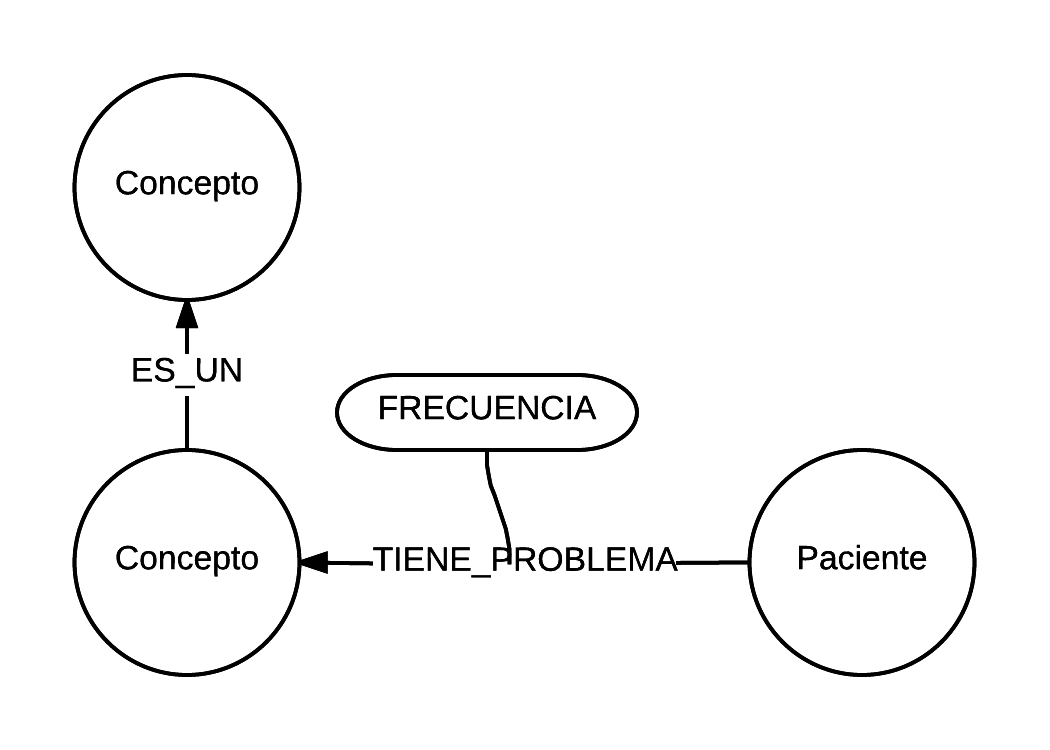
\includegraphics[width=0.6\textwidth]{Modelo_grafo_}
\end{figure}

\section{Patrones de la red de la lista de problemas}
\subsubsection{Red libre de escala}
En esta sección evalúo si la redes comparte patrones con redes de gran escala, realizo un ajuste a una distribución de ley de potencias usando los grados de cada nodo, con la $H0:$ los datos se distribuyen según la ley de potencias, y estimo la función de distribución acumulativa (cdf). Si el p-value no permite rechazar la hipótesis nula otra estrategia para determinar la distribución de los datos es comparar el estadístico \textit{log-likelihood ratio} con otras dos distribuciones, el resultado es positivo si los datos se ajustan más a la primera distribución, y negativa si los datos son más como la segunda distribución.

En el caso de la \textbf{RSP} la función cdf es:
\begin{equation}
F(X\geq 51) \propto x^{-1.82 +1}
\end{equation}

Dado que el p-value$(0.3188>0.05)$ no me permite rechazar la hipótesis nula, realizo la comparación con otras distribuciones. En la tabla \ref{distribucion} están los resultados de las comparaciones realizadas entre ley de potencias con otras distribuciones: la distribución exponencial fue usada para confirmar que los datos tienen una cola pesada, y la distribución lognormal tiene un mejor ajuste que la ley de potencias, como se muestra también en la figura \ref{fig:ajusteDistribuciones}.

% Please add the following required packages to your document preamble:
% \usepackage{booktabs}
\begin{table}[htb]
\centering
\caption{Comparación de la ley de potencias con otras distribuciones de la red semántica de problemas}
\label{distribucion}
\begin{threeparttable}
\begin{tabular}{@{}lr@{}}
\toprule
Distribución & Resultado    \\ \midrule
Exponencial  & 10.64\tnote{*}  \\
Lognormal    & -1.5 \\ \bottomrule
\end{tabular}
\begin{tablenotes}
    \item[*] p-value$<$\num{0.05}.
  \end{tablenotes}
\end{threeparttable}
\end{table}

\begin{figure}[ht]
\caption{Gráfico log-log, comparación de ajuste de distribuciones de la red semántica de problemas}
\label{fig:ajusteDistribuciones}
\centering
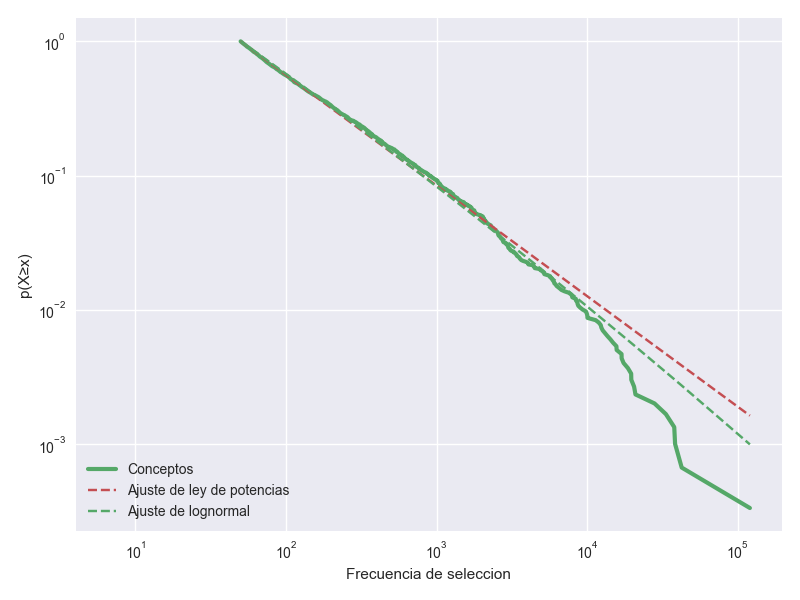
\includegraphics[width=0.6\textwidth]{chart6}
\end{figure}

En el caso de la \textbf{RP} la función cdf es:
\begin{equation}
F(X\geq 279) \propto x^{-1.86 +1}
\end{equation}

Dado que el p-value$(0.03<0.05)$ se acepta la hipótesis $H0:$ los datos se distribuyen según la ley de potencias. La figura \ref{fig:ajusteDistribucionesRP} muestra también que esta distribución tiene mejor ajuste.

\begin{figure}[ht]
\caption{Gráfico log-log, comparación de ajuste de distribuciones de la red de problemas}
\label{fig:ajusteDistribucionesRP}
\centering
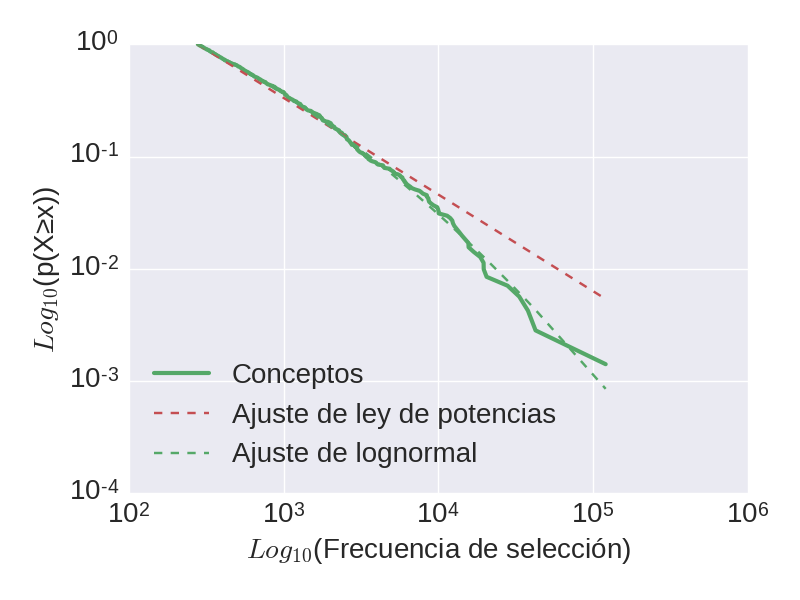
\includegraphics[width=0.6\textwidth]{chart7}
\end{figure}

% fit.distribution_compare('power_law', 'exponential', normalized_ratio = True)
%(4.6415121033253648, 3.4586875833842345e-06)
%>>> fit.distribution_compare('power_law', 'lognormal', normalized_ratio = True)(-2.4059692368632613, 0.016129622892949523)

\subsubsection{Fuertes estructuras de comunidad}
Existen diferentes métricas para evaluar cuantitativamente los efectos de comunidad en un grafo, las usadas  a continuación siguen el trabajo de Boccaletti \textit{et. al}\cite{BOCCALETTI2006} y están disponibles en los paquetes igraph\cite{igraph} y netowrkx\cite{SciPyProceedings_11} de python.

\begin{table}[htb]
\centering
\caption{Métricas de efectos de comunidad en redes}
\label{community-graphs}
\resizebox{\textwidth}{!}{%
\begin{tabular}{@{}lrr@{}}
\toprule
Métrica                                                  & Valor en la RSP  & Valor en la RP            \\ \midrule
Coeficiente de agrupamiento - transitividad                & \num{0.19} & \num{0.21} \\
Coeficiente de agrupamiento - transitividad local promedio & \num{0.41}  & \num{0.80}\\
Coeficiente de agrupamiento promedio                        & \num{0.34}  & \num{0.78}      \\
Longitud media del camino mínimo entre nodos             & \num{2.80}  & \num{2.17}  \\
Promedio de grados                                       & \num{60.62}  & \num{78.4}      \\ \bottomrule
\end{tabular}%
}
\end{table}

La diferencia de las métricas de transitividad y la transitividad local promedio, es que la primera es la medida de la transitividad local en toda la red, en la segunda se calcula por cada vértice la transitividad y los nodos con menos de dos vecinos son considerados como de transitividad cero\cite{Watts1998}. Las diferencias entre estas dos métricas indican una alta presencia de nodos que no forman tríadas.

Los valores de coeficiente de agrupamiento cercanos a 1 indican alto grado de agrupamiento, como se puede ver en la tabla \ref{community-graphs} la \textbf{RP} tiene mejores coeficientes que la \textbf{RSP}. 

Aunque los valores de la longitud media del camino mínimo entre nodos entre las dos redes es similar, para un alto coeficiente de agrupamiento como es el caso de \textbf{RP} el efecto es que la mayoría de los nodos que son homogéneos se encuentran en pocos saltos dentro de la red, este efecto es similar al fenómeno de mundo pequeño en las redes sociales\cite{Cook2006}. Además, estos nodos tienen en promedio más nodos vecinos que la \textbf{RSP}.

\section{Agrupamiento}

Apliqué los algoritmos de agrupamiento: \textit{label propagation}, \textit{leading vector} y \textit{multilevel} a el grafo de la \textbf{RP} y a sub-grafos de la \textbf{RSP}, conformados por relaciones que tengan un mínimo de frecuencia en pacientes (\num{5}, \num{10}, \num{100}, \num{1000} y \num{10000}). Esto con el propósito de evaluar la estabilidad de los agrupamientos aunque el grafo pierda nodos.

La tabla \ref{res_agru} contiene los resultados de los coeficientes de agrupamiento para cada grafo y la cantidad de grupos encontrados. Se puede observar que en el caso del grafo de la \textbf{RP} se generan similares número de grupos aunque el coeficiente de clustering varía en los algoritmos. El más alto coeficiente es el del algoritmo \textit{multilevel} y el más bajo es el de \textit{label propagation}, aunque estos dos son algoritmos aglomerativos el primero optimiza la ganancia en la función de modularidad, mientras que el segundo realiza un consenso entre los nodos de un mismo grupo para decidir el grupo al que pertenecen todos.

En el caso de los grafos \textbf{RSP}, el número de grados varía entre algoritmos, \textit{multilevel} es también el que mejores coeficientes obtiene y mientras que \textit{leading vector} va desmejorando en sus coeficientes a medida que crece el grafo, \textit{label propagation} mejora. \textit{leading vector} es un algoritmo divisivo que se ve afectado por el tamaño del grafo y \textit{label propagation} va hallando estructuras más cohesivas en la medida que crece el grafo.


% Please add the following required packages to your document preamble:
% \usepackage{booktabs}
% \usepackage{multirow}
% \usepackage{graphicx}
\begin{table}[htb]
\centering
\caption{Resultados de agrupamiento de grafos de problemas}
\label{res_agru}
\resizebox{\textwidth}{!}{%
\begin{tabular}{@{}lrrrrrr@{}}
\toprule
\multirow{3}{*}{Grafo}                                                                                          & \multicolumn{6}{l}{Algoritmos de clasifcación}                                                                                                                                             \\ \cmidrule(l){2-7} 
                                                                                                                & \multicolumn{2}{l}{Leading Vector}                           & \multicolumn{2}{l}{Multilevel}                               & \multicolumn{2}{l}{Label Propagation}                        \\ \cmidrule(l){2-7} 
                                                                                                                & \multicolumn{1}{l}{Coeficiente} & \multicolumn{1}{l}{Grupos} & \multicolumn{1}{l}{Coeficiente} & \multicolumn{1}{l}{Grupos} & \multicolumn{1}{l}{Coeficiente} & \multicolumn{1}{l}{Grupos} \\ \cmidrule(r){1-7}
Red de Problemas(RP)                                                                                                & 0.36                            & 22                         & 0.43                            & 23                         & 0.08                            & 22                         \\
\begin{tabular}[c]{@{}l@{}}Red Semántica de Problemas \\ (Relaciones en al menos 10000 individuos)\\(RSP-10.000)\end{tabular} & 0.50                            & 14                         & 0.59                            & 27                         & 0.27                            & 87                         \\
\begin{tabular}[c]{@{}l@{}}Red Semántica de Problemas \\ (Relaciones en al menos 1000 individuos)\\(RSP-1.000)\end{tabular}  & 0.50                            & 14                         & 0.59                            & 27                         & 0.27                            & 88                         \\
\begin{tabular}[c]{@{}l@{}}Red Semántica de Problemas \\ (Relaciones en al menos 100 individuos)\\(RSP-100) \end{tabular}   & 0.50                            & 14                         & 0.59                            & 24                         & 0.29                            & 92                         \\
\begin{tabular}[c]{@{}l@{}}Red Semántica de Problemas \\ (Relaciones en al menos 10 individuos)\\(RSP-10) \end{tabular}    & 0.29                            & 11                         & 0.61                            & 24                         & 0.37                            & 91                         \\
\begin{tabular}[c]{@{}l@{}}Red Semántica de Problemas \\ (Relaciones en al menos 5 individuos)\\(RSP-5)\end{tabular}     & 0.32                            & 12                         & 0.62                            & 25                         & 0.46                            & 88                         \\ \bottomrule
\end{tabular}%
}
\end{table}

Estos seis grafos con sus 3 algoritmos representan grupos fuertes y débiles, a continuación presento los grupos de problemas que son consistentes en todos los agrupamientos. Además calculo la longitud media del camino mínimo entre los nodos del agrupamiento, medida que es usada como distancia semántica en diferentes trabajos en el dominio médico\cite{Wang2010TheAudit.,Gan2013,Pedersen2007,Zare2015ASNOMED-CT}. Esta información permite detectar grupos con conceptos con diferentes significados semánticos y outliers.

\subsection{Agrupamientos de Red de Problemas (RP)}
Combinando los resultados de los agrupamientos hay \num{11132} posibles combinaciones, encontré 53 grupos de problemas que comparten las mismas agrupaciones. Según la tabla, \ref{gruposRP} la mayoría (19) de los grupos encontrados tienen 2 nodos, los grupos que tiene más nodos tienen en promedio una mediana de grados por nodo más grande, es decir que son nodos altamente conectados.

Al analizar las distancias semánticas entre los conceptos que comparten el mismo grupo, puedo observar según la figura \ref{fig:bpDistanciasSemanticasRP} que la mayoría de las medianas de las distancias se ubican cercanas a 10. Los casos con las mayores dispersiones son el cluster\_1, cluster\_6, cluster\_10, cluster\_16, cluster\_22, cluster\_27, cluster\_30, cluster\_34 y cluster\_36. 

En la tabla \ref{top10_rp} se encuentra el top 10 de los conceptos por agrupamiento según diferentes métricas de centralidad (grado, cercanía e intermediación). En esta tabla se encuentran sólo los casos de las mayores dispersiones, el top 10 según el grado y la cercanía es muy similar en la mayoría de los casos; difiere en el caso de la intermediación, donde se pueden encontrar nodos que sin tener muchas conexiones son mucho más importantes para la conexión de otros dos nodos.

Por ejemplo, según lo anterior en el caso del cluster\_6 (que se puede interpretar como de enfermedades generales), los problemas con mayor grado (los más populares) son: FIEBRE y TOS, pero el problema con mayor intermediación es RESFRIÓ COMÚN. Es decir, que este último conecta más otros pares de problemas que la Fiebre y la Tos. Otros ejemplos se pueden encontrar en el cluster\_10, donde el problema con mayor grado y cercanía es MALESTAR GENERAL, y el de mayor intermediación es INMUNODEFICIENCIA COMBINADA SEVERA; en el grupo de embarazo (cluster\_16) donde los problemas con mayor grado son PACIENTE ACTUALMENTE EMBARAZADA, ANSIEDAD y MAREO, pero los de mayor intermediación son AMENAZA DE TRABAJO DE PARTO PREMATURO, INTOXICACIÓN POR FÁRMACO Y/O SUSTANCIA MEDICINAL y SANGRADO VAGINAL.

\subsubsection{outliers}
Según el boxplot generado con las distancias semánticas en la figura \ref{fig:bpDistanciasSemanticasRP}, se presentan outliers en los siguientes clusters:
\begin{itemize}
\item cluster\_6: Este es un agrupamiento de enfermedades generales donde los problemas que tiene mayor distancia semántica en promedio con el resto del mismo grupo es: CIRUGÍA DE CATARATAS(PROCEDIMIENTO), ATAQUE DE PÁNICO(HALLAZGO), AMIGDALECTOMÍA(PROCEDIMIENTO)
\item cluster\_10: Este es un agrupamiento de administración de medicamentos y procedimientos invasivos, los problemas con mayores distancias son: ADMINISTRACIÓN DE ANTICOAGULANTE(PROCEDIMIENTO), TRATAMIENTO CON ANTIBIÓTICOS INTRAVENOSOS(PROCEDIMIENTO), INYECCIÓN DE GAMMAGLOBULINA (PROCEDIMIENTO), CAMBIO DEL TUBO DE TRAQUEOSTOMÍA (PROCEDIMIENTO). Estas distancias se explican porque la mayoría de los conceptos de este grupo están en la jerarquía de Hallazgos.
\item cluster\_27: En este agrupamiento de enfermedades relacionadas con la edad avanzada, los problemas que tienen mayor distancia son: CONFUSIÓN AGUDA(HALLAZGO), PACIENTE EN CAMA (HALLAZGO).
\item cluster\_36: En este agrupamiento de enfermedades cardiopulmonares, las mayores distancias se encuentran en los siguientes conceptos: BIOPSIA ENDOMIOCÁRDICA (PROCEDIMIENTO), ALOTRASPLANTE ORTOTÓPICO DE CORAZÓN (PROCEDIMIENTO) y TUMOR DE KLATSKIN (TRASTORNO), esta última considerada como una enfermedad huérfana\footnote{www.orpha.net/consor/cgi-bin/OC\_Exp.php?lng=ES\&Expert=99978}.
\end{itemize}

Los outliers en las cotas inferiores se debe a relaciones de especificación entre conceptos, por ejemplo: en el cluster\_42: EPISTAXIS ANTERIOR es descendiente de EPISTAXIS, y ambos conceptos están en el mismo grupo.

% Please add the following required packages to your document preamble:
% \usepackage{booktabs}
\begin{table}[htb]
\centering
\caption{Grupos que comparten las mismas agrupaciones en la red de problemas}
\label{gruposRP}
\begin{tabular}{@{}rrr@{}}
\toprule
Número de Nodos & Grupos Encontrados & Mediana de grados por nodo \\ \midrule
2               & 19                 & 1949                       \\
3               & 9                  & 1832                       \\
4               & 5                  & 1833                       \\
5               & 1                  & 1818                       \\
6               & 5                  & 3287                       \\
7               & 1                  & 1590                       \\
8               & 2                  & 5192                       \\
10              & 2                  & 2222                       \\
13              & 1                  & 802                        \\
16              & 1                  & 990                        \\
22              & 1                  & 2198                       \\
25              & 1                  & 3008                       \\
34              & 1                  & 4210                       \\
45              & 1                  & 864                        \\
59              & 1                  & 3700                       \\
77              & 1                  & 1228                       \\
84              & 1                  & 3234                       \\ \bottomrule
\end{tabular}
\end{table}

\begin{figure}[ht]
\caption{Distancias semánticas entre conceptos del cluster}
\label{fig:bpDistanciasSemanticasRP}
\centering
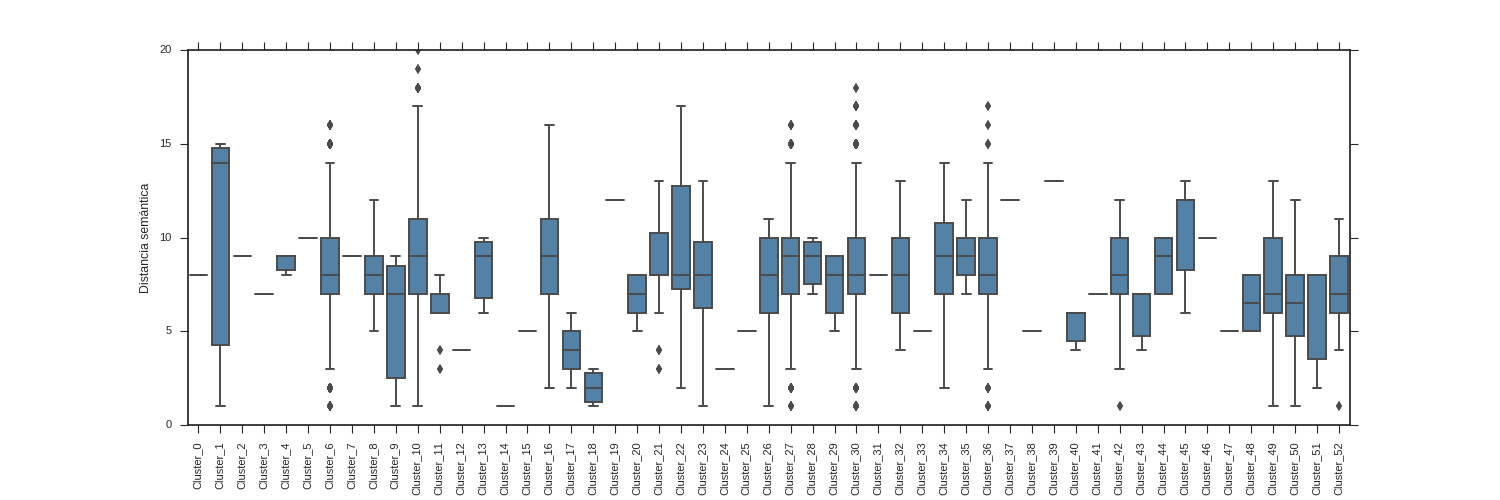
\includegraphics[width=\textwidth]{bpDistanciasSemanticasRP}
\end{figure}

\subsection{Agrupamientos de Red Semántica de Problemas (RSP)}
Combinando los resultados de los agrupamientos hay \num{2,39e26} posibles combinaciones, encontré 68 grupos de problemas que comparten las mismas agrupaciones. Según la tabla \ref{gruposRSP} La mayoría (44) de los grupos encontrados tienen 2 nodos.

Al analizar las distancias semánticas entre los conceptos que comparten el mismo grupo, puedo observar según la figura \ref{fig:bpDistanciasSemanticasRSP} que las medianas de las distancias tienen un mínimo de 1 y máximo de 10, y no presentan una tendencia. 

En la tabla \ref{top10_rsp} se encuentra el top 10 de los conceptos por agrupamiento según diferentes métricas de centralidad (grado, cercanía e intermediación). Estos grupos son más pequeños que el caso anterior, pero sobresalen los grupos con distancias semánticas grandes cuyos conceptos pareciera que no están muy relacionados, por ejemplo, el cluster\_0: INCISIÓN DE LA TRÁQUEA, AMIGDALECTOMÍA y CIRUGÍA DE CATARATAS, el cluster\_2: FÍSTULA TRAQUEOESOFÁGICA y ÚTERO UNICORNE, el cluster\_6: HIPERCORTISOLISMO y TUMOR DE KLATSKIN, pero al hacer una búsqueda rápida se pueden encontrar evidencias de las relaciones de estas enfermedades en artículos de divulgación científica, como se muestra en la tabla \ref{evidencia_grupos_2}.

\subsubsection{outliers}
Según el boxplot generado con las distancias semánticas en la figura \ref{fig:bpDistanciasSemanticasRSP}, se presentan outliers sólo en el cluster\_56 formado por: PROCTORRAGIA, INDIGESTIÓN, DISFAGIA, VEJIGA: INCONTINENTE, CÁLCULO RENAL, HEMORRAGIA DIGESTIVA BAJA, SÍNDROME DE ICTERICIA COLESTÍSICA y PIELONEFRITIS. Los problemas con mayores distancias son VEJIGA: INCONTINENTE y SÍNDROME DE ICTERICIA COLESTÍSICA


% Please add the following required packages to your document preamble:
% \usepackage{booktabs}
\begin{table}[htb]
\centering
\caption{Grupos que comparten las mismas agrupaciones en la red semántica de problemas}
\label{gruposRSP}
\begin{tabular}{@{}rrr@{}}
\toprule
Número de Nodos & Grupos Encontrados & Mediana de grados por nodo \\ \midrule
2	& 44	&2041 \\
3	&12 &	2144\\
4	&3&	1843\\
5	&4&	1826\\
6	&2&	1226\\
8	&2&	3501\\
9	&1&	1172                   \\ \bottomrule
\end{tabular}
\end{table}

\begin{figure}[ht]
\caption{Distancias semánticas entre conceptos del cluster}
\label{fig:bpDistanciasSemanticasRSP}
\centering
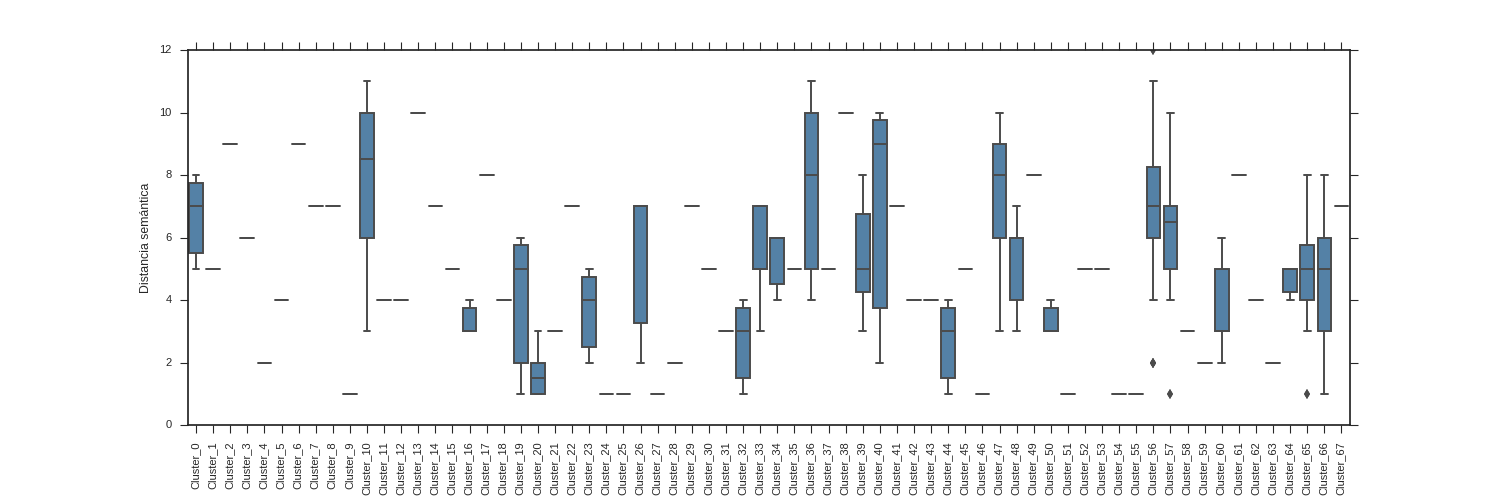
\includegraphics[width=\textwidth]{bpDistanciasSemanticasRSP}
\end{figure}

\subsubsection{Agrupamientos \textit{Label Propagation}}
Combinando los resultados de aplicar el algoritmo \textit{label propagation} en la RSP con diferentes cantidades mínimas de individuos que tengan el problema, hay \num{5.64e9} posibles combinaciones y encontré 232 grupos comunes a todos los resultados de agrupamiento. 

Según los resultados obtenidos, resumidos en la tabla \ref{clus_lp}, más del 50\% de los grupos tienen menos de 50 nodos, estos grupos son muy cohesivos, ya que tienen distancias en promedio de dos saltos entre nodos y con una baja cantidad total de distancias outliers entre los nodos (10 en total en 144 grupos). Los grupos más grandes tienen también la mayor cantidad de distancias outliers, se presentó el caso de los clusters 18 y 215 con \num{15083524} y \num{894907} número de distancias entre nodos respectivamente, y entre los dos suman más de \num{6600} distancias outliers.

% Please add the following required packages to your document preamble:
% \usepackage{booktabs}
% \usepackage{graphicx}
\begin{table}[htb]
\centering
\caption{Agrupamientos con el algoritmo \textit{Label propagation}}
\label{clus_lp}
\resizebox{\textwidth}{!}{%
\begin{tabular}{@{}lrrrrrr@{}}
\toprule
Número de nodos & \multicolumn{1}{l}{\begin{tabular}[c]{@{}l@{}}Número de \\ agrupamientos\end{tabular}} & \multicolumn{1}{l}{\begin{tabular}[c]{@{}l@{}}Promedio de mediana \\ de distancias \\ entre nodos\end{tabular}} & \multicolumn{1}{l}{\begin{tabular}[c]{@{}l@{}}Desviación estándar\\ de Mediana de distancias \\entre nodos\end{tabular}} & \multicolumn{1}{l}{\begin{tabular}[c]{@{}l@{}}Mediana  máxima \\de distancias \\entre nodos\end{tabular}}  & \multicolumn{1}{l}{\begin{tabular}[c]{@{}l@{}}Mediana mínima \\de distancias \\entre nodos\end{tabular}} & \multicolumn{1}{l}{\begin{tabular}[c]{@{}l@{}} Distancias Outliers\\ entre todos los\\ agrupamientos\end{tabular}} \\ \midrule
Menores de 50 nodos & 144 & 2 & 1,7 & 10 & 1 & 10 \\
Entre 50 y 100 nodos & 25 & 2 & 0,8 & 5 & 2 & 34 \\
Entre 100 y 200 nodos & 13 & 3 & 1,4 & 8 & 2 & 0 \\
Entre 200 y 500 nodos & 20 & 3 & 1,1 & 7 & 2 & 56 \\
Entre 500 y 1000 nodos & 10 & 4 & 1,4 & 7 & 3 & 106 \\ 
Mayor de 1000 nodos & 20 & 6 & 1,4 & 9 & 4 & 6600 \\\bottomrule
\end{tabular}%
}
\end{table}

\subsubsection{Agrupamientos \textit{Leading vector}}
Combinando los resultados de aplicar el algoritmo \textit{Leading Vector} en la RSP con diferentes cantidades mínimas de individuos, hay \num{3.62e5} posibles combinaciones y encontré 38 grupos comunes a todos los resultados de agrupamiento.

Según la tabla \ref{clus_lv}, el 50\% de los agrupamientos tienen más de 1000 nodos. El resto de los grupos son bastante cohesivos, con distancias promedios cercanas a 3 y sin distancias outliers.

\begin{table}[htb]
\centering
\caption{Agrupamientos con el algoritmo \textit{Leading vector}}
\label{clus_lv}
\resizebox{\textwidth}{!}{%
\begin{tabular}{@{}lrrrrrr@{}}
\toprule
Número de nodos & \multicolumn{1}{l}{\begin{tabular}[c]{@{}l@{}}Número de \\ agrupamientos\end{tabular}} & \multicolumn{1}{l}{\begin{tabular}[c]{@{}l@{}}Promedio de mediana \\ de distancias \\ entre nodos\end{tabular}} & \multicolumn{1}{l}{\begin{tabular}[c]{@{}l@{}}Desviación estándar\\ de Mediana de distancias \\entre nodos\end{tabular}} & \multicolumn{1}{l}{\begin{tabular}[c]{@{}l@{}}Mediana  máxima \\de distancias \\entre nodos\end{tabular}}  & \multicolumn{1}{l}{\begin{tabular}[c]{@{}l@{}}Mediana mínima \\de distancias \\entre nodos\end{tabular}} & \multicolumn{1}{l}{\begin{tabular}[c]{@{}l@{}}Distancias Outliers\\ entre todos los\\ agrupamientos\end{tabular}} \\ \midrule
Menores de 50 nodos & 15 & 3,4 & 2,8 & 9 & 1 & 0 \\
Entre 50 y 100 nodos & 3 & 3 & 1,7 & 5 & 2 & 0 \\
Entre 100 y 200 nodos & 1 & 3 & - & 3 & 3 & 0 \\
Entre 500 y 1000 nodos & 2 & 5,5 & 0,7 & 6 & 5 & 0 \\
Mayor de 1000 nodos & 19 & 7 & 1,2 & 9 & 5 & 50712 
\\\bottomrule
\end{tabular}%
}
\end{table}

\subsubsection{Agrupamientos \textit{Multilevel}}
Combinando los resultados de aplicar el algoritmo \textit{Multilevel} en la RSP con diferentes cantidades mínimas de individuos, hay \num{1.05e7} posibles combinaciones y encontré 199 grupos comunes a todos los resultados de agrupamiento.

Según la tabla \ref{clus_ml}, el 50\% de los agrupamientos tienen menos de 50 nodos, en grupos cohesivos con distancias de 3 en promedio y pocos nodos con distancias outliers.

\begin{table}[htb]
\centering
\caption{Agrupamientos con el algoritmo \textit{Multilevel}}
\label{clus_ml}
\resizebox{\textwidth}{!}{%
\begin{tabular}{@{}lrrrrrr@{}}
\toprule
Número de nodos & \multicolumn{1}{l}{\begin{tabular}[c]{@{}l@{}}Número de \\ agrupamientos\end{tabular}} & \multicolumn{1}{l}{\begin{tabular}[c]{@{}l@{}}Promedio de mediana \\ de distancias \\ entre nodos\end{tabular}} & \multicolumn{1}{l}{\begin{tabular}[c]{@{}l@{}}Desviación estándar\\ de Mediana de distancias \\entre nodos\end{tabular}} & \multicolumn{1}{l}{\begin{tabular}[c]{@{}l@{}}Mediana  máxima \\de distancias \\entre nodos\end{tabular}}  & \multicolumn{1}{l}{\begin{tabular}[c]{@{}l@{}}Mediana mínima \\de distancias \\entre nodos\end{tabular}} & \multicolumn{1}{l}{\begin{tabular}[c]{@{}l@{}}Distancias Outliers\\ entre todos los\\ agrupamientos\end{tabular}} \\ \midrule
Menores de 50 nodos & 109 & 3 & 2,2 & 9 & 1 & 4 \\
Entre 50 y 100 nodos & 21 & 4 & 1,5 & 6 & 2 & 2 \\
Entre 100 y 200 nodos & 13 & 4 & 1,8 & 8 & 2 & 50 \\
Entre 200 y 500 nodos & 15 & 4 & 1,1 & 6 & 3 & 26 \\
Entre 500 y 1000 nodos & 11 & 6 & 1,6 & 9 & 4 & 66 \\
Mayor de 1000 nodos & 31 & 6 & 1,0 & 8 & 4 & 46345 
\\\bottomrule
\end{tabular}%
}
\end{table}


\subsection{Capacidad predictiva de los agrupamientos}
Cada uno de los grupos encontrados en la sección anterior representa opciones de sugerencias para los usuarios, es decir si una lista de problemas tiene alguno de estos conceptos los otros conceptos pueden ser sugeridos al profesional de la salud para que complete la lista del paciente.

La evaluación la realicé con grupos con menos de 1000 conceptos. Teniendo en cuenta las directrices de recuperación de información, seleccioné un conjunto de pruebas que tiene tres componentes: (a) Los conceptos de snomed ct a ser recuperados; (b) Un conjunto de pruebas con los problemas que ingresaron a la lista en el 2017, estos problemas pertenecen a pacientes que previamente se le había registrado al menos un problema. Los problemas registrados previamente representan la \textit{query} y los problemas del 2017 representan la respuesta correcta; (c) una medida de relevancia por cada par de \textit{query}-concepto recuperado, esta medida es la transitividad o la distancia semántica\cite{Manning2008IntroductionRetrieval,Hersh1994OHSUMED:Research}.

La precisión y la exactitud (\textit{accuracy}) son obtenidas para evaluar la capacidad del modelo de obtener resultados relevantes. Estas medidas están definidas como:

\begin{equation}
Exactitud = \frac{\text{Verdaderos positivos}+\text{Verdaderos negativos}}{\text{Total de los datos}}
\end{equation}

\begin{equation}
Precision = \frac{\text{Documentos relevantes recuperados}}{\text{Documentos recuperados}}
\end{equation}

La exactitud suma los verdaderos positivos que son los conceptos predichos correctamente en el año 2017 y los verdaderos negativos que son los casos en los que se detecta que no hay suficiente evidencia para generar sugerencias y los divide en la totalidad de los datos de prueba (\num{156228})

La precisión toma en cuenta todos los conceptos recuperados, evalúa si existe al menos un verdadero positivo en los primeros resultados devueltos por el sistema. La medida es llamada precisión al n o P@n y exactitud al n o Acc@n.

La tabla \ref{predic_agru_c} contiene los resultados de precisión y exactitud en el top 10 de los resultados más relevantes ordenados por transitividad, en la tabla \ref{predic_agru_c_unique} no se tienen en cuenta las repeticiones. Los verdaderos positivos se cuentan en los casos de predicciones exactas, o cuando la distancia entre las predicciones y el verdadero resultado es menor o igual a 2. Los nodos excluidos sirven para filtrar los que por su alta medida de centralidad generan muchos falsos positivos, por ejemplo según el grado el concepto más popular es FIEBRE, pero al aparecer en una lista de problemas como \textit{query} hay \num{51606} posibles conceptos diferentes con los que está relacionado. Las medidas de centralidad con los que filtré y ordené los resultados son grado, intermediación, cercanía y \textit{eigenvector}. 

Se puede observar en ambas tablas, que en el caso de las predicciones exactas, los resultados con precisiones más altas se logran con 20 nodos excluidos en grados, cercanía y \textit{eigen vector}, y en el caso de intermediación aumenta en la medida que más se filtren datos, con un máximo local en 400 nodos. Esto es por la relación entre falsos positivos y verdaderos positivos que se muestra en la tabla \ref{best_results_clu} y \ref{best_results_clu_unique} donde los filtros por grado, cercanía e \textit{eigen vector} tienen mejores resultados por que tienen menos falsos positivos, y en el caso de la intermediación por que tienen más verdaderos positivos.

Siguiendo con las predicciones exactas, en el caso de las mediciones sin repeticiones se observa una exactitud similar en todos los experimentos e inferior a los resultados con repeticiones y una mejora no significativa en la precisión. A diferencia de los experimentos con repeticiones donde se obtiene una exactitud máxima de \num{0,397}, en el caso de los experimentos sin repeticiones la exactitud máxima es de \num{0,255}, esto se debe a que los verdaderos negativos cuentan con muchas repeticiones, en algunos casos reduciéndose a más de la mitad el conteo.

Cuando las predicciones no son exactas, sino que se toma como verdadero positivo si al menos hay una distancia de 2 entre la respuesta y las predicciones, hay un incremento significativo de ellos (ver tabla \ref{best_results_clu} y \ref{best_results_clu_unique}). Por lo tanto, los valores de precisión y exactitud aumentan, presentándose los máximos en los casos en los que no se excluyen nodos. Estos valores son en ordenamiento por grado y cercanía P@10(\num{0,948}) y Acc@10(\num{0,949}) y ordenando por \textit{eigen vector} P@10(\num{0,947}) y Acc@10(\num{0,948}). En el caso de Intermediación, como en las predicciones exactas, el máximo local está cuando se excluyen 400 nodos, donde se obtienen P@10(\num{0,972}) y Acc@10(\num{0,973}). 

En el caso del ordenamiento por distancia semántica y predicciones exactas, las tablas \ref{predic_agru_ds} con repeticiones y \ref{predic_agru_c_unique} sin repeticiones, muestran que se tienen mejores resultados en la precisión incluso sin realizar ningún filtro por medidas de centralidad, pero en cuanto a la medida de exactitud, se obtienen mejores resultados en el ordenamiento por transitividad. Por lo tanto, la medida de transitividad permite identificar mejor los verdaderos negativos que las distancias semánticas (ver tabla \ref{best_results_clu} y \ref{best_results_clu_unique}). 

Observando en las columnas de las predicciones con distancias menores o iguales a 2 a la respuesta correcta en las tablas \ref{predic_agru_ds} y \ref{predic_agru_c_unique} que corresponden a ordenamiento por distancia semántica con y sin repeticiones, se mantiene la tendencia de las predicciones exactas y obtengo los mejores valores de precisión y exactitud, con P@10(\num{0,995}) y Acc@10(\num{0,995}) con repeticiones y P@10(\num{0,997}) y Acc@10(\num{0,723}) sin repeticiones en distancias de ordenadas de menor a mayor. La eliminación de los top 100 nodos con mayores medidas de centralidad afectan significativamente la capacidad predictiva de los agrupamientos. 


% Please add the following required packages to your document preamble:
% \usepackage{booktabs}
% \usepackage{multirow}
\begin{table}[htb]
\caption{Capacidad predictiva de los agrupamientos ordenando por transitividad}
\label{predic_agru_c}
\centering
\resizebox{\textwidth}{!}{%
\begin{tabular}{@{}rrrrrrrrrrrrrrrrr@{}}
\toprule
\multicolumn{1}{l}{\multirow{3}{*}{\begin{tabular}[c]{@{}l@{}}Nodos \\ excluidos\end{tabular}}} & \multicolumn{4}{c}{Grado} & \multicolumn{4}{c}{Intermediación} & \multicolumn{4}{c}{Cercanía} & \multicolumn{4}{c}{Eigen Vector} \\ \cmidrule(l){2-17} 
\multicolumn{1}{l}{} & \multicolumn{2}{l}{{\begin{tabular}[c]{@{}l@{}}Predicción \\ Exacta \end{tabular}}} & \multicolumn{2}{l}{{\begin{tabular}[c]{@{}l@{}}Distancia a la \\ respuesta \textless{}= 2\end{tabular}}} & \multicolumn{2}{l}{{\begin{tabular}[c]{@{}l@{}}Predicción \\ Exacta \end{tabular}}} & \multicolumn{2}{l}{{\begin{tabular}[c]{@{}l@{}}Distancia a la \\ respuesta \textless{}= 2\end{tabular}}} & \multicolumn{2}{l}{{\begin{tabular}[c]{@{}l@{}}Predicción \\ Exacta \end{tabular}}} & \multicolumn{2}{l}{{\begin{tabular}[c]{@{}l@{}}Distancia a la \\ respuesta \textless{}= 2\end{tabular}}} & \multicolumn{2}{l}{{\begin{tabular}[c]{@{}l@{}}Predicción \\ Exacta \end{tabular}}} & \multicolumn{2}{l}{{\begin{tabular}[c]{@{}l@{}}Distancia a la \\ respuesta \textless{}= 2\end{tabular}}} \\ \cmidrule(r){2-17}
\multicolumn{1}{l}{} & \multicolumn{1}{l}{P@10} & \multicolumn{1}{l}{Acc@10} & \multicolumn{1}{l}{P@10} & \multicolumn{1}{l}{Acc@10} & \multicolumn{1}{l}{P@10} & \multicolumn{1}{l}{Acc@10} & \multicolumn{1}{l}{P@10} & \multicolumn{1}{l}{Acc@10} & \multicolumn{1}{l}{P@10} & \multicolumn{1}{l}{Acc@10} & \multicolumn{1}{l}{P@10} & \multicolumn{1}{l}{Acc@10} & \multicolumn{1}{l}{P@10} & \multicolumn{1}{l}{Acc@10} & \multicolumn{1}{l}{P@10} & \multicolumn{1}{l}{Acc@10} \\ \cmidrule(r){1-17}
0 & 0,075 & 0,106 & 0,948 & 0,949 & 0,029 & 0,061 & 0,934 & 0,936 & 0,075 & 0,106 & 0,948 & 0,949 & 0,075 & 0,106 & 0,947 & 0,948 \\
20 & 0,085 & 0,295 & 0,656 & 0,735 & 0,028 & 0,060 & 0,933 & 0,936 & 0,075 & 0,297 & 0,637 & 0,724 & 0,086 & 0,296 & 0,660 & 0,738 \\
40 & 0,072 & 0,306 & 0,608 & 0,707 & 0,028 & 0,060 & 0,933 & 0,935 & 0,072 & 0,306 & 0,618 & 0,714 & 0,073 & 0,304 & 0,605 & 0,704 \\
60 & 0,071 & 0,317 & 0,598 & 0,705 & 0,028 & 0,061 & 0,933 & 0,935 & 0,059 & 0,314 & 0,582 & 0,695 & 0,069 & 0,316 & 0,581 & 0,692 \\
80 & 0,043 & 0,309 & 0,566 & 0,687 & 0,028 & 0,061 & 0,933 & 0,935 & 0,040 & 0,306 & 0,569 & 0,688 & 0,061 & 0,315 & 0,575 & 0,690 \\
100 & 0,043 & 0,312 & 0,568 & 0,690 & 0,028 & 0,061 & 0,933 & 0,935 & 0,037 & 0,310 & 0,564 & 0,687 & 0,041 & 0,310 & 0,557 & 0,681 \\
120 & 0,033 & 0,309 & 0,540 & 0,672 & 0,019 & 0,053 & 0,933 & 0,935 & 0,041 & 0,314 & 0,568 & 0,691 & 0,040 & 0,316 & 0,549 & 0,678 \\
140 & 0,034 & 0,317 & 0,517 & 0,658 & 0,019 & 0,053 & 0,933 & 0,935 & 0,032 & 0,318 & 0,518 & 0,660 & 0,032 & 0,316 & 0,523 & 0,663 \\
160 & 0,032 & 0,320 & 0,507 & 0,654 & 0,019 & 0,053 & 0,933 & 0,935 & 0,032 & 0,320 & 0,515 & 0,660 & 0,031 & 0,318 & 0,518 & 0,661 \\
180 & 0,029 & 0,320 & 0,514 & 0,660 & 0,018 & 0,053 & 0,933 & 0,935 & 0,032 & 0,325 & 0,509 & 0,658 & 0,030 & 0,323 & 0,511 & 0,658 \\
200 & 0,026 & 0,324 & 0,514 & 0,663 & 0,019 & 0,053 & 0,933 & 0,935 & 0,032 & 0,329 & 0,503 & 0,656 & 0,028 & 0,324 & 0,508 & 0,658 \\
220 & 0,027 & 0,334 & 0,498 & 0,656 & 0,018 & 0,053 & 0,933 & 0,935 & 0,030 & 0,335 & 0,504 & 0,660 & 0,027 & 0,329 & 0,514 & 0,665 \\
240 & 0,035 & 0,342 & 0,526 & 0,677 & 0,037 & 0,071 & 0,939 & 0,941 & 0,038 & 0,350 & 0,517 & 0,674 & 0,035 & 0,341 & 0,540 & 0,685 \\
260 & 0,037 & 0,352 & 0,772 & 0,846 & 0,049 & 0,082 & 0,962 & 0,963 & 0,039 & 0,353 & 0,776 & 0,849 & 0,037 & 0,350 & 0,775 & 0,848 \\
280 & 0,061 & 0,371 & 0,784 & 0,855 & 0,076 & 0,109 & 0,963 & 0,964 & 0,062 & 0,373 & 0,791 & 0,860 & 0,061 & 0,369 & 0,791 & 0,860 \\
300 & 0,063 & 0,378 & 0,799 & 0,867 & 0,082 & 0,115 & 0,964 & 0,966 & 0,063 & 0,378 & 0,796 & 0,864 & 0,062 & 0,373 & 0,798 & 0,865 \\
320 & 0,064 & 0,382 & 0,804 & 0,870 & 0,091 & 0,124 & 0,970 & 0,971 & 0,064 & 0,386 & 0,794 & 0,865 & 0,063 & 0,376 & 0,804 & 0,869 \\
340 & 0,065 & 0,386 & 0,804 & 0,872 & 0,097 & 0,129 & 0,971 & 0,972 & 0,065 & 0,391 & 0,793 & 0,865 & 0,054 & 0,373 & 0,795 & 0,864 \\
360 & 0,067 & 0,393 & 0,809 & 0,876 & 0,100 & 0,132 & 0,972 & 0,973 & 0,067 & 0,397 & 0,808 & 0,876 & 0,054 & 0,380 & 0,816 & 0,880 \\
380 & 0,056 & 0,393 & 0,816 & 0,882 & 0,102 & 0,134 & 0,973 & 0,974 & 0,068 & 0,400 & 0,812 & 0,879 & 0,055 & 0,383 & 0,821 & 0,883 \\
400 & 0,057 & 0,397 & 0,809 & 0,878 & 0,102 & 0,135 & 0,972 & 0,973 & 0,068 & 0,403 & 0,810 & 0,879 & 0,055 & 0,389 & 0,815 & 0,880 \\ \bottomrule
\end{tabular}%
}
\end{table}

% Please add the following required packages to your document preamble:
% \usepackage{booktabs}
% \usepackage{multirow}
\begin{table}[htb]
\caption{Capacidad predictiva de los agrupamientos ordenando por transitividad sin repeticiones}
\label{predic_agru_c_unique}
\centering
\resizebox{\textwidth}{!}{%
\begin{tabular}{@{}rrrrrrrrrrrrrrrrr@{}}
\toprule
\multicolumn{1}{l}{\multirow{3}{*}{\begin{tabular}[c]{@{}l@{}}Nodos \\ excluidos\end{tabular}}} & \multicolumn{4}{c}{Grado} & \multicolumn{4}{c}{Intermediación} & \multicolumn{4}{c}{Cercanía} & \multicolumn{4}{c}{Eigen Vector} \\ \cmidrule(l){2-17} 
\multicolumn{1}{l}{} & \multicolumn{2}{l}{{\begin{tabular}[c]{@{}l@{}}Predicción \\ Exacta \end{tabular}}} & \multicolumn{2}{l}{{\begin{tabular}[c]{@{}l@{}}Distancia a la \\ respuesta \textless{}= 2\end{tabular}}} & \multicolumn{2}{l}{{\begin{tabular}[c]{@{}l@{}}Predicción \\ Exacta \end{tabular}}} & \multicolumn{2}{l}{{\begin{tabular}[c]{@{}l@{}}Distancia a la \\ respuesta \textless{}= 2\end{tabular}}} & \multicolumn{2}{l}{{\begin{tabular}[c]{@{}l@{}}Predicción \\ Exacta \end{tabular}}} & \multicolumn{2}{l}{{\begin{tabular}[c]{@{}l@{}}Distancia a la \\ respuesta \textless{}= 2\end{tabular}}} & \multicolumn{2}{l}{{\begin{tabular}[c]{@{}l@{}}Predicción \\ Exacta \end{tabular}}} & \multicolumn{2}{l}{{\begin{tabular}[c]{@{}l@{}}Distancia a la \\ respuesta \textless{}= 2\end{tabular}}} \\ \cmidrule(r){2-17}
\multicolumn{1}{l}{} & \multicolumn{1}{l}{P@10} & \multicolumn{1}{l}{Acc@10} & \multicolumn{1}{l}{P@10} & \multicolumn{1}{l}{Acc@10} & \multicolumn{1}{l}{P@10} & \multicolumn{1}{l}{Acc@10} & \multicolumn{1}{l}{P@10} & \multicolumn{1}{l}{Acc@10} & \multicolumn{1}{l}{P@10} & \multicolumn{1}{l}{Acc@10} & \multicolumn{1}{l}{P@10} & \multicolumn{1}{l}{Acc@10} & \multicolumn{1}{l}{P@10} & \multicolumn{1}{l}{Acc@10} & \multicolumn{1}{l}{P@10} & \multicolumn{1}{l}{Acc@10} \\ \cmidrule(r){1-17}
0 & 0,101 & 0,116 & 0,963 & 0,699 & 0,039 & 0,056 & 0,953 & 0,691 & 0,101 & 0,117 & 0,963 & 0,699 & 0,100 & 0,116 & 0,963 & 0,698 \\
20 & 0,097 & 0,166 & 0,709 & 0,530 & 0,038 & 0,054 & 0,952 & 0,691 & 0,085 & 0,161 & 0,690 & 0,519 & 0,099 & 0,167 & 0,714 & 0,533 \\
40 & 0,082 & 0,168 & 0,661 & 0,502 & 0,037 & 0,054 & 0,951 & 0,690 & 0,081 & 0,168 & 0,670 & 0,508 & 0,082 & 0,166 & 0,657 & 0,499 \\
60 & 0,080 & 0,177 & 0,648 & 0,497 & 0,038 & 0,054 & 0,952 & 0,690 & 0,067 & 0,170 & 0,631 & 0,487 & 0,077 & 0,175 & 0,630 & 0,485 \\
80 & 0,048 & 0,161 & 0,614 & 0,478 & 0,038 & 0,055 & 0,952 & 0,690 & 0,045 & 0,157 & 0,615 & 0,479 & 0,069 & 0,172 & 0,624 & 0,482 \\
100 & 0,048 & 0,164 & 0,615 & 0,480 & 0,038 & 0,055 & 0,951 & 0,690 & 0,042 & 0,159 & 0,611 & 0,477 & 0,046 & 0,161 & 0,603 & 0,472 \\
120 & 0,037 & 0,158 & 0,588 & 0,464 & 0,026 & 0,043 & 0,951 & 0,690 & 0,045 & 0,164 & 0,614 & 0,480 & 0,045 & 0,166 & 0,594 & 0,468 \\
140 & 0,038 & 0,165 & 0,564 & 0,451 & 0,025 & 0,043 & 0,951 & 0,690 & 0,036 & 0,166 & 0,565 & 0,452 & 0,035 & 0,164 & 0,570 & 0,455 \\
160 & 0,035 & 0,168 & 0,553 & 0,445 & 0,025 & 0,043 & 0,951 & 0,690 & 0,036 & 0,168 & 0,562 & 0,451 & 0,035 & 0,166 & 0,565 & 0,452 \\
180 & 0,032 & 0,168 & 0,560 & 0,451 & 0,025 & 0,043 & 0,951 & 0,690 & 0,035 & 0,174 & 0,555 & 0,449 & 0,034 & 0,171 & 0,556 & 0,448 \\
200 & 0,030 & 0,171 & 0,560 & 0,452 & 0,025 & 0,043 & 0,951 & 0,690 & 0,036 & 0,178 & 0,548 & 0,446 & 0,031 & 0,172 & 0,553 & 0,448 \\
220 & 0,030 & 0,183 & 0,542 & 0,445 & 0,025 & 0,043 & 0,951 & 0,690 & 0,033 & 0,184 & 0,548 & 0,448 & 0,030 & 0,177 & 0,558 & 0,453 \\
240 & 0,039 & 0,193 & 0,571 & 0,464 & 0,050 & 0,067 & 0,957 & 0,694 & 0,042 & 0,201 & 0,562 & 0,460 & 0,039 & 0,191 & 0,585 & 0,471 \\
260 & 0,042 & 0,203 & 0,781 & 0,593 & 0,066 & 0,083 & 0,971 & 0,704 & 0,043 & 0,205 & 0,785 & 0,595 & 0,042 & 0,201 & 0,783 & 0,594 \\
280 & 0,067 & 0,228 & 0,794 & 0,601 & 0,102 & 0,119 & 0,972 & 0,705 & 0,068 & 0,231 & 0,800 & 0,605 & 0,067 & 0,226 & 0,801 & 0,605 \\
300 & 0,069 & 0,235 & 0,808 & 0,611 & 0,109 & 0,126 & 0,973 & 0,706 & 0,069 & 0,236 & 0,805 & 0,608 & 0,068 & 0,230 & 0,807 & 0,609 \\
320 & 0,070 & 0,240 & 0,812 & 0,613 & 0,122 & 0,139 & 0,977 & 0,708 & 0,070 & 0,244 & 0,802 & 0,608 & 0,069 & 0,234 & 0,813 & 0,613 \\
340 & 0,071 & 0,244 & 0,812 & 0,614 & 0,129 & 0,146 & 0,978 & 0,709 & 0,071 & 0,250 & 0,801 & 0,609 & 0,059 & 0,229 & 0,804 & 0,608 \\
360 & 0,073 & 0,252 & 0,817 & 0,618 & 0,134 & 0,150 & 0,978 & 0,709 & 0,074 & 0,258 & 0,816 & 0,618 & 0,059 & 0,236 & 0,824 & 0,621 \\
380 & 0,061 & 0,250 & 0,823 & 0,622 & 0,136 & 0,152 & 0,979 & 0,710 & 0,074 & 0,261 & 0,820 & 0,621 & 0,060 & 0,240 & 0,828 & 0,624 \\
400 & 0,062 & 0,255 & 0,815 & 0,619 & 0,136 & 0,153 & 0,978 & 0,709 & 0,074 & 0,264 & 0,818 & 0,620 & 0,060 & 0,247 & 0,822 & 0,621\\ \bottomrule
\end{tabular}%
}
\end{table}

% Please add the following required packages to your document preamble:
% \usepackage{booktabs}
% \usepackage{multirow}
% \usepackage{graphicx}
\begin{table}[htb]
\caption{Capacidad predictiva de agrupamientos ordenando con distancias semánticas}
\label{predic_agru_ds}
\centering
\resizebox{\textwidth}{!}{%
\begin{tabular}{@{}lrrrrrrrr@{}}
\toprule
\multirow{3}{*}{Agrupamiento} & \multicolumn{4}{l}{Distancia de menor a mayor} & \multicolumn{4}{l}{Distancia de mayor a menor} \\ \cmidrule(l){2-9} 
 & \multicolumn{2}{l}{Predicción exacta} & \multicolumn{2}{l}{{\begin{tabular}[c]{@{}l@{}}Distancia a la \\ respuesta \textless{}= 2\end{tabular}}} & \multicolumn{2}{l}{Predicción exacta} & \multicolumn{2}{l}{{\begin{tabular}[c]{@{}l@{}}Distancia a la \\ respuesta \textless{}= 2\end{tabular}}} \\ \cmidrule(l){2-9} 
 & P@10 & Acc@10 & P@10 & Acc@10 & P@10 & Acc@10 & P@10 & Acc@10 \\ \cmidrule(r){1-9}
Sin eliminar ningún nodo & 0,174 & 0,202 & 0,995 & 0,995 & 0,068 & 0,099 & 0,906 & 0,909 \\
-100 top grado & 0,068 & 0,099 & 0,985 & 0,989 & 0,045 & 0,314 & 0,198 & 0,423 \\
-100 top intermediación & 0,066 & 0,102 & 0,995 & 0,995 & 0,066 & 0,098 & 0,907 & 0,910 \\
-100 top cercanía & 0,158 & 0,396 & 0,984 & 0,989 & 0,048 & 0,317 & 0,198 & 0,425 \\
-100 top \textit{eigen vector} & 0,158 & 0,394 & 0,985 & 0,989 & 0,044 & 0,312 & 0,196 & 0,422 \\ \bottomrule
\end{tabular}%
}
\end{table}

\begin{table}[htb]
\caption{Capacidad predictiva de agrupamientos ordenando con distancias semánticas sin repeticiones}
\label{predic_agru_ds_unique}
\centering
\resizebox{\textwidth}{!}{%
\begin{tabular}{@{}lrrrrrrrr@{}}
\toprule
\multirow{3}{*}{Agrupamiento} & \multicolumn{4}{l}{Distancia de menor a mayor} & \multicolumn{4}{l}{Distancia de mayor a menor} \\ \cmidrule(l){2-9} 
 & \multicolumn{2}{l}{Predicción exacta} & \multicolumn{2}{l}{{\begin{tabular}[c]{@{}l@{}}Distancia a la \\ respuesta \textless{}= 2\end{tabular}}} & \multicolumn{2}{l}{Predicción exacta} & \multicolumn{2}{l}{{\begin{tabular}[c]{@{}l@{}}Distancia a la \\ respuesta \textless{}= 2\end{tabular}}} \\ \cmidrule(l){2-9} 
 & P@10 & Acc@10 & P@10 & Acc@10 & P@10 & Acc@10 & P@10 & Acc@10 \\ \cmidrule(r){1-9}
Sin eliminar ningún nodo  & 0,230 & 0,244 & 0,997 & 0,723 & 0,091 & 0,107 & 0,924 & 0,670 \\
-100 top grado & 0,177 & 0,277 & 0,987 & 0,716 & 0,051 & 0,166 & 0,220 & 0,228 \\
-100 top intermediación & 0,230 & 0,243 & 0,997 & 0,722 & 0,088 & 0,105 & 0,924 & 0,670 \\
-100 top cercanía  & 0,176 & 0,277 & 0,986 & 0,716 & 0,054 & 0,170 & 0,221 & 0,229 \\
-100 top \textit{eigen vector} & 0,049 & 0,164 & 0,987 & 0,716 & 0,049 & 0,164 & 0,218 & 0,227 \\  \bottomrule
\end{tabular}%
}
\end{table}



% Please add the following required packages to your document preamble:
% \usepackage{booktabs}
% \usepackage{multirow}
% \usepackage{graphicx}
\begin{table}[htb]
\centering
\caption{Mejores resultados de precisión y exactitud del modelo de agrupamiento}
\label{best_results_clu}
\resizebox{\textwidth}{!}{%
\begin{tabular}{@{}llrrr@{}}
\toprule
Método de ordenamiento & Filtro de nodos & \multicolumn{1}{c}{FP} & \multicolumn{1}{c}{TP} & \multicolumn{1}{c}{TN} \\ \midrule
\multirow{8}{*}{Transitividad} & -20 top grado & 110159 & 10295 & 35774 \\
 & -400 top grado & 94274 & 5648 & 56306 \\
 & -20 top intermediación & 146780 & 4201 & 5247 \\
 & -400 top intermediación & 135136 & 15395 & 5697 \\
 & -20 top cercanía & 109808 & 8877 & 37543 \\
 & -400 top cercanía & 93310 & 6793 & 56125 \\
 & -20 top eigen vector & 110041 & 10412 & 35775 \\
 & -400 top eigen vector & 95451 & 5547 & 55230 \\
\multirow{5}{*}{Distancias Semánticas (menor a mayor)} & Sin eliminar ningún nodo & 124738 & 26249 & 5241 \\
 & -100 top grado & 140723 & 10264 & 5241 \\
 & -100 top intermediación & 140335 & 9979 & 5914 \\
 & -100 top cercanía & 94375 & 17679 & 44174 \\
 & -100 top evector & 94646 & 17764 & 43818 \\  
\multirow{5}{*}{Distancia a la respuesta \textless{}= 2} &  Ordenamiento por grado & 7909 & 143078 & 5241 \\
 & Ordenamiento por  intermediación & 9954 & 141033 & 5241 \\
 & Ordenamiento por cercanía & 7896 & 143091 & 5241 \\
 & Ordenamiento por  evector & 8064 & 142923 & 5241 \\ 
 & Ordenamiento Distancia semántica &810 &	150177 & 5241 \\ \cmidrule(l){1-5} 
\end{tabular}%
}
\end{table}

\begin{table}[htb]
\centering
\caption{Mejores resultados de precisión y exactitud del modelo de agrupamiento sin repeticiones}
\label{best_results_clu_unique}
\resizebox{\textwidth}{!}{%
\begin{tabular}{@{}llrrr@{}}
\toprule
Método de ordenamiento & Filtro de nodos & \multicolumn{1}{c}{FP} & \multicolumn{1}{c}{TP} & \multicolumn{1}{c}{TN} \\ \midrule
\multirow{8}{*}{Transitividad} & -20 top grado                         & 94393  & 10193 & 8646  \\
&-400 top grado                        & 84398  & 5549  & 23285 \\
&-20 top intermediación                & 107068 & 4180  & 1984  \\
&-400 top intermediación               & 95893  & 15153 & 2186  \\
&-20 top cercanía                      & 95005  & 8803  & 9424  \\
&-400 top cercanía                     & 83360  & 6694  & 23178 \\
&-20 top eigen vector                  & 94268  & 10306 & 8658  \\
&-400 top eigen vector                 & 85302  & 5449  & 22481 \\
\multirow{5}{*}{Distancias Semánticas (menor a mayor)} & Sin eliminar ningún nodo              & 85627  & 25625 & 1980  \\
&-100 top grado                        & 81817  & 17642 & 13773 \\
&-100 top intermediación               & 85664  & 25535 & 2033  \\
&-100 top cercanía                     & 81841  & 17497 & 13894 \\
&-100 top evector                      & 94652  & 4908  & 13672 \\ 
\multirow{5}{*}{Distancia a la respuesta \textless{}= 2} &  Ordenamiento por grado & 4071 & 107181 & 5241 \\
 & Ordenamiento por  intermediación & 5249 & 106003 & 5241 \\
 & Ordenamiento por cercanía & 4064 & 107188 & 5241 \\
 & Ordenamiento por  evector & 4169 & 107083 & 5241 \\ 
 & Ordenamiento Distancia semántica & 355 &	110897 & 5241 \\ \cmidrule(l){1-5} 
\end{tabular}%
}
\end{table}

\subsection{Agrupamientos con información contextual}
En los siguientes experimentos la lista de conceptos predichos están filtrados utilizando 3 criterios: (a) el servicio de atención de salud, (b) el ámbito o nivel asistencia y (c) el grupo etáreo. Del tal forma, que si los conceptos predichos no hacen parte del refset de ese contexto, entonce se elimina de la lista de predicciones.

\subsubsection{Agrupamientos con servicio de atención de salud}

Los servicios de atención evaluados, fueron previamente validados con los refset de Kaiser Permanente. Al ser utilizados para filtrar conceptos que no están dentro del contexto, observo en la tabla \ref{predic_atencion} que las predicciones exactas mejoran significativamente en contraste con no utilizar información contextual. En el mejor caso sin información contextual, eran donde se ordenaban los conceptos según su distancia semántica, los valores de P@10 era de \num{0.174} y Acc@10 era de \num{0.202} con repeticiones y P@10 era de \num{0.230} y Acc@10 era de \num{0.244} sin repeticiones. En contraste, todos los servicios evaluados en este experimento tienen valores en la predicción y exactitud cercanos a \num{0.800} en todas las ocurrencias y sin repeticiones.

Los servicios de atención con mejor capacidad predictiva observando las predicciones exactas son:

\begin{itemize}
\item Pediatría (P@10=\num{0.893} y Acc@10 = \num{0.897}) con repeticiones y (P@10=\num{0.895} y Acc@10 = \num{0.896}) sin repeticiones,
\item Neurología Adultos (P@10=\num{0.880} y Acc@10 = \num{0.884}) con repeticiones y (P@10=\num{0.886} y Acc@10 = \num{0.888}) sin repeticiones y 
\item Cardiología (P@10=\num{0.872} y Acc@10 = \num{0.876}) con repeticiones y (P@10=\num{0.859} y Acc@10 = \num{0.860}) sin repeticiones
\end{itemize}

Si la predicción no es exacta pero se admite como verdadero positivo una distancia de dos nodos entre la respuesta y alguna de las predicciones, entonces los valores P@10 y Acc@10 son superiores al \num{0.950}. Estos valores no varían entre los ordenamientos por transitividad o distancias semánticas.


% Please add the following required packages to your document preamble:
% \usepackage{booktabs}
% \usepackage{multirow}
% \usepackage{graphicx}
\begin{table}[htb]
\centering
\caption{Capacidad predictiva de agrupamiento con contexto: Servicio de atención de salud}
\label{predic_atencion}
\resizebox{\textwidth}{!}{%
\begin{tabular}{@{}lrrrrrrrr@{}}
\toprule
\multirow{3}{*}{Servicio de atención de salud} & \multicolumn{4}{l}{Todas las ocurrencias} & \multicolumn{4}{l}{Sin repeticiones} \\ \cmidrule(l){2-9} 
 & \multicolumn{2}{l}{Predicción exacta} & \multicolumn{2}{l}{{\begin{tabular}[c]{@{}l@{}}Distancia a la \\ respuesta \textless{}= 2\end{tabular}}} & \multicolumn{2}{l}{Predicción exacta} & \multicolumn{2}{l}{{\begin{tabular}[c]{@{}l@{}}Distancia a la \\ respuesta \textless{}= 2\end{tabular}}} \\ \cmidrule(l){2-9} 
 & P@10 & Acc@10 & P@10 & Acc@10 & P@10 & Acc@10 & P@10 & Acc@10 \\ \cmidrule(r){1-9}
SERVICIO DE CARDIOLOGÍA ADULTOS & 0,872 & 0,876 & 0,953 & 0,954 & 0,859 & 0,860 & 0,953 & 0,953 \\
SERVICIO DE CARDIOLOGÍA PEDIÁTRICA & 0,844 & 0,854 & 0,931 & 0,936 & 0,851 & 0,855 & 0,938 & 0,940 \\
SERVICIO DE DERMATOLOGÍA & 0,814 & 0,825 & 0,921 & 0,926 & 0,827 & 0,830 & 0,931 & 0,933 \\
SERVICIO DE ENDOCRINOLOGÍA & 0,831 & 0,841 & 0,933 & 0,937 & 0,836 & 0,839 & 0,940 & 0,941 \\
SERVICIO DE ENDOCRINOLOGÍA PEDIÁTRICA & 0,829 & 0,840 & 0,937 & 0,941 & 0,826 & 0,836 & 0,928 & 0,932 \\
SERVICIO DE GINECOOBSTETRICIA & 0,796 & 0,811 & 0,910 & 0,916 & 0,810 & 0,814 & 0,921 & 0,923 \\
SERVICIO DE NEFROLOGÍA ADULTOS & 0,894 & 0,897 & 0,963 & 0,964 & 0,842 & 0,844 & 0,941 & 0,941 \\
SERVICIO DE NEUROLOGÍA ADULTOS & 0,880 & 0,884 & 0,954 & 0,955 & 0,886 & 0,888 & 0,960 & 0,961 \\
SERVICIO DE OFTALMOLOGÍA ADULTOS & 0,868 & 0,873 & 0,948 & 0,950 & 0,874 & 0,875 & 0,954 & 0,955 \\
SERVICIO DE OTORRINOLARINGOLOGÍA & 0,853 & 0,859 & 0,939 & 0,942 & 0,845 & 0,848 & 0,939 & 0,940 \\
SERVICIO DE PEDIATRÍA & 0,893 & 0,897 & 0,962 & 0,964 & 0,895 & 0,896 & 0,964 & 0,965 \\
SERVICIO DE PSIQUIATRÍA & 0,864 & 0,869 & 0,950 & 0,952 & 0,864 & 0,866 & 0,953 & 0,954 \\
SERVICIO DE TRAUMATOLOGÍA & 0,803 & 0,814 & 0,915 & 0,920 & 0,786 & 0,792 & 0,913 & 0,916 \\
SERVICIO DE UROLOGÍA & 0,794 & 0,806 & 0,911 & 0,916 & 0,742 & 0,751 & 0,895 & 0,899 \\ \bottomrule
\end{tabular}%
}
\end{table}

\subsubsection{Agrupamientos con nivel de asistencia}

En la tabla \ref{predic_nivel} se encuentran los resultados de la capacidad predictiva del modelo filtrando con la información del contexto nivel de asistencia. Al compararlos con los resultados  del mejor caso sin información contextual, donde los valores de P@10 era de \num{0.174} y Acc@10 era de \num{0.202} con repeticiones y P@10 era de \num{0.230} y Acc@10 era de \num{0.244} sin repeticiones, encuentro que aunque mejora los valores de Acc@10, se desmejora el valor de P@10 en todos los niveles de asistencia.

Los resultados obtenidos son significativamente inferiores a los obtenidos con el contexto dado por el área jerárquica.
% Please add the following required packages to your document preamble:
% \usepackage{booktabs}
% \usepackage{multirow}
% \usepackage{graphicx}
\begin{table}[htb]
\centering
\caption{Capacidad predictiva de agrupamiento con contexto: Nivel asistencial}
\label{predic_nivel}
\resizebox{\textwidth}{!}{%
\begin{tabular}{@{}lrrrrrrrr@{}}
\toprule
\multirow{3}{*}{Nivel de asistencia} & \multicolumn{4}{l}{Todas las ocurrencias} & \multicolumn{4}{l}{Sin repeticiones} \\ \cmidrule(l){2-9} 
 & \multicolumn{2}{l}{Predicción exacta} & \multicolumn{2}{l}{{\begin{tabular}[c]{@{}l@{}}Distancia a la \\ respuesta \textless{}= 2\end{tabular}}} & \multicolumn{2}{l}{Predicción exacta} & \multicolumn{2}{l}{{\begin{tabular}[c]{@{}l@{}}Distancia a la \\ respuesta \textless{}= 2\end{tabular}}} \\ \cmidrule(l){2-9} 
 & P@10 & Acc@10 & P@10 & Acc@10 & P@10 & Acc@10 & P@10 & Acc@10 \\ \cmidrule(r){1-9}
Ambulatorio & 0,137 & 0,593 & 0,407 & 0,721 & 0,137 & 0,564 & 0,408 & 0,701 \\
Episodio Ambulatorio & 0,099 & 0,543 & 0,347 & 0,669 & 0,125 & 0,411 & 0,486 & 0,654 \\
Guardia & 0,149 & 0,546 & 0,432 & 0,697 & 0,165 & 0,554 & 0,439 & 0,700 \\
Internación Domiciliaria & 0,181 & 0,497 & 0,467 & 0,673 & 0,311 & 0,516 & 0,568 & 0,697 \\
Internación General & 0,143 & 0,560 & 0,408 & 0,696 & 0,269 & 0,467 & 0,611 & 0,716 \\
Seguimiento Domiciliario & 0,189 & 0,489 & 0,410 & 0,628 & 0,317 & 0,480 & 0,513 & 0,629 \\
Triage & 0,146 & 0,546 & 0,428 & 0,696 & 0,354 & 0,448 & 0,732 & 0,771 \\ \bottomrule
\end{tabular}%
}
\end{table}

\subsubsection{Agrupamientos con grupo etario}

En la tabla \ref{predic_etario} se encuentran los resultados de la capacidad predictiva del modelo, filtrando con la información del contexto de grupo etario al que pertenece el paciente. Los modelos obtenidos tienen mejor capacidad predictiva que los otros experimentos, según los valores de predicción y exactitud en el top 10 (P@10 y Acc@10 respectivamente).

El mejor modelo es el del grupo etario de los pacientes entre 75 y 101 años. Al mismo tiempo, este grupo tiene más registros en la lista de problemas que los otros grupos (ver \ref{fig:listaEdad}.

En el caso de los grupos etarios de 0 a 4 años, 15 a 24 años, 25 a 34 años y 35 a 44 años, empleé el mismo filtro de problemas, ya que como se definió en el capítulo anterior los algoritmos de agrupamiento no encontraron diferencias significativas entre los problemas de estos grupos etarios. La capacidad predictiva en estos grupos es similar según su precisión y exactitud, y encuentro en ellos el peor rendimiento con un mínimo en P@10 \num{0.831} y Acc@10 \num{0.838} en todas las ocurrencias y en P@10 \num{0.850} y Acc@10 \num{0.853} sin repeticiones, estos valores corresponden al grupo etario de 0 a 4 años.


% Please add the following required packages to your document preamble:
% \usepackage{booktabs}
% \usepackage{multirow}
% \usepackage{graphicx}
\begin{table}[htb]
\centering
\caption{Capacidad predictiva de agrupamiento con contexto: Grupo etario}
\label{predic_etario}
\resizebox{\textwidth}{!}{%
\begin{tabular}{@{}lrrrrrrrr@{}}
\toprule
\multirow{3}{*}{Grupo Etario} & \multicolumn{4}{l}{Todas las ocurrencias} & \multicolumn{4}{l}{Sin repeticiones} \\ \cmidrule(l){2-9} 
 & \multicolumn{2}{l}{Predicción exacta} & \multicolumn{2}{l}{{\begin{tabular}[c]{@{}l@{}}Distancia a la \\ respuesta \textless{}= 2\end{tabular}}} & \multicolumn{2}{l}{Predicción exacta} & \multicolumn{2}{l}{{\begin{tabular}[c]{@{}l@{}}Distancia a la \\ respuesta \textless{}= 2\end{tabular}}} \\ \cmidrule(l){2-9} 
 & P@10 & Acc@10 & P@10 & Acc@10 & P@10 & Acc@10 & P@10 & Acc@10 \\ \cmidrule(r){1-9}
0-4 & 0,831 & 0,838 & 0,960 & 0,962 & 0,850 & 0,853 & 0,966 & 0,967 \\
15-24 & 0,900 & 0,903 & 0,978 & 0,979 & 0,910 & 0,911 & 0,983 & 0,983 \\
25-34 & 0,876 & 0,880 & 0,974 & 0,975 & 0,889 & 0,891 & 0,979 & 0,979 \\
35-44 & 0,887 & 0,890 & 0,975 & 0,976 & 0,897 & 0,898 & 0,980 & 0,980 \\
45-54 & 0,892 & 0,895 & 0,977 & 0,978 & 0,901 & 0,902 & 0,982 & 0,982 \\
55-64 & 0,899 & 0,902 & 0,980 & 0,981 & 0,909 & 0,911 & 0,984 & 0,984 \\
65-74 & 0,919 & 0,921 & 0,983 & 0,984 & 0,927 & 0,928 & 0,987 & 0,987 \\
75-101 & 0,942 & 0,943 & 0,989 & 0,989 & 0,948 & 0,948 & 0,992 & 0,992
\\ \bottomrule
\end{tabular}%
}
\end{table}


\subsection{Visualización de agrupamientos por contextos}
Esta sección describe por medio de visualizaciones cómo los contextos y las grupos están representados. En los grafos, los nodos con igual color representan igual cluster, el tamaño de los nodos hace referencia a su grado, y los enlaces son la co-ocurrencia de los nodos en la lista de problemas.

La figura \ref{fig:clust_todo} representa los grupos de la lista de problemas. Mayoritariamente se pueden observar tres grupos, uno azul, otro verde y otro naranja. También mayoritariamente hay una nube densa de nodos fuertemente conectados en el centro, y pequeños grupos se diferencian de ese centro, sin embargo sólo uno de esos pequeños grupos tienen nodos de colores diferente al azul, verde y naranja.

Haciendo el análisis por contexto, el número de nodos disminuye y su comportamiento varía de contexto a contexto. Por el análisis de la sección anterior, se sabe que los servicios de atención a la salud tienen mejor capacidad predictiva de la lista de problemas sin contexto. Haciendo la comparación visual de los grafos de las figuras \ref{fig:clust_area_cardio} (cardiología), \ref{fig:clust_area_dermatologia} (Dermatología), \ref{fig:clust_area_ENU} (Endocrinología, Nefrología y Urología), \ref{fig:clust_area_gineco} (Ginecología), \ref{fig:clust_area_neuro} (Neurología), \ref{fig:clust_area_oftalmo} (Oftalmología), \ref{fig:clust_area_otorrino} (Otorrinolaringología), \ref{fig:clust_area_pedia} (Pediatría), \ref{fig:clust_area_psiqui} (Psiquiatría) y \ref{fig:clust_area_traumato} (Traumatología), que representan las agrupaciones en los servicios de atención de saludo, se pueden realizar las siguientes observaciones:

\begin{enumerate}
\item Los grafos con mejor capacidad predictiva son los representados con las figuras \ref{fig:clust_area_pedia} (Pediatría), \ref{fig:clust_area_neuro} (Neurología) y \ref{fig:clust_area_cardio} (Cardiología), a su vez son los grafos más grandes y con mayor variedad de agrupaciones (colores) diferentes en los nodos. Cuando el algoritmo tiene en cuenta el contexto, la lista de predicciones se reduce sólo a los conceptos más cercanos en el mismo grupo.
\item El grafo representado por la figura \ref{fig:clust_area_ENU} que corresponde a los servicios de endocrinología, nefrología y urología, tiene mejor capacidad predictiva en los servicios de endocrinología y nefrología, que en urología. Este es un grafo donde hay muchas conexiones entre los nodos, de ahí su densidad en el centro, y los grupos de nodos que se forman en la periferia tienen relación con los servicios de endocrinología y nefrología y no con urología. Por ejemplo, los problemas asociados a diabetes mellitus, neoplasia de riñón y hematuria.
\item Enfermedad sospechada, dolor y antecedente familiar de trastorno son problemas con un valor de grado muy alto en casi todos los contextos.
\item En el servicio de dermatología, todos los problemas pertenecen al mismo grupo, ver figura \ref{fig:clust_area_dermatologia}. Así mismo es uno de los grafos más pequeños.
\end{enumerate}

Los grafos con el contexto del nivel asistencial o ámbito, los cuales están representados en las figuras \ref{fig:clust_ambito_ambulatorio} (Ambulatorio), \ref{fig:clust_ambito_epi_ambulatorio} (Episodio Ambulatorio), \ref{fig:clust_ambito_guardia} (Guardia), \ref{fig:clust_ambito_inter_domici} (Internación domiciliaria), \ref{fig:clust_ambito_inter_general} (Internación general), \ref{fig:clust_ambito_segui_domici} (Seguimiento domiciliario) y \ref{fig:clust_ambito_triage} (Triage), permiten hacer las siguientes observaciones:

\begin{enumerate}
\item El grafo más simple es el de la figura \ref{fig:clust_ambito_epi_ambulatorio} (Episodio Ambulatorio), y también el que tiene menor capacidad predictiva.
\item El grafo más complejo es el de la figura \ref{fig:clust_ambito_ambulatorio} (Ambulatorio), pero su capacidad predictiva no es muy diferente a los demás niveles asistenciales.
\item Los grafos de los niveles de asistencia de internación domiciliaria e internación general, son los mismos. Ver figuras \ref{fig:clust_ambito_inter_domici}  y \ref{fig:clust_ambito_inter_general}.

\end{enumerate}

Los grafos con el contexto del grupo etario están representados en las figuras \ref{fig:clust_edad_0_4} (de 0 a 4, 15 a 24, 25 a 34 y 35 a 44 años), \ref{fig:clust_edad_45_54} (de 45 a 54 años), \ref{fig:clust_edad_55_64} (de 55 a 64 años), \ref{fig:clust_edad_65_74} (de 55 a 64 años) y \ref{fig:clust_edad_75_101} (de 75 a 101 años).

En todos los grafo se pueden observar una gran variedad de agrupaciones más pequeñas, que las separan de un centro más complejo y denso de problemas. También se observa una gran variedad de colores, los cuales significan que los métodos de agrupación han encontrado asociaciones significativas entre problemas.

El grafo de la figura \ref{fig:clust_edad_0_4} que representa los problemas entre los 0 y 44 años es el más grande y complejo, y el grafo de la figura \ref{fig:clust_edad_75_101} aunque es el más simple tiene la mejor capacidad predictiva.

\section{Discusión}
El objetivo de este capítulo fue realizar un análisis de \textit{graph mining} a la lista de problemas del HIBA con datos de antes del 2017, para lo cual identifiqué patrones de red y apliqué algoritmos de agrupamiento en la red formada sólo por los conceptos la lista problemas y sus co-ocurrencias en los individuos \textbf{(RP)}, y extendiendo esta red con sus conexiones jerárquicas $|\textit{is a}|$  concepto de Snomed CT \textbf{(RSP)}.

A partir de los resultados obtenidos en el análisis de patrones de la red, la RP tiene un mejor ajuste a la ley de potencias que la RSP. Esto debido a que la RSP tiene una cola mucho más pesada que la RP. Además teniendo en cuenta las métricas para evaluar cuantitativamente los efectos de comunidad de los grafos, se evidencia que la RP tiene estructuras más fuertes, además que los nodos están más conectados (grados más altos y longitudes medias más pequeñas) como en las redes de mundo pequeño\cite{Cook2006}. Estas características se comparten con la mayoría de las redes de gran escala, las cuales también se pueden identificar en las redes pequeñas \cite{Tang2010}.

La utilidad de modelar la lista de problemas como un grafo radica en la posibilidad de detectar comunidades significativas que permitan realizar clasificaciones, detectar nodos influyentes y recuperar otros nodos del grupo usando algún criterio de proximidad o semejanza.

Los experimentos realizados para detectar comunidades utilizaron los  algoritmos de agrupamiento \textit{leading vector}, \textit{label propagation} y \textit{multilevel}. Las características de estos algoritmos son diferentes y presentadas en el capítulo 2, pero pueden ser empleados en redes de larga escala y con grafos que no están conectados. Estos experimentos fueron realizados sobre las redes RP y RSP, y añadiendo información de contexto: nivel de asistencia, grupo etáreo y servicio de atención.

Los resultados obtenidos a partir de las redes RP y RSP  permitieron detectar grupos de problemas con un contexto similar en la red RP: Ej. Enfermedades generales (cluster\_6), Enfermedades relacionadas con la edad avanzada (cluster\_27), Enfermedades relacionada al embarazo (cluster\_16), etc. Mientras que en la red RSP se encontraron en su mayoría grupos pequeños pero que presentaban asociaciones entre pares de conceptos distantes semánticamente según su clasificación en la ontología de SNOMED CT, sin embargo al realizar una búsqueda bibliográfica encontré incidencias de la co-ocurrencia de estas enfermedades en pacientes.

Para evaluar la capacidad predictiva de los grupos obtenidos usé los datos de la lista de problemas en el año 2017. Lo que evalué era si había coincidencia en el top 10 de los problemas más cercanos por transitividad o por distancia semántica. Los problemas más cercanos debían coincidir en el mismo grupo de los que están en la lista de problemas del paciente. Las medidas estadísticas que usé fueron precisión y exactitud.

El primer experimento es sobre la lista de problemas sin información contextual adicional, evalué si eliminando del top 10 los conceptos con mayores medidas de centralidad (grado, intermediación, cercanía y \textit{eigenvector}) mejoraban las métricas de precisión y exactitud. Para las predicciones exactas, en los casos donde se filtraban el grado, cercanía y \textit{eigenvector} la mejor precisión se presentó al filtrar los 20 nodos con mayores valores en las medidas de centralidad, en el caso de la intermediación sigue subiendo a medida que se van filtrando más nodos. A diferencia del grado, cercanía y \textit{eigenvector}, la intermediación no es una medida de cercanía, su valor está dado porque conecta otros pares de nodos, la interpretación es que al eliminar estos nodos entonces se eliminan los problemas que hacen parte de los síntomas subyacentes, pero no los problemas principales.

Tomando como verdadero positivo las predicciones que se acerquen a menos de dos nodos a la respuesta correcta, encontré una mejora significativa en los valores de precisión y exactitud, los mejores resultados se presentaron no excluyendo nodos, y ordenando los resultados según los valores de intermediación.

En cuanto a las distancias semánticas y predicciones exactas, seleccionando los conceptos más cercanos se hayan mejores precisiones y mejores exactitudes. Sin embargo, debido al gran número de falsos positivos, estos modelos no son aptos dentro de un entorno productivo. Las precisión máxima P@10 es del \num{0.174} y la exactitud máxima A@10 es de \num{0.397} con repeticiones, y  P@10 de \num{0.230} y A@10 de \num{0.277} sin repeticiones. Aunque con las predicciones con distancias menores o iguales a 2 nodos, se obtienen precisiones y exactitudes por encima del \num{0.900} se requiere de un análisis más detallado para evaluar si las predicciones son realmente verdaderos positivos. 

Las visualizaciones me permiten explicar la razón de las mejoras en las métricas de los contextos de servicios de atención y del grupo etario. Se puede observar que a diferencia de los otros contextos, aquellos en los que se conserva complejidad (por el número de nodos y enlaces) y variedad de grupos (color en los nodos), tienen mejor capacidad predictiva que aquellos que se reducen mucho en tamaño o que tienen pocos grupos. Utilizando el contexto, la precisión máxima P@10 es del \num{0.942} y la exactitud máxima A@10 es de \num{0.943} con repeticiones, y  P@10 de \num{0.948} y A@10 de \num{0.948} sin repeticiones. Estos valores fueron obtenidos en el contexto del grupo etario entre 75 y 101 años.

\section{Conclusión}
En este capítulo apliqué técnicas de graph mining al grafo creado a partir de la lista de problemas, sus conexiones con SNOMED CT y la co-ocurrencia en los pacientes. 

Después de evaluar diferentes patrones de redes en estos grafos, concluí que los grafos tienen un mejor ajuste a la ley de potencias que a otras distribuciones y que se evidencian efectos de comunidad. Los siguientes experimentos estaban orientados al hallazgo de comunidades.

El primer experimento combinó los resultados de los algoritmos de agrupamiento \textit{Leading vector}, \textit{Multilevel} y \textit{Label Propagation}, en grafos de problemas que se encontraban en al menos 5, 10, 100, 1000 y 10 000 pacientes con registros antes de diciembre de 2016. Este experimento tenía el propósito de encontrar comunidades que se repitieran a pesar de los enfoques diferentes de los algoritmos y de los tamaños de los grafos. Este experimento permitió encontrar comunidades de problemas, problemas outliers y asociaciones novedosas entre problemas semánticamente distantes.

El siguiente experimento fue evaluar la capacidad predictiva de las comunidades encontradas. Para lo cual en el caso de los pacientes con registros en el 2017, tomé la lista de problemas hasta el 2016 para generar una lista de predicciones a partir de su co-ocurrencia en las comunidades. La lista de predicciones es de tamaño 10 y su ordenamiento es por la medidas de transititividad o de distancias semánticas. También evalué filtrar de la lista los nodos con mayores medidas de centralidad: grado, intermediación, cercanía y \textit{eigen vector}. Las métricas evaluadas fueron precisión P@10 y exactitud Acc@10, tanto en predicciones exactas o si la distancia entre el problema del 2017 y la lista de predicciones es menor a 2 nodos. Los resultados de estos experimentos dieron valores muy bajos, especialmente en el caso de las predicciones exactas donde la mayoría no supera en precisión el \num{0.100} y en exactitud el \num{0.300}.

Finalmente, al agregar información contextual las métricas mejoran significativamente en cada caso. En menor grado el nivel asistencial donde los valores de precisión y exactitud se duplican, en promedio son P@10=\num{0.150} y Acc@10=\num{0.500} en las predicciones exactas. Y en mayor grado el servicio de atención de salud y grupo etáreo. En estos últimos, algunos casos superan \num{0.900} en precisión y exactitud y la mayoría es ubica por encima de \num{0.800}.



%%%% Apendice
\clearpage
\appendix
\chapter{Grupos de problemas}
% Please add the following required packages to your document preamble:
% \usepackage{booktabs}
% \usepackage{multirow}
% \usepackage{lscape}
% \usepackage{longtable}
% Note: It may be necessary to compile the document several times to get a multi-page table to line up properly
\tiny
\begin{landscape}
\begin{longtable}[c]{@{}lp{0.2\linewidth}lp{0.2\linewidth}lp{0.2\linewidth}l@{}}
\caption{Top de 10 conceptos de los agrupamientos con las mayores distancias semánticas en la red de problemas}
\label{top10_rp}\\
\toprule
\multirow{2}{*}{Cluster(tamaño)}  & \multicolumn{2}{l}{Grado}                                              & \multicolumn{2}{l}{Cercanía}                                    & \multicolumn{2}{l}{Intermedicación}                                      \\* \cmidrule(l){2-7} 
                                  & Concepto                                                      & Valor  & Concepto                                               & Valor  & Concepto                                                      & Valor    \\* \cmidrule(r){1-7}
\endfirsthead
%
\multicolumn{7}{c}%
{{\bfseries Table \thetable\ Continúa de página anterior}} \\
\toprule
\multirow{2}{*}{Cluster(tamaño)}  & \multicolumn{2}{l}{Grado}                                              & \multicolumn{2}{l}{Cercanía}                                    & \multicolumn{2}{l}{Intermedicación}                                      \\* \cmidrule(l){2-7} 
                                  & Concepto                                                      & Valor  & Concepto                                               & Valor  & Concepto                                                      & Valor    \\* \cmidrule(r){1-7}
\endhead
%
\cmidrule(l){2-7}
\endfoot
%
\endlastfoot
%
\multirow{3}{*}{cluster\_1(3)}    & QUIMIOTERAPIA                                                 & 1.862  & QUIMIOTERAPIA                                          & 0,0715 & QUIMIOTERAPIA                                                 & 42,33    \\
                                  & CARCINOMA ENDOMETRIAL                                         & 680    & CARCINOMA ENDOMETRIAL                                  & 0,0713 & CARCINOMA ENDOMETRIAL                                         & 18,63    \\
                                  & ADENOCARCINOMA DE ENDOMETRIO                                  & 598    & ADENOCARCINOMA DE ENDOMETRIO                           & 0,0713 & ADENOCARCINOMA DE ENDOMETRIO                                  & 5,53     \\ \\
\multirow{10}{*}{cluster\_6(84)}  & FIEBRE                                                        & 51.606 & FIEBRE                                                 & 0,0744 & RESFRÍO COMÚN                                                 & 2.307,62 \\
                                  & TOS                                                           & 29.334 & TOS                                                    & 0,0737 & FARINGITIS                                                    & 1.395,75 \\
                                  & BRONCOESPASMO                                                 & 24.608 & VÓMITOS                                                & 0,0734 & TOS CON FIEBRE                                                & 325,83   \\
                                  & VÓMITOS                                                       & 22.430 & DIARREA                                                & 0,0734 & AMIGDALECTOMÍA                                                & 237,49   \\
                                  & DIARREA                                                       & 21.892 & IRRITACIÓN DEL OJO                                     & 0,0733 & EXACERBACIÓN AGUDA DE ASMA                                    & 217,75   \\
                                  & IRRITACIÓN DEL OJO                                            & 19.910 & FARINGITIS                                             & 0,0731 & FORÚNCULO                                                     & 149,61   \\
                                  & NEUMONÍA                                                      & 18.860 & ERUPCIÓN CUTÁNEA                                       & 0,0731 & ENFERMEDAD HEPÁTICA INFLAMATORIA                              & 124,90   \\
                                  & FARINGITIS                                                    & 17.538 & GASTROENTERITIS                                        & 0,0730 & NEUMONITIS                                                    & 106,20   \\
                                  & ERUPCIÓN CUTÁNEA                                              & 17.402 & TRAUMA CEREBRAL                                        & 0,0730 & INSUFICIENCIA DE LA PELÍCULA LAGRIMAL                         & 94,53    \\
                                  & TRAUMA CEREBRAL                                               & 16.920 & CERVICODINIA                                           & 0,0729 & CONJUNTIVITIS                                                 & 85,14    \\ \\
\multirow{10}{*}{cluster\_10(45)} & MALESTAR GENERAL                                              & 46.096 & MALESTAR GENERAL                                       & 0,0747 & INMUNODEFICIENCIA COMBINADA SEVERA                            & 455,20   \\
                                  & SÍNDROME DE INSUFICIENCIA RENAL CRÓNICA                       & 15.020 & APOYO NUTRICIONAL                                      & 0,0729 & MALESTAR GENERAL                                              & 155,88   \\
                                  & APOYO NUTRICIONAL                                             & 14.356 & SÍNDROME DE INSUFICIENCIA RENAL CRÓNICA                & 0,0726 & ABDOMEN AGUDO                                                 & 149,82   \\
                                  & ADMINISTRACIÓN DE ANTICOAGULANTE                              & 8.552  & ADMINISTRACIÓN DE ANTICOAGULANTE                       & 0,0723 & NEUROPATÍA DESMIELINIZANTE                                    & 85,62    \\
                                  & SÍNDROME DE INSUFICIENCIA RENAL                               & 8.286  & SÍNDROME DE INSUFICIENCIA RENAL                        & 0,0722 & INYECCIÓN DE GAMMAGLOBULINA                                   & 77,27    \\
                                  & ABDOMEN AGUDO                                                 & 6.080  & ABDOMEN AGUDO                                          & 0,0721 & POLIRRADICULOPATÍA DESMIELINIZANTE INFLAMATORIA CRÓNICA       & 32,00    \\
                                  & HALLAZGO POSPROCEDIMIENTO                                     & 5.240  & HALLAZGO POSPROCEDIMIENTO                              & 0,0719 & PERITONITIS                                                   & 21,08    \\
                                  & TRATAMIENTO CON ANTIBIÓTICOS                                  & 4.142  & TRATAMIENTO CON ANTIBIÓTICOS                           & 0,0718 & HALLAZGO POSPROCEDIMIENTO                                     & 20,57    \\
                                  & INSUFICIENCIA RENAL CRÓNICA REAGUDIZADA                       & 3.704  & DIABETES MELLITUS TIPO 1                               & 0,0718 & SÍNDROME DE INSUFICIENCIA RENAL CRÓNICA                       & 18,50    \\
                                  & DIABETES MELLITUS TIPO 1                                      & 3.494  & INSUFICIENCIA RENAL CRÓNICA REAGUDIZADA                & 0,0718 & GLOMERULONEFRITIS                                             & 16,66    \\ \\
\multirow{10}{*}{cluster\_16(34)} & PACIENTE ACTUALMENTE EMBARAZADA                               & 17.324 & MAREO                                                  & 0,0730 & AMENAZA DE TRABAJO DE PARTO PREMATURO (TRASTORNO)             & 283,58   \\
                                  & ANSIEDAD                                                      & 14.658 & ANSIEDAD                                               & 0,0728 & INTOXICACIÓN POR FÁRMACO Y/O SUSTANCIA MEDICINAL              & 267,73   \\
                                  & MAREO                                                         & 14.348 & GRIPE                                                  & 0,0726 & SANGRADO VAGINAL                                              & 171,41   \\
                                  & PUERPERIO                                                     & 10.694 & PACIENTE ACTUALMENTE EMBARAZADA                        & 0,0725 & DOLOR SUPRAPÚBICO                                             & 142,86   \\
                                  & GRIPE                                                         & 10.450 & CAMBIO EN LOS SÍNTOMAS GINECOLÓGICOS                   & 0,0722 & TRASTORNO MENTAL                                              & 116,94   \\
                                  & TRASTORNO MENTAL                                              & 9.632  & TRASTORNO MENTAL                                       & 0,0722 & ÚTERO UNICORNE                                                & 114,16   \\
                                  & CAMBIO EN LOS SÍNTOMAS GINECOLÓGICOS                          & 7.698  & PUERPERIO                                              & 0,0722 & INSOMNIO                                                      & 85,10    \\
                                  & CONTRACCIONES UTERINAS PRESENTES                              & 7.618  & CÓLICO RENAL                                           & 0,0722 & CAMBIO EN LOS SÍNTOMAS GINECOLÓGICOS                          & 55,21    \\
                                  & SANGRADO VAGINAL                                              & 7.576  & SANGRADO VAGINAL                                       & 0,0721 & CÓLICO RENAL                                                  & 37,12    \\
                                  & CÓLICO RENAL                                                  & 7.036  & LIPOTIMIA                                              & 0,0721 & PACIENTE ACTUALMENTE EMBARAZADA                               & 35,84    \\ \\
\multirow{6}{*}{cluster\_22(6)}   & HEMOPTISIS                                                    & 2.982  & HEMOPTISIS                                             & 0,0717 & CARCINOMA DE LARINGE                                          & 15,64    \\
                                  & DESNUTRICIÓN                                                  & 2.722  & DESNUTRICIÓN                                           & 0,0717 & FIEBRE POSOPERATORIA                                          & 14,88    \\
                                  & DIABETES MELLITUS SECUNDARIA                                  & 1.762  & DIABETES MELLITUS SECUNDARIA                           & 0,0716 & DESNUTRICIÓN                                                  & 14,63    \\
                                  & FIEBRE POSOPERATORIA                                          & 1.420  & FIEBRE POSOPERATORIA                                   & 0,0715 & HEMOPTISIS                                                    & 7,98     \\
                                  & TUMOR MALIGNO DE LA LARINGE                                   & 1.126  & TUMOR MALIGNO DE LA LARINGE                            & 0,0714 & TUMOR MALIGNO DE LA LARINGE                                   & 4,80     \\
                                  & CARCINOMA DE LARINGE                                          & 734    & CARCINOMA DE LARINGE                                   & 0,0713 & DIABETES MELLITUS SECUNDARIA                                  & 3,83     \\ \\
\multirow{10}{*}{cluster\_27(59)} & HIPERTENSIÓN ARTERIAL                                         & 30.020 & HIPERTENSIÓN ARTERIAL                                  & 0,0740 & COLANGITIS AGUDA                                              & 804,66   \\
                                  & LUMBALGIA                                                     & 22.022 & LUMBALGIA                                              & 0,0734 & COGNICIÓN ALTERADA                                            & 386,24   \\
                                  & DISLIPIDEMIA                                                  & 15.682 & DISLIPIDEMIA                                           & 0,0732 & DISLIPIDEMIA                                                  & 182,20   \\
                                  & DOLOR DE HOMBRO                                               & 12.770 & DOLOR DE HOMBRO                                        & 0,0729 & CÁLCULO RENAL                                                 & 171,41   \\
                                  & ACCIDENTE CEREBROVASCULAR                                     & 12.476 & HIPOTIROIDISMO                                         & 0,0728 & GOTA                                                          & 155,88   \\
                                  & HIPOTIROIDISMO                                                & 11.264 & TRASTORNO DE CONDUCCIÓN CARDÍACA                       & 0,0726 & DISFAGIA                                                      & 145,24   \\
                                  & TRASTORNO DEPRESIVO                                           & 11.188 & CAÍDA ACCIDENTAL                                       & 0,0726 & LESIÓN TRAUMÁTICA DE LA PIERNA                                & 128,45   \\
                                  & CAÍDA ACCIDENTAL                                              & 11.016 & TRASTORNO DEPRESIVO                                    & 0,0726 & ANGINA DE PECHO                                               & 114,08   \\
                                  & TROMBOSIS VENOSA PROFUNDA                                     & 11.014 & ACCIDENTE CEREBROVASCULAR                              & 0,0726 & ANCIANO FRÁGIL                                                & 106,45   \\
                                  & TRASTORNO DE CONDUCCIÓN CARDÍACA                              & 10.130 & INDIGESTIÓN                                            & 0,0725 & DOLOR DE HOMBRO                                               & 105,73   \\ \\
\multirow{10}{*}{cluster\_30(77)} & SERVICIO DE MEDICINA TRANSFUSIONAL                            & 27.586 & PROCEDIMIENTO DE FISIOTERAPIA                          & 0,0736 & HIPOMAGNESEMIA                                                & 143,92   \\
                                  & PROCEDIMIENTO DE FISIOTERAPIA                                 & 25.532 & SERVICIO DE MEDICINA TRANSFUSIONAL                     & 0,0733 & LEUCEMIA LINFOBLÁSTICA AGUDA COMÚN                            & 121,80   \\
                                  & ENFERMEDAD INFECCIOSA DE LAS VÍAS URINARIAS INFERIORES        & 9.372  & ENFERMEDAD INFECCIOSA DE LAS VÍAS URINARIAS INFERIORES & 0,0725 & SEPSIS                                                        & 57,29    \\
                                  & SEPSIS                                                        & 7.298  & SEPSIS                                                 & 0,0721 & TUMOR MALIGNO DE TESTÍCULO                                    & 56,80    \\
                                  & NEUTROPENIA FEBRIL                                            & 6.320  & TRASTORNO DE ADAPTACIÓN                                & 0,0721 & CARCINOMA DE MAMA                                             & 40,16    \\
                                  & TRASTORNO DE ADAPTACIÓN                                       & 5.836  & HEMORRAGIA DIGESTIVA ALTA                              & 0,0720 & LEUCEMIA                                                      & 32,11    \\
                                  & HEMORRAGIA DIGESTIVA ALTA                                     & 5.792  & NEUTROPENIA FEBRIL                                     & 0,0719 & REEMPLAZO TOTAL DE CADERA                                     & 30,02    \\
                                  & LINFOMA MALIGNO (CLÍNICO)                                     & 5.228  & HALLAZGO RELACIONADO CON UN PROCEDIMIENTO              & 0,0719 & NEUTROPENIA FEBRIL                                            & 27,73    \\
                                  & HALLAZGO RELACIONADO CON UN PROCEDIMIENTO                     & 5.090  & CIRROSIS HEPÁTICA                                      & 0,0718 & TRASPLANTE DE HÍGADO                                          & 26,30    \\
                                  & CIRROSIS HEPÁTICA                                             & 4.632  & LINFOMA MALIGNO (CLÍNICO)                              & 0,0718 & ENFERMEDAD INFECCIOSA DE LAS VÍAS URINARIAS INFERIORES        & 25,85    \\ \\
\multirow{10}{*}{cluster\_34(22)} & DOLOR ABDOMINAL                                               & 35.502 & DOLOR ABDOMINAL                                        & 0,0741 & CÁLCULO VESICAL                                               & 121,93   \\
                                  & CEFALEA                                                       & 20.358 & CEFALEA                                                & 0,0733 & DOLOR EPIGÁSTRICO                                             & 66,69    \\
                                  & LESIÓN TRAUMÁTICA DEL PIE                                     & 11.986 & LESIÓN TRAUMÁTICA DEL PIE                              & 0,0727 & MASTITIS                                                      & 45,56    \\
                                  & CONVULSIÓN                                                    & 10.288 & DOLOR EPIGÁSTRICO                                      & 0,0725 & DOLOR ABDOMINAL                                               & 30,75    \\
                                  & DOLOR EPIGÁSTRICO                                             & 8.790  & CONVULSIÓN                                             & 0,0724 & FATIGA                                                        & 21,56    \\
                                  & VÉRTIGO                                                       & 5.754  & VÉRTIGO                                                & 0,0722 & HALLAZGO RELACIONADO CON EL VÓMITO                            & 21,47    \\
                                  & EPILEPSIA                                                     & 5.306  & NÁUSEAS Y VÓMITOS                                      & 0,0720 & CEFALEA                                                       & 18,53    \\
                                  & NÁUSEAS Y VÓMITOS                                             & 4.946  & FATIGA                                                 & 0,0720 & MONONUCLEOSIS INFECCIOSA                                      & 17,00    \\
                                  & FATIGA                                                        & 4.688  & EPILEPSIA                                              & 0,0720 & COLOCACIÓN DE UNA SONDA NASOGÁSTRICA                          & 14,20    \\
                                  & MASTITIS                                                      & 2.876  & COLESTASIS                                             & 0,0717 & HIPERAMONEMIA                                                 & 5,94     \\ \\
\multirow{10}{*}{cluster\_36(25)} & DISNEA                                                        & 17.886 & SÍNDROME DE DEPENDENCIA DEL TABACO                     & 0,0732 & ANEMIA FERROPÉNICA                                            & 575,25   \\
                                  & SÍNDROME DE DEPENDENCIA DEL TABACO                            & 14.358 & DISNEA                                                 & 0,0730 & AFASIA                                                        & 46,02    \\
                                  & INSUFICIENCIA CARDÍACA CONGESTIVA                             & 12.482 & DORSALGIA (HALLAZGO)                                   & 0,0726 & TUMOR DE KLATSKIN                                             & 30,90    \\
                                  & INSUFICIENCIA CARDÍACA                                        & 10.070 & INSUFICIENCIA CARDÍACA CONGESTIVA                      & 0,0724 & EXACERBACIÓN AGUDA DE ENFERMEDAD PULMONAR OBSTRUCTIVA CRÓNICA & 30,75    \\
                                  & DORSALGIA (HALLAZGO)                                          & 9.774  & FIBRILACIÓN AURICULAR                                  & 0,0723 & INSUFICIENCIA CARDÍACA CRÓNICA                                & 18,50    \\
                                  & FIBRILACIÓN AURICULAR                                         & 8.682  & INSUFICIENCIA CARDÍACA                                 & 0,0723 & ARTERIOSCLEROSIS CORONARIA                                    & 17,81    \\
                                  & ARTERIOSCLEROSIS CORONARIA                                    & 6.636  & ARTERIOSCLEROSIS CORONARIA                             & 0,0721 & AFASIA COMBINADA                                              & 16,63    \\ 
                                  & EXACERBACIÓN AGUDA DE ENFERMEDAD PULMONAR OBSTRUCTIVA CRÓNICA & 6.146  & ANEMIA FERROPÉNICA                                     & 0,0721 & FIBRILACIÓN AURICULAR                                         & 13,77    \\
                                  & TROMBOEMBOLIA PULMONAR                                        & 6.104  & TROMBOEMBOLIA PULMONAR                                 & 0,0720 & TROMBOEMBOLIA PULMONAR                                        & 12,51    \\
                                  & DERRAME PLEURAL                                               & 5.812  & DERRAME PLEURAL                                        & 0,0719 & ÚLCERA POR DECÚBITO                                           & 11,37    \\* \cmidrule(l){2-7} 
\end{longtable}
\end{landscape}

% Please add the following required packages to your document preamble:
% \usepackage{multirow}
% \usepackage{lscape}
% \usepackage{longtable}
% Note: It may be necessary to compile the document several times to get a multi-page table to line up properly
\begin{landscape}
\begin{longtable}[c]
{@{}lp{0.2\linewidth}lp{0.2\linewidth}lp{0.2\linewidth}l@{}}
\caption{Top de 10 conceptos de los agrupamientos con las mayores distancias semánticas en la red de problemas unida a la red semántica de SNOMED CT}
\label{top10_rsp}\\
\toprule
\multirow{2}{*}{Cluster(tamaño)} & \multicolumn{2}{l}{Grado}                                         & \multicolumn{2}{l}{Cercanía}                                      & \multicolumn{2}{l}{Intermediación}                                  \\* \cmidrule(l){2-7} 
                                 & Concepto                                                 & Valor  & Concepto                                                 & Valor  & Concepto                                                 & Valor    \\* \cmidrule(r){1-7}
\endfirsthead
%
\multicolumn{7}{c}%
{{\bfseries Table \thetable\ Continúa de página anterior}} \\
\toprule
\multirow{2}{*}{Cluster(tamaño)} & \multicolumn{2}{l}{Grado}                                         & \multicolumn{2}{l}{Cercanía}                                      & \multicolumn{2}{l}{Intermediación}                                  \\* \cmidrule(l){2-7} 
                                 & Concepto                                                 & Valor  & Concepto                                                 & Valor  & Concepto                                                 & Valor    \\* \cmidrule(r){1-7}
\endhead
%
\cmidrule(l){2-7}
\endfoot
%
\endlastfoot
%
\multirow{3}{*}{cluster\_0(3)}   & INCISIÓN DE LA TRÁQUEA                                   & 2.116  & INCISIÓN DE LA TRÁQUEA                                   & 0,0716 & AMIGDALECTOMÍA                                           & 237,49   \\
                                 & AMIGDALECTOMÍA                                           & 1.326  & AMIGDALECTOMÍA                                           & 0,0715 & INCISIÓN DE LA TRÁQUEA                                   & 11,79    \\
                                 & CIRUGÍA DE CATARATAS                                     & 1.208  & CIRUGÍA DE CATARATAS                                     & 0,0715 & CIRUGÍA DE CATARATAS                                     & 1,58     \\ \\
\multirow{2}{*}{cluster\_1(2)}   & DERRAME PLEURAL                                          & 5.812  & DERRAME PLEURAL                                          & 0,0719 & ENFERMEDAD PULMONAR OBSTRUCTIVA CRÓNICA, GRAVE           & 5,95     \\
                                 & ENFERMEDAD PULMONAR OBSTRUCTIVA CRÓNICA, GRAVE           & 1.060  & ENFERMEDAD PULMONAR OBSTRUCTIVA CRÓNICA, GRAVE           & 0,0714 & DERRAME PLEURAL                                          & 3,36     \\ \\
\multirow{2}{*}{cluster\_2(2)}   & FÍSTULA TRAQUEOESOFÁGICA                                 & 148    & FÍSTULA TRAQUEOESOFÁGICA                                 & 0,0711 & ÚTERO UNICORNE                                           & 114,16   \\
                                 & ÚTERO UNICORNE                                           & 36     & ÚTERO UNICORNE                                           & 0,0706 & FÍSTULA TRAQUEOESOFÁGICA                                 & 2,23     \\ \\
\multirow{2}{*}{cluster\_3(2)}   & FRACTURA DE FÉMUR                                        & 2.636  & FRACTURA DE FÉMUR                                        & 0,0716 & OSTEOGENIA IMPERFECTA                                    & 12,19    \\
                                 & OSTEOGENIA IMPERFECTA                                    & 50     & OSTEOGENIA IMPERFECTA                                    & 0,0709 & FRACTURA DE FÉMUR                                        & 2,83     \\ \\
\multirow{2}{*}{cluster\_6(2)}   & HIPERCORTISOLISMO                                        & 496    & HIPERCORTISOLISMO                                        & 0,0713 & TUMOR DE KLATSKIN                                        & 30,90    \\
                                 & TUMOR DE KLATSKIN                                        & 370    & TUMOR DE KLATSKIN                                        & 0,0712 & HIPERCORTISOLISMO                                        & 2,19     \\ \\
\multirow{2}{*}{cluster\_7(2)}   & PARASITISMO INTESTINAL                                   & 1.666  & PARASITISMO INTESTINAL                                   & 0,0715 & PARASITISMO INTESTINAL                                   & 31,32    \\
                                 & LITIASIS COLEDOCIANA                                     & 1.432  & LITIASIS COLEDOCIANA                                     & 0,0715 & LITIASIS COLEDOCIANA                                     & 7,59     \\ \\
\multirow{2}{*}{cluster\_8(2)}   & DIARREA CRÓNICA                                          & 3.406  & DIARREA CRÓNICA                                          & 0,0718 & FIBROSIS QUÍSTICA                                        & 36,17    \\
                                 & FIBROSIS QUÍSTICA                                        & 492    & FIBROSIS QUÍSTICA                                        & 0,0712 & DIARREA CRÓNICA                                          & 2,00     \\ \\
\multirow{4}{*}{cluster\_10(4)}  & GASTROENTERITIS                                          & 15.090 & GASTROENTERITIS                                          & 0,0730 & HIPOSPADIAS                                              & 7,70     \\
                                 & ESTREÑIMIENTO                                            & 11.590 & ESTREÑIMIENTO                                            & 0,0726 & ESTREÑIMIENTO                                            & 6,74     \\
                                 & HIPOSPADIAS                                              & 530    & HIPOSPADIAS                                              & 0,0712 & DISGENESIA GONADAL                                       & 2,28     \\
                                 & DISGENESIA GONADAL                                       & 58     & DISGENESIA GONADAL                                       & 0,0709 & GASTROENTERITIS                                          & 1,61     \\ \\
\multirow{2}{*}{cluster\_13(2)}  & VÓMITOS                                                  & 22.430 & VÓMITOS                                                  & 0,0734 & DIARREA                                                  & 21,82    \\
                                 & DIARREA                                                  & 21.892 & DIARREA                                                  & 0,0734 & VÓMITOS                                                  & 16,75    \\ \\
\multirow{2}{*}{cluster\_14(2)}  & ENFERMEDAD INFECCIOSA DE LAS VÍAS URINARIAS INFERIORES   & 9.372  & ENFERMEDAD INFECCIOSA DE LAS VÍAS URINARIAS INFERIORES   & 0,0725 & ENFERMEDAD INFECCIOSA DE LAS VÍAS URINARIAS INFERIORES   & 25,85    \\
                                 & HEMATOMA RETROPERITONEAL                                 & 542    & HEMATOMA RETROPERITONEAL                                 & 0,0713 & HEMATOMA RETROPERITONEAL                                 & 5,63     \\ \\
\multirow{2}{*}{cluster\_15(2)}  & RESFRÍO COMÚN                                            & 10.414 & RESFRÍO COMÚN                                            & 0,0726 & RESFRÍO COMÚN                                            & 2.307,62 \\
                                 & CONGESTIÓN NASAL                                         & 6.282  & CONGESTIÓN NASAL                                         & 0,0722 & CONGESTIÓN NASAL                                         & 3,96     \\ \\
\multirow{2}{*}{cluster\_17(2)}  & PUERPERIO                                                & 10.694 & PUERPERIO                                                & 0,0722 & EMBARAZO GEMELAR                                         & 8,27     \\
                                 & EMBARAZO GEMELAR                                         & 1.340  & EMBARAZO GEMELAR                                         & 0,0714 & PUERPERIO                                                & 3,29     \\ \\
\multirow{3}{*}{cluster\_19(3)}  & ACCIDENTE CEREBROVASCULAR                                & 12.476 & ACCIDENTE CEREBROVASCULAR                                & 0,0726 & DEMENCIA                                                 & 20,17    \\
                                 & DEMENCIA                                                 & 7.420  & DEMENCIA                                                 & 0,0721 & ENFERMEDAD DE ALZHEIMER                                  & 8,17     \\
                                 & ENFERMEDAD DE ALZHEIMER                                  & 2.232  & ENFERMEDAD DE ALZHEIMER                                  & 0,0716 & ACCIDENTE CEREBROVASCULAR                                & 5,21     \\ \\
\multirow{2}{*}{cluster\_22(2)}  & NEUTROPENIA FEBRIL                                       & 6.320  & NEUTROPENIA FEBRIL                                       & 0,0719 & HIPOMAGNESEMIA                                           & 143,92   \\
                                 & HIPOMAGNESEMIA                                           & 1.146  & HIPOMAGNESEMIA                                           & 0,0715 & NEUTROPENIA FEBRIL                                       & 27,73    \\ \\
\multirow{3}{*}{cluster\_26(3)}  & VULVOVAGINITIS                                           & 5.654  & VULVOVAGINITIS                                           & 0,0721 & VULVOVAGINITIS                                           & 32,83    \\
                                 & LEIOMIOMA DEL ÚTERO                                      & 2.934  & LEIOMIOMA DEL ÚTERO                                      & 0,0717 & BARTOLINITIS                                             & 6,25     \\
                                 & BARTOLINITIS                                             & 1.330  & BARTOLINITIS                                             & 0,0715 & LEIOMIOMA DEL ÚTERO                                      & 2,85     \\ \\
\multirow{2}{*}{cluster\_29(2)}  & INSUFICIENCIA CARDÍACA DIASTÓLICA                        & 760    & INSUFICIENCIA CARDÍACA DIASTÓLICA                        & 0,0713 & ARTERITIS DE TAKAYASU                                    & 9,25     \\
                                 & ARTERITIS DE TAKAYASU                                    & 58     & ARTERITIS DE TAKAYASU                                    & 0,0709 & INSUFICIENCIA CARDÍACA DIASTÓLICA                        & 5,89     \\ \\
\multirow{2}{*}{cluster\_30(2)}  & TUMOR MALIGNO DE LA VESÍCULA BILIAR                      & 320    & NEOPLASIA DE LA AMPOLLA DE VATER                         & 0,0713 & TUMOR MALIGNO DE LA VESÍCULA BILIAR                      & 9,04     \\
                                 & NEOPLASIA DE LA AMPOLLA DE VATER                         & 312    & TUMOR MALIGNO DE LA VESÍCULA BILIAR                      & 0,0712 & NEOPLASIA DE LA AMPOLLA DE VATER                         & 1,52     \\ \\
\multirow{5}{*}{cluster\_33(5)}  & CONJUNTIVITIS AGUDA                                      & 5.982  & CONJUNTIVITIS AGUDA                                      & 0,0722 & ORZUELO                                                  & 80,30    \\
                                 & ORZUELO                                                  & 4.644  & ORZUELO                                                  & 0,0720 & CONJUNTIVITIS AGUDA                                      & 60,15    \\
                                 & CUERPO EXTRAÑO EN LA CÓRNEA                              & 1.688  & CUERPO EXTRAÑO EN LA CÓRNEA                              & 0,0716 & CUERPO EXTRAÑO EN LA CÓRNEA                              & 3,15     \\
                                 & OTITIS MEDIA PURULENTA                                   & 1.248  & UVEÍTIS                                                  & 0,0715 & UVEÍTIS                                                  & 2,75     \\
                                 & UVEÍTIS                                                  & 902    & OTITIS MEDIA PURULENTA                                   & 0,0714 & OTITIS MEDIA PURULENTA                                   & 2,16     \\ \\
\multirow{3}{*}{cluster\_34(3)}  & APOYO NUTRICIONAL                                        & 14.356 & APOYO NUTRICIONAL                                        & 0,0729 & INYECCIÓN DE GAMMAGLOBULINA                              & 77,27    \\
                                 & TRATAMIENTO CON ANTIBIÓTICOS INTRAVENOSOS                & 1.392  & TRATAMIENTO CON ANTIBIÓTICOS INTRAVENOSOS                & 0,0715 & TRATAMIENTO CON ANTIBIÓTICOS INTRAVENOSOS                & 10,36    \\
                                 & INYECCIÓN DE GAMMAGLOBULINA                              & 1.348  & INYECCIÓN DE GAMMAGLOBULINA                              & 0,0715 & APOYO NUTRICIONAL                                        & 5,11     \\ \\
\multirow{2}{*}{cluster\_35(2)}  & OPERACIÓN CESÁREA                                        & 3.106  & OPERACIÓN CESÁREA                                        & 0,0717 & OPERACIÓN CESÁREA                                        & 6,82     \\
                                 & LIGADURA TUBARIA BILATERAL                               & 302    & LIGADURA TUBARIA BILATERAL                               & 0,0712 & LIGADURA TUBARIA BILATERAL                               & 6,00     \\ \\
\multirow{4}{*}{cluster\_36(4)}  & FRACTURA DE FÉMUR PROXIMAL                               & 7.180  & FRACTURA DE FÉMUR PROXIMAL                               & 0,0720 & DEBILIDAD DE EXTREMIDAD                                  & 33,47    \\
                                 & DEBILIDAD DE EXTREMIDAD                                  & 1.784  & DEBILIDAD DE EXTREMIDAD                                  & 0,0716 & PARESIA DE LA EXTREMIDAD INFERIOR                        & 17,41    \\
                                 & PARESIA DE LA EXTREMIDAD INFERIOR                        & 1.384  & PARESIA DE LA EXTREMIDAD INFERIOR                        & 0,0715 & DISCOPATÍA                                               & 4,64     \\
                                 & DISCOPATÍA                                               & 740    & DISCOPATÍA                                               & 0,0714 & FRACTURA DE FÉMUR PROXIMAL                               & 1,39     \\ \\
\multirow{2}{*}{cluster\_37(2)}  & CÁLCULO VESICAL                                          & 1.280  & CÁLCULO VESICAL                                          & 0,0715 & CÁLCULO VESICAL                                          & 121,93   \\
                                 & ESTENOSIS PILÓRICA                                       & 692    & ESTENOSIS PILÓRICA                                       & 0,0713 & ESTENOSIS PILÓRICA                                       & 3,41     \\ \\
\multirow{2}{*}{cluster\_38(2)}  & ANASTOMOSIS ARTERIOVENOSA QUIRÚRGICA PARA DIÁLISIS RENAL & 780    & ANASTOMOSIS ARTERIOVENOSA QUIRÚRGICA PARA DIÁLISIS RENAL & 0,0714 & RESECCIÓN DE RIÑÓN                                       & 15,92    \\
                                 & RESECCIÓN DE RIÑÓN                                       & 320    & RESECCIÓN DE RIÑÓN                                       & 0,0712 & ANASTOMOSIS ARTERIOVENOSA QUIRÚRGICA PARA DIÁLISIS RENAL & 5,65     \\ \\
\multirow{6}{*}{cluster\_39(6)}  & ENFERMEDAD HEPÁTICA INFLAMATORIA                         & 2.222  & ENFERMEDAD HEPÁTICA INFLAMATORIA                         & 0,0716 & ENFERMEDAD HEPÁTICA INFLAMATORIA                         & 124,90   \\
                                 & NEOPLASIA MALIGNA SECUNDARIA DE HÍGADO                   & 1.944  & NEOPLASIA MALIGNA SECUNDARIA DE HÍGADO                   & 0,0715 & COLECCIÓN INTRABDOMINAL                                  & 30,02    \\
                                 & HIPOFUNCIÓN SUPRARRENAL                                  & 1.424  & HIPOFUNCIÓN SUPRARRENAL                                  & 0,0715 & HIPOFUNCIÓN SUPRARRENAL                                  & 12,33    \\
                                 & COLECCIÓN INTRABDOMINAL                                  & 730    & COLECCIÓN INTRABDOMINAL                                  & 0,0713 & NEOPLASIA MALIGNA PRIMARIA DEL RETROPERITONEO            & 5,35     \\
                                 & CARCINOMA DE VEJIGA                                      & 538    & CARCINOMA DE VEJIGA                                      & 0,0713 & CARCINOMA DE VEJIGA                                      & 2,27     \\
                                 & NEOPLASIA MALIGNA PRIMARIA DEL RETROPERITONEO            & 32     & NEOPLASIA MALIGNA PRIMARIA DEL RETROPERITONEO            & 0,0702 & NEOPLASIA MALIGNA SECUNDARIA DE HÍGADO                   & 2,06     \\ \\
\multirow{3}{*}{cluster\_40(3)}  & ERUPCIÓN CUTÁNEA                                         & 17.402 & ERUPCIÓN CUTÁNEA                                         & 0,0731 & ERUPCIÓN CUTÁNEA                                         & 71,98    \\
                                 & VARICELA                                                 & 5.332  & VARICELA                                                 & 0,0719 & ERUPCIÓN PRURIGINOSA                                     & 16,43    \\
                                 & ERUPCIÓN PRURIGINOSA                                     & 3.382  & ERUPCIÓN PRURIGINOSA                                     & 0,0718 & VARICELA                                                 & 5,85     \\ \\
\multirow{2}{*}{cluster\_41(2)}  & OBSTRUCCIÓN INTESTINAL                                   & 6.422  & OBSTRUCCIÓN INTESTINAL                                   & 0,0720 & NEOPLASIA MALIGNA PRIMARIA DE OVARIO                     & 51,19    \\
                                 & NEOPLASIA MALIGNA PRIMARIA DE OVARIO                     & 2.010  & NEOPLASIA MALIGNA PRIMARIA DE OVARIO                     & 0,0715 & OBSTRUCCIÓN INTESTINAL                                   & 9,63     \\ \\
\multirow{2}{*}{cluster\_45(2)}  & FRACTURA DE EXTREMO SUPERIOR DE TIBIA                    & 210    & FRACTURA DE EXTREMO SUPERIOR DE TIBIA                    & 0,0711 & FRACTURA DE EXTREMO SUPERIOR DE TIBIA                    & 10,49    \\
                                 & FRACTURA DE FÉMUR DISTAL                                 & 110    & FRACTURA DE FÉMUR DISTAL                                 & 0,0704 & FRACTURA DE FÉMUR DISTAL                                 & 2,11     \\ \\
\multirow{5}{*}{cluster\_47(5)}  & ABDOMEN AGUDO                                            & 6.080  & ABDOMEN AGUDO                                            & 0,0721 & ABDOMEN AGUDO                                            & 149,82   \\
                                 & INSUFICIENCIA RENAL CRÓNICA REAGUDIZADA                  & 3.704  & INSUFICIENCIA RENAL CRÓNICA REAGUDIZADA                  & 0,0718 & PERITONITIS                                              & 21,08    \\
                                 & PERITONITIS                                              & 1.964  & PERITONITIS                                              & 0,0716 & PUBERTAD PRECOZ                                          & 6,02     \\
                                 & VÁLVULAS URETRALES POSTERIORES CONGÉNITAS                & 310    & VÁLVULAS URETRALES POSTERIORES CONGÉNITAS                & 0,0711 & INSUFICIENCIA RENAL CRÓNICA REAGUDIZADA                  & 3,10     \\
                                 & PUBERTAD PRECOZ                                          & 298    & PUBERTAD PRECOZ                                          & 0,0711 & VÁLVULAS URETRALES POSTERIORES CONGÉNITAS                & 2,25     \\ \\
\multirow{5}{*}{cluster\_48(5)}  & NEOPLASIA DE LA PELVIS                                   & 1.322  & NEOPLASIA DE LA PELVIS                                   & 0,0715 & TUMOR MALIGNO DE TESTÍCULO                               & 56,80    \\
                                 & TUMOR MALIGNO DEL CUELLO UTERINO                         & 1.228  & TUMOR MALIGNO DEL CUELLO UTERINO                         & 0,0714 & ENFERMEDAD DE CAROLI                                     & 6,47     \\
                                 & TUMOR MALIGNO DE TESTÍCULO                               & 486    & TUMOR MALIGNO DE TESTÍCULO                               & 0,0712 & LINFOMA GÁSTRICO                                         & 5,38     \\
                                 & LINFOMA GÁSTRICO                                         & 126    & LINFOMA GÁSTRICO                                         & 0,0711 & NEOPLASIA DE LA PELVIS                                   & 2,69     \\
                                 & ENFERMEDAD DE CAROLI                                     & 42     & ENFERMEDAD DE CAROLI                                     & 0,0710 & TUMOR MALIGNO DEL CUELLO UTERINO                         & 2,25     \\ \\
\multirow{2}{*}{cluster\_49(2)}  & CARCINOMA DE PARÉNQUIMA PULMONAR                         & 646    & CARCINOMA DE PARÉNQUIMA PULMONAR                         & 0,0713 & NEUMONÍA ASPIRATIVA RECURRENTE                           & 4,39     \\
                                 & NEUMONÍA ASPIRATIVA RECURRENTE                           & 514    & NEUMONÍA ASPIRATIVA RECURRENTE                           & 0,0712 & CARCINOMA DE PARÉNQUIMA PULMONAR                         & 1,92     \\ \\
\multirow{2}{*}{cluster\_52(2)}  & DIABETES MELLITUS TIPO 2                                 & 11.354 & DIABETES MELLITUS TIPO 2                                 & 0,0726 & DIABETES MELLITUS TIPO 2                                 & 21,61    \\
                                 & HIPOGLUCEMIA                                             & 2.892  & HIPOGLUCEMIA                                             & 0,0717 & HIPOGLUCEMIA                                             & 3,05     \\
\multirow{2}{*}{cluster\_53(2)}  & NEUMONITIS                                               & 5.126  & NEUMONITIS                                               & 0,0719 & NEUMONITIS                                               & 106,20   \\
                                 & ADENOCARCINOMA DEL PULMÓN                                & 1.850  & ADENOCARCINOMA DEL PULMÓN                                & 0,0715 & ADENOCARCINOMA DEL PULMÓN                                & 3,60     \\ \\
\multirow{8}{*}{cluster\_56(8)}  & PROCTORRAGIA                                             & 9.166  & INDIGESTIÓN                                              & 0,0725 & CÁLCULO RENAL                                            & 171,41   \\
                                 & INDIGESTIÓN                                              & 8.366  & PROCTORRAGIA                                             & 0,0724 & DISFAGIA                                                 & 145,24   \\
                                 & DISFAGIA                                                 & 7.016  & VEJIGA: INCONTINENTE                                     & 0,0723 & PROCTORRAGIA                                             & 94,53    \\
                                 & VEJIGA: INCONTINENTE                                     & 6.504  & DISFAGIA                                                 & 0,0722 & VEJIGA: INCONTINENTE                                     & 8,14     \\
                                 & CÁLCULO RENAL                                            & 5.112  & CÁLCULO RENAL                                            & 0,0720 & SÍNDROME DE ICTERICIA COLESTÁSICA                        & 7,89     \\
                                 & HEMORRAGIA DIGESTIVA BAJA                                & 4.132  & HEMORRAGIA DIGESTIVA BAJA                                & 0,0718 & PIELONEFRITIS                                            & 5,51     \\
                                 & SÍNDROME DE ICTERICIA COLESTÁSICA                        & 3.554  & SÍNDROME DE ICTERICIA COLESTÁSICA                        & 0,0717 & HEMORRAGIA DIGESTIVA BAJA                                & 3,72     \\
                                 & PIELONEFRITIS                                            & 2.494  & PIELONEFRITIS                                            & 0,0717 & INDIGESTIÓN                                              & 1,87     \\ \\
\multirow{9}{*}{cluster\_57(9)}  & HEMORRAGIA DIGESTIVA ALTA                                & 5.792  & HEMORRAGIA DIGESTIVA ALTA                                & 0,0720 & CIRROSIS INFECCIOSA                                      & 7,87     \\
                                 & CIRROSIS HEPÁTICA                                        & 4.632  & CIRROSIS HEPÁTICA                                        & 0,0718 & TUMOR DE CÉLULAS GERMINALES                              & 5,88     \\
                                 & COLECISTITIS                                             & 3.570  & COLECISTITIS                                             & 0,0718 & HEMORRAGIA DIGESTIVA ALTA                                & 5,09     \\
                                 & ABSCESO PERIANAL                                         & 2.204  & ABSCESO PERIANAL                                         & 0,0716 & PROCTITIS                                                & 4,53     \\
                                 & CIRROSIS INFECCIOSA                                      & 1.172  & HEPATITIS AUTOINMUNITARIA                                & 0,0714 & HEPATITIS AUTOINMUNITARIA                                & 3,99     \\
                                 & HEPATITIS AUTOINMUNITARIA                                & 940    & CIRROSIS INFECCIOSA                                      & 0,0714 & COLECISTITIS                                             & 3,83     \\
                                 & PROCTITIS                                                & 562    & PROCTITIS                                                & 0,0714 & ABSCESO PERIANAL                                         & 3,23     \\
                                 & TUMOR DE CÉLULAS GERMINALES                              & 390    & TUMOR DE CÉLULAS GERMINALES                              & 0,0712 & ATRESIA DEL ESÓFAGO                                      & 3,20     \\
                                 & ATRESIA DEL ESÓFAGO                                      & 386    & ATRESIA DEL ESÓFAGO                                      & 0,0711 & CIRROSIS HEPÁTICA                                        & 2,35     \\ \\
\multirow{5}{*}{cluster\_60(5)}  & CONJUNTIVITIS                                            & 14.220 & CONJUNTIVITIS                                            & 0,0729 & CONJUNTIVITIS                                            & 85,14    \\
                                 & OTITIS MEDIA AGUDA                                       & 8.890  & OTITIS MEDIA AGUDA                                       & 0,0723 & OTITIS                                                   & 47,27    \\
                                 & OTITIS                                                   & 5.932  & OTITIS                                                   & 0,0721 & QUERATITIS                                               & 11,81    \\
                                 & QUERATITIS                                               & 4.798  & QUERATITIS                                               & 0,0720 & OTITIS MEDIA AGUDA                                       & 11,80    \\
                                 & ÚLCERA CORNEAL                                           & 4.338  & ÚLCERA CORNEAL                                           & 0,0719 & ÚLCERA CORNEAL                                           & 8,32     \\ \\
\multirow{2}{*}{cluster\_61(2)}  & TRATAMIENTO CON ANTIBIÓTICOS                             & 4.142  & TRATAMIENTO CON ANTIBIÓTICOS                             & 0,0718 & PLASMAFÉRESIS                                            & 10,97    \\
                                 & PLASMAFÉRESIS                                            & 468    & PLASMAFÉRESIS                                            & 0,0712 & TRATAMIENTO CON ANTIBIÓTICOS                             & 2,45     \\ \\
\multirow{3}{*}{cluster\_64(3)}  & TRASTORNO DE CONDUCCIÓN CARDÍACA                         & 10.130 & TRASTORNO DE CONDUCCIÓN CARDÍACA                         & 0,0726 & ANGINA DE PECHO                                          & 114,08   \\
                                 & ANGINA DE PECHO                                          & 6.282  & ANGINA DE PECHO                                          & 0,0722 & FIBRILACIÓN AURICULAR CRÓNICA                            & 6,33     \\
                                 & FIBRILACIÓN AURICULAR CRÓNICA                            & 4.548  & FIBRILACIÓN AURICULAR CRÓNICA                            & 0,0719 & TRASTORNO DE CONDUCCIÓN CARDÍACA                         & 1,90     \\ \\
\multirow{6}{*}{cluster\_65(6)}  & LINFOMA MALIGNO (CLÍNICO)                                & 5.228  & LINFOMA MALIGNO (CLÍNICO)                                & 0,0718 & LINFOMA DE CÉLULAS DEL MANTO                             & 17,11    \\
                                 & MIELOMA MÚLTIPLE                                         & 3.220  & MIELOMA MÚLTIPLE                                         & 0,0716 & LINFOMA DE BURKITT                                       & 12,88    \\
                                 & LEUCEMIA MIELOIDE AGUDA                                  & 1.454  & ENFERMEDAD DE HODGKIN                                    & 0,0714 & ENFERMEDAD DE HODGKIN                                    & 12,79    \\
                                 & ENFERMEDAD DE HODGKIN                                    & 1.294  & LEUCEMIA MIELOIDE AGUDA                                  & 0,0714 & MIELOMA MÚLTIPLE                                         & 11,08    \\
                                 & LINFOMA DE CÉLULAS DEL MANTO                             & 402    & LINFOMA DE CÉLULAS DEL MANTO                             & 0,0712 & LEUCEMIA MIELOIDE AGUDA                                  & 8,53     \\
                                 & LINFOMA DE BURKITT                                       & 366    & LINFOMA DE BURKITT                                       & 0,0711 & LINFOMA MALIGNO (CLÍNICO)                                & 2,50     \\ \\
\multirow{8}{*}{cluster\_66(8)}  & SÍNDROME DE INSUFICIENCIA RENAL CRÓNICA                  & 15.020 & SÍNDROME DE INSUFICIENCIA RENAL CRÓNICA                  & 0,0726 & SÍNDROME DE INSUFICIENCIA RENAL CRÓNICA                  & 18,50    \\
                                 & SÍNDROME DE INSUFICIENCIA RENAL                          & 8.286  & SÍNDROME DE INSUFICIENCIA RENAL                          & 0,0722 & SÍNDROME NEFRÓTICO                                       & 6,85     \\
                                 & SÍNDROME NEFRÓTICO                                       & 2.402  & SÍNDROME NEFRÓTICO                                       & 0,0716 & SÍNDROME DE INSUFICIENCIA RENAL                          & 5,95     \\
                                 & INSUFICIENCIA RENAL EN ESTADIO TERMINAL                  & 1.522  & INSUFICIENCIA RENAL EN ESTADIO TERMINAL                  & 0,0715 & GLOMERULOSCLEROSIS SEGMENTARIA FOCAL                     & 3,83     \\
                                 & INSUFICIENCIA RENAL CRÓNICA PROGRESIVA                   & 864    & INSUFICIENCIA RENAL CRÓNICA PROGRESIVA                   & 0,0714 & SÍNDROME NEFRÓTICO CONGÉNITO                             & 3,54     \\
                                 & GLOMERULOSCLEROSIS SEGMENTARIA FOCAL                     & 434    & GLOMERULOSCLEROSIS SEGMENTARIA FOCAL                     & 0,0712 & INSUFICIENCIA RENAL CRÓNICA PROGRESIVA                   & 3,43     \\
                                 & PROTEINURIA NEFRÓTICA                                    & 392    & PROTEINURIA NEFRÓTICA                                    & 0,0712 & PROTEINURIA NEFRÓTICA                                    & 2,59     \\
                                 & SÍNDROME NEFRÓTICO CONGÉNITO                             & 70     & SÍNDROME NEFRÓTICO CONGÉNITO                             & 0,0709 & INSUFICIENCIA RENAL EN ESTADIO TERMINAL                  & 2,33     \\ \\
\multirow{2}{*}{cluster\_67(2)}  & CONTRACCIONES UTERINAS PRESENTES                         & 7.618  & SANGRADO VAGINAL                                         & 0,0721 & SANGRADO VAGINAL                                         & 171,41   \\
                                 & SANGRADO VAGINAL                                         & 7.576  & CONTRACCIONES UTERINAS PRESENTES                         & 0,0720 & CONTRACCIONES UTERINAS PRESENTES                         & 25,04    \\* \cmidrule(l){2-7} 
\end{longtable}
\end{landscape}

\begin{landscape}
\begin{longtable}[c]{@{}llp{0.25\linewidth}lp{0.25\linewidth}p{0.25\linewidth}@{}}
\caption{Grupos de dos problemas y evidencia científica}
\label{evidencia_grupos_2}\\
\toprule
Red & ConceptId1 & Problema1 & Conceptid2 & Problema2 & Observación \\* \midrule
\endfirsthead
%
\multicolumn{6}{c}%
{{\bfseries Table \thetable\ Continúa de página anterior}} \\
\toprule
Red & ConceptId1 & Problema1 & Conceptid2 & Problema2 & Observación \\* \midrule
\endhead
%
\cmidrule(l){2-6}
\endfoot
%
\endlastfoot
%
\multirow{19}{*}{\textbf{RP}} & 30989003 & GONALGIA & 197247001 & FÍSTULA ENTEROCUTÁNEA & Sin evidencia en documentos científicos \\
 & 40917007 & OBNUBILACIÓN MENTAL & 48867003 & BRADICARDIA & Efectos secundarios en uso de medicina para el delirio  DOI:10.4088/PCC.09r00938yel \\
 & 233961000 & ISQUEMIA DE EXTREMIDAD INFERIOR & 363346000 & NEOPLASIA MALIGNA & Sin evidencia en documentos científicos \\
 & 11483009 & DEFECTO VENTILATORIO & 301199001 & PROBLEMA NASAL & Sin evidencia en documentos científicos \\
 & 45460008 & TRANSFUSIÓN INTRAUTERINA & 57325008 & ISOINMUNIZACIÓN & DOI: 10.1016/j.transci.2017.10.007 \\
 & 118944007 & TRASTORNO DE HOMBRO & 301810000 & INFECCIÓN CATEGORIZADA POR LOCALIZACIÓN & Sin evidencia en documentos científicos \\
 & 40108008 & TALASEMIA & 75451007 & TALASEMIA MAYOR & Especificación \\
 & 88032003 & AMAUROSIS FUGAZ & 400130008 & ARTERITIS TEMPORAL & doi: 10.1016/j.pop.2010.07.005. \\
 & 81516001 & NEFRECTOMÍA PARCIAL & 126880001 & NEOPLASIA DEL RIÑÓN & doi: 10.1016/j.juro.2015.09.099 \\
 & 13212004 & QUEMADURAS DE SEGUNDO GRADO DE SITIOS MÚLTIPLES & 284196006 & QUEMADURA DE PIEL & Sin evidencia en documentos científicos \\
 & 11466000 & OPERACIÓN CESÁREA & 287664005 & LIGADURA TUBARIA BILATERAL & \url{https://www.acog.org/Clinical-Guidance-and-Publications/Committee-Opinions/Committee-on-Coding-and-Nomenclature/Tubal-Ligation-with-Cesarean-Delivery} \\
 & 13802001 & ABSCESO DE LA AXILA & 15296000 & ESTERILIDAD & Sin evidencia en documentos científicos \\
 & 10191004 & EFECTO ANTICOAGULANTE & 309298003 & HALLAZGO RELACIONADO CON TRATAMIENTO FARMACOLÓGICO & Sin evidencia en documentos científicos \\
 & 28626004 & FÍSTULA VESICOCOLÓNICA & 110352000 & DETERIORO COGNITIVO MÍNIMO & Sin evidencia en documentos científicos \\
 & 126858004 & NEOPLASIA DE LA AMPOLLA DE VATER & 363353009 & TUMOR MALIGNO DE LA VESÍCULA BILIAR & Sin evidencia en documentos científicos \\
 & 24079001 & DERMATITIS ATÓPICA & 106190000 & ALERGIA (TRASTORNO) & doi:  10.1158/1055-9965.EPI-14-1243 \\
 & 190905008 & FIBROSIS QUÍSTICA & 236071009 & DIARREA CRÓNICA & \url{https://www.ncbi.nlm.nih.gov/pubmed/24712288} \\
 & 34095006 & DESHIDRATACIÓN & 236021006 & HERNIA INGUINAL DERECHA & \url{https://www.ncbi.nlm.nih.gov/pubmed/1124411} \\
 & 37796009 & MIGRAÑA & 75934005 & ENFERMEDAD METABÓLICA & doi:  10.3389/fneur.2012.00161 \\ \\ \\
\multirow{44}{*}{\textbf{RSP}} & 60046008 & DERRAME PLEURAL & 313299006 & ENFERMEDAD PULMONAR OBSTRUCTIVA CRÓNICA, GRAVE & doi: 10.5935/1678-9741.20140047. \\
 & 1372004 & ÚTERO UNICORNE & 95435007 & FÍSTULA TRAQUEOESOFÁGICA & \url{http://revcmhabana.sld.cu/index.php/rcmh/article/view/713/1164} \\
 & 71620000 & FRACTURA DE FÉMUR & 78314001 & OSTEOGENIA IMPERFECTA & https://www.ncbi.nlm.nih.gov/pubmed/1294087 \\
 & 276975007 & CARCINOMA DE LARINGE & 363429002 & TUMOR MALIGNO DE LA LARINGE & Especificación \\
 & 89444000 & ESPECTRO DE HIPOGÉNESIS DE MIEMBRO - OROMANDIBULAR & 276657008 & SÍNDROME DE SUPERPOSICIÓN & Sin evidencia en documentos científicos \\
 & 47270006 & HIPERCORTISOLISMO & 253017000 & TUMOR DE KLATSKIN & Sin evidencia en documentos científicos \\
 & 87282003 & PARASITISMO INTESTINAL & 307132003 & LITIASIS COLEDOCIANA & \url{http://scielo.sld.cu/scielo.php?script=sci\_abstract\&pid=S0034-74932000000100009} \\
 & 190905008 & FIBROSIS QUÍSTICA & 236071009 & DIARREA CRÓNICA & \url{https://www.ncbi.nlm.nih.gov/pubmed/24712288} \\
 & 12441001 & EPISTAXIS & 232354002 & EPISTAXIS ANTERIOR & Especificación \\
 & 84229001 & FATIGA & 399153001 & VÉRTIGO & \url{https://symptomchecker.webmd.com/multiple-symptoms?symptoms=dizziness\%7Cfatigue\&symptomids=81\%7C98\&locations=66\%7C66} \\
 & 16932000 & NÁUSEAS Y VÓMITOS & 300359004 & HALLAZGO RELACIONADO CON EL VÓMITO & Especificación \\
 & 62315008 & DIARREA & 422400008 & VÓMITOS & \url{https://symptomchecker.webmd.com/multiple-symptoms?symptoms=diarrhea|nausea-or-vomiting\&symptomids=72|156\&locations=24|22} \\
 & 4009004 & ENFERMEDAD INFECCIOSA DE LAS VÍAS URINARIAS INFERIORES & 236002003 & HEMATOMA RETROPERITONEAL & \url{https://encolombia.com/medicina/revistas-medicas/cirugia/vc-082/trauma-retroperitoneal/} \\
 & 68235000 & CONGESTIÓN NASAL & 82272006 & RESFRÍO COMÚN & \url{https://www.healthline.com/health/common-cold-symptoms} \\
 & 65147003 & EMBARAZO GEMELAR & 86569001 & PUERPERIO & trivial \\
 & 70536003 & TRASPLANTE DE RIÑÓN & 176136000 & CISTOSTOMÍA E INSERCIÓN DE CATÉTER SUPRAPÚBICO & Sin evidencia en documentos científicos \\
 & 128926000 & HALLAZGO POSPROCEDIMIENTO & 367391008 & MALESTAR GENERAL & trivial \\
 & 190855004 & HIPOMAGNESEMIA & 409089005 & NEUTROPENIA FEBRIL & Efectos secundarios en uso de medicina para el hypomagnesemia  doi:  10.3892/ol.2013.1301 \\
 & 40108008 & TALASEMIA & 75451007 & TALASEMIA MAYOR & Especificación \\
 & 13172003 & PÚRPURA TROMBOCITOPÉNICA IDIOPÁTICA CRÓNICA & 32273002 & PÚRPURA TROMBOCITOPÉNICA IDIOPÁTICA & Especificación \\
 & 42343007 & INSUFICIENCIA CARDÍACA CONGESTIVA & 84114007 & INSUFICIENCIA CARDÍACA & Especificación \\
 & 95214007 & NEOPLASIA MALIGNA PRIMARIA DE HÍGADO & 126851005 & NEOPLASIA DEL HÍGADO & Especificación \\
 & 359789008 & ARTERITIS DE TAKAYASU & 418304008 & INSUFICIENCIA CARDÍACA DIASTÓLICA & Sin evidencia en documentos científicos \\
 & 126858004 & NEOPLASIA DE LA AMPOLLA DE VATER & 363353009 & TUMOR MALIGNO DE LA VESÍCULA BILIAR & Sin evidencia en documentos científicos \\
 & 198288003 & ESTADO DE ANSIEDAD & 225624000 & ATAQUE DE PÁNICO & \url{https://www.ncbi.nlm.nih.gov/pubmed/7962579} \\
 & 11466000 & OPERACIÓN CESÁREA & 287664005 & LIGADURA TUBARIA BILATERAL & \url{https://www.acog.org/Clinical-Guidance-and-Publications/Committee-Opinions/Committee-on-Coding-and-Nomenclature/Tubal-Ligation-with-Cesarean-Delivery} \\
 & 70650003 & CÁLCULO VESICAL & 367403001 & ESTENOSIS PILÓRICA & Sin evidencia en documentos científicos \\
 & 79827002 & ANASTOMOSIS ARTERIOVENOSA QUIRÚRGICA PARA DIÁLISIS RENAL & 108022006 & RESECCIÓN DE RIÑÓN & Sin evidencia en documentos científicos \\
 & 81060008 & OBSTRUCCIÓN INTESTINAL & 93934004 & NEOPLASIA MALIGNA PRIMARIA DE OVARIO & Sin evidencia en documentos científicos \\
 & 371039008 & TRASTORNO TROMBOEMBÓLICO & 400047006 & ENFERMEDAD VASCULAR PERIFÉRICA & Sin evidencia en documentos científicos \\
 & 20433007 & FRACTURA DE EXTREMO SUPERIOR DE TIBIA & 263232003 & FRACTURA DE FÉMUR DISTAL & trivial \\
 & 24057006 & AFASIA COMBINADA & 87486003 & AFASIA & Especificación \\
 & 254628007 & CARCINOMA DE PARÉNQUIMA PULMONAR & 430969000 & NEUMONÍA ASPIRATIVA RECURRENTE & Sin evidencia en documentos científicos \\
 & 123845008 & ADENOCARCINOMA DE ENDOMETRIO & 254878006 & CARCINOMA ENDOMETRIAL & Especificación \\
 & 44054006 & DIABETES MELLITUS TIPO 2 & 302866003 & HIPOGLUCEMIA & \url{https://www.ncbi.nlm.nih.gov/pubmed/29496365} \\
 & 205237003 & NEUMONITIS & 254626006 & ADENOCARCINOMA DEL PULMÓN & Sin evidencia en documentos científicos \\
 & 236648008 & RETENCIÓN AGUDA DE ORINA & 267064002 & RETENCIÓN DE ORINA & Especificación \\
 & 126713003 & NEOPLASIA DE PULMÓN & 309529002 & MASA EN PULMÓN & Especificación \\
 & 33688009 & COLESTASIS & 59927004 & INSUFICIENCIA HEPÁTICA & doi:  10.3978/j.issn.2305-5839.2015.AB083 \\
 & 119249001 & AGAMMAGLOBULINEMIA & 119250001 & HIPOGAMMAGLOBULINEMIA & \url{https://www.ncbi.nlm.nih.gov/pubmed/3728553} \\
 & 20720000 & PLASMAFÉRESIS & 281789004 & TRATAMIENTO CON ANTIBIÓTICOS & \url{https://www.ncbi.nlm.nih.gov/pubmed/26820918} \\
 & 92814006 & LEUCEMIA LINFOIDE CRÓNICA & 109978004 & LINFOMA DE LINFOCITOS T (CLÍNICO) & \url{https://www.ncbi.nlm.nih.gov/pubmed/28698787} \\
 & 3006004 & ALTERACIÓN DE LA CONSCIENCIA & 130987000 & CONFUSIÓN AGUDA & \url{https://www.ncbi.nlm.nih.gov/pubmed/22795469} \\
 & 268471004 & SANGRADO VAGINAL & 289700000 & CONTRACCIONES UTERINAS PRESENTES & Sin evidencia en documentos científicos \\* \cmidrule(l){2-6} 
\end{longtable}
\end{landscape}
\normalsize
\chapter{Agrupamientos por contextos}
\begin{figure}[ht]
\caption{Agrupamientos del grafo de la lista de problemas}
\label{fig:clust_todo}
\centering
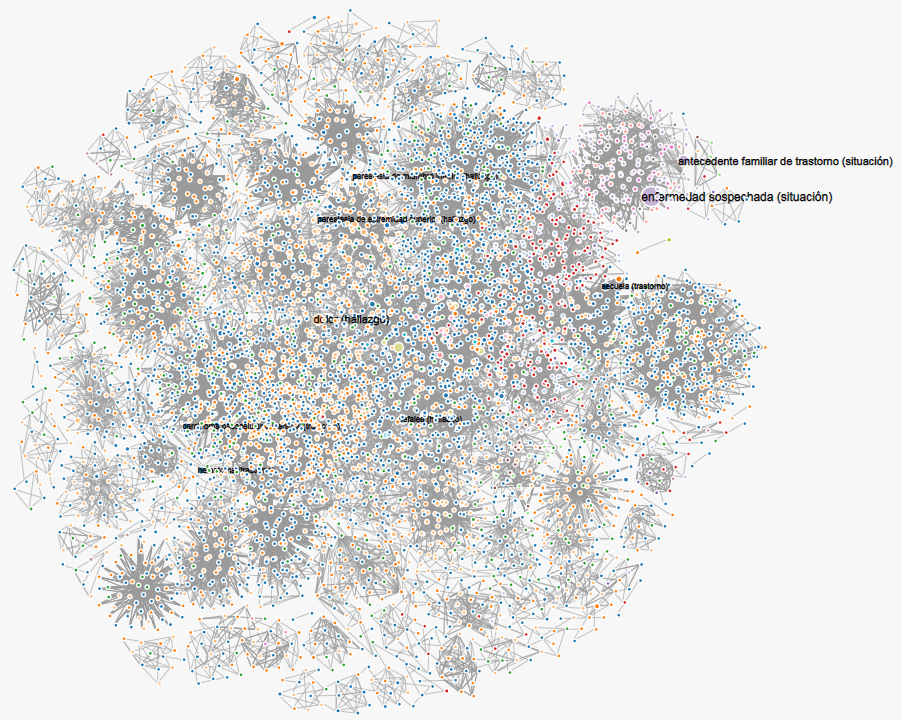
\includegraphics[width=\textwidth]{clust_todo}
\end{figure}

\begin{figure}[ht]
\caption{Agrupamientos del grafo de la lista de problemas en el contexto de los servicios de cardiología de adultos y pediátrica}
\label{fig:clust_area_cardio}
\centering
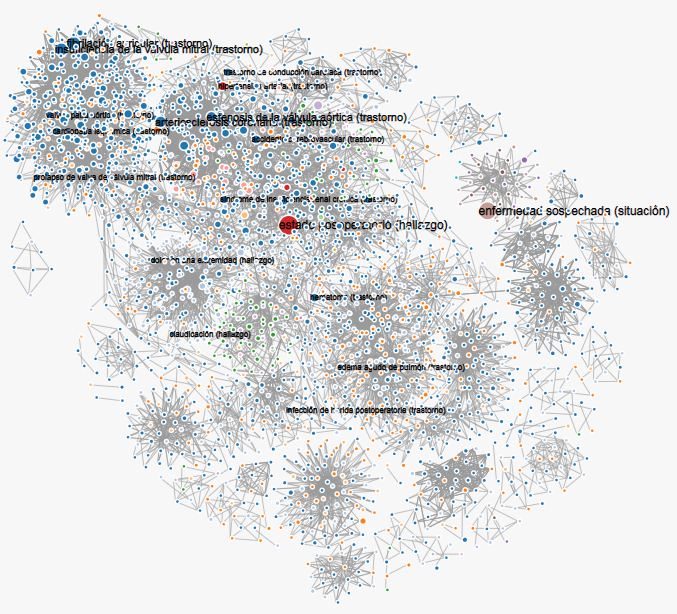
\includegraphics[width=\textwidth]{clust_area_cardio}
\end{figure}

\begin{figure}[ht]
\caption{Agrupamientos del grafo de la lista de problemas en el contexto del servicio de dermatología}
\label{fig:clust_area_dermatologia}
\centering
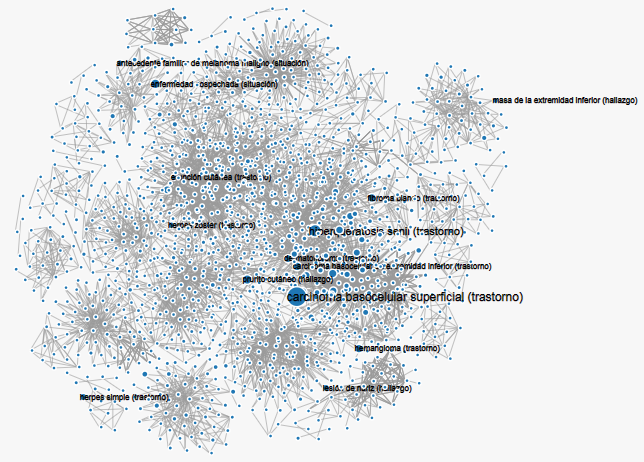
\includegraphics[width=\textwidth]{clust_area_dermatologia}
\end{figure}

\begin{figure}[ht]
\caption{Agrupamientos del grafo de la lista de problemas en el contexto de los servicios de endocrinología, nefrología y urología}
\label{fig:clust_area_ENU}
\centering
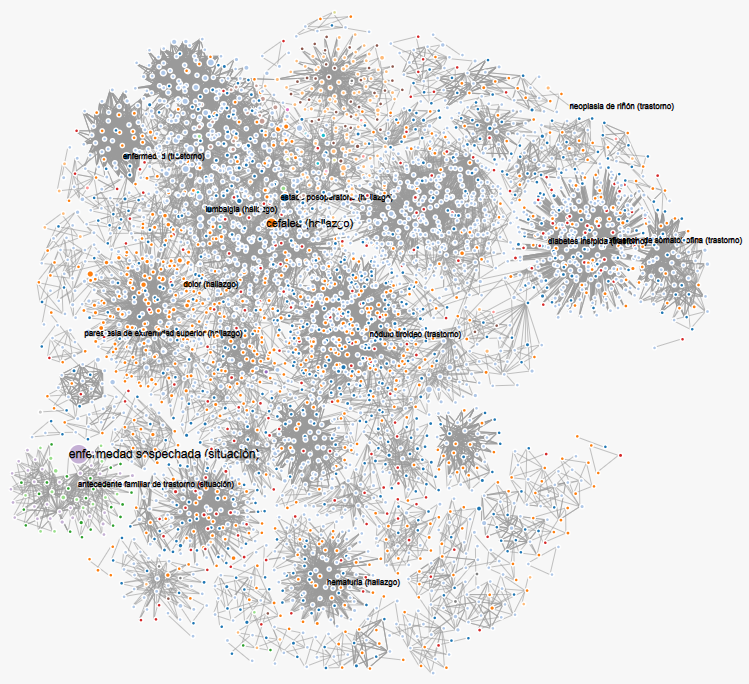
\includegraphics[width=\textwidth]{clust_area_ENU}
\end{figure}

\begin{figure}[ht]
\caption{Agrupamientos del grafo de la lista de problemas en el contexto del servicio de ginecobstreticia }
\label{fig:clust_area_gineco}
\centering
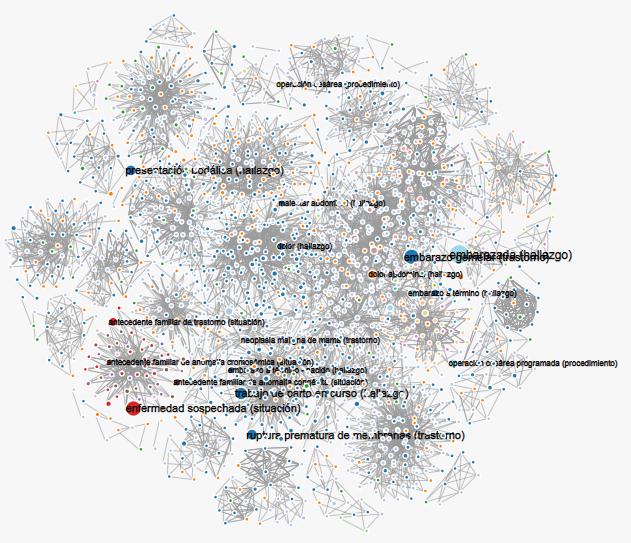
\includegraphics[width=\textwidth]{clust_area_gineco}
\end{figure}

\begin{figure}[ht]
\caption{Agrupamientos del grafo de la lista de problemas en el contexto del servicio de neurología }
\label{fig:clust_area_neuro}
\centering
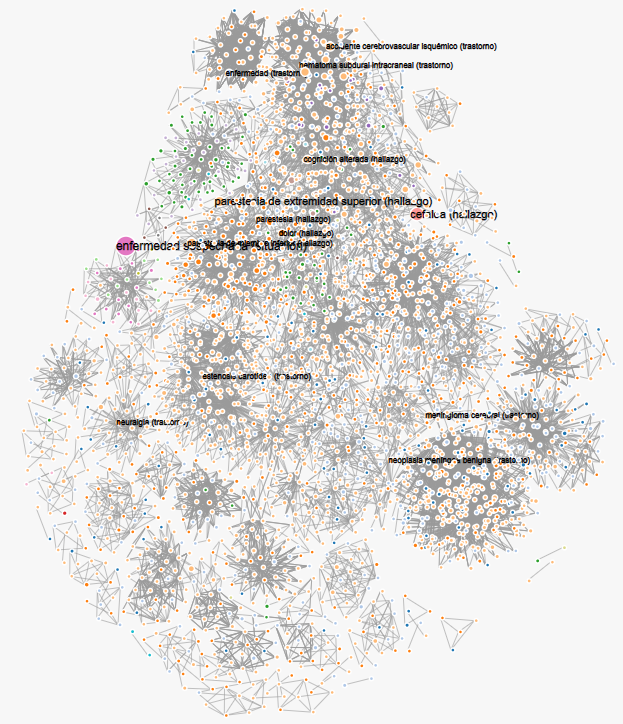
\includegraphics[width=\textwidth]{clust_area_neuro}
\end{figure}

\begin{figure}[ht]
\caption{Agrupamientos del grafo de la lista de problemas en el contexto del servicio de oftalmología }
\label{fig:clust_area_oftalmo}
\centering
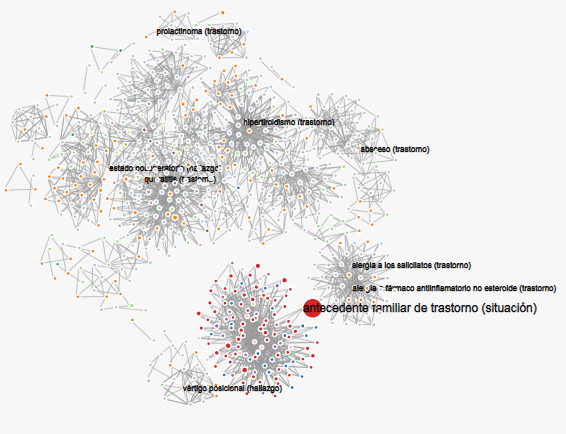
\includegraphics[width=\textwidth]{clust_area_oftalmo}
\end{figure}

\begin{figure}[ht]
\caption{Agrupamientos del grafo de la lista de problemas en el contexto del servicio de otorrinolaringología }
\label{fig:clust_area_otorrino}
\centering
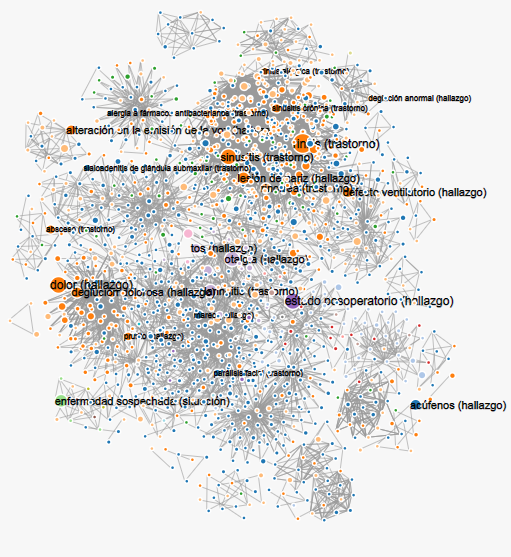
\includegraphics[width=\textwidth]{clust_area_otorrino}
\end{figure}

\begin{figure}[ht]
\caption{Agrupamientos del grafo de la lista de problemas en el contexto del servicio de pediatría }
\label{fig:clust_area_pedia}
\centering
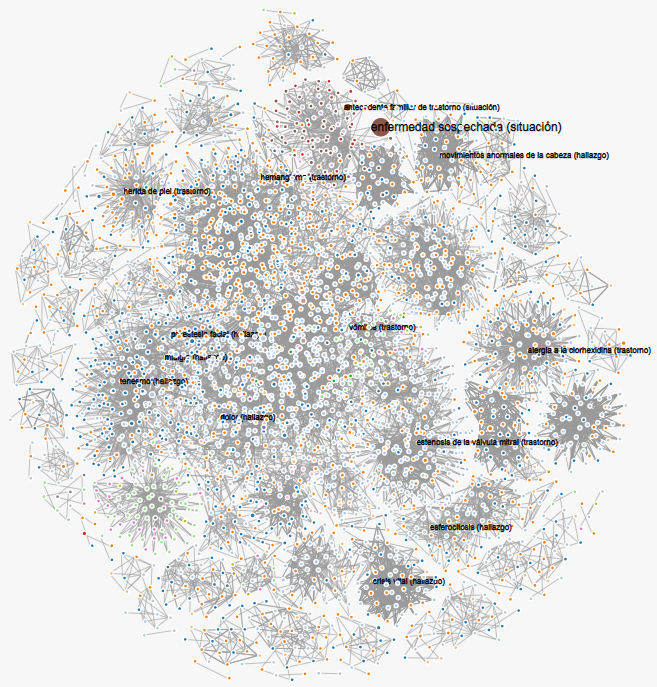
\includegraphics[width=\textwidth]{clust_area_pedia}
\end{figure}

\begin{figure}[ht]
\caption{Agrupamientos del grafo de la lista de problemas en el contexto del servicio de psiquiatría }
\label{fig:clust_area_psiqui}
\centering
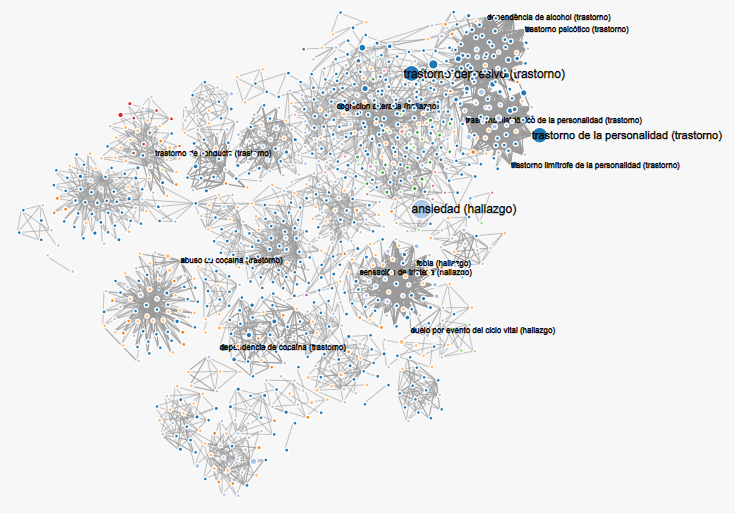
\includegraphics[width=\textwidth]{clust_area_psiqui}
\end{figure}

\begin{figure}[ht]
\caption{Agrupamientos del grafo de la lista de problemas en el contexto del servicio de traumatología }
\label{fig:clust_area_traumato}
\centering
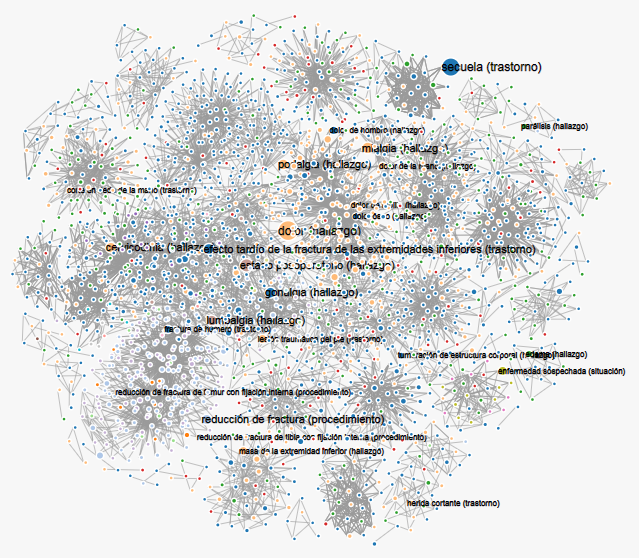
\includegraphics[width=\textwidth]{clust_area_traumato}
\end{figure}

\begin{figure}[ht]
\caption{Agrupamientos del grafo de la lista de problemas en el contexto del nivel asistencial ambulatorio }
\label{fig:clust_ambito_ambulatorio}
\centering
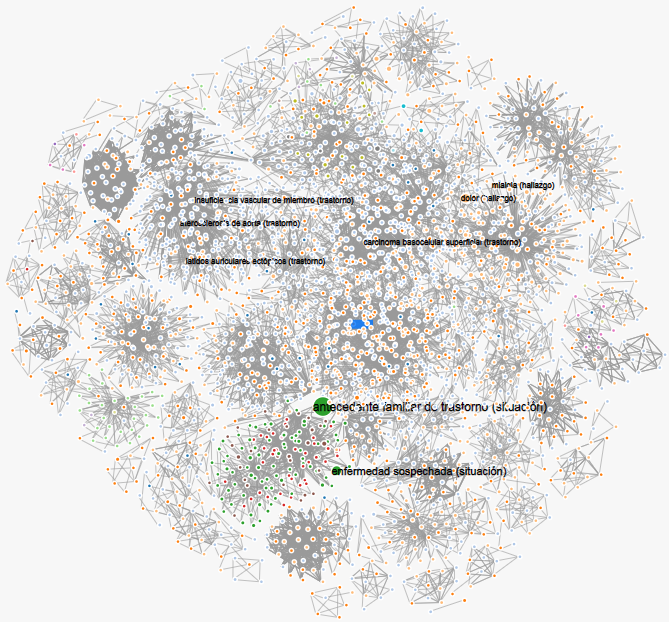
\includegraphics[width=\textwidth]{clust_ambito_1}
\end{figure}

\begin{figure}[ht]
\caption{Agrupamientos del grafo de la lista de problemas en el contexto del nivel asistencial de episodio ambulatorio }
\label{fig:clust_ambito_epi_ambulatorio}
\centering
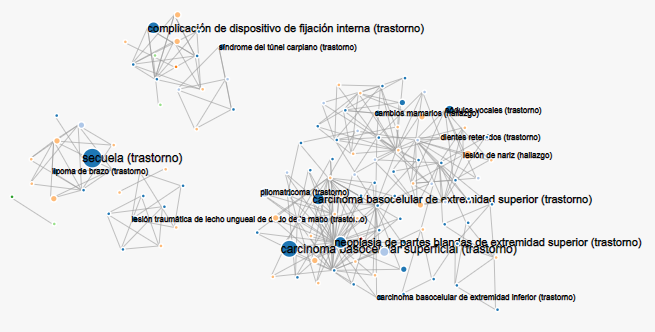
\includegraphics[width=\textwidth]{clust_ambito_9}
\end{figure}

\begin{figure}[ht]
\caption{Agrupamientos del grafo de la lista de problemas en el contexto del nivel asistencial de la guardia }
\label{fig:clust_ambito_guardia}
\centering
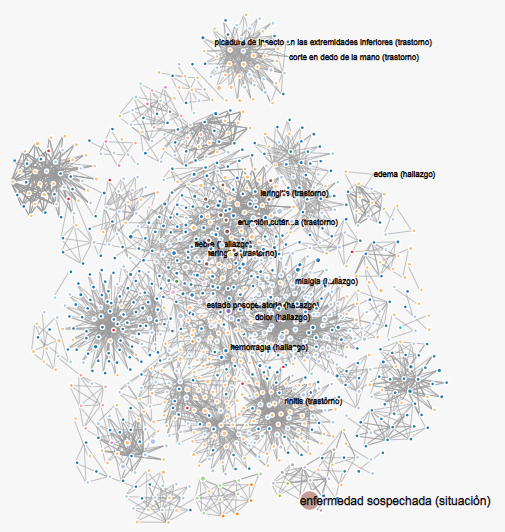
\includegraphics[width=\textwidth]{clust_ambito_3}
\end{figure}

\begin{figure}[ht]
\caption{Agrupamientos del grafo de la lista de problemas en el contexto del nivel asistencial de internación domiciliaria }
\label{fig:clust_ambito_inter_domici}
\centering
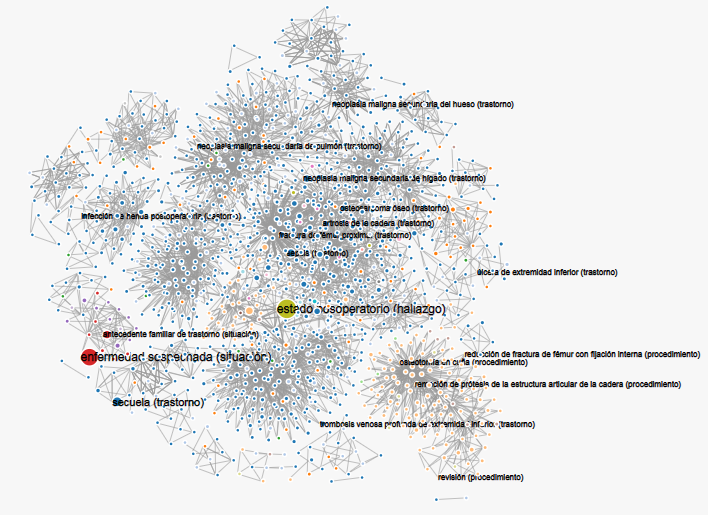
\includegraphics[width=\textwidth]{clust_ambito_6}
\end{figure}

\begin{figure}[ht]
\caption{Agrupamientos del grafo de la lista de problemas en el contexto del nivel asistencial de internación general }
\label{fig:clust_ambito_inter_general}
\centering
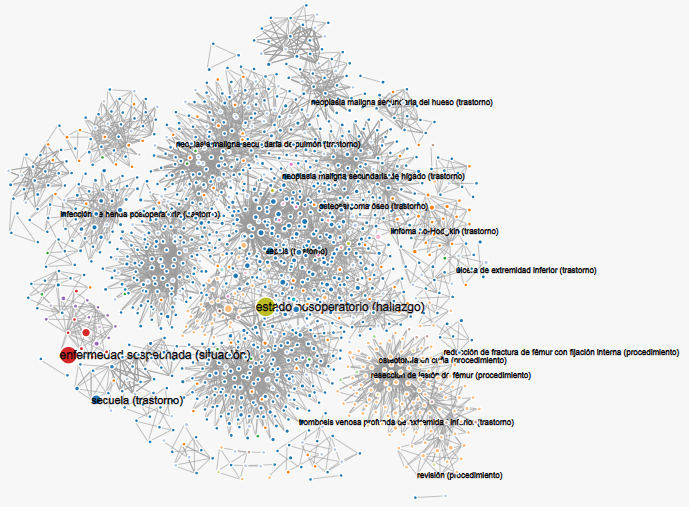
\includegraphics[width=\textwidth]{clust_ambito_2}
\end{figure}

\begin{figure}[ht]
\caption{Agrupamientos del grafo de la lista de problemas en el contexto del nivel asistencial del seguimiento domiciliario }
\label{fig:clust_ambito_segui_domici}
\centering
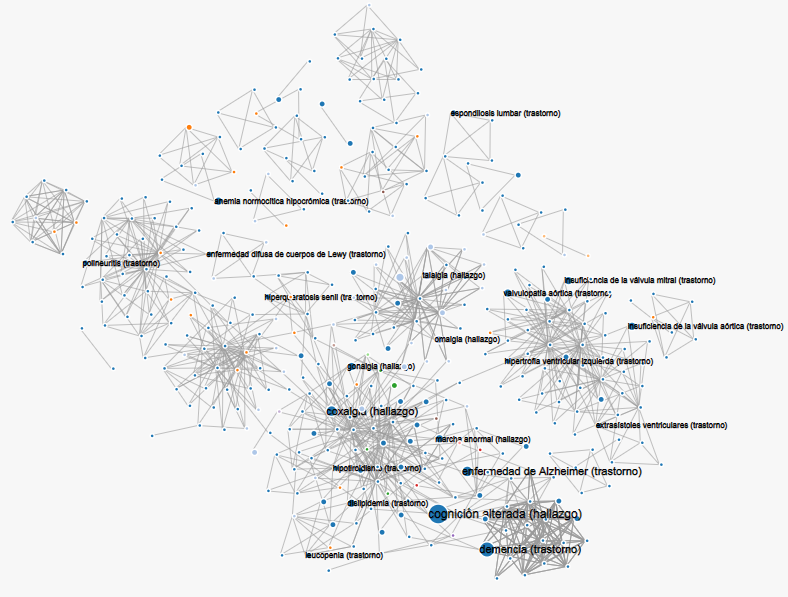
\includegraphics[width=\textwidth]{clust_ambito_7}
\end{figure}

\begin{figure}[ht]
\caption{Agrupamientos del grafo de la lista de problemas en el contexto del nivel asistencial del triage }
\label{fig:clust_ambito_triage}
\centering
\includegraphics[width=\textwidth]{clust_ambito_4}
\end{figure}

\begin{figure}[ht]
\caption{Agrupamientos del grafo de la lista de problemas en el contexto de grupo etario de 0 a 4, 15 a 24, 25 a 34 y 35 a 44 años }
\label{fig:clust_edad_0_4}
\centering
\includegraphics[width=\textwidth]{clust_edad_0-4}
\end{figure}

\begin{figure}[ht]
\caption{Agrupamientos del grafo de la lista de problemas en el contexto de grupo etario de 45 a 54 años }
\label{fig:clust_edad_45_54}
\centering
\includegraphics[width=\textwidth]{clust_edad_45-54}
\end{figure}

\begin{figure}[ht]
\caption{Agrupamientos del grafo de la lista de problemas en el contexto de grupo etario de 55 a 64 años }
\label{fig:clust_edad_55_64}
\centering
\includegraphics[width=\textwidth]{clust_edad_55-64}
\end{figure}

\begin{figure}[ht]
\caption{Agrupamientos del grafo de la lista de problemas en el contexto de grupo etario de 65 a 74 años }
\label{fig:clust_edad_65_74}
\centering
\includegraphics[width=\textwidth]{clust_edad_65-74}
\end{figure}

\begin{figure}[ht]
\caption{Agrupamientos del grafo de la lista de problemas en el contexto de grupo etario de 75 a 101 años }
\label{fig:clust_edad_75_101}
\centering
\includegraphics[width=\textwidth]{clust_edad_75-101}
\end{figure}

%%%% BIBLIOGRAFIA
\backmatter
\bibliographystyle{apacite}
\bibliography{Mendeley,otrosBiblio}



\end{document}
